\documentclass[twoside]{book}

% Packages required by doxygen
\usepackage{fixltx2e}
\usepackage{calc}
\usepackage{doxygen}
\usepackage[export]{adjustbox} % also loads graphicx
\usepackage{graphicx}
\usepackage[utf8]{inputenc}
\usepackage{makeidx}
\usepackage{multicol}
\usepackage{multirow}
\PassOptionsToPackage{warn}{textcomp}
\usepackage{textcomp}
\usepackage[nointegrals]{wasysym}
\usepackage[table]{xcolor}

% Font selection
\usepackage[T1]{fontenc}
\usepackage[scaled=.90]{helvet}
\usepackage{courier}
\usepackage{amssymb}
\usepackage{sectsty}
\renewcommand{\familydefault}{\sfdefault}
\allsectionsfont{%
  \fontseries{bc}\selectfont%
  \color{darkgray}%
}
\renewcommand{\DoxyLabelFont}{%
  \fontseries{bc}\selectfont%
  \color{darkgray}%
}
\newcommand{\+}{\discretionary{\mbox{\scriptsize$\hookleftarrow$}}{}{}}

% Page & text layout
\usepackage{geometry}
\geometry{%
  a4paper,%
  top=2.5cm,%
  bottom=2.5cm,%
  left=2.5cm,%
  right=2.5cm%
}
\tolerance=750
\hfuzz=15pt
\hbadness=750
\setlength{\emergencystretch}{15pt}
\setlength{\parindent}{0cm}
\setlength{\parskip}{3ex plus 2ex minus 2ex}
\makeatletter
\renewcommand{\paragraph}{%
  \@startsection{paragraph}{4}{0ex}{-1.0ex}{1.0ex}{%
    \normalfont\normalsize\bfseries\SS@parafont%
  }%
}
\renewcommand{\subparagraph}{%
  \@startsection{subparagraph}{5}{0ex}{-1.0ex}{1.0ex}{%
    \normalfont\normalsize\bfseries\SS@subparafont%
  }%
}
\makeatother

% Headers & footers
\usepackage{fancyhdr}
\pagestyle{fancyplain}
\fancyhead[LE]{\fancyplain{}{\bfseries\thepage}}
\fancyhead[CE]{\fancyplain{}{}}
\fancyhead[RE]{\fancyplain{}{\bfseries\leftmark}}
\fancyhead[LO]{\fancyplain{}{\bfseries\rightmark}}
\fancyhead[CO]{\fancyplain{}{}}
\fancyhead[RO]{\fancyplain{}{\bfseries\thepage}}
\fancyfoot[LE]{\fancyplain{}{}}
\fancyfoot[CE]{\fancyplain{}{}}
\fancyfoot[RE]{\fancyplain{}{\bfseries\scriptsize Generated by Doxygen }}
\fancyfoot[LO]{\fancyplain{}{\bfseries\scriptsize Generated by Doxygen }}
\fancyfoot[CO]{\fancyplain{}{}}
\fancyfoot[RO]{\fancyplain{}{}}
\renewcommand{\footrulewidth}{0.4pt}
\renewcommand{\chaptermark}[1]{%
  \markboth{#1}{}%
}
\renewcommand{\sectionmark}[1]{%
  \markright{\thesection\ #1}%
}

% Indices & bibliography
\usepackage{natbib}
\usepackage[titles]{tocloft}
\setcounter{tocdepth}{3}
\setcounter{secnumdepth}{5}
\makeindex

% Hyperlinks (required, but should be loaded last)
\usepackage{ifpdf}
\ifpdf
  \usepackage[pdftex,pagebackref=true]{hyperref}
\else
  \usepackage[ps2pdf,pagebackref=true]{hyperref}
\fi
\hypersetup{%
  colorlinks=true,%
  linkcolor=blue,%
  citecolor=blue,%
  unicode%
}

% Custom commands
\newcommand{\clearemptydoublepage}{%
  \newpage{\pagestyle{empty}\cleardoublepage}%
}

\usepackage{caption}
\captionsetup{labelsep=space,justification=centering,font={bf},singlelinecheck=off,skip=4pt,position=top}

%===== C O N T E N T S =====

\begin{document}

% Titlepage & ToC
\hypersetup{pageanchor=false,
             bookmarksnumbered=true,
             pdfencoding=unicode
            }
\pagenumbering{alph}
\begin{titlepage}
\vspace*{7cm}
\begin{center}%
{\Large Topaz }\\
\vspace*{1cm}
{\large Generated by Doxygen 1.8.14}\\
\end{center}
\end{titlepage}
\clearemptydoublepage
\pagenumbering{roman}
\tableofcontents
\clearemptydoublepage
\pagenumbering{arabic}
\hypersetup{pageanchor=true}

%--- Begin generated contents ---
\chapter{Namespace Index}
\section{Namespace List}
Here is a list of all documented namespaces with brief descriptions\+:\begin{DoxyCompactList}
\item\contentsline{section}{\mbox{\hyperlink{namespacetz}{tz}} }{\pageref{namespacetz}}{}
\item\contentsline{section}{\mbox{\hyperlink{namespacetz_1_1graphics_1_1model}{tz\+::graphics\+::model}} }{\pageref{namespacetz_1_1graphics_1_1model}}{}
\item\contentsline{section}{\mbox{\hyperlink{namespacetz_1_1graphics_1_1shader}{tz\+::graphics\+::shader}} }{\pageref{namespacetz_1_1graphics_1_1shader}}{}
\item\contentsline{section}{\mbox{\hyperlink{namespacetz_1_1transform}{tz\+::transform}} }{\pageref{namespacetz_1_1transform}}{}
\item\contentsline{section}{\mbox{\hyperlink{namespacetz_1_1util_1_1log}{tz\+::util\+::log}} }{\pageref{namespacetz_1_1util_1_1log}}{}
\item\contentsline{section}{\mbox{\hyperlink{namespacetz_1_1util_1_1string}{tz\+::util\+::string}} }{\pageref{namespacetz_1_1util_1_1string}}{}
\end{DoxyCompactList}

\chapter{Hierarchical Index}
\section{Class Hierarchy}
This inheritance list is sorted roughly, but not completely, alphabetically\+:\begin{DoxyCompactList}
\item \contentsline{section}{Audio\+Clip}{\pageref{class_audio_clip}}{}
\begin{DoxyCompactList}
\item \contentsline{section}{Audio\+Source}{\pageref{class_audio_source}}{}
\end{DoxyCompactList}
\item \contentsline{section}{Audio\+Music}{\pageref{class_audio_music}}{}
\item \contentsline{section}{Bitmap$<$ Pixel $>$}{\pageref{class_bitmap}}{}
\item \contentsline{section}{Boundary}{\pageref{class_boundary}}{}
\begin{DoxyCompactList}
\item \contentsline{section}{A\+A\+BB}{\pageref{class_a_a_b_b}}{}
\item \contentsline{section}{Bounding\+Plane}{\pageref{class_bounding_plane}}{}
\item \contentsline{section}{Bounding\+Sphere}{\pageref{class_bounding_sphere}}{}
\end{DoxyCompactList}
\item \contentsline{section}{Camera}{\pageref{class_camera}}{}
\item \contentsline{section}{Checkbox\+Choice}{\pageref{class_checkbox_choice}}{}
\item \contentsline{section}{Command}{\pageref{class_command}}{}
\begin{DoxyCompactList}
\item \contentsline{section}{Trivial\+Command}{\pageref{class_trivial_command}}{}
\begin{DoxyCompactList}
\item \contentsline{section}{Static\+Functor$<$ Functor, Functor\+Parameters $>$}{\pageref{class_static_functor}}{}
\item \contentsline{section}{Trivial\+Functor$<$ Functor $>$}{\pageref{class_trivial_functor}}{}
\end{DoxyCompactList}
\end{DoxyCompactList}
\item \contentsline{section}{Command\+Executor}{\pageref{class_command_executor}}{}
\item \contentsline{section}{Cube\+Map}{\pageref{class_cube_map}}{}
\item \contentsline{section}{Engine}{\pageref{class_engine}}{}
\item \contentsline{section}{Engine\+Meta}{\pageref{class_engine_meta}}{}
\item \contentsline{section}{Font}{\pageref{class_font}}{}
\item \contentsline{section}{Force}{\pageref{class_force}}{}
\item \contentsline{section}{Frame\+Buffer}{\pageref{class_frame_buffer}}{}
\item \contentsline{section}{Frustum}{\pageref{class_frustum}}{}
\item \contentsline{section}{Functor$<$ FunctorT $>$}{\pageref{class_functor}}{}
\item \contentsline{section}{G\+UI}{\pageref{class_g_u_i}}{}
\begin{DoxyCompactList}
\item \contentsline{section}{Panel}{\pageref{class_panel}}{}
\begin{DoxyCompactList}
\item \contentsline{section}{Checkbox}{\pageref{class_checkbox}}{}
\item \contentsline{section}{Slider}{\pageref{class_slider}}{}
\item \contentsline{section}{Text\+Label}{\pageref{class_text_label}}{}
\begin{DoxyCompactList}
\item \contentsline{section}{Button}{\pageref{class_button}}{}
\end{DoxyCompactList}
\end{DoxyCompactList}
\item \contentsline{section}{Window}{\pageref{class_window}}{}
\end{DoxyCompactList}
\item \contentsline{section}{tz\+:\+:graphics\+:\+:model\+:\+:Indexed\+Model}{\pageref{classtz_1_1graphics_1_1model_1_1_indexed_model}}{}
\item \contentsline{section}{Listener}{\pageref{class_listener}}{}
\begin{DoxyCompactList}
\item \contentsline{section}{Key\+Listener}{\pageref{class_key_listener}}{}
\item \contentsline{section}{Mouse\+Listener}{\pageref{class_mouse_listener}}{}
\end{DoxyCompactList}
\item \contentsline{section}{tz\+:\+:data\+:\+:Manager}{\pageref{classtz_1_1data_1_1_manager}}{}
\item \contentsline{section}{Material}{\pageref{class_material}}{}
\item \contentsline{section}{Matrix2x2}{\pageref{class_matrix2x2}}{}
\item \contentsline{section}{Matrix3x3}{\pageref{class_matrix3x3}}{}
\item \contentsline{section}{Matrix4x4}{\pageref{class_matrix4x4}}{}
\item M\+D\+L\+File\begin{DoxyCompactList}
\item \contentsline{section}{Properties\+File}{\pageref{class_properties_file}}{}
\item \contentsline{section}{Resources\+File}{\pageref{class_resources_file}}{}
\end{DoxyCompactList}
\item \contentsline{section}{Mesh}{\pageref{class_mesh}}{}
\begin{DoxyCompactList}
\item \contentsline{section}{Instanced\+Mesh}{\pageref{class_instanced_mesh}}{}
\end{DoxyCompactList}
\item \contentsline{section}{Object}{\pageref{class_object}}{}
\item \contentsline{section}{Object2D}{\pageref{class_object2_d}}{}
\begin{DoxyCompactList}
\item \contentsline{section}{Sprite}{\pageref{class_sprite}}{}
\end{DoxyCompactList}
\item \contentsline{section}{tz\+:\+:graphics\+:\+:model\+:\+:O\+B\+J\+Index}{\pageref{classtz_1_1graphics_1_1model_1_1_o_b_j_index}}{}
\item \contentsline{section}{tz\+:\+:graphics\+:\+:model\+:\+:O\+B\+J\+Model}{\pageref{classtz_1_1graphics_1_1model_1_1_o_b_j_model}}{}
\item \contentsline{section}{Pixel\+R\+G\+BA}{\pageref{class_pixel_r_g_b_a}}{}
\item \contentsline{section}{Random$<$ Engine, Engine\+Result\+Type $>$}{\pageref{class_random}}{}
\item \contentsline{section}{Render\+Buffer}{\pageref{class_render_buffer}}{}
\item \contentsline{section}{Scene}{\pageref{class_scene}}{}
\item \contentsline{section}{Shader}{\pageref{class_shader}}{}
\item \contentsline{section}{Skybox}{\pageref{class_skybox}}{}
\item \contentsline{section}{stbi\+\_\+io\+\_\+callbacks}{\pageref{structstbi__io__callbacks}}{}
\item \contentsline{section}{Texture}{\pageref{class_texture}}{}
\begin{DoxyCompactList}
\item \contentsline{section}{Displacement\+Map}{\pageref{class_displacement_map}}{}
\item \contentsline{section}{Normal\+Map}{\pageref{class_normal_map}}{}
\item \contentsline{section}{Parallax\+Map}{\pageref{class_parallax_map}}{}
\end{DoxyCompactList}
\item \contentsline{section}{Time\+Profiler}{\pageref{class_time_profiler}}{}
\item \contentsline{section}{Timer}{\pageref{class_timer}}{}
\item \contentsline{section}{Uniform\+Implicit}{\pageref{class_uniform_implicit}}{}
\begin{DoxyCompactList}
\item \contentsline{section}{Uniform$<$ T $>$}{\pageref{class_uniform}}{}
\end{DoxyCompactList}
\item \contentsline{section}{Vector$<$ N, T $>$}{\pageref{class_vector}}{}
\item \contentsline{section}{Vector2\+P\+OD}{\pageref{struct_vector2_p_o_d}}{}
\item \contentsline{section}{Vector3\+P\+OD}{\pageref{struct_vector3_p_o_d}}{}
\item \contentsline{section}{Vector4\+P\+OD}{\pageref{struct_vector4_p_o_d}}{}
\item \contentsline{section}{Vector$<$ 2, float $>$}{\pageref{class_vector}}{}
\begin{DoxyCompactList}
\item \contentsline{section}{Vector2$<$ float $>$}{\pageref{class_vector2}}{}
\end{DoxyCompactList}
\item \contentsline{section}{Vector$<$ 2, T $>$}{\pageref{class_vector}}{}
\begin{DoxyCompactList}
\item \contentsline{section}{Vector2$<$ T $>$}{\pageref{class_vector2}}{}
\end{DoxyCompactList}
\item \contentsline{section}{Vector$<$ 3, float $>$}{\pageref{class_vector}}{}
\begin{DoxyCompactList}
\item \contentsline{section}{Vector3$<$ float $>$}{\pageref{class_vector3}}{}
\end{DoxyCompactList}
\item \contentsline{section}{Vector$<$ 3, T $>$}{\pageref{class_vector}}{}
\begin{DoxyCompactList}
\item \contentsline{section}{Vector3$<$ T $>$}{\pageref{class_vector3}}{}
\end{DoxyCompactList}
\item \contentsline{section}{Vector$<$ 4, float $>$}{\pageref{class_vector}}{}
\begin{DoxyCompactList}
\item \contentsline{section}{Vector4$<$ float $>$}{\pageref{class_vector4}}{}
\begin{DoxyCompactList}
\item \contentsline{section}{Quaternion}{\pageref{class_quaternion}}{}
\end{DoxyCompactList}
\end{DoxyCompactList}
\item \contentsline{section}{Vector$<$ 4, T $>$}{\pageref{class_vector}}{}
\begin{DoxyCompactList}
\item \contentsline{section}{Vector4$<$ T $>$}{\pageref{class_vector4}}{}
\end{DoxyCompactList}
\item \contentsline{section}{Vector$<$ 4, unsigned char $>$}{\pageref{class_vector}}{}
\item \contentsline{section}{Vertex}{\pageref{class_vertex}}{}
\end{DoxyCompactList}

\chapter{Class Index}
\section{Class List}
Here are the classes, structs, unions and interfaces with brief descriptions\+:\begin{DoxyCompactList}
\item\contentsline{section}{\mbox{\hyperlink{class_a_a_b_b}{A\+A\+BB}} }{\pageref{class_a_a_b_b}}{}
\item\contentsline{section}{\mbox{\hyperlink{class_audio_clip}{Audio\+Clip}} }{\pageref{class_audio_clip}}{}
\item\contentsline{section}{\mbox{\hyperlink{class_audio_music}{Audio\+Music}} }{\pageref{class_audio_music}}{}
\item\contentsline{section}{\mbox{\hyperlink{class_audio_source}{Audio\+Source}} }{\pageref{class_audio_source}}{}
\item\contentsline{section}{\mbox{\hyperlink{class_bitmap}{Bitmap$<$ Pixel $>$}} }{\pageref{class_bitmap}}{}
\item\contentsline{section}{\mbox{\hyperlink{class_boundary}{Boundary}} }{\pageref{class_boundary}}{}
\item\contentsline{section}{\mbox{\hyperlink{class_bounding_plane}{Bounding\+Plane}} }{\pageref{class_bounding_plane}}{}
\item\contentsline{section}{\mbox{\hyperlink{class_bounding_sphere}{Bounding\+Sphere}} }{\pageref{class_bounding_sphere}}{}
\item\contentsline{section}{\mbox{\hyperlink{class_button}{Button}} }{\pageref{class_button}}{}
\item\contentsline{section}{\mbox{\hyperlink{class_camera}{Camera}} }{\pageref{class_camera}}{}
\item\contentsline{section}{\mbox{\hyperlink{class_checkbox}{Checkbox}} }{\pageref{class_checkbox}}{}
\item\contentsline{section}{\mbox{\hyperlink{class_checkbox_choice}{Checkbox\+Choice}} }{\pageref{class_checkbox_choice}}{}
\item\contentsline{section}{\mbox{\hyperlink{class_command}{Command}} }{\pageref{class_command}}{}
\item\contentsline{section}{\mbox{\hyperlink{class_command_executor}{Command\+Executor}} }{\pageref{class_command_executor}}{}
\item\contentsline{section}{\mbox{\hyperlink{class_cube_map}{Cube\+Map}} }{\pageref{class_cube_map}}{}
\item\contentsline{section}{\mbox{\hyperlink{class_displacement_map}{Displacement\+Map}} }{\pageref{class_displacement_map}}{}
\item\contentsline{section}{\mbox{\hyperlink{class_engine}{Engine}} }{\pageref{class_engine}}{}
\item\contentsline{section}{\mbox{\hyperlink{class_entity}{Entity}} }{\pageref{class_entity}}{}
\item\contentsline{section}{\mbox{\hyperlink{class_entity_object}{Entity\+Object}} }{\pageref{class_entity_object}}{}
\item\contentsline{section}{\mbox{\hyperlink{class_font}{Font}} }{\pageref{class_font}}{}
\item\contentsline{section}{\mbox{\hyperlink{class_force}{Force}} }{\pageref{class_force}}{}
\item\contentsline{section}{\mbox{\hyperlink{class_frame_buffer}{Frame\+Buffer}} }{\pageref{class_frame_buffer}}{}
\item\contentsline{section}{\mbox{\hyperlink{class_functor}{Functor$<$ Functor\+T $>$}} }{\pageref{class_functor}}{}
\item\contentsline{section}{\mbox{\hyperlink{class_g_u_i}{G\+UI}} }{\pageref{class_g_u_i}}{}
\item\contentsline{section}{\mbox{\hyperlink{classtz_1_1graphics_1_1model_1_1_indexed_model}{tz\+::graphics\+::model\+::\+Indexed\+Model}} }{\pageref{classtz_1_1graphics_1_1model_1_1_indexed_model}}{}
\item\contentsline{section}{\mbox{\hyperlink{class_instanced_mesh}{Instanced\+Mesh}} }{\pageref{class_instanced_mesh}}{}
\item\contentsline{section}{\mbox{\hyperlink{class_key_listener}{Key\+Listener}} }{\pageref{class_key_listener}}{}
\item\contentsline{section}{\mbox{\hyperlink{class_listener}{Listener}} }{\pageref{class_listener}}{}
\item\contentsline{section}{\mbox{\hyperlink{classtz_1_1data_1_1_manager}{tz\+::data\+::\+Manager}} }{\pageref{classtz_1_1data_1_1_manager}}{}
\item\contentsline{section}{\mbox{\hyperlink{class_material}{Material}} }{\pageref{class_material}}{}
\item\contentsline{section}{\mbox{\hyperlink{class_matrix2x2}{Matrix2x2}} }{\pageref{class_matrix2x2}}{}
\item\contentsline{section}{\mbox{\hyperlink{class_matrix3x3}{Matrix3x3}} }{\pageref{class_matrix3x3}}{}
\item\contentsline{section}{\mbox{\hyperlink{class_matrix4x4}{Matrix4x4}} }{\pageref{class_matrix4x4}}{}
\item\contentsline{section}{\mbox{\hyperlink{class_mesh}{Mesh}} }{\pageref{class_mesh}}{}
\item\contentsline{section}{\mbox{\hyperlink{class_mouse_listener}{Mouse\+Listener}} }{\pageref{class_mouse_listener}}{}
\item\contentsline{section}{\mbox{\hyperlink{class_normal_map}{Normal\+Map}} }{\pageref{class_normal_map}}{}
\item\contentsline{section}{\mbox{\hyperlink{class_object}{Object}} }{\pageref{class_object}}{}
\item\contentsline{section}{\mbox{\hyperlink{class_object2_d}{Object2D}} }{\pageref{class_object2_d}}{}
\item\contentsline{section}{\mbox{\hyperlink{classtz_1_1graphics_1_1model_1_1_o_b_j_index}{tz\+::graphics\+::model\+::\+O\+B\+J\+Index}} }{\pageref{classtz_1_1graphics_1_1model_1_1_o_b_j_index}}{}
\item\contentsline{section}{\mbox{\hyperlink{classtz_1_1graphics_1_1model_1_1_o_b_j_model}{tz\+::graphics\+::model\+::\+O\+B\+J\+Model}} }{\pageref{classtz_1_1graphics_1_1model_1_1_o_b_j_model}}{}
\item\contentsline{section}{\mbox{\hyperlink{class_panel}{Panel}} }{\pageref{class_panel}}{}
\item\contentsline{section}{\mbox{\hyperlink{class_parallax_map}{Parallax\+Map}} }{\pageref{class_parallax_map}}{}
\item\contentsline{section}{\mbox{\hyperlink{class_pixel_r_g_b_a}{Pixel\+R\+G\+BA}} }{\pageref{class_pixel_r_g_b_a}}{}
\item\contentsline{section}{\mbox{\hyperlink{class_quaternion}{Quaternion}} }{\pageref{class_quaternion}}{}
\item\contentsline{section}{\mbox{\hyperlink{class_random}{Random$<$ Engine, Engine\+Result\+Type $>$}} }{\pageref{class_random}}{}
\item\contentsline{section}{\mbox{\hyperlink{class_render_buffer}{Render\+Buffer}} }{\pageref{class_render_buffer}}{}
\item\contentsline{section}{\mbox{\hyperlink{class_scene}{Scene}} }{\pageref{class_scene}}{}
\item\contentsline{section}{\mbox{\hyperlink{class_shader}{Shader}} }{\pageref{class_shader}}{}
\item\contentsline{section}{\mbox{\hyperlink{class_skybox}{Skybox}} }{\pageref{class_skybox}}{}
\item\contentsline{section}{\mbox{\hyperlink{class_slider}{Slider}} }{\pageref{class_slider}}{}
\item\contentsline{section}{\mbox{\hyperlink{class_sprite}{Sprite}} }{\pageref{class_sprite}}{}
\item\contentsline{section}{\mbox{\hyperlink{class_static_functor}{Static\+Functor$<$ Functor, Functor\+Parameters $>$}} }{\pageref{class_static_functor}}{}
\item\contentsline{section}{\mbox{\hyperlink{structstbi__io__callbacks}{stbi\+\_\+io\+\_\+callbacks}} }{\pageref{structstbi__io__callbacks}}{}
\item\contentsline{section}{\mbox{\hyperlink{class_text_label}{Text\+Label}} }{\pageref{class_text_label}}{}
\item\contentsline{section}{\mbox{\hyperlink{class_texture}{Texture}} }{\pageref{class_texture}}{}
\item\contentsline{section}{\mbox{\hyperlink{class_time_profiler}{Time\+Profiler}} }{\pageref{class_time_profiler}}{}
\item\contentsline{section}{\mbox{\hyperlink{class_timer}{Timer}} }{\pageref{class_timer}}{}
\item\contentsline{section}{\mbox{\hyperlink{class_trivial_command}{Trivial\+Command}} }{\pageref{class_trivial_command}}{}
\item\contentsline{section}{\mbox{\hyperlink{class_trivial_functor}{Trivial\+Functor$<$ Functor $>$}} }{\pageref{class_trivial_functor}}{}
\item\contentsline{section}{\mbox{\hyperlink{class_uniform}{Uniform$<$ T $>$}} }{\pageref{class_uniform}}{}
\item\contentsline{section}{\mbox{\hyperlink{class_uniform_implicit}{Uniform\+Implicit}} }{\pageref{class_uniform_implicit}}{}
\item\contentsline{section}{\mbox{\hyperlink{class_vector2}{Vector2$<$ T $>$}} }{\pageref{class_vector2}}{}
\item\contentsline{section}{\mbox{\hyperlink{struct_vector2_p_o_d}{Vector2\+P\+OD}} }{\pageref{struct_vector2_p_o_d}}{}
\item\contentsline{section}{\mbox{\hyperlink{class_vector3}{Vector3$<$ T $>$}} }{\pageref{class_vector3}}{}
\item\contentsline{section}{\mbox{\hyperlink{struct_vector3_p_o_d}{Vector3\+P\+OD}} }{\pageref{struct_vector3_p_o_d}}{}
\item\contentsline{section}{\mbox{\hyperlink{class_vector4}{Vector4$<$ T $>$}} }{\pageref{class_vector4}}{}
\item\contentsline{section}{\mbox{\hyperlink{struct_vector4_p_o_d}{Vector4\+P\+OD}} }{\pageref{struct_vector4_p_o_d}}{}
\item\contentsline{section}{\mbox{\hyperlink{class_vertex}{Vertex}} }{\pageref{class_vertex}}{}
\item\contentsline{section}{\mbox{\hyperlink{class_window}{Window}} }{\pageref{class_window}}{}
\end{DoxyCompactList}

\chapter{Namespace Documentation}
\hypertarget{namespacetz}{}\section{tz Namespace Reference}
\label{namespacetz}\index{tz@{tz}}
\subsection*{Namespaces}
\begin{DoxyCompactItemize}
\item 
 \mbox{\hyperlink{namespacetz_1_1transform}{transform}}
\end{DoxyCompactItemize}
\subsection*{Functions}
\begin{DoxyCompactItemize}
\item 
void \mbox{\hyperlink{namespacetz_aeb2530fee0e452e5ba5f4d0d0ebaa797}{initialise}} ()
\item 
void \mbox{\hyperlink{namespacetz_a0a5d1e375e7e82fcd12a8b74b8012bae}{terminate}} ()
\end{DoxyCompactItemize}
\subsection*{Variables}
\begin{DoxyCompactItemize}
\item 
\mbox{\Hypertarget{namespacetz_ad65b104d9b1d4740bf069e7d33a2da1d}\label{namespacetz_ad65b104d9b1d4740bf069e7d33a2da1d}} 
constexpr char {\bfseries default\+\_\+properties\+\_\+path} \mbox{[}$\,$\mbox{]} = \char`\"{}properties.\+mdl\char`\"{}
\end{DoxyCompactItemize}


\subsection{Detailed Description}
Initialise and terminate tz audio module. This must be done appropriately to use any of the audio functionality. 

\subsection{Function Documentation}
\mbox{\Hypertarget{namespacetz_aeb2530fee0e452e5ba5f4d0d0ebaa797}\label{namespacetz_aeb2530fee0e452e5ba5f4d0d0ebaa797}} 
\index{tz@{tz}!initialise@{initialise}}
\index{initialise@{initialise}!tz@{tz}}
\subsubsection{\texorpdfstring{initialise()}{initialise()}}
{\footnotesize\ttfamily void tz\+::initialise (\begin{DoxyParamCaption}{ }\end{DoxyParamCaption})\hspace{0.3cm}{\ttfamily [inline]}}

Invoke this to initialise all Topaz modules and be able to use all features. Note that a Topaz window must have been constructed at least once before the graphics module fully initialises.

No audio works until this is executed. \mbox{\hyperlink{namespacetz_aeb2530fee0e452e5ba5f4d0d0ebaa797}{tz\+::initialise}} will invoke this automatically.

Initialises the graphics component of Topaz. An Open\+GL window-\/context M\+U\+ST exist before this is executed. Topaz \mbox{\hyperlink{class_window}{Window}} constructor invokes this upon first invocation. If you are not using Topaz windows, you will have to invoke this yourself. If you are using Topaz windows, DO N\+OT T\+O\+U\+CH T\+H\+IS. \mbox{\Hypertarget{namespacetz_a0a5d1e375e7e82fcd12a8b74b8012bae}\label{namespacetz_a0a5d1e375e7e82fcd12a8b74b8012bae}} 
\index{tz@{tz}!terminate@{terminate}}
\index{terminate@{terminate}!tz@{tz}}
\subsubsection{\texorpdfstring{terminate()}{terminate()}}
{\footnotesize\ttfamily void tz\+::terminate (\begin{DoxyParamCaption}{ }\end{DoxyParamCaption})\hspace{0.3cm}{\ttfamily [inline]}}

Invoke this to close all Topaz modules and free corresponding memory to prevent droplets Once this function is executed, most features will cease to work properly and will likely invoke undefined behaviour.

Memory droplets will remain until this is executed. Audio will not work after this is invoked. \mbox{\hyperlink{namespacetz_a0a5d1e375e7e82fcd12a8b74b8012bae}{tz\+::terminate}} will invoke this automatically.

Terminates and destroys all graphics components of Topaz. \mbox{\hyperlink{namespacetz_a0a5d1e375e7e82fcd12a8b74b8012bae}{tz\+::terminate}} will invoke this automatically. Only use this function if you do not wish to use \mbox{\hyperlink{namespacetz_a0a5d1e375e7e82fcd12a8b74b8012bae}{tz\+::terminate}} to terminate all features, but instead cherry-\/pick components like graphics. 
\hypertarget{namespacetz_1_1graphics_1_1model}{}\section{tz\+:\+:graphics\+:\+:model Namespace Reference}
\label{namespacetz_1_1graphics_1_1model}\index{tz\+::graphics\+::model@{tz\+::graphics\+::model}}
\subsection*{Classes}
\begin{DoxyCompactItemize}
\item 
class \mbox{\hyperlink{classtz_1_1graphics_1_1model_1_1_indexed_model}{Indexed\+Model}}
\item 
class \mbox{\hyperlink{classtz_1_1graphics_1_1model_1_1_o_b_j_index}{O\+B\+J\+Index}}
\item 
class \mbox{\hyperlink{classtz_1_1graphics_1_1model_1_1_o_b_j_model}{O\+B\+J\+Model}}
\end{DoxyCompactItemize}


\subsection{Detailed Description}
Currently used only for Wavefront O\+BJ Models. To load an O\+BJ model in Topaz, invoke O\+B\+J\+Model\+::to\+Indexed\+Model to receive an instance of \mbox{\hyperlink{classtz_1_1graphics_1_1model_1_1_indexed_model}{Indexed\+Model}}. A Topaz \mbox{\hyperlink{class_mesh}{Mesh}} constructor can take an \mbox{\hyperlink{classtz_1_1graphics_1_1model_1_1_indexed_model}{Indexed\+Model}} as a parameter. 
\hypertarget{namespacetz_1_1graphics_1_1shader}{}\section{tz\+:\+:graphics\+:\+:shader Namespace Reference}
\label{namespacetz_1_1graphics_1_1shader}\index{tz\+::graphics\+::shader@{tz\+::graphics\+::shader}}
\subsection*{Functions}
\begin{DoxyCompactItemize}
\item 
\mbox{\Hypertarget{namespacetz_1_1graphics_1_1shader_a43ad94b340d47ed1ce9c10c026a7cac5}\label{namespacetz_1_1graphics_1_1shader_a43ad94b340d47ed1ce9c10c026a7cac5}} 
\mbox{\hyperlink{class_shader}{Shader}} {\bfseries pass\+\_\+through} (std\+::string position\+\_\+attribute\+\_\+name=\char`\"{}position\+\_\+modelspace\+\_\+attribute\char`\"{}, std\+::string texture\+\_\+coordinate\+\_\+attribute\+\_\+name=\char`\"{}texture\+\_\+coordinate\+\_\+attribute\char`\"{}, std\+::string texture\+\_\+sampler\+\_\+name=\char`\"{}texture\+\_\+sampler\+\_\+uniform\char`\"{})
\end{DoxyCompactItemize}


\subsection{Detailed Description}
Factory functions for Shaders that need no special source code; simply pass-\/through shaders and the ability to render 3D geometry, with some plain old textures. If your application is so simple that only the simplest matrix transformations are needed with no fancy effects, use this. 
\hypertarget{namespacetz_1_1transform}{}\section{tz\+:\+:transform Namespace Reference}
\label{namespacetz_1_1transform}\index{tz\+::transform@{tz\+::transform}}
\subsection*{Functions}
\begin{DoxyCompactItemize}
\item 
\mbox{\hyperlink{class_matrix4x4}{Matrix4x4}} \mbox{\hyperlink{namespacetz_1_1transform_aaf7c616e2645fda6e6e38899bfd52119}{translate}} (const \mbox{\hyperlink{class_vector3}{Vector3F}} \&position)
\item 
\mbox{\hyperlink{class_matrix4x4}{Matrix4x4}} \mbox{\hyperlink{namespacetz_1_1transform_a41841500a4f61978a446b7a92a982c61}{rotate\+\_\+x}} (float euler\+\_\+x)
\item 
\mbox{\hyperlink{class_matrix4x4}{Matrix4x4}} \mbox{\hyperlink{namespacetz_1_1transform_ad4f8e1471ddc14c62c3247f4335780a5}{rotate\+\_\+y}} (float euler\+\_\+y)
\item 
\mbox{\hyperlink{class_matrix4x4}{Matrix4x4}} \mbox{\hyperlink{namespacetz_1_1transform_a1fc9b0958f30aba9c97d55bc25fde583}{rotate\+\_\+z}} (float euler\+\_\+z)
\item 
\mbox{\hyperlink{class_matrix4x4}{Matrix4x4}} \mbox{\hyperlink{namespacetz_1_1transform_aeeb88eb1d2cd9565afb0cca2ab011f89}{rotate}} (const \mbox{\hyperlink{class_vector3}{Vector3F}} \&euler\+\_\+rotation)
\item 
\mbox{\hyperlink{class_matrix4x4}{Matrix4x4}} \mbox{\hyperlink{namespacetz_1_1transform_a662bede6ecd13fd3555d612a06c350cf}{scale}} (const \mbox{\hyperlink{class_vector3}{Vector3F}} \&scale)
\item 
\mbox{\hyperlink{class_matrix4x4}{Matrix4x4}} \mbox{\hyperlink{namespacetz_1_1transform_a0cf7e4695205f96b42fcb9fd316193d7}{model}} (const \mbox{\hyperlink{class_vector3}{Vector3F}} \&position, const \mbox{\hyperlink{class_vector3}{Vector3F}} \&euler\+\_\+rotation, const \mbox{\hyperlink{class_vector3}{Vector3F}} \&\mbox{\hyperlink{namespacetz_1_1transform_a662bede6ecd13fd3555d612a06c350cf}{scale}})
\item 
\mbox{\hyperlink{class_matrix4x4}{Matrix4x4}} \mbox{\hyperlink{namespacetz_1_1transform_af50903633804f4488c75cfc54d5100dc}{view}} (const \mbox{\hyperlink{class_vector3}{Vector3F}} \&camera\+\_\+position, const \mbox{\hyperlink{class_vector3}{Vector3F}} \&camera\+\_\+euler\+\_\+rotation)
\item 
\mbox{\hyperlink{class_matrix4x4}{Matrix4x4}} \mbox{\hyperlink{namespacetz_1_1transform_a8a5b3be2af4fcc2bb4c92a42bdd563ae}{orthographic\+\_\+projection}} (float right, float left, float top, float bottom, float near, float far)
\item 
\mbox{\hyperlink{class_matrix4x4}{Matrix4x4}} \mbox{\hyperlink{namespacetz_1_1transform_aadc949f1b24a655a504e9a7ead18e2b2}{perspective\+\_\+projection}} (float fov, float width, float height, float nearclip, float farclip)
\end{DoxyCompactItemize}


\subsection{Detailed Description}
Topaz transformation matrices are always in row-\/major format. 

\subsection{Function Documentation}
\mbox{\Hypertarget{namespacetz_1_1transform_a0cf7e4695205f96b42fcb9fd316193d7}\label{namespacetz_1_1transform_a0cf7e4695205f96b42fcb9fd316193d7}} 
\index{tz\+::transform@{tz\+::transform}!model@{model}}
\index{model@{model}!tz\+::transform@{tz\+::transform}}
\subsubsection{\texorpdfstring{model()}{model()}}
{\footnotesize\ttfamily \mbox{\hyperlink{class_matrix4x4}{Matrix4x4}} tz\+::transform\+::model (\begin{DoxyParamCaption}\item[{const \mbox{\hyperlink{class_vector3}{Vector3F}} \&}]{position,  }\item[{const \mbox{\hyperlink{class_vector3}{Vector3F}} \&}]{euler\+\_\+rotation,  }\item[{const \mbox{\hyperlink{class_vector3}{Vector3F}} \&}]{scale }\end{DoxyParamCaption})}

Construct a row-\/major model matrix using the functions above. \mbox{\Hypertarget{namespacetz_1_1transform_a8a5b3be2af4fcc2bb4c92a42bdd563ae}\label{namespacetz_1_1transform_a8a5b3be2af4fcc2bb4c92a42bdd563ae}} 
\index{tz\+::transform@{tz\+::transform}!orthographic\+\_\+projection@{orthographic\+\_\+projection}}
\index{orthographic\+\_\+projection@{orthographic\+\_\+projection}!tz\+::transform@{tz\+::transform}}
\subsubsection{\texorpdfstring{orthographic\+\_\+projection()}{orthographic\_projection()}}
{\footnotesize\ttfamily \mbox{\hyperlink{class_matrix4x4}{Matrix4x4}} tz\+::transform\+::orthographic\+\_\+projection (\begin{DoxyParamCaption}\item[{float}]{right,  }\item[{float}]{left,  }\item[{float}]{top,  }\item[{float}]{bottom,  }\item[{float}]{near,  }\item[{float}]{far }\end{DoxyParamCaption})}

Construct a row-\/major projection matrix to create an orthographic projection. \mbox{\Hypertarget{namespacetz_1_1transform_aadc949f1b24a655a504e9a7ead18e2b2}\label{namespacetz_1_1transform_aadc949f1b24a655a504e9a7ead18e2b2}} 
\index{tz\+::transform@{tz\+::transform}!perspective\+\_\+projection@{perspective\+\_\+projection}}
\index{perspective\+\_\+projection@{perspective\+\_\+projection}!tz\+::transform@{tz\+::transform}}
\subsubsection{\texorpdfstring{perspective\+\_\+projection()}{perspective\_projection()}}
{\footnotesize\ttfamily \mbox{\hyperlink{class_matrix4x4}{Matrix4x4}} tz\+::transform\+::perspective\+\_\+projection (\begin{DoxyParamCaption}\item[{float}]{fov,  }\item[{float}]{width,  }\item[{float}]{height,  }\item[{float}]{near\+\_\+clip,  }\item[{float}]{far\+\_\+clip }\end{DoxyParamCaption})}

Construct a row-\/major projection matrix to create a perspective projection. Use this to simulate 3D with a \char`\"{}camera\char`\"{}. \mbox{\Hypertarget{namespacetz_1_1transform_aeeb88eb1d2cd9565afb0cca2ab011f89}\label{namespacetz_1_1transform_aeeb88eb1d2cd9565afb0cca2ab011f89}} 
\index{tz\+::transform@{tz\+::transform}!rotate@{rotate}}
\index{rotate@{rotate}!tz\+::transform@{tz\+::transform}}
\subsubsection{\texorpdfstring{rotate()}{rotate()}}
{\footnotesize\ttfamily \mbox{\hyperlink{class_matrix4x4}{Matrix4x4}} tz\+::transform\+::rotate (\begin{DoxyParamCaption}\item[{const \mbox{\hyperlink{class_vector3}{Vector3F}} \&}]{euler\+\_\+rotation }\end{DoxyParamCaption})}

Construct a four-\/dimensional row-\/major rotational matrix using X\+YZ rotations (Pitch, Yaw, Roll in Euler-\/angles). \mbox{\Hypertarget{namespacetz_1_1transform_a41841500a4f61978a446b7a92a982c61}\label{namespacetz_1_1transform_a41841500a4f61978a446b7a92a982c61}} 
\index{tz\+::transform@{tz\+::transform}!rotate\+\_\+x@{rotate\+\_\+x}}
\index{rotate\+\_\+x@{rotate\+\_\+x}!tz\+::transform@{tz\+::transform}}
\subsubsection{\texorpdfstring{rotate\+\_\+x()}{rotate\_x()}}
{\footnotesize\ttfamily \mbox{\hyperlink{class_matrix4x4}{Matrix4x4}} tz\+::transform\+::rotate\+\_\+x (\begin{DoxyParamCaption}\item[{float}]{euler\+\_\+x }\end{DoxyParamCaption})}

Construct a four-\/dimensional row-\/major rotational matrix in the x-\/axis (Pitch). \mbox{\Hypertarget{namespacetz_1_1transform_ad4f8e1471ddc14c62c3247f4335780a5}\label{namespacetz_1_1transform_ad4f8e1471ddc14c62c3247f4335780a5}} 
\index{tz\+::transform@{tz\+::transform}!rotate\+\_\+y@{rotate\+\_\+y}}
\index{rotate\+\_\+y@{rotate\+\_\+y}!tz\+::transform@{tz\+::transform}}
\subsubsection{\texorpdfstring{rotate\+\_\+y()}{rotate\_y()}}
{\footnotesize\ttfamily \mbox{\hyperlink{class_matrix4x4}{Matrix4x4}} tz\+::transform\+::rotate\+\_\+y (\begin{DoxyParamCaption}\item[{float}]{euler\+\_\+y }\end{DoxyParamCaption})}

Construct a four-\/dimensional row-\/major rotational matrix in the y-\/axis (Yaw). \mbox{\Hypertarget{namespacetz_1_1transform_a1fc9b0958f30aba9c97d55bc25fde583}\label{namespacetz_1_1transform_a1fc9b0958f30aba9c97d55bc25fde583}} 
\index{tz\+::transform@{tz\+::transform}!rotate\+\_\+z@{rotate\+\_\+z}}
\index{rotate\+\_\+z@{rotate\+\_\+z}!tz\+::transform@{tz\+::transform}}
\subsubsection{\texorpdfstring{rotate\+\_\+z()}{rotate\_z()}}
{\footnotesize\ttfamily \mbox{\hyperlink{class_matrix4x4}{Matrix4x4}} tz\+::transform\+::rotate\+\_\+z (\begin{DoxyParamCaption}\item[{float}]{euler\+\_\+z }\end{DoxyParamCaption})}

Construct a four-\/dimensional row-\/major rotational matrix in the x-\/axis (Roll). \mbox{\Hypertarget{namespacetz_1_1transform_a662bede6ecd13fd3555d612a06c350cf}\label{namespacetz_1_1transform_a662bede6ecd13fd3555d612a06c350cf}} 
\index{tz\+::transform@{tz\+::transform}!scale@{scale}}
\index{scale@{scale}!tz\+::transform@{tz\+::transform}}
\subsubsection{\texorpdfstring{scale()}{scale()}}
{\footnotesize\ttfamily \mbox{\hyperlink{class_matrix4x4}{Matrix4x4}} tz\+::transform\+::scale (\begin{DoxyParamCaption}\item[{const \mbox{\hyperlink{class_vector3}{Vector3F}} \&}]{scale }\end{DoxyParamCaption})}

Construct a four-\/dimensional row-\/major scaling matrix. \mbox{\Hypertarget{namespacetz_1_1transform_aaf7c616e2645fda6e6e38899bfd52119}\label{namespacetz_1_1transform_aaf7c616e2645fda6e6e38899bfd52119}} 
\index{tz\+::transform@{tz\+::transform}!translate@{translate}}
\index{translate@{translate}!tz\+::transform@{tz\+::transform}}
\subsubsection{\texorpdfstring{translate()}{translate()}}
{\footnotesize\ttfamily \mbox{\hyperlink{class_matrix4x4}{Matrix4x4}} tz\+::transform\+::translate (\begin{DoxyParamCaption}\item[{const \mbox{\hyperlink{class_vector3}{Vector3F}} \&}]{position }\end{DoxyParamCaption})}

Construct a four-\/dimensional row-\/major translation matrix. \mbox{\Hypertarget{namespacetz_1_1transform_af50903633804f4488c75cfc54d5100dc}\label{namespacetz_1_1transform_af50903633804f4488c75cfc54d5100dc}} 
\index{tz\+::transform@{tz\+::transform}!view@{view}}
\index{view@{view}!tz\+::transform@{tz\+::transform}}
\subsubsection{\texorpdfstring{view()}{view()}}
{\footnotesize\ttfamily \mbox{\hyperlink{class_matrix4x4}{Matrix4x4}} tz\+::transform\+::view (\begin{DoxyParamCaption}\item[{const \mbox{\hyperlink{class_vector3}{Vector3F}} \&}]{camera\+\_\+position,  }\item[{const \mbox{\hyperlink{class_vector3}{Vector3F}} \&}]{camera\+\_\+euler\+\_\+rotation }\end{DoxyParamCaption})}

Construct a row-\/major view matrix using the functions above. Works similarly to glu\+Look\+At(...) 
\hypertarget{namespacetz_1_1util_1_1log}{}\section{tz\+:\+:util\+:\+:log Namespace Reference}
\label{namespacetz_1_1util_1_1log}\index{tz\+::util\+::log@{tz\+::util\+::log}}
\subsection*{Functions}
\begin{DoxyCompactItemize}
\item 
\mbox{\Hypertarget{namespacetz_1_1util_1_1log_a270877e8374e3e874ed983631f7911aa}\label{namespacetz_1_1util_1_1log_a270877e8374e3e874ed983631f7911aa}} 
void {\bfseries silent} ()
\item 
\mbox{\Hypertarget{namespacetz_1_1util_1_1log_a32ebd38be6445a5d95ee4062867660db}\label{namespacetz_1_1util_1_1log_a32ebd38be6445a5d95ee4062867660db}} 
{\footnotesize template$<$typename First\+Arg , typename... Args$>$ }\\void {\bfseries silent} (First\+Arg arg, Args... args)
\item 
\mbox{\Hypertarget{namespacetz_1_1util_1_1log_ac0da88857cb3d15aaadbb0038f1f2c73}\label{namespacetz_1_1util_1_1log_ac0da88857cb3d15aaadbb0038f1f2c73}} 
{\footnotesize template$<$typename First\+Arg  = void, typename... Args$>$ }\\void {\bfseries message} (First\+Arg arg, Args... args)
\item 
\mbox{\Hypertarget{namespacetz_1_1util_1_1log_af43457666390ef5e3b11a362c84d8b3d}\label{namespacetz_1_1util_1_1log_af43457666390ef5e3b11a362c84d8b3d}} 
{\footnotesize template$<$typename First\+Arg  = void, typename... Args$>$ }\\void {\bfseries warning} (First\+Arg arg, Args... args)
\item 
\mbox{\Hypertarget{namespacetz_1_1util_1_1log_a9ba7a9cb5b3368d864ae7a8132974aaf}\label{namespacetz_1_1util_1_1log_a9ba7a9cb5b3368d864ae7a8132974aaf}} 
{\footnotesize template$<$typename First\+Arg  = void, typename... Args$>$ }\\void {\bfseries error} (First\+Arg arg, Args... args)
\end{DoxyCompactItemize}


\subsection{Detailed Description}
Log to the console variadically. Like printf, but without the formatting and with type-\/safety. 
\hypertarget{namespacetz_1_1util_1_1string}{}\section{tz\+:\+:util\+:\+:string Namespace Reference}
\label{namespacetz_1_1util_1_1string}\index{tz\+::util\+::string@{tz\+::util\+::string}}
\subsection*{Functions}
\begin{DoxyCompactItemize}
\item 
\mbox{\Hypertarget{namespacetz_1_1util_1_1string_ac8875376eab8973295be717f97a024ff}\label{namespacetz_1_1util_1_1string_ac8875376eab8973295be717f97a024ff}} 
std\+::string {\bfseries to\+\_\+lower} (std\+::string data)
\item 
\mbox{\Hypertarget{namespacetz_1_1util_1_1string_a126d6261c5efc70e045675fe0ae06bdc}\label{namespacetz_1_1util_1_1string_a126d6261c5efc70e045675fe0ae06bdc}} 
std\+::string {\bfseries to\+\_\+upper} (std\+::string data)
\item 
\mbox{\Hypertarget{namespacetz_1_1util_1_1string_a484fedf11818c514d04e78080d163f6a}\label{namespacetz_1_1util_1_1string_a484fedf11818c514d04e78080d163f6a}} 
bool {\bfseries begins\+\_\+with} (const std\+::string \&what, const std\+::string \&with\+\_\+what)
\item 
\mbox{\Hypertarget{namespacetz_1_1util_1_1string_a4514a8c01cb6b4899c45d267913a9371}\label{namespacetz_1_1util_1_1string_a4514a8c01cb6b4899c45d267913a9371}} 
bool {\bfseries ends\+\_\+with} (const std\+::string \&what, const std\+::string \&with\+\_\+what)
\item 
\mbox{\Hypertarget{namespacetz_1_1util_1_1string_a940088296a967680d6d6282b5ac18f86}\label{namespacetz_1_1util_1_1string_a940088296a967680d6d6282b5ac18f86}} 
bool {\bfseries contains} (const std\+::string \&what, char withwhat)
\item 
\mbox{\Hypertarget{namespacetz_1_1util_1_1string_aa023cee141a4590ef58d194661b36290}\label{namespacetz_1_1util_1_1string_aa023cee141a4590ef58d194661b36290}} 
std\+::vector$<$ std\+::string $>$ {\bfseries split\+\_\+string} (const std\+::string \&s, const std\+::string \&delim)
\item 
\mbox{\Hypertarget{namespacetz_1_1util_1_1string_a2c900dcefbe22c77f810dc3413bc44ba}\label{namespacetz_1_1util_1_1string_a2c900dcefbe22c77f810dc3413bc44ba}} 
std\+::vector$<$ std\+::string $>$ {\bfseries split\+\_\+string} (const std\+::string \&s, char delim)
\item 
\mbox{\Hypertarget{namespacetz_1_1util_1_1string_a754d2ba5c06962dcce54fd88c20eb44c}\label{namespacetz_1_1util_1_1string_a754d2ba5c06962dcce54fd88c20eb44c}} 
std\+::string {\bfseries replace\+\_\+all\+\_\+char} (const std\+::string \&str, char toreplace, const std\+::string \&replacewith)
\item 
\mbox{\Hypertarget{namespacetz_1_1util_1_1string_a724fdb88fd3bc3f47861b316ff29f93b}\label{namespacetz_1_1util_1_1string_a724fdb88fd3bc3f47861b316ff29f93b}} 
std\+::string {\bfseries replace\+\_\+all} (std\+::string str, const std\+::string \&to\+\_\+replace, const std\+::string \&replace\+\_\+with)
\item 
\mbox{\Hypertarget{namespacetz_1_1util_1_1string_a56172e6a9438e266c85b2d6b6f07ada7}\label{namespacetz_1_1util_1_1string_a56172e6a9438e266c85b2d6b6f07ada7}} 
std\+::string {\bfseries substring} (const std\+::string \&str, std\+::size\+\_\+t begin, std\+::size\+\_\+t end)
\item 
\mbox{\Hypertarget{namespacetz_1_1util_1_1string_a6490a647a538e71ee68ac82288f46e8a}\label{namespacetz_1_1util_1_1string_a6490a647a538e71ee68ac82288f46e8a}} 
std\+::string {\bfseries format} (const std\+::vector$<$ std\+::string $>$ \&split)
\item 
\mbox{\Hypertarget{namespacetz_1_1util_1_1string_a1bce2252d670d54953f43951cf95c17c}\label{namespacetz_1_1util_1_1string_a1bce2252d670d54953f43951cf95c17c}} 
std\+::vector$<$ std\+::string $>$ {\bfseries deformat} (const std\+::string \&str)
\item 
\mbox{\Hypertarget{namespacetz_1_1util_1_1string_a43ab2bd5eb60aea425868b1775e35061}\label{namespacetz_1_1util_1_1string_a43ab2bd5eb60aea425868b1775e35061}} 
{\footnotesize template$<$typename T $>$ }\\\mbox{\hyperlink{class_vector3}{Vector3}}$<$ T $>$ {\bfseries vectorise\+\_\+list\+\_\+3} (const std\+::vector$<$ std\+::string $>$ \&list)
\item 
\mbox{\Hypertarget{namespacetz_1_1util_1_1string_ae41719b325e61db27cb0eeec76e39653}\label{namespacetz_1_1util_1_1string_ae41719b325e61db27cb0eeec76e39653}} 
{\footnotesize template$<$typename T $>$ }\\std\+::vector$<$ std\+::string $>$ {\bfseries devectorise\+\_\+list\+\_\+3} (\mbox{\hyperlink{class_vector3}{Vector3}}$<$ T $>$ v)
\end{DoxyCompactItemize}


\subsection{Detailed Description}
Perform processing on std\+::strings with these utility functions. 
\chapter{Class Documentation}
\hypertarget{class_a_a_b_b}{}\section{A\+A\+BB Class Reference}
\label{class_a_a_b_b}\index{A\+A\+BB@{A\+A\+BB}}


{\ttfamily \#include $<$boundary.\+hpp$>$}

Inheritance diagram for A\+A\+BB\+:\begin{figure}[H]
\begin{center}
\leavevmode
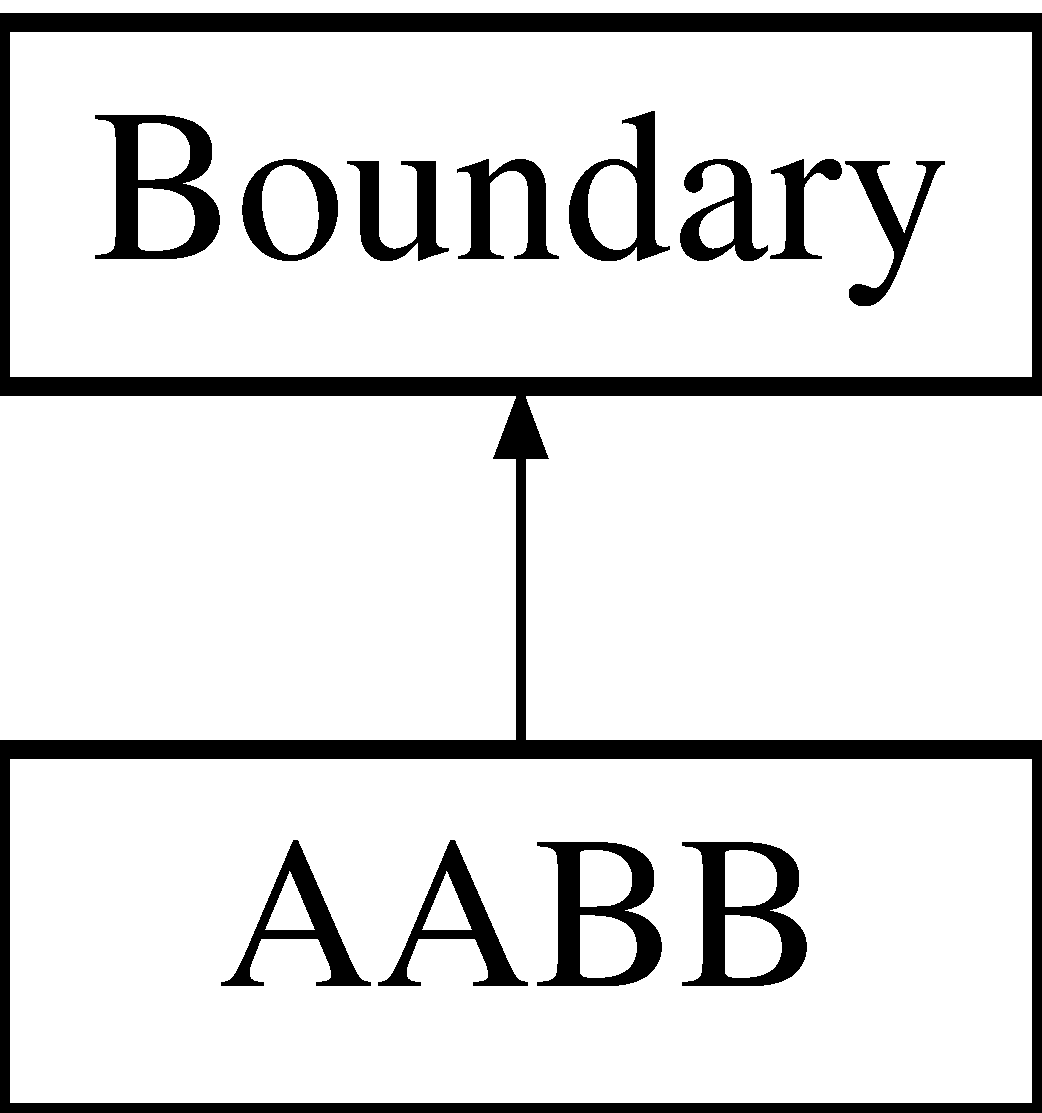
\includegraphics[height=2.000000cm]{class_a_a_b_b}
\end{center}
\end{figure}
\subsection*{Public Member Functions}
\begin{DoxyCompactItemize}
\item 
\mbox{\Hypertarget{class_a_a_b_b_a12dd0a1fb58f12ee747de9783fcc159f}\label{class_a_a_b_b_a12dd0a1fb58f12ee747de9783fcc159f}} 
{\bfseries A\+A\+BB} (\mbox{\hyperlink{class_vector3}{Vector3F}} minimum, \mbox{\hyperlink{class_vector3}{Vector3F}} maximum)
\item 
\mbox{\Hypertarget{class_a_a_b_b_ab75eda9fd4f38373f45b7cf7220e2601}\label{class_a_a_b_b_ab75eda9fd4f38373f45b7cf7220e2601}} 
{\bfseries A\+A\+BB} (const \mbox{\hyperlink{class_a_a_b_b}{A\+A\+BB}} \&copy)=default
\item 
\mbox{\Hypertarget{class_a_a_b_b_a72cb5a605e743890dcbd31f6bf32fd1e}\label{class_a_a_b_b_a72cb5a605e743890dcbd31f6bf32fd1e}} 
{\bfseries A\+A\+BB} (\mbox{\hyperlink{class_a_a_b_b}{A\+A\+BB}} \&\&move)=default
\item 
\mbox{\Hypertarget{class_a_a_b_b_a5dbdefebe25321ec24ac97d163898596}\label{class_a_a_b_b_a5dbdefebe25321ec24ac97d163898596}} 
\mbox{\hyperlink{class_a_a_b_b}{A\+A\+BB}} \& {\bfseries operator=} (const \mbox{\hyperlink{class_a_a_b_b}{A\+A\+BB}} \&rhs)=default
\item 
\mbox{\Hypertarget{class_a_a_b_b_a4d2bc2fc98412ad6160c4104f0aeb983}\label{class_a_a_b_b_a4d2bc2fc98412ad6160c4104f0aeb983}} 
const \mbox{\hyperlink{class_vector3}{Vector3F}} \& {\bfseries get\+\_\+minimum} () const
\item 
\mbox{\Hypertarget{class_a_a_b_b_a79e383c8e3010cdd1134aca704de030b}\label{class_a_a_b_b_a79e383c8e3010cdd1134aca704de030b}} 
const \mbox{\hyperlink{class_vector3}{Vector3F}} \& {\bfseries get\+\_\+maximum} () const
\item 
\mbox{\Hypertarget{class_a_a_b_b_a9c1cca9c55355340fffd6b4f707dd70d}\label{class_a_a_b_b_a9c1cca9c55355340fffd6b4f707dd70d}} 
bool {\bfseries intersects} (const \mbox{\hyperlink{class_a_a_b_b}{A\+A\+BB}} \&rhs) const
\item 
\mbox{\Hypertarget{class_a_a_b_b_ad517489d4c7a73d99ca28b126283daf0}\label{class_a_a_b_b_ad517489d4c7a73d99ca28b126283daf0}} 
bool {\bfseries intersects} (const \mbox{\hyperlink{class_vector3}{Vector3F}} \&point) const
\item 
virtual bool \mbox{\hyperlink{class_a_a_b_b_ab427a4455732a16802103e06ed4af02a}{intersects}} (\mbox{\hyperlink{class_boundary}{Boundary}} $\ast$other\+\_\+boundary) const override
\end{DoxyCompactItemize}


\subsection{Detailed Description}
Axis-\/\+Aligned Bounding-\/\+Box. Very lightweight but is a very limited and minimalistic box-\/shaped boundary for an object. Use if performance $>$ precision. 

\subsection{Member Function Documentation}
\mbox{\Hypertarget{class_a_a_b_b_ab427a4455732a16802103e06ed4af02a}\label{class_a_a_b_b_ab427a4455732a16802103e06ed4af02a}} 
\index{A\+A\+BB@{A\+A\+BB}!intersects@{intersects}}
\index{intersects@{intersects}!A\+A\+BB@{A\+A\+BB}}
\subsubsection{\texorpdfstring{intersects()}{intersects()}}
{\footnotesize\ttfamily bool A\+A\+B\+B\+::intersects (\begin{DoxyParamCaption}\item[{\mbox{\hyperlink{class_boundary}{Boundary}} $\ast$}]{other\+\_\+boundary }\end{DoxyParamCaption}) const\hspace{0.3cm}{\ttfamily [override]}, {\ttfamily [virtual]}}

Pure virtual. Override this if you want to make your own Boundaries. 

Implements \mbox{\hyperlink{class_boundary_a364909bdfa4a4945f974c34a39e198cc}{Boundary}}.



The documentation for this class was generated from the following files\+:\begin{DoxyCompactItemize}
\item 
src/physics/boundary.\+hpp\item 
src/physics/boundary.\+cpp\end{DoxyCompactItemize}

\hypertarget{class_audio_clip}{}\section{Audio\+Clip Class Reference}
\label{class_audio_clip}\index{Audio\+Clip@{Audio\+Clip}}


{\ttfamily \#include $<$audio.\+hpp$>$}

Inheritance diagram for Audio\+Clip\+:\begin{figure}[H]
\begin{center}
\leavevmode
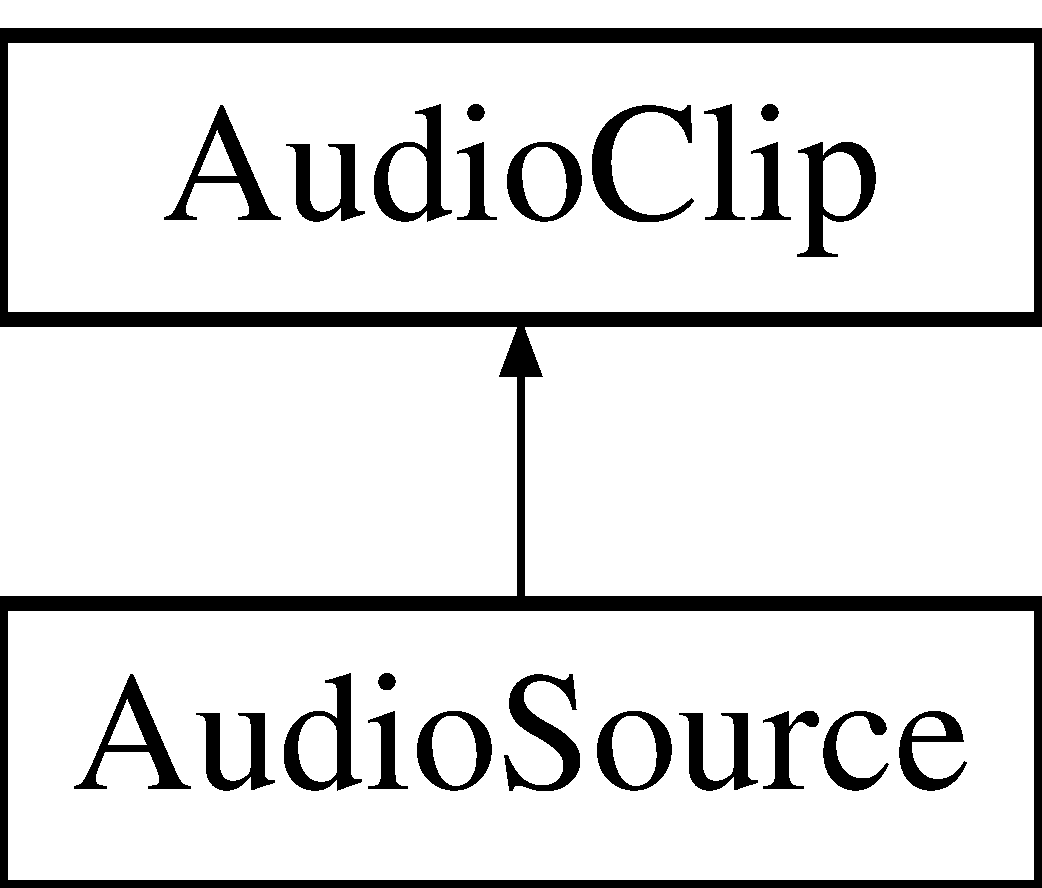
\includegraphics[height=2.000000cm]{class_audio_clip}
\end{center}
\end{figure}
\subsection*{Public Member Functions}
\begin{DoxyCompactItemize}
\item 
\mbox{\hyperlink{class_audio_clip_a92cb3dceab020f54290b05b1ae5de974}{Audio\+Clip}} (std\+::string filename)
\item 
\mbox{\hyperlink{class_audio_clip_ac5664fc84d17e5e31c1daacdec89b3cf}{Audio\+Clip}} (const \mbox{\hyperlink{class_audio_clip}{Audio\+Clip}} \&copy)
\item 
\mbox{\hyperlink{class_audio_clip_a0a4d351823548e0f54625c37db221c82}{Audio\+Clip}} (\mbox{\hyperlink{class_audio_clip}{Audio\+Clip}} \&\&move)
\item 
virtual \mbox{\hyperlink{class_audio_clip_ab929796e463c51c50f2ad4e9acec35da}{$\sim$\+Audio\+Clip}} ()
\item 
\mbox{\Hypertarget{class_audio_clip_ac1466d6ec65150fa8beb08611cda995c}\label{class_audio_clip_ac1466d6ec65150fa8beb08611cda995c}} 
\mbox{\hyperlink{class_audio_clip}{Audio\+Clip}} \& {\bfseries operator=} (const \mbox{\hyperlink{class_audio_clip}{Audio\+Clip}} \&rhs)=delete
\item 
void \mbox{\hyperlink{class_audio_clip_a615c3e8e6da9cdf8b98c1682135c2a75}{play}} ()
\item 
\mbox{\Hypertarget{class_audio_clip_a86486cb3622e9056d4d5f580889f9f16}\label{class_audio_clip_a86486cb3622e9056d4d5f580889f9f16}} 
int {\bfseries get\+\_\+channel} () const
\item 
\mbox{\Hypertarget{class_audio_clip_ae4ff05317126ce507a64c836f524ca4f}\label{class_audio_clip_ae4ff05317126ce507a64c836f524ca4f}} 
Uint32 {\bfseries get\+\_\+audio\+\_\+length} () const
\item 
\mbox{\Hypertarget{class_audio_clip_aadb9a7b1a085647f61f0120953734ca0}\label{class_audio_clip_aadb9a7b1a085647f61f0120953734ca0}} 
const std\+::string \& {\bfseries get\+\_\+file\+\_\+name} () const
\end{DoxyCompactItemize}


\subsection{Detailed Description}
Playable audio file. Use this for short audio segments like sound effects. 

\subsection{Constructor \& Destructor Documentation}
\mbox{\Hypertarget{class_audio_clip_a92cb3dceab020f54290b05b1ae5de974}\label{class_audio_clip_a92cb3dceab020f54290b05b1ae5de974}} 
\index{Audio\+Clip@{Audio\+Clip}!Audio\+Clip@{Audio\+Clip}}
\index{Audio\+Clip@{Audio\+Clip}!Audio\+Clip@{Audio\+Clip}}
\subsubsection{\texorpdfstring{Audio\+Clip()}{AudioClip()}\hspace{0.1cm}{\footnotesize\ttfamily [1/3]}}
{\footnotesize\ttfamily Audio\+Clip\+::\+Audio\+Clip (\begin{DoxyParamCaption}\item[{std\+::string}]{filename }\end{DoxyParamCaption})}

Load \mbox{\hyperlink{class_audio_clip}{Audio\+Clip}} from existing file (must be wavefront audio .wav) \mbox{\Hypertarget{class_audio_clip_ac5664fc84d17e5e31c1daacdec89b3cf}\label{class_audio_clip_ac5664fc84d17e5e31c1daacdec89b3cf}} 
\index{Audio\+Clip@{Audio\+Clip}!Audio\+Clip@{Audio\+Clip}}
\index{Audio\+Clip@{Audio\+Clip}!Audio\+Clip@{Audio\+Clip}}
\subsubsection{\texorpdfstring{Audio\+Clip()}{AudioClip()}\hspace{0.1cm}{\footnotesize\ttfamily [2/3]}}
{\footnotesize\ttfamily Audio\+Clip\+::\+Audio\+Clip (\begin{DoxyParamCaption}\item[{const \mbox{\hyperlink{class_audio_clip}{Audio\+Clip}} \&}]{copy }\end{DoxyParamCaption})}

Construct \mbox{\hyperlink{class_audio_clip}{Audio\+Clip}} using the filename of copy. \mbox{\Hypertarget{class_audio_clip_a0a4d351823548e0f54625c37db221c82}\label{class_audio_clip_a0a4d351823548e0f54625c37db221c82}} 
\index{Audio\+Clip@{Audio\+Clip}!Audio\+Clip@{Audio\+Clip}}
\index{Audio\+Clip@{Audio\+Clip}!Audio\+Clip@{Audio\+Clip}}
\subsubsection{\texorpdfstring{Audio\+Clip()}{AudioClip()}\hspace{0.1cm}{\footnotesize\ttfamily [3/3]}}
{\footnotesize\ttfamily Audio\+Clip\+::\+Audio\+Clip (\begin{DoxyParamCaption}\item[{\mbox{\hyperlink{class_audio_clip}{Audio\+Clip}} \&\&}]{move }\end{DoxyParamCaption})}

Construct \mbox{\hyperlink{class_audio_clip}{Audio\+Clip}} using the same chunk as move. Also copies move\textquotesingle{}s filename. \mbox{\Hypertarget{class_audio_clip_ab929796e463c51c50f2ad4e9acec35da}\label{class_audio_clip_ab929796e463c51c50f2ad4e9acec35da}} 
\index{Audio\+Clip@{Audio\+Clip}!````~Audio\+Clip@{$\sim$\+Audio\+Clip}}
\index{````~Audio\+Clip@{$\sim$\+Audio\+Clip}!Audio\+Clip@{Audio\+Clip}}
\subsubsection{\texorpdfstring{$\sim$\+Audio\+Clip()}{~AudioClip()}}
{\footnotesize\ttfamily Audio\+Clip\+::$\sim$\+Audio\+Clip (\begin{DoxyParamCaption}{ }\end{DoxyParamCaption})\hspace{0.3cm}{\ttfamily [virtual]}}

Deallocate memory from the S\+D\+L\+\_\+\+Mixer functionality. 

\subsection{Member Function Documentation}
\mbox{\Hypertarget{class_audio_clip_a615c3e8e6da9cdf8b98c1682135c2a75}\label{class_audio_clip_a615c3e8e6da9cdf8b98c1682135c2a75}} 
\index{Audio\+Clip@{Audio\+Clip}!play@{play}}
\index{play@{play}!Audio\+Clip@{Audio\+Clip}}
\subsubsection{\texorpdfstring{play()}{play()}}
{\footnotesize\ttfamily void Audio\+Clip\+::play (\begin{DoxyParamCaption}{ }\end{DoxyParamCaption})}

Plays the audio. The audio will play until either the destructor is called or the audio is finished; whichever takes place first. Note\+: Invoking tz\+::audio\+::play\+\_\+async on an instance of \mbox{\hyperlink{class_audio_clip}{Audio\+Clip}} will extend the lifetime of the instance such that the audio clip is guaranteed to be fully played. 

The documentation for this class was generated from the following files\+:\begin{DoxyCompactItemize}
\item 
src/audio/audio.\+hpp\item 
src/audio/audio.\+cpp\end{DoxyCompactItemize}

\hypertarget{class_audio_music}{}\section{Audio\+Music Class Reference}
\label{class_audio_music}\index{Audio\+Music@{Audio\+Music}}


{\ttfamily \#include $<$audio.\+hpp$>$}

\subsection*{Public Member Functions}
\begin{DoxyCompactItemize}
\item 
\mbox{\Hypertarget{class_audio_music_a260b6ddf241e3f1e865a49309aa12572}\label{class_audio_music_a260b6ddf241e3f1e865a49309aa12572}} 
{\bfseries Audio\+Music} (std\+::string filename)
\item 
\mbox{\Hypertarget{class_audio_music_a742e8a6822342b8de08175e3948e5830}\label{class_audio_music_a742e8a6822342b8de08175e3948e5830}} 
{\bfseries Audio\+Music} (const \mbox{\hyperlink{class_audio_music}{Audio\+Music}} \&copy)
\item 
\mbox{\Hypertarget{class_audio_music_a55779c2cc75a89cf808d92e313d80ae8}\label{class_audio_music_a55779c2cc75a89cf808d92e313d80ae8}} 
{\bfseries Audio\+Music} (\mbox{\hyperlink{class_audio_music}{Audio\+Music}} \&\&move)
\item 
\mbox{\Hypertarget{class_audio_music_a9487a5b790ede77cc96efd6e70322253}\label{class_audio_music_a9487a5b790ede77cc96efd6e70322253}} 
\mbox{\hyperlink{class_audio_music}{Audio\+Music}} \& {\bfseries operator=} (const \mbox{\hyperlink{class_audio_music}{Audio\+Music}} \&rhs)=delete
\item 
\mbox{\Hypertarget{class_audio_music_a794b5133068bacd9d5954316c466e781}\label{class_audio_music_a794b5133068bacd9d5954316c466e781}} 
const std\+::string \& {\bfseries get\+\_\+file\+\_\+name} () const
\item 
\mbox{\Hypertarget{class_audio_music_a103d6a71de74441ad5b63fec5f50d656}\label{class_audio_music_a103d6a71de74441ad5b63fec5f50d656}} 
bool {\bfseries is\+\_\+paused} () const
\item 
void \mbox{\hyperlink{class_audio_music_a9867971e26b4d081936287af1923fd1a}{play}} (bool priority=true) const
\item 
void \mbox{\hyperlink{class_audio_music_a5de1c2fc9f565af444c48b85b56d7c8f}{set\+\_\+paused}} (bool pause=true)
\end{DoxyCompactItemize}


\subsection{Detailed Description}
Playable audio file. Use this for longer audio segments such as background music. 

\subsection{Member Function Documentation}
\mbox{\Hypertarget{class_audio_music_a9867971e26b4d081936287af1923fd1a}\label{class_audio_music_a9867971e26b4d081936287af1923fd1a}} 
\index{Audio\+Music@{Audio\+Music}!play@{play}}
\index{play@{play}!Audio\+Music@{Audio\+Music}}
\subsubsection{\texorpdfstring{play()}{play()}}
{\footnotesize\ttfamily void Audio\+Music\+::play (\begin{DoxyParamCaption}\item[{bool}]{priority = {\ttfamily true} }\end{DoxyParamCaption}) const}

Play should be invoked only once and not to un-\/pause music. \mbox{\Hypertarget{class_audio_music_a5de1c2fc9f565af444c48b85b56d7c8f}\label{class_audio_music_a5de1c2fc9f565af444c48b85b56d7c8f}} 
\index{Audio\+Music@{Audio\+Music}!set\+\_\+paused@{set\+\_\+paused}}
\index{set\+\_\+paused@{set\+\_\+paused}!Audio\+Music@{Audio\+Music}}
\subsubsection{\texorpdfstring{set\+\_\+paused()}{set\_paused()}}
{\footnotesize\ttfamily void Audio\+Music\+::set\+\_\+paused (\begin{DoxyParamCaption}\item[{bool}]{pause = {\ttfamily true} }\end{DoxyParamCaption})}

Pause/\+Resume the music. 

The documentation for this class was generated from the following files\+:\begin{DoxyCompactItemize}
\item 
src/audio/audio.\+hpp\item 
src/audio/audio.\+cpp\end{DoxyCompactItemize}

\hypertarget{class_audio_source}{}\section{Audio\+Source Class Reference}
\label{class_audio_source}\index{Audio\+Source@{Audio\+Source}}


{\ttfamily \#include $<$audio.\+hpp$>$}

Inheritance diagram for Audio\+Source\+:\begin{figure}[H]
\begin{center}
\leavevmode
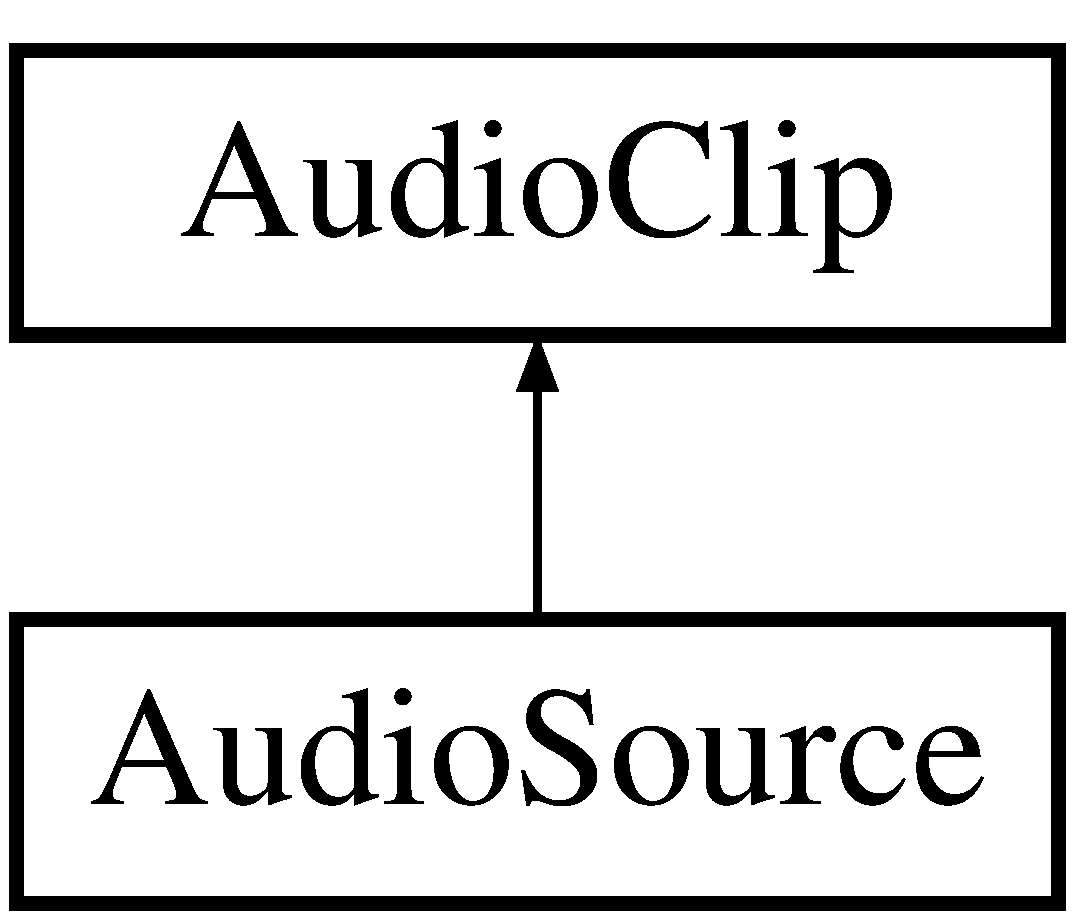
\includegraphics[height=2.000000cm]{class_audio_source}
\end{center}
\end{figure}
\subsection*{Public Member Functions}
\begin{DoxyCompactItemize}
\item 
\mbox{\Hypertarget{class_audio_source_a0cb3b38b2e113d9b8b86b4d9fd8046d8}\label{class_audio_source_a0cb3b38b2e113d9b8b86b4d9fd8046d8}} 
{\bfseries Audio\+Source} (std\+::string filename)
\item 
\mbox{\Hypertarget{class_audio_source_a238c56998543c1bbe08d67467957e050}\label{class_audio_source_a238c56998543c1bbe08d67467957e050}} 
{\bfseries Audio\+Source} (const \mbox{\hyperlink{class_audio_source}{Audio\+Source}} \&copy)=default
\item 
\mbox{\Hypertarget{class_audio_source_a9ff96d14841ecd4aef40918cf8348464}\label{class_audio_source_a9ff96d14841ecd4aef40918cf8348464}} 
{\bfseries Audio\+Source} (\mbox{\hyperlink{class_audio_source}{Audio\+Source}} \&\&move)=default
\item 
\mbox{\Hypertarget{class_audio_source_aa73e35b3259f93e55a897b4c42e198d8}\label{class_audio_source_aa73e35b3259f93e55a897b4c42e198d8}} 
\mbox{\hyperlink{class_audio_source}{Audio\+Source}} \& {\bfseries operator=} (const \mbox{\hyperlink{class_audio_source}{Audio\+Source}} \&rhs)=delete
\item 
void \mbox{\hyperlink{class_audio_source_acc045186f5f7516c3b71598f0b65b0c5}{update}} (const \mbox{\hyperlink{class_vector3}{Vector3F}} \&source\+\_\+position, const \mbox{\hyperlink{class_camera}{Camera}} \&relative\+\_\+to) const
\end{DoxyCompactItemize}


\subsection{Detailed Description}
Playable audio file, but from a position in 3D space. Same properties as \mbox{\hyperlink{class_audio_clip}{Audio\+Clip}}. 

\subsection{Member Function Documentation}
\mbox{\Hypertarget{class_audio_source_acc045186f5f7516c3b71598f0b65b0c5}\label{class_audio_source_acc045186f5f7516c3b71598f0b65b0c5}} 
\index{Audio\+Source@{Audio\+Source}!update@{update}}
\index{update@{update}!Audio\+Source@{Audio\+Source}}
\subsubsection{\texorpdfstring{update()}{update()}}
{\footnotesize\ttfamily void Audio\+Source\+::update (\begin{DoxyParamCaption}\item[{const \mbox{\hyperlink{class_vector3}{Vector3F}} \&}]{source\+\_\+position,  }\item[{const \mbox{\hyperlink{class_camera}{Camera}} \&}]{relative\+\_\+to }\end{DoxyParamCaption}) const}

Should be invoked whenever the camera rotates or moves or the \mbox{\hyperlink{class_audio_source}{Audio\+Source}} position is changed. 

The documentation for this class was generated from the following files\+:\begin{DoxyCompactItemize}
\item 
src/audio/audio.\+hpp\item 
src/audio/audio.\+cpp\end{DoxyCompactItemize}

\hypertarget{class_bitmap}{}\section{Bitmap$<$ Pixel $>$ Class Template Reference}
\label{class_bitmap}\index{Bitmap$<$ Pixel $>$@{Bitmap$<$ Pixel $>$}}


{\ttfamily \#include $<$graphics.\+hpp$>$}

\subsection*{Public Member Functions}
\begin{DoxyCompactItemize}
\item 
\mbox{\hyperlink{class_bitmap_a58c9612034bf712ac71d92951c950ff5}{Bitmap}} (std\+::vector$<$ Pixel $>$ \mbox{\hyperlink{class_bitmap_acd003dbe23a69571311e6be4149eca51}{pixels}}=std\+::vector$<$ Pixel $>$(), int \mbox{\hyperlink{class_bitmap_a8733772b70b8971d11e3eb4eec6970a0}{width}}=0, int \mbox{\hyperlink{class_bitmap_a307fcc931419962f442ea32139e75a0b}{height}}=0)
\end{DoxyCompactItemize}
\subsection*{Public Attributes}
\begin{DoxyCompactItemize}
\item 
\mbox{\Hypertarget{class_bitmap_acd003dbe23a69571311e6be4149eca51}\label{class_bitmap_acd003dbe23a69571311e6be4149eca51}} 
std\+::vector$<$ Pixel $>$ \mbox{\hyperlink{class_bitmap_acd003dbe23a69571311e6be4149eca51}{pixels}}
\begin{DoxyCompactList}\small\item\em Container for all pixels. \end{DoxyCompactList}\item 
\mbox{\Hypertarget{class_bitmap_a8733772b70b8971d11e3eb4eec6970a0}\label{class_bitmap_a8733772b70b8971d11e3eb4eec6970a0}} 
int \mbox{\hyperlink{class_bitmap_a8733772b70b8971d11e3eb4eec6970a0}{width}}
\begin{DoxyCompactList}\small\item\em Width of the \mbox{\hyperlink{class_bitmap}{Bitmap}}, in pixels. \end{DoxyCompactList}\item 
\mbox{\Hypertarget{class_bitmap_a307fcc931419962f442ea32139e75a0b}\label{class_bitmap_a307fcc931419962f442ea32139e75a0b}} 
int \mbox{\hyperlink{class_bitmap_a307fcc931419962f442ea32139e75a0b}{height}}
\begin{DoxyCompactList}\small\item\em Height of the \mbox{\hyperlink{class_bitmap}{Bitmap}}, in pixels. \end{DoxyCompactList}\end{DoxyCompactItemize}


\subsection{Detailed Description}
\subsubsection*{template$<$class Pixel = Pixel\+R\+G\+BA$>$\newline
class Bitmap$<$ Pixel $>$}

\mbox{\hyperlink{class_bitmap}{Bitmap}} representing Pixel data in any format. Topaz uses \mbox{\hyperlink{class_pixel_r_g_b_a}{Pixel\+R\+G\+BA}} as the template parameter, but you may provide any valid class with a public Vector4$<$\+T$>$ called \textquotesingle{}data\textquotesingle{}. 

\subsection{Constructor \& Destructor Documentation}
\mbox{\Hypertarget{class_bitmap_a58c9612034bf712ac71d92951c950ff5}\label{class_bitmap_a58c9612034bf712ac71d92951c950ff5}} 
\index{Bitmap@{Bitmap}!Bitmap@{Bitmap}}
\index{Bitmap@{Bitmap}!Bitmap@{Bitmap}}
\subsubsection{\texorpdfstring{Bitmap()}{Bitmap()}}
{\footnotesize\ttfamily template$<$class Pixel = Pixel\+R\+G\+BA$>$ \\
\mbox{\hyperlink{class_bitmap}{Bitmap}}$<$ Pixel $>$\+::\mbox{\hyperlink{class_bitmap}{Bitmap}} (\begin{DoxyParamCaption}\item[{std\+::vector$<$ Pixel $>$}]{pixels = {\ttfamily std\+:\+:vector$<$Pixel$>$()},  }\item[{int}]{width = {\ttfamily 0},  }\item[{int}]{height = {\ttfamily 0} }\end{DoxyParamCaption})\hspace{0.3cm}{\ttfamily [inline]}}

Construct a \mbox{\hyperlink{class_bitmap}{Bitmap}} directly from a vector of Pixels. 
\begin{DoxyParams}{Parameters}
{\em pixels} & -\/ Pixel data to construct the bitmap. \\
\hline
{\em width} & -\/ Width of the bitmap, in pixels. \\
\hline
{\em height} & -\/ Height of the bitmap, in pixels. \\
\hline
\end{DoxyParams}


The documentation for this class was generated from the following file\+:\begin{DoxyCompactItemize}
\item 
src/graphics/graphics.\+hpp\end{DoxyCompactItemize}

\hypertarget{class_boundary}{}\section{Boundary Class Reference}
\label{class_boundary}\index{Boundary@{Boundary}}


{\ttfamily \#include $<$boundary.\+hpp$>$}

Inheritance diagram for Boundary\+:\begin{figure}[H]
\begin{center}
\leavevmode
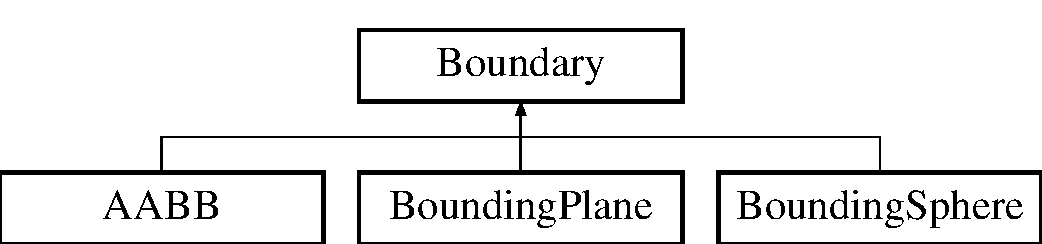
\includegraphics[height=2.000000cm]{class_boundary}
\end{center}
\end{figure}
\subsection*{Public Member Functions}
\begin{DoxyCompactItemize}
\item 
\mbox{\Hypertarget{class_boundary_a1c95b0fe70da9152d4a6c125cb424973}\label{class_boundary_a1c95b0fe70da9152d4a6c125cb424973}} 
{\bfseries Boundary} (const \mbox{\hyperlink{class_boundary}{Boundary}} \&copy)=default
\item 
\mbox{\Hypertarget{class_boundary_adca3ef87d10d6f79ec68ee2489498907}\label{class_boundary_adca3ef87d10d6f79ec68ee2489498907}} 
{\bfseries Boundary} (\mbox{\hyperlink{class_boundary}{Boundary}} \&\&move)=default
\item 
\mbox{\Hypertarget{class_boundary_a2028692d79f9c89bfe6232147d282991}\label{class_boundary_a2028692d79f9c89bfe6232147d282991}} 
\mbox{\hyperlink{class_boundary}{Boundary}} \& {\bfseries operator=} (const \mbox{\hyperlink{class_boundary}{Boundary}} \&rhs)=default
\item 
virtual bool \mbox{\hyperlink{class_boundary_a364909bdfa4a4945f974c34a39e198cc}{intersects}} (\mbox{\hyperlink{class_boundary}{Boundary}} $\ast$other\+\_\+boundary) const =0
\end{DoxyCompactItemize}


\subsection{Detailed Description}
Abstract. Not available for non-\/polymorphic use. Inherit from this to create custom boundaries. Represents a simple boundary in space. 

\subsection{Member Function Documentation}
\mbox{\Hypertarget{class_boundary_a364909bdfa4a4945f974c34a39e198cc}\label{class_boundary_a364909bdfa4a4945f974c34a39e198cc}} 
\index{Boundary@{Boundary}!intersects@{intersects}}
\index{intersects@{intersects}!Boundary@{Boundary}}
\subsubsection{\texorpdfstring{intersects()}{intersects()}}
{\footnotesize\ttfamily virtual bool Boundary\+::intersects (\begin{DoxyParamCaption}\item[{\mbox{\hyperlink{class_boundary}{Boundary}} $\ast$}]{other\+\_\+boundary }\end{DoxyParamCaption}) const\hspace{0.3cm}{\ttfamily [pure virtual]}}

Pure virtual. Override this if you want to make your own Boundaries. 

Implemented in \mbox{\hyperlink{class_bounding_plane_a3d956121121f32384cab3cab34544d6e}{Bounding\+Plane}}, \mbox{\hyperlink{class_a_a_b_b_ab427a4455732a16802103e06ed4af02a}{A\+A\+BB}}, and \mbox{\hyperlink{class_bounding_sphere_aab64d759fac6a9835ac24d6fca8530d6}{Bounding\+Sphere}}.



The documentation for this class was generated from the following file\+:\begin{DoxyCompactItemize}
\item 
src/physics/boundary.\+hpp\end{DoxyCompactItemize}

\hypertarget{class_bounding_plane}{}\section{Bounding\+Plane Class Reference}
\label{class_bounding_plane}\index{Bounding\+Plane@{Bounding\+Plane}}


{\ttfamily \#include $<$boundary.\+hpp$>$}

Inheritance diagram for Bounding\+Plane\+:\begin{figure}[H]
\begin{center}
\leavevmode
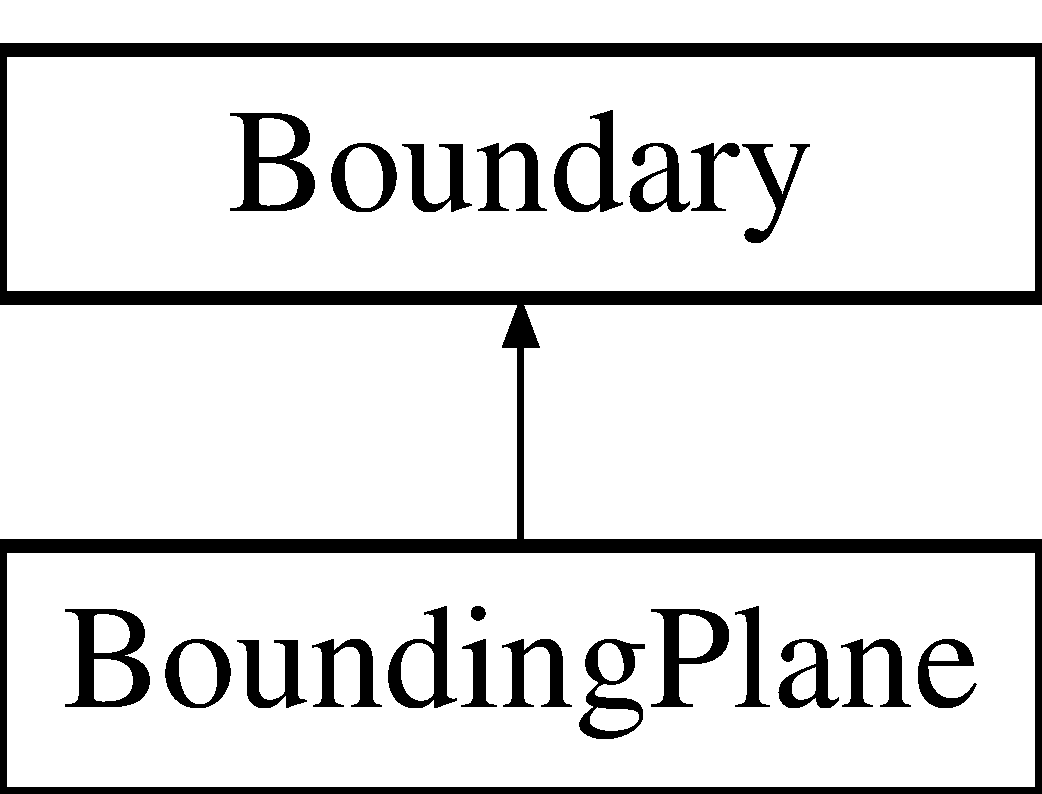
\includegraphics[height=2.000000cm]{class_bounding_plane}
\end{center}
\end{figure}
\subsection*{Public Member Functions}
\begin{DoxyCompactItemize}
\item 
\mbox{\Hypertarget{class_bounding_plane_a8d0f14beb814c929ed3322b22f662917}\label{class_bounding_plane_a8d0f14beb814c929ed3322b22f662917}} 
{\bfseries Bounding\+Plane} (\mbox{\hyperlink{class_vector3}{Vector3F}} normal, float distance)
\item 
\mbox{\Hypertarget{class_bounding_plane_a007cc683824c23bc818b2f3584ce5386}\label{class_bounding_plane_a007cc683824c23bc818b2f3584ce5386}} 
{\bfseries Bounding\+Plane} (const \mbox{\hyperlink{class_bounding_plane}{Bounding\+Plane}} \&copy)=default
\item 
\mbox{\Hypertarget{class_bounding_plane_af1db7dfae2ab49d62f73eb7db3f39e29}\label{class_bounding_plane_af1db7dfae2ab49d62f73eb7db3f39e29}} 
{\bfseries Bounding\+Plane} (\mbox{\hyperlink{class_bounding_plane}{Bounding\+Plane}} \&\&move)=default
\item 
\mbox{\Hypertarget{class_bounding_plane_adbb48a97748ef40bb761a2018f1d2473}\label{class_bounding_plane_adbb48a97748ef40bb761a2018f1d2473}} 
\mbox{\hyperlink{class_bounding_plane}{Bounding\+Plane}} \& {\bfseries operator=} (const \mbox{\hyperlink{class_bounding_plane}{Bounding\+Plane}} \&rhs)=default
\item 
\mbox{\Hypertarget{class_bounding_plane_a7c656534126a09de2768bffe9cdc5964}\label{class_bounding_plane_a7c656534126a09de2768bffe9cdc5964}} 
const \mbox{\hyperlink{class_vector3}{Vector3F}} \& {\bfseries get\+\_\+normal} () const
\item 
\mbox{\Hypertarget{class_bounding_plane_ac34d406c0f223d599a7b7aad49d4cb54}\label{class_bounding_plane_ac34d406c0f223d599a7b7aad49d4cb54}} 
float {\bfseries get\+\_\+distance} () const
\item 
\mbox{\Hypertarget{class_bounding_plane_aa271e305ed07117a8c82eedf1fd0f037}\label{class_bounding_plane_aa271e305ed07117a8c82eedf1fd0f037}} 
\mbox{\hyperlink{class_bounding_plane}{Bounding\+Plane}} {\bfseries normalised} () const
\item 
\mbox{\Hypertarget{class_bounding_plane_af55931eb0667bcfaa91db85abcddc7a6}\label{class_bounding_plane_af55931eb0667bcfaa91db85abcddc7a6}} 
bool {\bfseries intersects} (const \mbox{\hyperlink{class_bounding_sphere}{Bounding\+Sphere}} \&other) const
\item 
virtual bool \mbox{\hyperlink{class_bounding_plane_a3d956121121f32384cab3cab34544d6e}{intersects}} (\mbox{\hyperlink{class_boundary}{Boundary}} $\ast$other\+\_\+boundary) const override
\end{DoxyCompactItemize}


\subsection{Detailed Description}
Used to bound planes. Useful for objects such as walls or floors. 

\subsection{Member Function Documentation}
\mbox{\Hypertarget{class_bounding_plane_a3d956121121f32384cab3cab34544d6e}\label{class_bounding_plane_a3d956121121f32384cab3cab34544d6e}} 
\index{Bounding\+Plane@{Bounding\+Plane}!intersects@{intersects}}
\index{intersects@{intersects}!Bounding\+Plane@{Bounding\+Plane}}
\subsubsection{\texorpdfstring{intersects()}{intersects()}}
{\footnotesize\ttfamily virtual bool Bounding\+Plane\+::intersects (\begin{DoxyParamCaption}\item[{\mbox{\hyperlink{class_boundary}{Boundary}} $\ast$}]{other\+\_\+boundary }\end{DoxyParamCaption}) const\hspace{0.3cm}{\ttfamily [override]}, {\ttfamily [virtual]}}

Pure virtual. Override this if you want to make your own Boundaries. 

Implements \mbox{\hyperlink{class_boundary_a364909bdfa4a4945f974c34a39e198cc}{Boundary}}.



The documentation for this class was generated from the following files\+:\begin{DoxyCompactItemize}
\item 
src/physics/boundary.\+hpp\item 
src/physics/boundary.\+cpp\end{DoxyCompactItemize}

\hypertarget{class_bounding_sphere}{}\section{Bounding\+Sphere Class Reference}
\label{class_bounding_sphere}\index{Bounding\+Sphere@{Bounding\+Sphere}}


{\ttfamily \#include $<$boundary.\+hpp$>$}

Inheritance diagram for Bounding\+Sphere\+:\begin{figure}[H]
\begin{center}
\leavevmode
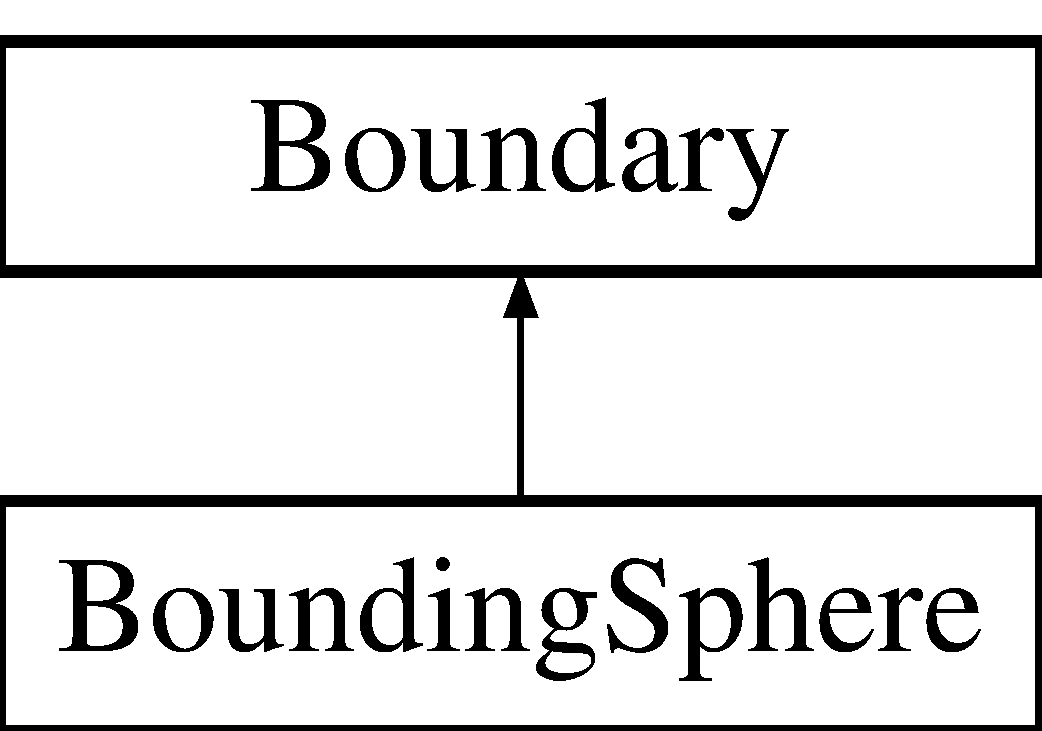
\includegraphics[height=2.000000cm]{class_bounding_sphere}
\end{center}
\end{figure}
\subsection*{Public Member Functions}
\begin{DoxyCompactItemize}
\item 
\mbox{\Hypertarget{class_bounding_sphere_a9d6fd19a13a3ec6106254640591a26b8}\label{class_bounding_sphere_a9d6fd19a13a3ec6106254640591a26b8}} 
{\bfseries Bounding\+Sphere} (\mbox{\hyperlink{class_vector3}{Vector3F}} centre, float radius)
\item 
\mbox{\Hypertarget{class_bounding_sphere_a7c9b518f0f0a9656e9efa861f5e6ee9d}\label{class_bounding_sphere_a7c9b518f0f0a9656e9efa861f5e6ee9d}} 
{\bfseries Bounding\+Sphere} (const \mbox{\hyperlink{class_bounding_sphere}{Bounding\+Sphere}} \&copy)=default
\item 
\mbox{\Hypertarget{class_bounding_sphere_a1f5065e1481dcfd002a50b5fed5f5e6a}\label{class_bounding_sphere_a1f5065e1481dcfd002a50b5fed5f5e6a}} 
{\bfseries Bounding\+Sphere} (\mbox{\hyperlink{class_bounding_sphere}{Bounding\+Sphere}} \&\&move)=default
\item 
\mbox{\Hypertarget{class_bounding_sphere_ad77f5db8cff86f6009e0d23604b912f3}\label{class_bounding_sphere_ad77f5db8cff86f6009e0d23604b912f3}} 
\mbox{\hyperlink{class_bounding_sphere}{Bounding\+Sphere}} \& {\bfseries operator=} (const \mbox{\hyperlink{class_bounding_sphere}{Bounding\+Sphere}} \&rhs)=default
\item 
\mbox{\Hypertarget{class_bounding_sphere_a8d81f5c646d752821c356742819ff512}\label{class_bounding_sphere_a8d81f5c646d752821c356742819ff512}} 
const \mbox{\hyperlink{class_vector3}{Vector3F}} \& {\bfseries get\+\_\+centre} () const
\item 
\mbox{\Hypertarget{class_bounding_sphere_a5049afba6967afbd35f3e18d82a51acd}\label{class_bounding_sphere_a5049afba6967afbd35f3e18d82a51acd}} 
float {\bfseries get\+\_\+radius} () const
\item 
\mbox{\Hypertarget{class_bounding_sphere_aea072dbeaec73a4738dd7adf496a11ae}\label{class_bounding_sphere_aea072dbeaec73a4738dd7adf496a11ae}} 
bool {\bfseries intersects} (const \mbox{\hyperlink{class_bounding_sphere}{Bounding\+Sphere}} \&rhs) const
\item 
virtual bool \mbox{\hyperlink{class_bounding_sphere_aab64d759fac6a9835ac24d6fca8530d6}{intersects}} (\mbox{\hyperlink{class_boundary}{Boundary}} $\ast$other\+\_\+boundary) const override
\end{DoxyCompactItemize}


\subsection{Detailed Description}
Used to bound physical spherical shapes in 3D space. 

\subsection{Member Function Documentation}
\mbox{\Hypertarget{class_bounding_sphere_aab64d759fac6a9835ac24d6fca8530d6}\label{class_bounding_sphere_aab64d759fac6a9835ac24d6fca8530d6}} 
\index{Bounding\+Sphere@{Bounding\+Sphere}!intersects@{intersects}}
\index{intersects@{intersects}!Bounding\+Sphere@{Bounding\+Sphere}}
\subsubsection{\texorpdfstring{intersects()}{intersects()}}
{\footnotesize\ttfamily bool Bounding\+Sphere\+::intersects (\begin{DoxyParamCaption}\item[{\mbox{\hyperlink{class_boundary}{Boundary}} $\ast$}]{other\+\_\+boundary }\end{DoxyParamCaption}) const\hspace{0.3cm}{\ttfamily [override]}, {\ttfamily [virtual]}}

Pure virtual. Override this if you want to make your own Boundaries. 

Implements \mbox{\hyperlink{class_boundary_a364909bdfa4a4945f974c34a39e198cc}{Boundary}}.



The documentation for this class was generated from the following files\+:\begin{DoxyCompactItemize}
\item 
src/physics/boundary.\+hpp\item 
src/physics/boundary.\+cpp\end{DoxyCompactItemize}

\hypertarget{class_button}{}\section{Button Class Reference}
\label{class_button}\index{Button@{Button}}


{\ttfamily \#include $<$gui\+\_\+widget.\+hpp$>$}

Inheritance diagram for Button\+:\begin{figure}[H]
\begin{center}
\leavevmode
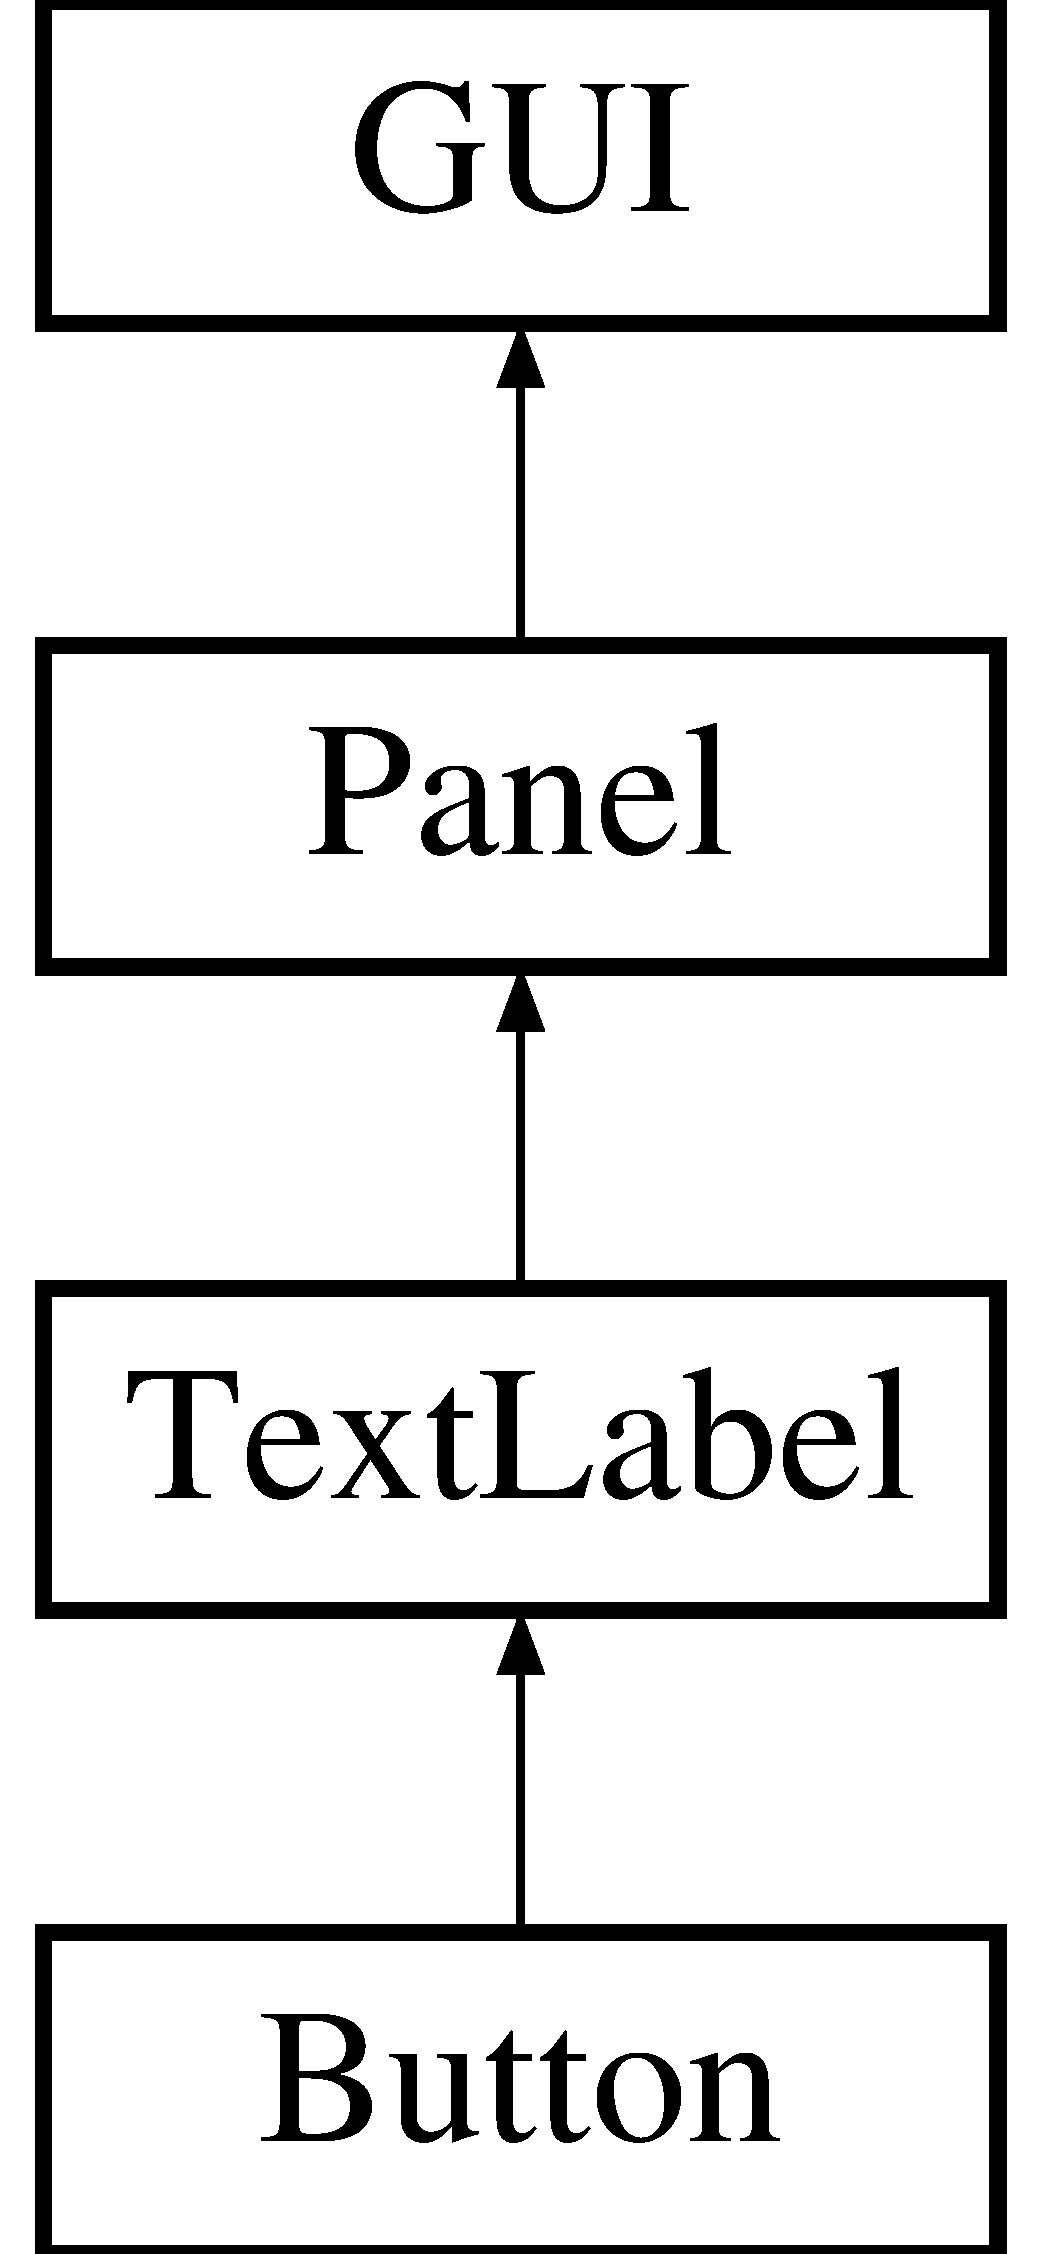
\includegraphics[height=4.000000cm]{class_button}
\end{center}
\end{figure}
\subsection*{Public Member Functions}
\begin{DoxyCompactItemize}
\item 
\mbox{\hyperlink{class_button_a228b18e1d494f3d443d9a42ad16d5568}{Button}} (float \mbox{\hyperlink{class_g_u_i_a7fa193a8ffb27bbb3bcc225e36f6d54d}{x}}, float \mbox{\hyperlink{class_g_u_i_a98f204f99ffc5ff6cffc9340bbb8c29b}{y}}, \mbox{\hyperlink{class_vector4}{Vector4F}} \mbox{\hyperlink{class_panel_a7c38e08ad80eb9972428450fb639bf66}{colour}}, std\+::optional$<$ \mbox{\hyperlink{class_vector4}{Vector4F}} $>$ background\+\_\+colour, std\+::optional$<$ \mbox{\hyperlink{class_vector3}{Vector3F}} $>$ text\+\_\+border\+\_\+colour, \mbox{\hyperlink{class_font}{Font}} font, const std\+::string \&text, \mbox{\hyperlink{class_shader}{Shader}} \&\mbox{\hyperlink{class_g_u_i_a64b007b31d0ec8a8704f9ab3bb2a7d3d}{shader}}, \mbox{\hyperlink{class_mouse_listener}{Mouse\+Listener}} \&\mbox{\hyperlink{class_button_aab6aafaa6740925acb9c69c62f68aa7e}{mouse\+\_\+listener}})
\item 
virtual void \mbox{\hyperlink{class_button_abda97f1ae8e081da3dbd0b77a27cad9d}{update}} () override
\item 
virtual bool \mbox{\hyperlink{class_button_a2c1b0adeb2920b394fe4f38354ae6604}{focused}} () const override
\item 
virtual bool \mbox{\hyperlink{class_button_aa2b16ae30fe74f215aa79c699bbf8510}{is\+\_\+mouse\+\_\+sensitive}} () const override
\item 
\mbox{\hyperlink{class_command}{Command}} $\ast$ \mbox{\hyperlink{class_button_a3f9b964049bde58b8f39170ce8b6fa2e}{get\+\_\+on\+\_\+mouse\+\_\+over}} () const
\item 
\mbox{\hyperlink{class_command}{Command}} $\ast$ \mbox{\hyperlink{class_button_ac2a5c2151dc48940ac2e9c5f07c8dd6a}{get\+\_\+on\+\_\+mouse\+\_\+click}} () const
\item 
void \mbox{\hyperlink{class_button_a6133f9b42ae1192df54babd19dec9b80}{set\+\_\+on\+\_\+mouse\+\_\+over}} (\mbox{\hyperlink{class_command}{Command}} $\ast$cmd)
\item 
void \mbox{\hyperlink{class_button_a7b60123b8609254c811e3c3cc9d50d07}{set\+\_\+on\+\_\+mouse\+\_\+click}} (\mbox{\hyperlink{class_command}{Command}} $\ast$cmd)
\item 
bool \mbox{\hyperlink{class_button_a683998d86b16a7bf4196f3f59b134f95}{moused\+\_\+over}} () const
\item 
bool \mbox{\hyperlink{class_button_a650782c10937ce67bb99aed737cd4ba1}{clicked\+\_\+on}} () const
\end{DoxyCompactItemize}
\subsection*{Protected Attributes}
\begin{DoxyCompactItemize}
\item 
\mbox{\Hypertarget{class_button_aab6aafaa6740925acb9c69c62f68aa7e}\label{class_button_aab6aafaa6740925acb9c69c62f68aa7e}} 
\mbox{\hyperlink{class_mouse_listener}{Mouse\+Listener}} \& \mbox{\hyperlink{class_button_aab6aafaa6740925acb9c69c62f68aa7e}{mouse\+\_\+listener}}
\begin{DoxyCompactList}\small\item\em \mbox{\hyperlink{class_mouse_listener}{Mouse\+Listener}} to control mouse events. \end{DoxyCompactList}\item 
\mbox{\Hypertarget{class_button_a004237b359d7783fdfa3c7fc132dcd11}\label{class_button_a004237b359d7783fdfa3c7fc132dcd11}} 
bool \mbox{\hyperlink{class_button_a004237b359d7783fdfa3c7fc132dcd11}{just\+\_\+clicked}}
\begin{DoxyCompactList}\small\item\em Stores whether the \mbox{\hyperlink{class_button}{Button}} was clicked last frame. \end{DoxyCompactList}\item 
\mbox{\Hypertarget{class_button_a14e3262785a4dea5cded2c6542c09f2b}\label{class_button_a14e3262785a4dea5cded2c6542c09f2b}} 
bool \mbox{\hyperlink{class_button_a14e3262785a4dea5cded2c6542c09f2b}{just\+\_\+moused\+\_\+over}}
\begin{DoxyCompactList}\small\item\em Stores whether the \mbox{\hyperlink{class_button}{Button}} was moused-\/over last frame. \end{DoxyCompactList}\end{DoxyCompactItemize}
\subsection*{Additional Inherited Members}


\subsection{Detailed Description}
Just like a \mbox{\hyperlink{class_text_label}{Text\+Label}}, but also is mouse-\/sensitive and pressable to execute a command. 

\subsection{Constructor \& Destructor Documentation}
\mbox{\Hypertarget{class_button_a228b18e1d494f3d443d9a42ad16d5568}\label{class_button_a228b18e1d494f3d443d9a42ad16d5568}} 
\index{Button@{Button}!Button@{Button}}
\index{Button@{Button}!Button@{Button}}
\subsubsection{\texorpdfstring{Button()}{Button()}}
{\footnotesize\ttfamily Button\+::\+Button (\begin{DoxyParamCaption}\item[{float}]{x,  }\item[{float}]{y,  }\item[{\mbox{\hyperlink{class_vector4}{Vector4F}}}]{colour,  }\item[{std\+::optional$<$ \mbox{\hyperlink{class_vector4}{Vector4F}} $>$}]{background\+\_\+colour,  }\item[{std\+::optional$<$ \mbox{\hyperlink{class_vector3}{Vector3F}} $>$}]{text\+\_\+border\+\_\+colour,  }\item[{\mbox{\hyperlink{class_font}{Font}}}]{font,  }\item[{const std\+::string \&}]{text,  }\item[{\mbox{\hyperlink{class_shader}{Shader}} \&}]{shader,  }\item[{\mbox{\hyperlink{class_mouse_listener}{Mouse\+Listener}} \&}]{mouse\+\_\+listener }\end{DoxyParamCaption})}

Construct a \mbox{\hyperlink{class_button}{Button}} with all required specifications. 
\begin{DoxyParams}{Parameters}
{\em x} & -\/ Position of the button on the x-\/axis, in pixels. \\
\hline
{\em y} & -\/ Position of the button on the y-\/axis, in pixels. \\
\hline
{\em colour} & -\/ R\+G\+B\+A-\/coded colour of the button text \\
\hline
{\em background\+\_\+colour} & -\/ R\+G\+B\+A-\/coded colour of the button background \\
\hline
{\em text\+\_\+border\+\_\+colour} & -\/ Optional R\+G\+B\+A-\/coded colour of the button text border \\
\hline
{\em font} & -\/ \mbox{\hyperlink{class_font}{Font}} used to render the text. \\
\hline
{\em text} & -\/ String representing the text displayed on the button body. \\
\hline
{\em shader} & -\/ The shader with which to render the button. \\
\hline
{\em mouse\+\_\+listener} & -\/ The mouse-\/listener responsible for providing button-\/press and mouse-\/over events \\
\hline
\end{DoxyParams}


\subsection{Member Function Documentation}
\mbox{\Hypertarget{class_button_a650782c10937ce67bb99aed737cd4ba1}\label{class_button_a650782c10937ce67bb99aed737cd4ba1}} 
\index{Button@{Button}!clicked\+\_\+on@{clicked\+\_\+on}}
\index{clicked\+\_\+on@{clicked\+\_\+on}!Button@{Button}}
\subsubsection{\texorpdfstring{clicked\+\_\+on()}{clicked\_on()}}
{\footnotesize\ttfamily bool Button\+::clicked\+\_\+on (\begin{DoxyParamCaption}{ }\end{DoxyParamCaption}) const}

Query whether the button is currently being clicked on or not \begin{DoxyReturn}{Returns}
-\/ True if the button is being clicked on. False otherwise. 
\end{DoxyReturn}
\mbox{\Hypertarget{class_button_a2c1b0adeb2920b394fe4f38354ae6604}\label{class_button_a2c1b0adeb2920b394fe4f38354ae6604}} 
\index{Button@{Button}!focused@{focused}}
\index{focused@{focused}!Button@{Button}}
\subsubsection{\texorpdfstring{focused()}{focused()}}
{\footnotesize\ttfamily bool Button\+::focused (\begin{DoxyParamCaption}{ }\end{DoxyParamCaption}) const\hspace{0.3cm}{\ttfamily [override]}, {\ttfamily [virtual]}}

Query whether the button has focus or not. \begin{DoxyReturn}{Returns}
-\/ True if the button has focus. False otherwise. 
\end{DoxyReturn}


Reimplemented from \mbox{\hyperlink{class_panel_ace2217419ea5c2e98a38678c6e2012e1}{Panel}}.

\mbox{\Hypertarget{class_button_ac2a5c2151dc48940ac2e9c5f07c8dd6a}\label{class_button_ac2a5c2151dc48940ac2e9c5f07c8dd6a}} 
\index{Button@{Button}!get\+\_\+on\+\_\+mouse\+\_\+click@{get\+\_\+on\+\_\+mouse\+\_\+click}}
\index{get\+\_\+on\+\_\+mouse\+\_\+click@{get\+\_\+on\+\_\+mouse\+\_\+click}!Button@{Button}}
\subsubsection{\texorpdfstring{get\+\_\+on\+\_\+mouse\+\_\+click()}{get\_on\_mouse\_click()}}
{\footnotesize\ttfamily \mbox{\hyperlink{class_command}{Command}} $\ast$ Button\+::get\+\_\+on\+\_\+mouse\+\_\+click (\begin{DoxyParamCaption}{ }\end{DoxyParamCaption}) const}

Read-\/only access to the command executed when the \mbox{\hyperlink{class_button}{Button}} is pressed. \begin{DoxyReturn}{Returns}
-\/ Polymorphic command which should be executed when the \mbox{\hyperlink{class_button}{Button}} is pressed. 
\end{DoxyReturn}
\mbox{\Hypertarget{class_button_a3f9b964049bde58b8f39170ce8b6fa2e}\label{class_button_a3f9b964049bde58b8f39170ce8b6fa2e}} 
\index{Button@{Button}!get\+\_\+on\+\_\+mouse\+\_\+over@{get\+\_\+on\+\_\+mouse\+\_\+over}}
\index{get\+\_\+on\+\_\+mouse\+\_\+over@{get\+\_\+on\+\_\+mouse\+\_\+over}!Button@{Button}}
\subsubsection{\texorpdfstring{get\+\_\+on\+\_\+mouse\+\_\+over()}{get\_on\_mouse\_over()}}
{\footnotesize\ttfamily \mbox{\hyperlink{class_command}{Command}} $\ast$ Button\+::get\+\_\+on\+\_\+mouse\+\_\+over (\begin{DoxyParamCaption}{ }\end{DoxyParamCaption}) const}

Read-\/only access to the command executed when the \mbox{\hyperlink{class_button}{Button}} is moused-\/over. \begin{DoxyReturn}{Returns}
-\/ Polymorphic command which should be executed when the button is moused-\/over. 
\end{DoxyReturn}
\mbox{\Hypertarget{class_button_aa2b16ae30fe74f215aa79c699bbf8510}\label{class_button_aa2b16ae30fe74f215aa79c699bbf8510}} 
\index{Button@{Button}!is\+\_\+mouse\+\_\+sensitive@{is\+\_\+mouse\+\_\+sensitive}}
\index{is\+\_\+mouse\+\_\+sensitive@{is\+\_\+mouse\+\_\+sensitive}!Button@{Button}}
\subsubsection{\texorpdfstring{is\+\_\+mouse\+\_\+sensitive()}{is\_mouse\_sensitive()}}
{\footnotesize\ttfamily virtual bool Button\+::is\+\_\+mouse\+\_\+sensitive (\begin{DoxyParamCaption}{ }\end{DoxyParamCaption}) const\hspace{0.3cm}{\ttfamily [inline]}, {\ttfamily [override]}, {\ttfamily [virtual]}}

Buttons are mouse sensitive. \begin{DoxyReturn}{Returns}
-\/ True 
\end{DoxyReturn}


Reimplemented from \mbox{\hyperlink{class_panel_a607fe6e1be6fd056f199fa817a4dedda}{Panel}}.

\mbox{\Hypertarget{class_button_a683998d86b16a7bf4196f3f59b134f95}\label{class_button_a683998d86b16a7bf4196f3f59b134f95}} 
\index{Button@{Button}!moused\+\_\+over@{moused\+\_\+over}}
\index{moused\+\_\+over@{moused\+\_\+over}!Button@{Button}}
\subsubsection{\texorpdfstring{moused\+\_\+over()}{moused\_over()}}
{\footnotesize\ttfamily bool Button\+::moused\+\_\+over (\begin{DoxyParamCaption}{ }\end{DoxyParamCaption}) const}

Query whether the button is currently being moused-\/over or not \begin{DoxyReturn}{Returns}
-\/ True if the button is moused-\/over. False otherwise. 
\end{DoxyReturn}
\mbox{\Hypertarget{class_button_a7b60123b8609254c811e3c3cc9d50d07}\label{class_button_a7b60123b8609254c811e3c3cc9d50d07}} 
\index{Button@{Button}!set\+\_\+on\+\_\+mouse\+\_\+click@{set\+\_\+on\+\_\+mouse\+\_\+click}}
\index{set\+\_\+on\+\_\+mouse\+\_\+click@{set\+\_\+on\+\_\+mouse\+\_\+click}!Button@{Button}}
\subsubsection{\texorpdfstring{set\+\_\+on\+\_\+mouse\+\_\+click()}{set\_on\_mouse\_click()}}
{\footnotesize\ttfamily void Button\+::set\+\_\+on\+\_\+mouse\+\_\+click (\begin{DoxyParamCaption}\item[{\mbox{\hyperlink{class_command}{Command}} $\ast$}]{cmd }\end{DoxyParamCaption})}

Specify a new command to be executed when the button is clicked. 
\begin{DoxyParams}{Parameters}
{\em cmd} & -\/ Polymorphic command to be invoked if the button is clicked. \\
\hline
\end{DoxyParams}
\mbox{\Hypertarget{class_button_a6133f9b42ae1192df54babd19dec9b80}\label{class_button_a6133f9b42ae1192df54babd19dec9b80}} 
\index{Button@{Button}!set\+\_\+on\+\_\+mouse\+\_\+over@{set\+\_\+on\+\_\+mouse\+\_\+over}}
\index{set\+\_\+on\+\_\+mouse\+\_\+over@{set\+\_\+on\+\_\+mouse\+\_\+over}!Button@{Button}}
\subsubsection{\texorpdfstring{set\+\_\+on\+\_\+mouse\+\_\+over()}{set\_on\_mouse\_over()}}
{\footnotesize\ttfamily void Button\+::set\+\_\+on\+\_\+mouse\+\_\+over (\begin{DoxyParamCaption}\item[{\mbox{\hyperlink{class_command}{Command}} $\ast$}]{cmd }\end{DoxyParamCaption})}

Specify a new command to be executed when the button is moused-\/over. 
\begin{DoxyParams}{Parameters}
{\em cmd} & -\/ Polymorphic command to be invoked if the button is moused-\/over. \\
\hline
\end{DoxyParams}
\mbox{\Hypertarget{class_button_abda97f1ae8e081da3dbd0b77a27cad9d}\label{class_button_abda97f1ae8e081da3dbd0b77a27cad9d}} 
\index{Button@{Button}!update@{update}}
\index{update@{update}!Button@{Button}}
\subsubsection{\texorpdfstring{update()}{update()}}
{\footnotesize\ttfamily void Button\+::update (\begin{DoxyParamCaption}{ }\end{DoxyParamCaption})\hspace{0.3cm}{\ttfamily [override]}, {\ttfamily [virtual]}}

Render the button and check for mouse-\/overs and button-\/presses. Also updates all children. 

Reimplemented from \mbox{\hyperlink{class_text_label_a350a9edc23e4d2a53374fddc5ddc61cc}{Text\+Label}}.



The documentation for this class was generated from the following files\+:\begin{DoxyCompactItemize}
\item 
src/graphics/gui\+\_\+widget.\+hpp\item 
src/graphics/gui\+\_\+widget.\+cpp\end{DoxyCompactItemize}

\hypertarget{class_camera}{}\section{Camera Class Reference}
\label{class_camera}\index{Camera@{Camera}}


{\ttfamily \#include $<$camera.\+hpp$>$}

\subsection*{Public Member Functions}
\begin{DoxyCompactItemize}
\item 
\mbox{\Hypertarget{class_camera_a2041d5828822b4e012237cda28affb8f}\label{class_camera_a2041d5828822b4e012237cda28affb8f}} 
{\bfseries Camera} (\mbox{\hyperlink{class_vector3}{Vector3F}} position=\mbox{\hyperlink{class_vector3}{Vector3F}}(), \mbox{\hyperlink{class_vector3}{Vector3F}} rotation=\mbox{\hyperlink{class_vector3}{Vector3F}}(), float fov=tz\+::graphics\+::default\+\_\+fov, float near\+\_\+clip=tz\+::graphics\+::default\+\_\+near\+\_\+clip, float far\+\_\+clip=tz\+::graphics\+::default\+\_\+far\+\_\+clip, bool perspective=true)
\item 
\mbox{\Hypertarget{class_camera_a621f4f13d34bc9d0c855c3acc46f9d5d}\label{class_camera_a621f4f13d34bc9d0c855c3acc46f9d5d}} 
{\bfseries Camera} (const \mbox{\hyperlink{class_camera}{Camera}} \&copy)=default
\item 
\mbox{\Hypertarget{class_camera_a55c8441cefa78a68563aa2007bd8d922}\label{class_camera_a55c8441cefa78a68563aa2007bd8d922}} 
{\bfseries Camera} (\mbox{\hyperlink{class_camera}{Camera}} \&\&move)=default
\item 
\mbox{\Hypertarget{class_camera_ac17030e12c64388e1234e9818de54fd8}\label{class_camera_ac17030e12c64388e1234e9818de54fd8}} 
\mbox{\hyperlink{class_camera}{Camera}} \& {\bfseries operator=} (const \mbox{\hyperlink{class_camera}{Camera}} \&rhs)=default
\item 
\mbox{\hyperlink{class_vector3}{Vector3F}} \mbox{\hyperlink{class_camera_a862269b762daf00f14a5926d77331ec9}{forward}} () const
\item 
\mbox{\Hypertarget{class_camera_afe69d158ab2f83ed2a4376d031efc80b}\label{class_camera_afe69d158ab2f83ed2a4376d031efc80b}} 
\mbox{\hyperlink{class_vector3}{Vector3F}} {\bfseries backward} () const
\item 
\mbox{\Hypertarget{class_camera_adc0b6b6acc31e820f499733a8b242fd6}\label{class_camera_adc0b6b6acc31e820f499733a8b242fd6}} 
\mbox{\hyperlink{class_vector3}{Vector3F}} {\bfseries up} () const
\item 
\mbox{\Hypertarget{class_camera_aac84f1893c5e9d6fba4b808d28a76560}\label{class_camera_aac84f1893c5e9d6fba4b808d28a76560}} 
\mbox{\hyperlink{class_vector3}{Vector3F}} {\bfseries down} () const
\item 
\mbox{\Hypertarget{class_camera_a5321fe15cd196021eea531de71f41e14}\label{class_camera_a5321fe15cd196021eea531de71f41e14}} 
\mbox{\hyperlink{class_vector3}{Vector3F}} {\bfseries left} () const
\item 
\mbox{\Hypertarget{class_camera_a04a615c03274f5a4c7af4164032b24e8}\label{class_camera_a04a615c03274f5a4c7af4164032b24e8}} 
\mbox{\hyperlink{class_vector3}{Vector3F}} {\bfseries right} () const
\item 
bool \mbox{\hyperlink{class_camera_a2c0432bd7e7e47d0e90d0fdf7d99a798}{is\+\_\+axis\+\_\+bound}} () const
\item 
\mbox{\Hypertarget{class_camera_a9f003408eb5324f88cca52221d825c8b}\label{class_camera_a9f003408eb5324f88cca52221d825c8b}} 
void {\bfseries set\+\_\+axis\+\_\+bound} (bool axis\+\_\+bound)
\item 
\mbox{\Hypertarget{class_camera_a0faf690094effa7365ada339b6cb1751}\label{class_camera_a0faf690094effa7365ada339b6cb1751}} 
bool {\bfseries has\+\_\+perspective\+\_\+projection} () const
\item 
\mbox{\Hypertarget{class_camera_af88ca0b5be539ddf342dbdd0e2fb0f78}\label{class_camera_af88ca0b5be539ddf342dbdd0e2fb0f78}} 
void {\bfseries set\+\_\+has\+\_\+perspective\+\_\+projection} (bool perspective)
\item 
\mbox{\Hypertarget{class_camera_a97d7719189209c7f3976e838bf2bd6a7}\label{class_camera_a97d7719189209c7f3976e838bf2bd6a7}} 
\mbox{\hyperlink{class_matrix4x4}{Matrix4x4}} {\bfseries projection} (float width, float height) const
\end{DoxyCompactItemize}
\subsection*{Public Attributes}
\begin{DoxyCompactItemize}
\item 
\mbox{\Hypertarget{class_camera_a24e0a32af9643efb3e81306e184417ea}\label{class_camera_a24e0a32af9643efb3e81306e184417ea}} 
\mbox{\hyperlink{class_vector3}{Vector3F}} {\bfseries position}
\item 
\mbox{\Hypertarget{class_camera_a573539a21c05976f45ca9d1d1fab937d}\label{class_camera_a573539a21c05976f45ca9d1d1fab937d}} 
\mbox{\hyperlink{class_vector3}{Vector3F}} {\bfseries rotation}
\item 
\mbox{\Hypertarget{class_camera_aff7393c9cfbccd7e369091f00008da93}\label{class_camera_aff7393c9cfbccd7e369091f00008da93}} 
float {\bfseries fov}
\item 
\mbox{\Hypertarget{class_camera_a1a1001125f472d5aff8ca9b27c04675c}\label{class_camera_a1a1001125f472d5aff8ca9b27c04675c}} 
float {\bfseries near\+\_\+clip}
\item 
\mbox{\Hypertarget{class_camera_af93067b3c46c4525dfdf1d192457c277}\label{class_camera_af93067b3c46c4525dfdf1d192457c277}} 
float {\bfseries far\+\_\+clip}
\end{DoxyCompactItemize}


\subsection{Detailed Description}
Used to navigate the 3D scene such that all objects in the scene do not have to be moved in order to achieve motion. 

\subsection{Member Function Documentation}
\mbox{\Hypertarget{class_camera_a862269b762daf00f14a5926d77331ec9}\label{class_camera_a862269b762daf00f14a5926d77331ec9}} 
\index{Camera@{Camera}!forward@{forward}}
\index{forward@{forward}!Camera@{Camera}}
\subsubsection{\texorpdfstring{forward()}{forward()}}
{\footnotesize\ttfamily \mbox{\hyperlink{class_vector3}{Vector3F}} Camera\+::forward (\begin{DoxyParamCaption}{ }\end{DoxyParamCaption}) const}

Orientation methods. \mbox{\Hypertarget{class_camera_a2c0432bd7e7e47d0e90d0fdf7d99a798}\label{class_camera_a2c0432bd7e7e47d0e90d0fdf7d99a798}} 
\index{Camera@{Camera}!is\+\_\+axis\+\_\+bound@{is\+\_\+axis\+\_\+bound}}
\index{is\+\_\+axis\+\_\+bound@{is\+\_\+axis\+\_\+bound}!Camera@{Camera}}
\subsubsection{\texorpdfstring{is\+\_\+axis\+\_\+bound()}{is\_axis\_bound()}}
{\footnotesize\ttfamily bool Camera\+::is\+\_\+axis\+\_\+bound (\begin{DoxyParamCaption}{ }\end{DoxyParamCaption}) const}

Axis-\/\+Bound \mbox{\hyperlink{class_camera}{Camera}} causes orientation methods to stick to their normal axes. Also prevents rotation in the x and z axis. 

The documentation for this class was generated from the following files\+:\begin{DoxyCompactItemize}
\item 
src/camera.\+hpp\item 
src/camera.\+cpp\end{DoxyCompactItemize}

\hypertarget{class_checkbox}{}\section{Checkbox Class Reference}
\label{class_checkbox}\index{Checkbox@{Checkbox}}


{\ttfamily \#include $<$gui\+\_\+widget.\+hpp$>$}

Inheritance diagram for Checkbox\+:\begin{figure}[H]
\begin{center}
\leavevmode
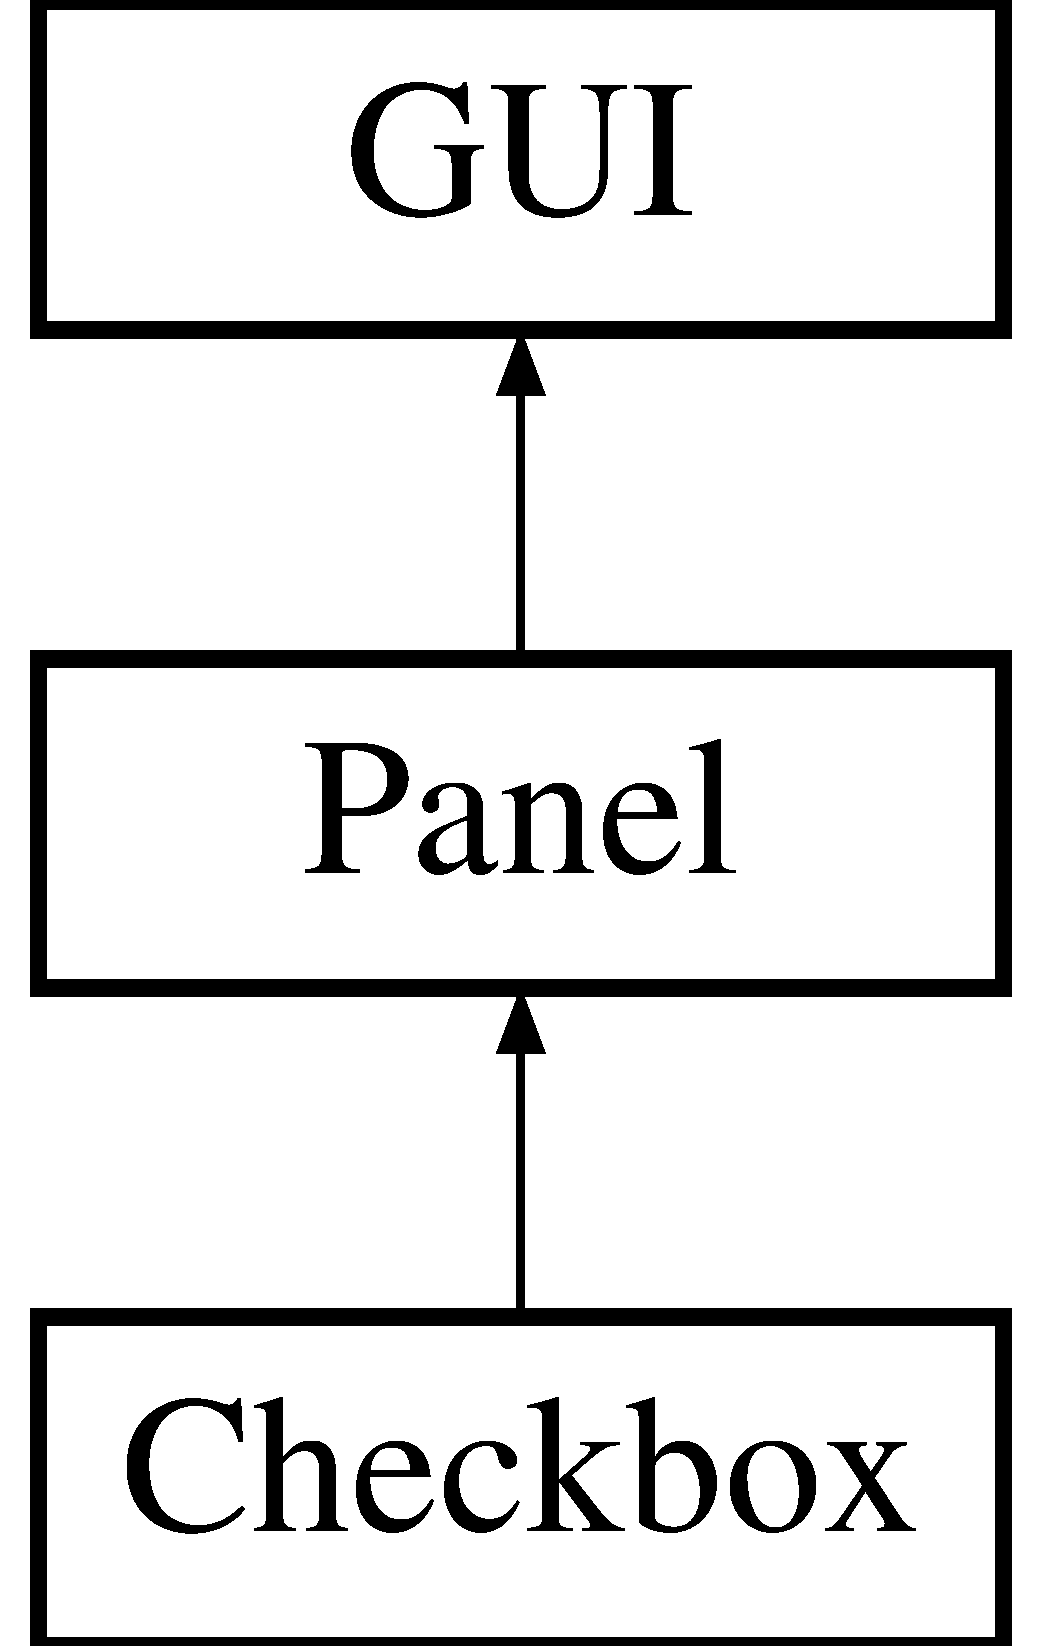
\includegraphics[height=3.000000cm]{class_checkbox}
\end{center}
\end{figure}
\subsection*{Public Member Functions}
\begin{DoxyCompactItemize}
\item 
\mbox{\hyperlink{class_checkbox_aef583c2ed2cc9004aec3330f9b9d02a3}{Checkbox}} (float \mbox{\hyperlink{class_g_u_i_a7fa193a8ffb27bbb3bcc225e36f6d54d}{x}}, float \mbox{\hyperlink{class_g_u_i_a98f204f99ffc5ff6cffc9340bbb8c29b}{y}}, float \mbox{\hyperlink{class_g_u_i_aee5d8766834f6f743f0d8b8c16e47155}{width}}, float \mbox{\hyperlink{class_g_u_i_a70b578c36323a45cac88ccff3bced933}{height}}, \mbox{\hyperlink{class_vector4}{Vector4F}} \mbox{\hyperlink{class_checkbox_adf8806f2b48dfe1d415d108f3ef5bc8c}{colour\+\_\+on}}, \mbox{\hyperlink{class_vector4}{Vector4F}} \mbox{\hyperlink{class_checkbox_a09f7af816849a1b505af2e746847fcc4}{colour\+\_\+off}}, \mbox{\hyperlink{class_shader}{Shader}} \&\mbox{\hyperlink{class_g_u_i_a64b007b31d0ec8a8704f9ab3bb2a7d3d}{shader}}, \mbox{\hyperlink{class_mouse_listener}{Mouse\+Listener}} \&\mbox{\hyperlink{class_checkbox_a7cf00bf1e5b41dcf590e7e836e937ead}{mouse\+\_\+listener}}, bool ticked=false)
\item 
virtual void \mbox{\hyperlink{class_checkbox_a69c9fb9ce334fc8ff76c49447f1e002d}{update}} () override
\item 
virtual bool \mbox{\hyperlink{class_checkbox_a2a2c82a9e8c95ad868ce85a60ba07292}{focused}} () const override
\item 
virtual bool \mbox{\hyperlink{class_checkbox_a63fc27bae94d81d4dee8cd2d0e474d2b}{is\+\_\+mouse\+\_\+sensitive}} () const override
\item 
bool \mbox{\hyperlink{class_checkbox_a6780c6fb30c8b7cec8b55943ec31f1f4}{moused\+\_\+over}} () const
\item 
bool \mbox{\hyperlink{class_checkbox_a67e81d283ae9ead851c902572096bd99}{clicked\+\_\+on}} () const
\item 
const \mbox{\hyperlink{class_vector4}{Vector4F}} \& \mbox{\hyperlink{class_checkbox_accb44cc4cde3fe6ad7a88b27831fa37a}{get\+\_\+colour\+\_\+on}} () const
\item 
const \mbox{\hyperlink{class_vector4}{Vector4F}} \& \mbox{\hyperlink{class_checkbox_ac99d837db8754756bcaa417e96162844}{get\+\_\+colour\+\_\+off}} () const
\item 
\mbox{\hyperlink{class_vector4}{Vector4F}} \mbox{\hyperlink{class_checkbox_ada05d14b0502bc3534c83478b7bad8fb}{get\+\_\+colour}} () const
\end{DoxyCompactItemize}
\subsection*{Public Attributes}
\begin{DoxyCompactItemize}
\item 
\mbox{\Hypertarget{class_checkbox_ac423af3bf4b58bc68ce79392ce11b291}\label{class_checkbox_ac423af3bf4b58bc68ce79392ce11b291}} 
bool \mbox{\hyperlink{class_checkbox_ac423af3bf4b58bc68ce79392ce11b291}{value}}
\begin{DoxyCompactList}\small\item\em Stores whether the \mbox{\hyperlink{class_checkbox}{Checkbox}} is checked or not. \end{DoxyCompactList}\end{DoxyCompactItemize}
\subsection*{Protected Member Functions}
\begin{DoxyCompactItemize}
\item 
bool \mbox{\hyperlink{class_checkbox_a7d468fd5e0d9be7eeb498f511fa23f16}{is\+\_\+choice}} () const
\end{DoxyCompactItemize}
\subsection*{Protected Attributes}
\begin{DoxyCompactItemize}
\item 
\mbox{\Hypertarget{class_checkbox_adf8806f2b48dfe1d415d108f3ef5bc8c}\label{class_checkbox_adf8806f2b48dfe1d415d108f3ef5bc8c}} 
\mbox{\hyperlink{class_vector4}{Vector4F}} \mbox{\hyperlink{class_checkbox_adf8806f2b48dfe1d415d108f3ef5bc8c}{colour\+\_\+on}}
\begin{DoxyCompactList}\small\item\em The colour of the \mbox{\hyperlink{class_checkbox}{Checkbox}} foreground when the box is checked. \end{DoxyCompactList}\item 
\mbox{\Hypertarget{class_checkbox_a09f7af816849a1b505af2e746847fcc4}\label{class_checkbox_a09f7af816849a1b505af2e746847fcc4}} 
\mbox{\hyperlink{class_vector4}{Vector4F}} \mbox{\hyperlink{class_checkbox_a09f7af816849a1b505af2e746847fcc4}{colour\+\_\+off}}
\begin{DoxyCompactList}\small\item\em The colour of the \mbox{\hyperlink{class_checkbox}{Checkbox}} foreground when the box is unchecked. \end{DoxyCompactList}\item 
\mbox{\Hypertarget{class_checkbox_a7cf00bf1e5b41dcf590e7e836e937ead}\label{class_checkbox_a7cf00bf1e5b41dcf590e7e836e937ead}} 
\mbox{\hyperlink{class_mouse_listener}{Mouse\+Listener}} \& \mbox{\hyperlink{class_checkbox_a7cf00bf1e5b41dcf590e7e836e937ead}{mouse\+\_\+listener}}
\begin{DoxyCompactList}\small\item\em \mbox{\hyperlink{class_mouse_listener}{Mouse\+Listener}} to control mouse events. \end{DoxyCompactList}\item 
\mbox{\Hypertarget{class_checkbox_af3cb6394e0b1d37a504ff4eaca946aa8}\label{class_checkbox_af3cb6394e0b1d37a504ff4eaca946aa8}} 
bool \mbox{\hyperlink{class_checkbox_af3cb6394e0b1d37a504ff4eaca946aa8}{just\+\_\+clicked}}
\begin{DoxyCompactList}\small\item\em Stores whether the \mbox{\hyperlink{class_button}{Button}} was clicked last frame. \end{DoxyCompactList}\item 
\mbox{\Hypertarget{class_checkbox_afbbde2ae6d330fb75a26210642407b1f}\label{class_checkbox_afbbde2ae6d330fb75a26210642407b1f}} 
bool \mbox{\hyperlink{class_checkbox_afbbde2ae6d330fb75a26210642407b1f}{just\+\_\+moused\+\_\+over}}
\begin{DoxyCompactList}\small\item\em Stores whether the \mbox{\hyperlink{class_button}{Button}} was moused-\/over last frame. \end{DoxyCompactList}\item 
\mbox{\hyperlink{class_checkbox_choice}{Checkbox\+Choice}} $\ast$ \mbox{\hyperlink{class_checkbox_adf30cd14778fdae212e6c97ec456a700}{choice\+\_\+parent}}
\end{DoxyCompactItemize}
\subsection*{Friends}
\begin{DoxyCompactItemize}
\item 
\mbox{\Hypertarget{class_checkbox_a4b620fd2be6bc41e03130fc79d3ee6a3}\label{class_checkbox_a4b620fd2be6bc41e03130fc79d3ee6a3}} 
class {\bfseries Checkbox\+Choice}
\end{DoxyCompactItemize}


\subsection{Detailed Description}
Graphical representation of a mutable boolean. Use this to enable user-\/input for toggling booleans. 

\subsection{Constructor \& Destructor Documentation}
\mbox{\Hypertarget{class_checkbox_aef583c2ed2cc9004aec3330f9b9d02a3}\label{class_checkbox_aef583c2ed2cc9004aec3330f9b9d02a3}} 
\index{Checkbox@{Checkbox}!Checkbox@{Checkbox}}
\index{Checkbox@{Checkbox}!Checkbox@{Checkbox}}
\subsubsection{\texorpdfstring{Checkbox()}{Checkbox()}}
{\footnotesize\ttfamily Checkbox\+::\+Checkbox (\begin{DoxyParamCaption}\item[{float}]{x,  }\item[{float}]{y,  }\item[{float}]{width,  }\item[{float}]{height,  }\item[{\mbox{\hyperlink{class_vector4}{Vector4F}}}]{colour\+\_\+on,  }\item[{\mbox{\hyperlink{class_vector4}{Vector4F}}}]{colour\+\_\+off,  }\item[{\mbox{\hyperlink{class_shader}{Shader}} \&}]{shader,  }\item[{\mbox{\hyperlink{class_mouse_listener}{Mouse\+Listener}} \&}]{mouse\+\_\+listener,  }\item[{bool}]{ticked = {\ttfamily false} }\end{DoxyParamCaption})}

Construct a Check\+Box with all specifications. 
\begin{DoxyParams}{Parameters}
{\em x} & -\/ Position of the checkbox on the x-\/axis, in pixels. \\
\hline
{\em y} & -\/ Position of the checkbox on the y-\/axis, in pixels. \\
\hline
{\em width} & -\/ Width of the checkbox, in pixels. \\
\hline
{\em height} & -\/ Height of the checkbox, in pixels. \\
\hline
{\em colour\+\_\+on} & -\/ Colour of the checkbox when it is checked (on). \\
\hline
{\em colour\+\_\+off} & -\/ Colour of the checkbox when it is unchecked (off). \\
\hline
{\em shader} & -\/ The shader with which to render the checkbox. \\
\hline
{\em mouse\+\_\+listener} & -\/ The mouse-\/listener with which to query whether is being clicked or not. \\
\hline
{\em ticked} & -\/ Whether the checkbox should initially be checked or not. \\
\hline
\end{DoxyParams}


\subsection{Member Function Documentation}
\mbox{\Hypertarget{class_checkbox_a67e81d283ae9ead851c902572096bd99}\label{class_checkbox_a67e81d283ae9ead851c902572096bd99}} 
\index{Checkbox@{Checkbox}!clicked\+\_\+on@{clicked\+\_\+on}}
\index{clicked\+\_\+on@{clicked\+\_\+on}!Checkbox@{Checkbox}}
\subsubsection{\texorpdfstring{clicked\+\_\+on()}{clicked\_on()}}
{\footnotesize\ttfamily bool Checkbox\+::clicked\+\_\+on (\begin{DoxyParamCaption}{ }\end{DoxyParamCaption}) const}

Query whether the checkbox is currently being clicked on. \begin{DoxyReturn}{Returns}
-\/ True if the checkbox is being clicked on. False otherwise 
\end{DoxyReturn}
\mbox{\Hypertarget{class_checkbox_a2a2c82a9e8c95ad868ce85a60ba07292}\label{class_checkbox_a2a2c82a9e8c95ad868ce85a60ba07292}} 
\index{Checkbox@{Checkbox}!focused@{focused}}
\index{focused@{focused}!Checkbox@{Checkbox}}
\subsubsection{\texorpdfstring{focused()}{focused()}}
{\footnotesize\ttfamily bool Checkbox\+::focused (\begin{DoxyParamCaption}{ }\end{DoxyParamCaption}) const\hspace{0.3cm}{\ttfamily [override]}, {\ttfamily [virtual]}}

Query whether the checkbox is focused or not. \begin{DoxyReturn}{Returns}
-\/ True if the checkbox is focused. False otherwise 
\end{DoxyReturn}


Reimplemented from \mbox{\hyperlink{class_panel_ace2217419ea5c2e98a38678c6e2012e1}{Panel}}.

\mbox{\Hypertarget{class_checkbox_ada05d14b0502bc3534c83478b7bad8fb}\label{class_checkbox_ada05d14b0502bc3534c83478b7bad8fb}} 
\index{Checkbox@{Checkbox}!get\+\_\+colour@{get\+\_\+colour}}
\index{get\+\_\+colour@{get\+\_\+colour}!Checkbox@{Checkbox}}
\subsubsection{\texorpdfstring{get\+\_\+colour()}{get\_colour()}}
{\footnotesize\ttfamily \mbox{\hyperlink{class_vector4}{Vector4F}} Checkbox\+::get\+\_\+colour (\begin{DoxyParamCaption}{ }\end{DoxyParamCaption}) const}

Get R\+G\+B\+A-\/coded colour of the checkbox. This colour depends on whether it is checked or not. \begin{DoxyReturn}{Returns}
-\/ Current colour of the checkbox. 
\end{DoxyReturn}
\mbox{\Hypertarget{class_checkbox_ac99d837db8754756bcaa417e96162844}\label{class_checkbox_ac99d837db8754756bcaa417e96162844}} 
\index{Checkbox@{Checkbox}!get\+\_\+colour\+\_\+off@{get\+\_\+colour\+\_\+off}}
\index{get\+\_\+colour\+\_\+off@{get\+\_\+colour\+\_\+off}!Checkbox@{Checkbox}}
\subsubsection{\texorpdfstring{get\+\_\+colour\+\_\+off()}{get\_colour\_off()}}
{\footnotesize\ttfamily const \mbox{\hyperlink{class_vector4}{Vector4F}} \& Checkbox\+::get\+\_\+colour\+\_\+off (\begin{DoxyParamCaption}{ }\end{DoxyParamCaption}) const}

Get R\+G\+B\+A-\/coded colour of the checkbox when it is unchecked. \begin{DoxyReturn}{Returns}
-\/ Colour of the checkbox when unchecked. 
\end{DoxyReturn}
\mbox{\Hypertarget{class_checkbox_accb44cc4cde3fe6ad7a88b27831fa37a}\label{class_checkbox_accb44cc4cde3fe6ad7a88b27831fa37a}} 
\index{Checkbox@{Checkbox}!get\+\_\+colour\+\_\+on@{get\+\_\+colour\+\_\+on}}
\index{get\+\_\+colour\+\_\+on@{get\+\_\+colour\+\_\+on}!Checkbox@{Checkbox}}
\subsubsection{\texorpdfstring{get\+\_\+colour\+\_\+on()}{get\_colour\_on()}}
{\footnotesize\ttfamily const \mbox{\hyperlink{class_vector4}{Vector4F}} \& Checkbox\+::get\+\_\+colour\+\_\+on (\begin{DoxyParamCaption}{ }\end{DoxyParamCaption}) const}

Get R\+G\+B\+A-\/coded colour of the checkbox when it is checked. \begin{DoxyReturn}{Returns}
-\/ Colour of the checkbox when checked. 
\end{DoxyReturn}
\mbox{\Hypertarget{class_checkbox_a7d468fd5e0d9be7eeb498f511fa23f16}\label{class_checkbox_a7d468fd5e0d9be7eeb498f511fa23f16}} 
\index{Checkbox@{Checkbox}!is\+\_\+choice@{is\+\_\+choice}}
\index{is\+\_\+choice@{is\+\_\+choice}!Checkbox@{Checkbox}}
\subsubsection{\texorpdfstring{is\+\_\+choice()}{is\_choice()}}
{\footnotesize\ttfamily bool Checkbox\+::is\+\_\+choice (\begin{DoxyParamCaption}{ }\end{DoxyParamCaption}) const\hspace{0.3cm}{\ttfamily [protected]}}

Queries the \mbox{\hyperlink{class_checkbox_choice}{Checkbox\+Choice}} parent whether this is the chosen \mbox{\hyperlink{class_checkbox}{Checkbox}}. \begin{DoxyReturn}{Returns}
-\/ True if there exists a \mbox{\hyperlink{class_checkbox_choice}{Checkbox\+Choice}} parent, and it specifies this \mbox{\hyperlink{class_checkbox}{Checkbox}} as the selected box. False otherwise 
\end{DoxyReturn}
\mbox{\Hypertarget{class_checkbox_a63fc27bae94d81d4dee8cd2d0e474d2b}\label{class_checkbox_a63fc27bae94d81d4dee8cd2d0e474d2b}} 
\index{Checkbox@{Checkbox}!is\+\_\+mouse\+\_\+sensitive@{is\+\_\+mouse\+\_\+sensitive}}
\index{is\+\_\+mouse\+\_\+sensitive@{is\+\_\+mouse\+\_\+sensitive}!Checkbox@{Checkbox}}
\subsubsection{\texorpdfstring{is\+\_\+mouse\+\_\+sensitive()}{is\_mouse\_sensitive()}}
{\footnotesize\ttfamily virtual bool Checkbox\+::is\+\_\+mouse\+\_\+sensitive (\begin{DoxyParamCaption}{ }\end{DoxyParamCaption}) const\hspace{0.3cm}{\ttfamily [inline]}, {\ttfamily [override]}, {\ttfamily [virtual]}}

Checkboxes are always mouse sensitive. \begin{DoxyReturn}{Returns}
-\/ True 
\end{DoxyReturn}


Reimplemented from \mbox{\hyperlink{class_panel_a607fe6e1be6fd056f199fa817a4dedda}{Panel}}.

\mbox{\Hypertarget{class_checkbox_a6780c6fb30c8b7cec8b55943ec31f1f4}\label{class_checkbox_a6780c6fb30c8b7cec8b55943ec31f1f4}} 
\index{Checkbox@{Checkbox}!moused\+\_\+over@{moused\+\_\+over}}
\index{moused\+\_\+over@{moused\+\_\+over}!Checkbox@{Checkbox}}
\subsubsection{\texorpdfstring{moused\+\_\+over()}{moused\_over()}}
{\footnotesize\ttfamily bool Checkbox\+::moused\+\_\+over (\begin{DoxyParamCaption}{ }\end{DoxyParamCaption}) const}

Query whether the checkbox is currently being moused-\/over. \begin{DoxyReturn}{Returns}
-\/ True if the checkbox is moused-\/over. False otherwise 
\end{DoxyReturn}
\mbox{\Hypertarget{class_checkbox_a69c9fb9ce334fc8ff76c49447f1e002d}\label{class_checkbox_a69c9fb9ce334fc8ff76c49447f1e002d}} 
\index{Checkbox@{Checkbox}!update@{update}}
\index{update@{update}!Checkbox@{Checkbox}}
\subsubsection{\texorpdfstring{update()}{update()}}
{\footnotesize\ttfamily void Checkbox\+::update (\begin{DoxyParamCaption}{ }\end{DoxyParamCaption})\hspace{0.3cm}{\ttfamily [override]}, {\ttfamily [virtual]}}

Render and update all children. 

Reimplemented from \mbox{\hyperlink{class_panel_a9e9c0608cf3139833cde6b73dc3ba443}{Panel}}.



\subsection{Member Data Documentation}
\mbox{\Hypertarget{class_checkbox_adf30cd14778fdae212e6c97ec456a700}\label{class_checkbox_adf30cd14778fdae212e6c97ec456a700}} 
\index{Checkbox@{Checkbox}!choice\+\_\+parent@{choice\+\_\+parent}}
\index{choice\+\_\+parent@{choice\+\_\+parent}!Checkbox@{Checkbox}}
\subsubsection{\texorpdfstring{choice\+\_\+parent}{choice\_parent}}
{\footnotesize\ttfamily \mbox{\hyperlink{class_checkbox_choice}{Checkbox\+Choice}}$\ast$ Checkbox\+::choice\+\_\+parent\hspace{0.3cm}{\ttfamily [protected]}}

choice\+\_\+parent is handled purely by the friend-\/class \mbox{\hyperlink{class_checkbox_choice}{Checkbox\+Choice}}. 

The documentation for this class was generated from the following files\+:\begin{DoxyCompactItemize}
\item 
src/graphics/gui\+\_\+widget.\+hpp\item 
src/graphics/gui\+\_\+widget.\+cpp\end{DoxyCompactItemize}

\hypertarget{class_checkbox_choice}{}\section{Checkbox\+Choice Class Reference}
\label{class_checkbox_choice}\index{Checkbox\+Choice@{Checkbox\+Choice}}


{\ttfamily \#include $<$gui\+\_\+widget.\+hpp$>$}

\subsection*{Public Member Functions}
\begin{DoxyCompactItemize}
\item 
\mbox{\hyperlink{class_checkbox_choice_aef739358c920959f7158498af135d261}{Checkbox\+Choice}} (std\+::initializer\+\_\+list$<$ \mbox{\hyperlink{class_checkbox}{Checkbox}} $\ast$$>$ boxes, \mbox{\hyperlink{class_checkbox}{Checkbox}} $\ast$initial\+\_\+choice=nullptr)
\item 
\mbox{\hyperlink{class_checkbox_choice_acbbc8db19fa53fc73c913780e0fb2b89}{Checkbox\+Choice}} (std\+::initializer\+\_\+list$<$ std\+::reference\+\_\+wrapper$<$ \mbox{\hyperlink{class_checkbox}{Checkbox}} $>$$>$ boxes, \mbox{\hyperlink{class_checkbox}{Checkbox}} $\ast$initial\+\_\+choice=nullptr)
\item 
\mbox{\hyperlink{class_checkbox_choice_a1434699c2e3295b5037010403cbab6c9}{Checkbox\+Choice}} (const \mbox{\hyperlink{class_checkbox_choice}{Checkbox\+Choice}} \&copy)=delete
\item 
\mbox{\hyperlink{class_checkbox_choice_a907edd806c8e5a7ef45fdc64c013f4eb}{Checkbox\+Choice}} (\mbox{\hyperlink{class_checkbox_choice}{Checkbox\+Choice}} \&\&move)=default
\item 
\mbox{\hyperlink{class_checkbox_choice}{Checkbox\+Choice}} \& \mbox{\hyperlink{class_checkbox_choice_a8e99359a312be66fed6837c768e9e184}{operator=}} (const \mbox{\hyperlink{class_checkbox_choice}{Checkbox\+Choice}} \&rhs)=delete
\item 
\mbox{\hyperlink{class_checkbox_choice}{Checkbox\+Choice}} \& \mbox{\hyperlink{class_checkbox_choice_a8afcd170a63e030912620c18b0527fe8}{operator=}} (\mbox{\hyperlink{class_checkbox_choice}{Checkbox\+Choice}} \&\&rhs)=default
\item 
\mbox{\Hypertarget{class_checkbox_choice_a6fd60881829607567eac28ba82c6a5b4}\label{class_checkbox_choice_a6fd60881829607567eac28ba82c6a5b4}} 
bool {\bfseries has\+\_\+choice} () const
\item 
\mbox{\Hypertarget{class_checkbox_choice_a61b7eedbf1aa28060ac22b47039b060a}\label{class_checkbox_choice_a61b7eedbf1aa28060ac22b47039b060a}} 
\mbox{\hyperlink{class_checkbox}{Checkbox}} $\ast$ {\bfseries get\+\_\+choice} () const
\item 
\mbox{\Hypertarget{class_checkbox_choice_a02298a96989fb9c74de92e3094a51466}\label{class_checkbox_choice_a02298a96989fb9c74de92e3094a51466}} 
void {\bfseries set\+\_\+choice} (\mbox{\hyperlink{class_checkbox}{Checkbox}} $\ast$choice)
\item 
\mbox{\Hypertarget{class_checkbox_choice_a76ea2985a33d1b48b637d049f55c2443}\label{class_checkbox_choice_a76ea2985a33d1b48b637d049f55c2443}} 
const std\+::unordered\+\_\+set$<$ \mbox{\hyperlink{class_checkbox}{Checkbox}} $\ast$ $>$ \& {\bfseries get\+\_\+bool\+\_\+boxes} () const
\end{DoxyCompactItemize}


\subsection{Detailed Description}
Non-\/owning helper class to manage multiple Checkboxes. Use this to allow multiple checkboxes to only have one truthy at a time. 

\subsection{Constructor \& Destructor Documentation}
\mbox{\Hypertarget{class_checkbox_choice_aef739358c920959f7158498af135d261}\label{class_checkbox_choice_aef739358c920959f7158498af135d261}} 
\index{Checkbox\+Choice@{Checkbox\+Choice}!Checkbox\+Choice@{Checkbox\+Choice}}
\index{Checkbox\+Choice@{Checkbox\+Choice}!Checkbox\+Choice@{Checkbox\+Choice}}
\subsubsection{\texorpdfstring{Checkbox\+Choice()}{CheckboxChoice()}\hspace{0.1cm}{\footnotesize\ttfamily [1/4]}}
{\footnotesize\ttfamily Checkbox\+Choice\+::\+Checkbox\+Choice (\begin{DoxyParamCaption}\item[{std\+::initializer\+\_\+list$<$ \mbox{\hyperlink{class_checkbox}{Checkbox}} $\ast$$>$}]{boxes,  }\item[{\mbox{\hyperlink{class_checkbox}{Checkbox}} $\ast$}]{initial\+\_\+choice = {\ttfamily nullptr} }\end{DoxyParamCaption})}

Non-\/owning pointer initialisation. \mbox{\Hypertarget{class_checkbox_choice_acbbc8db19fa53fc73c913780e0fb2b89}\label{class_checkbox_choice_acbbc8db19fa53fc73c913780e0fb2b89}} 
\index{Checkbox\+Choice@{Checkbox\+Choice}!Checkbox\+Choice@{Checkbox\+Choice}}
\index{Checkbox\+Choice@{Checkbox\+Choice}!Checkbox\+Choice@{Checkbox\+Choice}}
\subsubsection{\texorpdfstring{Checkbox\+Choice()}{CheckboxChoice()}\hspace{0.1cm}{\footnotesize\ttfamily [2/4]}}
{\footnotesize\ttfamily Checkbox\+Choice\+::\+Checkbox\+Choice (\begin{DoxyParamCaption}\item[{std\+::initializer\+\_\+list$<$ std\+::reference\+\_\+wrapper$<$ \mbox{\hyperlink{class_checkbox}{Checkbox}} $>$$>$}]{boxes,  }\item[{\mbox{\hyperlink{class_checkbox}{Checkbox}} $\ast$}]{initial\+\_\+choice = {\ttfamily nullptr} }\end{DoxyParamCaption})}

Non-\/owning reference initialisation. \mbox{\Hypertarget{class_checkbox_choice_a1434699c2e3295b5037010403cbab6c9}\label{class_checkbox_choice_a1434699c2e3295b5037010403cbab6c9}} 
\index{Checkbox\+Choice@{Checkbox\+Choice}!Checkbox\+Choice@{Checkbox\+Choice}}
\index{Checkbox\+Choice@{Checkbox\+Choice}!Checkbox\+Choice@{Checkbox\+Choice}}
\subsubsection{\texorpdfstring{Checkbox\+Choice()}{CheckboxChoice()}\hspace{0.1cm}{\footnotesize\ttfamily [3/4]}}
{\footnotesize\ttfamily Checkbox\+Choice\+::\+Checkbox\+Choice (\begin{DoxyParamCaption}\item[{const \mbox{\hyperlink{class_checkbox_choice}{Checkbox\+Choice}} \&}]{copy }\end{DoxyParamCaption})\hspace{0.3cm}{\ttfamily [delete]}}

Copy constructor deleted. This is because any two Checkbox\+Choices may not share a single element, or \char`\"{}choice-\/fighting\char`\"{} will occur. Choice-\/fighting is the phenomenon such that multiple Checkbox\+Choices choose different boxes to truthify, causing the latter to always invalidate the former. \mbox{\Hypertarget{class_checkbox_choice_a907edd806c8e5a7ef45fdc64c013f4eb}\label{class_checkbox_choice_a907edd806c8e5a7ef45fdc64c013f4eb}} 
\index{Checkbox\+Choice@{Checkbox\+Choice}!Checkbox\+Choice@{Checkbox\+Choice}}
\index{Checkbox\+Choice@{Checkbox\+Choice}!Checkbox\+Choice@{Checkbox\+Choice}}
\subsubsection{\texorpdfstring{Checkbox\+Choice()}{CheckboxChoice()}\hspace{0.1cm}{\footnotesize\ttfamily [4/4]}}
{\footnotesize\ttfamily Checkbox\+Choice\+::\+Checkbox\+Choice (\begin{DoxyParamCaption}\item[{\mbox{\hyperlink{class_checkbox_choice}{Checkbox\+Choice}} \&\&}]{move }\end{DoxyParamCaption})\hspace{0.3cm}{\ttfamily [default]}}

Move constructor implies the rvalue-\/reference parameter is about to go out-\/of-\/scope, meaning that it will not be available to cause choice-\/fighting. For this reason, the move constructor is available. 

\subsection{Member Function Documentation}
\mbox{\Hypertarget{class_checkbox_choice_a8e99359a312be66fed6837c768e9e184}\label{class_checkbox_choice_a8e99359a312be66fed6837c768e9e184}} 
\index{Checkbox\+Choice@{Checkbox\+Choice}!operator=@{operator=}}
\index{operator=@{operator=}!Checkbox\+Choice@{Checkbox\+Choice}}
\subsubsection{\texorpdfstring{operator=()}{operator=()}\hspace{0.1cm}{\footnotesize\ttfamily [1/2]}}
{\footnotesize\ttfamily \mbox{\hyperlink{class_checkbox_choice}{Checkbox\+Choice}}\& Checkbox\+Choice\+::operator= (\begin{DoxyParamCaption}\item[{const \mbox{\hyperlink{class_checkbox_choice}{Checkbox\+Choice}} \&}]{rhs }\end{DoxyParamCaption})\hspace{0.3cm}{\ttfamily [delete]}}

Copy assignment operator is also deleted for the same reason; choice-\/fighting. \mbox{\Hypertarget{class_checkbox_choice_a8afcd170a63e030912620c18b0527fe8}\label{class_checkbox_choice_a8afcd170a63e030912620c18b0527fe8}} 
\index{Checkbox\+Choice@{Checkbox\+Choice}!operator=@{operator=}}
\index{operator=@{operator=}!Checkbox\+Choice@{Checkbox\+Choice}}
\subsubsection{\texorpdfstring{operator=()}{operator=()}\hspace{0.1cm}{\footnotesize\ttfamily [2/2]}}
{\footnotesize\ttfamily \mbox{\hyperlink{class_checkbox_choice}{Checkbox\+Choice}}\& Checkbox\+Choice\+::operator= (\begin{DoxyParamCaption}\item[{\mbox{\hyperlink{class_checkbox_choice}{Checkbox\+Choice}} \&\&}]{rhs }\end{DoxyParamCaption})\hspace{0.3cm}{\ttfamily [default]}}

Similarly to the move constructor, the move assignment-\/operator cannot induce choice-\/fighting so remains available for use. 

The documentation for this class was generated from the following files\+:\begin{DoxyCompactItemize}
\item 
src/graphics/gui\+\_\+widget.\+hpp\item 
src/graphics/gui\+\_\+widget.\+cpp\end{DoxyCompactItemize}

\hypertarget{class_command}{}\section{Command Class Reference}
\label{class_command}\index{Command@{Command}}


{\ttfamily \#include $<$command.\+hpp$>$}

Inheritance diagram for Command\+:\begin{figure}[H]
\begin{center}
\leavevmode
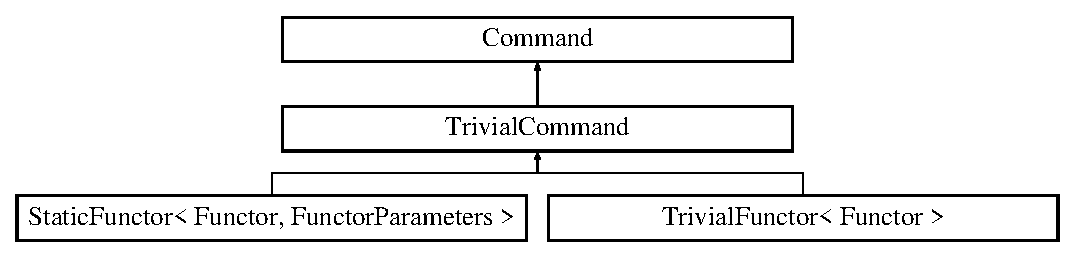
\includegraphics[height=3.000000cm]{class_command}
\end{center}
\end{figure}
\subsection*{Public Member Functions}
\begin{DoxyCompactItemize}
\item 
\mbox{\Hypertarget{class_command_a3cf1e15c821380f4a12e8bd9da620da9}\label{class_command_a3cf1e15c821380f4a12e8bd9da620da9}} 
{\bfseries Command} (std\+::string name=\char`\"{}\char`\"{}, std\+::string description=\char`\"{}\char`\"{}, std\+::string usage=\char`\"{}\char`\"{}, bool trivial=true)
\item 
\mbox{\Hypertarget{class_command_a3d073078862b0cae3b4402f1e4c3b66e}\label{class_command_a3d073078862b0cae3b4402f1e4c3b66e}} 
{\bfseries Command} (const \mbox{\hyperlink{class_command}{Command}} \&copy)=default
\item 
\mbox{\Hypertarget{class_command_a4d99c9b56882eb7f9294ac9ba8e986f2}\label{class_command_a4d99c9b56882eb7f9294ac9ba8e986f2}} 
{\bfseries Command} (\mbox{\hyperlink{class_command}{Command}} \&\&move)=default
\item 
\mbox{\Hypertarget{class_command_ac482b3ec7da68a7173173e41410b3858}\label{class_command_ac482b3ec7da68a7173173e41410b3858}} 
\mbox{\hyperlink{class_command}{Command}} \& {\bfseries operator=} (const \mbox{\hyperlink{class_command}{Command}} \&rhs)=default
\item 
\mbox{\Hypertarget{class_command_afc03c74d1f90127326015faa8f5f4866}\label{class_command_afc03c74d1f90127326015faa8f5f4866}} 
const std\+::string \& {\bfseries get\+\_\+name} () const
\item 
\mbox{\Hypertarget{class_command_a6352942f26bc7f233584ee707ac46eb1}\label{class_command_a6352942f26bc7f233584ee707ac46eb1}} 
const std\+::string \& {\bfseries get\+\_\+description} () const
\item 
\mbox{\Hypertarget{class_command_a0a07c4f1b9b78074268653129bbd6cbb}\label{class_command_a0a07c4f1b9b78074268653129bbd6cbb}} 
const std\+::string \& {\bfseries get\+\_\+usage} () const
\item 
\mbox{\Hypertarget{class_command_ae1e1b915dfc4bbb2633c1b5e331f83e1}\label{class_command_ae1e1b915dfc4bbb2633c1b5e331f83e1}} 
std\+::size\+\_\+t {\bfseries get\+\_\+expected\+\_\+parameter\+\_\+size} () const
\item 
\mbox{\Hypertarget{class_command_a264fd55e96d28e7687a42108539bd9cf}\label{class_command_a264fd55e96d28e7687a42108539bd9cf}} 
virtual bool {\bfseries operator==} (const \mbox{\hyperlink{class_command}{Command}} \&rhs) const
\item 
\mbox{\Hypertarget{class_command_a325860d97ad7b70553e3097321ee9952}\label{class_command_a325860d97ad7b70553e3097321ee9952}} 
virtual void {\bfseries operator()} (const std\+::vector$<$ std\+::string $>$ \&args)=0
\item 
\mbox{\Hypertarget{class_command_a2b9c29afe3b2fd50ef1c8664eec56aec}\label{class_command_a2b9c29afe3b2fd50ef1c8664eec56aec}} 
bool {\bfseries is\+\_\+trivial} () const
\end{DoxyCompactItemize}
\subsection*{Protected Attributes}
\begin{DoxyCompactItemize}
\item 
\mbox{\Hypertarget{class_command_ad6a6005f8236039804a33e9b85dcb7b3}\label{class_command_ad6a6005f8236039804a33e9b85dcb7b3}} 
bool {\bfseries trivial}
\end{DoxyCompactItemize}


\subsection{Detailed Description}
Abstract. Not available for non-\/polymorphic use. Represents a hard-\/coded functor with string arguments. Inherit from this to create custom commands (Essential for adding functionality to \mbox{\hyperlink{class_engine}{Engine}}). For simpler functions with no parameters, use a \mbox{\hyperlink{class_trivial_command}{Trivial\+Command}} instead (see lower down this source file). 

The documentation for this class was generated from the following files\+:\begin{DoxyCompactItemize}
\item 
src/command.\+hpp\item 
src/command.\+cpp\end{DoxyCompactItemize}

\hypertarget{class_command_executor}{}\section{Command\+Executor Class Reference}
\label{class_command_executor}\index{Command\+Executor@{Command\+Executor}}


{\ttfamily \#include $<$command.\+hpp$>$}

\subsection*{Public Member Functions}
\begin{DoxyCompactItemize}
\item 
\mbox{\Hypertarget{class_command_executor_a79b6bc00111839e0eb3ca4f25078f4df}\label{class_command_executor_a79b6bc00111839e0eb3ca4f25078f4df}} 
{\bfseries Command\+Executor} (const \mbox{\hyperlink{class_command_executor}{Command\+Executor}} \&copy)=default
\item 
\mbox{\Hypertarget{class_command_executor_a3441b23c3b3061f0906d5fa837c15c18}\label{class_command_executor_a3441b23c3b3061f0906d5fa837c15c18}} 
{\bfseries Command\+Executor} (\mbox{\hyperlink{class_command_executor}{Command\+Executor}} \&\&move)=default
\item 
\mbox{\Hypertarget{class_command_executor_a3cb5c70e729192b34b96b5fcbf65acf0}\label{class_command_executor_a3cb5c70e729192b34b96b5fcbf65acf0}} 
\mbox{\hyperlink{class_command_executor}{Command\+Executor}} \& {\bfseries operator=} (const \mbox{\hyperlink{class_command_executor}{Command\+Executor}} \&rhs)=default
\item 
\mbox{\Hypertarget{class_command_executor_a60a3ab2b3f7fde5c64bd213461061126}\label{class_command_executor_a60a3ab2b3f7fde5c64bd213461061126}} 
std\+::unordered\+\_\+set$<$ \mbox{\hyperlink{class_command}{Command}} $\ast$ $>$ {\bfseries get\+\_\+commands} () const
\item 
\mbox{\Hypertarget{class_command_executor_a37052aaf61623b511be1f75cbecab8b7}\label{class_command_executor_a37052aaf61623b511be1f75cbecab8b7}} 
void {\bfseries register\+\_\+command} (\mbox{\hyperlink{class_command}{Command}} $\ast$command)
\item 
\mbox{\Hypertarget{class_command_executor_a988168a9e22cc38d309dd4c7c79921c1}\label{class_command_executor_a988168a9e22cc38d309dd4c7c79921c1}} 
{\footnotesize template$<$typename Functor $>$ }\\\mbox{\hyperlink{class_trivial_functor}{Trivial\+Functor}}$<$ \mbox{\hyperlink{class_functor}{Functor}} $>$ $\ast$ {\bfseries emplace\+\_\+trivial\+\_\+command} (\mbox{\hyperlink{class_functor}{Functor}} \&\&functor)
\item 
\mbox{\Hypertarget{class_command_executor_a745e9fc9e15db7102e50b3b23370fc3d}\label{class_command_executor_a745e9fc9e15db7102e50b3b23370fc3d}} 
{\footnotesize template$<$typename Functor , typename... Functor\+Parameters$>$ }\\\mbox{\hyperlink{class_static_functor}{Static\+Functor}}$<$ \mbox{\hyperlink{class_functor}{Functor}}, Functor\+Parameters... $>$ $\ast$ {\bfseries emplace\+\_\+static\+\_\+command} (\mbox{\hyperlink{class_functor}{Functor}} \&\&functor, Functor\+Parameters \&\&... parameters)
\item 
\mbox{\Hypertarget{class_command_executor_a6f99990af551c26ced617d0c58720c74}\label{class_command_executor_a6f99990af551c26ced617d0c58720c74}} 
void {\bfseries deregister\+\_\+command} (\mbox{\hyperlink{class_command}{Command}} $\ast$command)
\item 
\mbox{\Hypertarget{class_command_executor_ae4af9df5bdf49a97f3efaf483f53c97b}\label{class_command_executor_ae4af9df5bdf49a97f3efaf483f53c97b}} 
void {\bfseries deregister\+\_\+command} (const std\+::string \&command\+\_\+name)
\item 
\mbox{\Hypertarget{class_command_executor_a1076730c7e82e790ed11566677883b5e}\label{class_command_executor_a1076730c7e82e790ed11566677883b5e}} 
void {\bfseries operator()} (const std\+::string \&name, const std\+::vector$<$ std\+::string $>$ \&args=std\+::vector$<$ std\+::string $>$())
\end{DoxyCompactItemize}


\subsection{Detailed Description}
System used to hold (but not typically own) Commands. \mbox{\hyperlink{class_engine}{Engine}} uses these to handle command input. 

The documentation for this class was generated from the following files\+:\begin{DoxyCompactItemize}
\item 
src/command.\+hpp\item 
src/command.\+cpp\item 
src/command.\+inl\end{DoxyCompactItemize}

\hypertarget{class_cube_map}{}\section{Cube\+Map Class Reference}
\label{class_cube_map}\index{Cube\+Map@{Cube\+Map}}


{\ttfamily \#include $<$texture.\+hpp$>$}

\subsection*{Public Member Functions}
\begin{DoxyCompactItemize}
\item 
\mbox{\Hypertarget{class_cube_map_a2894dc1765bf0a0534b84b6ac00320c9}\label{class_cube_map_a2894dc1765bf0a0534b84b6ac00320c9}} 
{\bfseries Cube\+Map} (std\+::string right\+\_\+texture, std\+::string left\+\_\+texture, std\+::string top\+\_\+texture, std\+::string bottom\+\_\+texture, std\+::string back\+\_\+texture, std\+::string front\+\_\+texture)
\item 
\mbox{\Hypertarget{class_cube_map_a0d383d15339d920042a6b7c4209f8ab6}\label{class_cube_map_a0d383d15339d920042a6b7c4209f8ab6}} 
{\bfseries Cube\+Map} (std\+::string texture\+\_\+directory=\char`\"{}./\char`\"{}, std\+::string skybox\+\_\+name=\char`\"{}skybox\char`\"{}, std\+::string skybox\+\_\+image\+\_\+file\+\_\+extension=\char`\"{}.png\char`\"{})
\item 
\mbox{\Hypertarget{class_cube_map_a687da9c791db37544c3aab73210b1135}\label{class_cube_map_a687da9c791db37544c3aab73210b1135}} 
{\bfseries Cube\+Map} (const \mbox{\hyperlink{class_cube_map}{Cube\+Map}} \&copy)
\item 
\mbox{\Hypertarget{class_cube_map_a72a09700337e9eabfb3f88bb0bae768e}\label{class_cube_map_a72a09700337e9eabfb3f88bb0bae768e}} 
{\bfseries Cube\+Map} (\mbox{\hyperlink{class_cube_map}{Cube\+Map}} \&\&move)
\item 
\mbox{\Hypertarget{class_cube_map_a847365d5a2e986c553d46bece2a004ad}\label{class_cube_map_a847365d5a2e986c553d46bece2a004ad}} 
\mbox{\hyperlink{class_cube_map}{Cube\+Map}} \& {\bfseries operator=} (const \mbox{\hyperlink{class_cube_map}{Cube\+Map}} \&rhs)=delete
\item 
\mbox{\Hypertarget{class_cube_map_a5d022a37c170ed6f7acb2354a6cae45d}\label{class_cube_map_a5d022a37c170ed6f7acb2354a6cae45d}} 
void {\bfseries bind} (\mbox{\hyperlink{class_shader}{Shader}} $\ast$shader, unsigned int id) const
\end{DoxyCompactItemize}


\subsection{Detailed Description}
Used to construct skyboxes. Requires six textures; for each face of the skybox cube mesh. 

The documentation for this class was generated from the following files\+:\begin{DoxyCompactItemize}
\item 
src/graphics/texture.\+hpp\item 
src/graphics/texture.\+cpp\end{DoxyCompactItemize}

\hypertarget{class_displacement_map}{}\section{Displacement\+Map Class Reference}
\label{class_displacement_map}\index{Displacement\+Map@{Displacement\+Map}}
Inheritance diagram for Displacement\+Map\+:\begin{figure}[H]
\begin{center}
\leavevmode
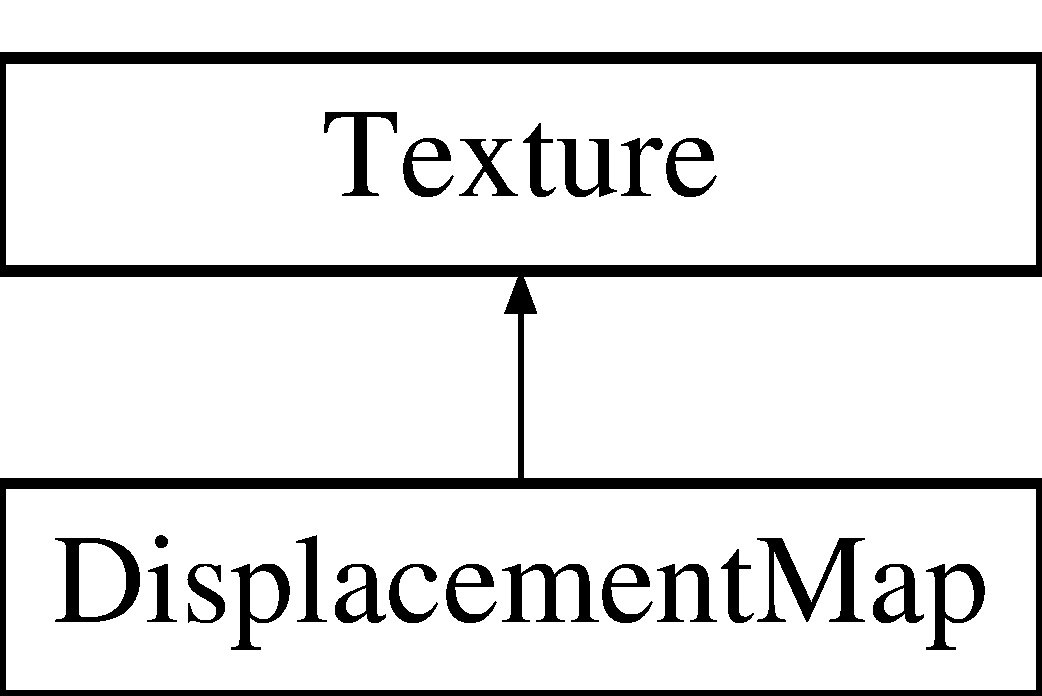
\includegraphics[height=2.000000cm]{class_displacement_map}
\end{center}
\end{figure}
\subsection*{Public Member Functions}
\begin{DoxyCompactItemize}
\item 
\mbox{\Hypertarget{class_displacement_map_ad9fb0c5ac51d5dede9d6cbd0721add36}\label{class_displacement_map_ad9fb0c5ac51d5dede9d6cbd0721add36}} 
{\bfseries Displacement\+Map} (std\+::string filename)
\item 
\mbox{\Hypertarget{class_displacement_map_afbc019ec3ec956d0eac44442d4346274}\label{class_displacement_map_afbc019ec3ec956d0eac44442d4346274}} 
virtual void {\bfseries bind} (\mbox{\hyperlink{class_shader}{Shader}} $\ast$shader, unsigned int id) const override
\item 
\mbox{\Hypertarget{class_displacement_map_a86b4259eb46e198c6d535461c0665019}\label{class_displacement_map_a86b4259eb46e198c6d535461c0665019}} 
virtual tz\+::graphics\+::\+Texture\+Type {\bfseries get\+\_\+texture\+\_\+type} () const override
\end{DoxyCompactItemize}
\subsection*{Additional Inherited Members}


The documentation for this class was generated from the following file\+:\begin{DoxyCompactItemize}
\item 
src/graphics/texture.\+hpp\end{DoxyCompactItemize}

\hypertarget{class_engine}{}\section{Engine Class Reference}
\label{class_engine}\index{Engine@{Engine}}


{\ttfamily \#include $<$engine.\+hpp$>$}

\subsection*{Public Member Functions}
\begin{DoxyCompactItemize}
\item 
\mbox{\hyperlink{class_engine_a1e76f3786243e116f071e98724fe4a25}{Engine}} (\mbox{\hyperlink{class_window}{Window}} $\ast$window, std\+::string properties\+\_\+path=tz\+::default\+\_\+properties\+\_\+path, unsigned int tps=30)
\item 
\mbox{\Hypertarget{class_engine_ae115127e3dcb6916f44b070cd94eec86}\label{class_engine_ae115127e3dcb6916f44b070cd94eec86}} 
{\bfseries Engine} (const \mbox{\hyperlink{class_engine}{Engine}} \&copy)=default
\item 
\mbox{\Hypertarget{class_engine_a21831fd3d22bba5db978ed8f6a5a13e1}\label{class_engine_a21831fd3d22bba5db978ed8f6a5a13e1}} 
{\bfseries Engine} (\mbox{\hyperlink{class_engine}{Engine}} \&\&move)=default
\item 
\mbox{\Hypertarget{class_engine_ab1e81e6840409144537a1ba54d1ad5eb}\label{class_engine_ab1e81e6840409144537a1ba54d1ad5eb}} 
\mbox{\hyperlink{class_engine}{Engine}} \& {\bfseries operator=} (const \mbox{\hyperlink{class_engine}{Engine}} \&rhs)=default
\item 
void \mbox{\hyperlink{class_engine_a12375001d456a8beb1b51c5f97ad6c22}{update}} (std\+::size\+\_\+t shader\+\_\+index=0)
\item 
\mbox{\Hypertarget{class_engine_abaf7e650f53c4d2564de41a9057436c8}\label{class_engine_abaf7e650f53c4d2564de41a9057436c8}} 
const \mbox{\hyperlink{class_time_profiler}{Time\+Profiler}} \& {\bfseries get\+\_\+time\+\_\+profiler} () const
\item 
\mbox{\Hypertarget{class_engine_a54d43658e5b3e49cb0a1f9a1fda4c992}\label{class_engine_a54d43658e5b3e49cb0a1f9a1fda4c992}} 
const \mbox{\hyperlink{class_engine_meta}{Engine\+Meta}} \& {\bfseries get\+\_\+meta} () const
\item 
const \mbox{\hyperlink{class_window}{Window}} \& \mbox{\hyperlink{class_engine_a30c10f14f67c8f6b0b6d0f47393ea31c}{get\+\_\+window}} () const
\item 
const std\+::vector$<$ std\+::unique\+\_\+ptr$<$ \mbox{\hyperlink{class_mesh}{Mesh}} $>$ $>$ \& \mbox{\hyperlink{class_engine_a0cab1935798c43bd3a9f5ed3a4de1f04}{get\+\_\+meshes}} () const
\item 
\mbox{\Hypertarget{class_engine_aba2ff0632dc6d5b5e6a798b7154d3b13}\label{class_engine_aba2ff0632dc6d5b5e6a798b7154d3b13}} 
const std\+::vector$<$ std\+::unique\+\_\+ptr$<$ \mbox{\hyperlink{class_texture}{Texture}} $>$ $>$ \& {\bfseries get\+\_\+textures} () const
\item 
\mbox{\Hypertarget{class_engine_ae5e2a4ccea1d11ed4d6b42066130cda5}\label{class_engine_ae5e2a4ccea1d11ed4d6b42066130cda5}} 
const std\+::vector$<$ std\+::unique\+\_\+ptr$<$ \mbox{\hyperlink{class_normal_map}{Normal\+Map}} $>$ $>$ \& {\bfseries get\+\_\+normal\+\_\+maps} () const
\item 
\mbox{\Hypertarget{class_engine_a58f16cc74f45b8511ad7420169bd7e2f}\label{class_engine_a58f16cc74f45b8511ad7420169bd7e2f}} 
const std\+::vector$<$ std\+::unique\+\_\+ptr$<$ \mbox{\hyperlink{class_parallax_map}{Parallax\+Map}} $>$ $>$ \& {\bfseries get\+\_\+parallax\+\_\+maps} () const
\item 
\mbox{\Hypertarget{class_engine_a7518ed8e410e6cc01ed05c116c146dd5}\label{class_engine_a7518ed8e410e6cc01ed05c116c146dd5}} 
const std\+::vector$<$ std\+::unique\+\_\+ptr$<$ \mbox{\hyperlink{class_displacement_map}{Displacement\+Map}} $>$ $>$ \& {\bfseries get\+\_\+displacement\+\_\+maps} () const
\item 
\mbox{\hyperlink{class_shader}{Shader}} \& \mbox{\hyperlink{class_engine_af92650e3ce3cabf7e527c92ae4917702}{get\+\_\+shader}} (std\+::size\+\_\+t index)
\item 
unsigned int \mbox{\hyperlink{class_engine_a9b33dc683a75b1a3deb14a7280003b38}{get\+\_\+fps}} () const
\item 
unsigned int \mbox{\hyperlink{class_engine_afac8cc0ad1a0c97024dc61683588f22c}{get\+\_\+tps}} () const
\item 
const \mbox{\hyperlink{class_command_executor}{Command\+Executor}} \& \mbox{\hyperlink{class_engine_ab53fa08b25bde47cf3fd63956669fc72}{get\+\_\+update\+\_\+command\+\_\+executor}} () const
\item 
const \mbox{\hyperlink{class_command_executor}{Command\+Executor}} \& \mbox{\hyperlink{class_engine_a457c2c3adbc7baa8b2903b139882fc79}{get\+\_\+tick\+\_\+command\+\_\+executor}} () const
\item 
void \mbox{\hyperlink{class_engine_a50fc8b735ed53d1157316b35959cad00}{add\+\_\+update\+\_\+command}} (\mbox{\hyperlink{class_command}{Command}} $\ast$cmd)
\item 
\mbox{\Hypertarget{class_engine_a999274fb15418af49088371e88687388}\label{class_engine_a999274fb15418af49088371e88687388}} 
{\footnotesize template$<$typename Functor $>$ }\\\mbox{\hyperlink{class_trivial_functor}{Trivial\+Functor}}$<$ \mbox{\hyperlink{class_functor}{Functor}} $>$ $\ast$ {\bfseries emplace\+\_\+trivial\+\_\+update\+\_\+command} (\mbox{\hyperlink{class_functor}{Functor}} \&\&functor)
\item 
\mbox{\Hypertarget{class_engine_a9d9f6b5fa014f2859d3c75fd2ea1f80d}\label{class_engine_a9d9f6b5fa014f2859d3c75fd2ea1f80d}} 
{\footnotesize template$<$typename Functor , typename... Functor\+Parameters$>$ }\\\mbox{\hyperlink{class_static_functor}{Static\+Functor}}$<$ \mbox{\hyperlink{class_functor}{Functor}}, Functor\+Parameters... $>$ $\ast$ {\bfseries emplace\+\_\+static\+\_\+update\+\_\+command} (\mbox{\hyperlink{class_functor}{Functor}} \&\&functor, Functor\+Parameters \&\&... parameters)
\item 
void \mbox{\hyperlink{class_engine_ad02b6f115de1ce69088c5784cc937d04}{remove\+\_\+update\+\_\+command}} (\mbox{\hyperlink{class_command}{Command}} $\ast$cmd)
\item 
void \mbox{\hyperlink{class_engine_ab2355e889851bc53a6a9e151ca2a1e98}{add\+\_\+tick\+\_\+command}} (\mbox{\hyperlink{class_command}{Command}} $\ast$cmd)
\item 
\mbox{\Hypertarget{class_engine_aeaa751493222a6a30e80b18d8d8952c3}\label{class_engine_aeaa751493222a6a30e80b18d8d8952c3}} 
{\footnotesize template$<$typename Functor $>$ }\\\mbox{\hyperlink{class_trivial_functor}{Trivial\+Functor}}$<$ \mbox{\hyperlink{class_functor}{Functor}} $>$ $\ast$ {\bfseries emplace\+\_\+trivial\+\_\+tick\+\_\+command} (\mbox{\hyperlink{class_functor}{Functor}} \&\&functor)
\item 
\mbox{\Hypertarget{class_engine_a003d3f0fc5f1109cc485f8f54d8c5d82}\label{class_engine_a003d3f0fc5f1109cc485f8f54d8c5d82}} 
{\footnotesize template$<$typename Functor , typename... Functor\+Parameters$>$ }\\\mbox{\hyperlink{class_static_functor}{Static\+Functor}}$<$ \mbox{\hyperlink{class_functor}{Functor}}, Functor\+Parameters... $>$ $\ast$ {\bfseries emplace\+\_\+static\+\_\+tick\+\_\+command} (\mbox{\hyperlink{class_functor}{Functor}} \&\&functor, Functor\+Parameters \&\&... parameters)
\item 
void \mbox{\hyperlink{class_engine_abb354476292180d9db9b4b70d3057096}{remove\+\_\+tick\+\_\+command}} (\mbox{\hyperlink{class_command}{Command}} $\ast$cmd)
\item 
bool \mbox{\hyperlink{class_engine_a6ae98509fe0117b583f9edb6812e3363}{is\+\_\+update\+\_\+due}} () const
\end{DoxyCompactItemize}
\subsection*{Public Attributes}
\begin{DoxyCompactItemize}
\item 
\mbox{\hyperlink{class_camera}{Camera}} \mbox{\hyperlink{class_engine_a25924c4045f695c4fb6b6439777b1920}{camera}}
\item 
\mbox{\Hypertarget{class_engine_a24d0973c7d00cf57a07e30f35c87fc64}\label{class_engine_a24d0973c7d00cf57a07e30f35c87fc64}} 
\mbox{\hyperlink{class_scene}{Scene}} {\bfseries scene}
\item 
\mbox{\Hypertarget{class_engine_a1103187e7ed35b93dca517172993f196}\label{class_engine_a1103187e7ed35b93dca517172993f196}} 
\mbox{\hyperlink{class_shader}{Shader}} {\bfseries default\+\_\+shader}
\item 
\mbox{\Hypertarget{class_engine_a3f92dfc32aae2942f2c9409e8ed8438b}\label{class_engine_a3f92dfc32aae2942f2c9409e8ed8438b}} 
\mbox{\hyperlink{class_shader}{Shader}} {\bfseries default\+\_\+gui\+\_\+shader}
\item 
\mbox{\Hypertarget{class_engine_a906df11eaf663141f086919fc4bf88b8}\label{class_engine_a906df11eaf663141f086919fc4bf88b8}} 
const \mbox{\hyperlink{class_texture}{Texture}} {\bfseries default\+\_\+texture}
\item 
\mbox{\Hypertarget{class_engine_ae060d7cef39dc18cf663e839073931ae}\label{class_engine_ae060d7cef39dc18cf663e839073931ae}} 
const \mbox{\hyperlink{class_normal_map}{Normal\+Map}} {\bfseries default\+\_\+normal\+\_\+map}
\item 
\mbox{\Hypertarget{class_engine_a589a3bd13ab32cb0e955b1a7e2c9c49a}\label{class_engine_a589a3bd13ab32cb0e955b1a7e2c9c49a}} 
const \mbox{\hyperlink{class_parallax_map}{Parallax\+Map}} {\bfseries default\+\_\+parallax\+\_\+map}
\item 
\mbox{\Hypertarget{class_engine_a71eb40026060060b3814f3bdca169631}\label{class_engine_a71eb40026060060b3814f3bdca169631}} 
const \mbox{\hyperlink{class_displacement_map}{Displacement\+Map}} {\bfseries default\+\_\+displacement\+\_\+map}
\end{DoxyCompactItemize}


\subsection{Detailed Description}
Hulking class holding pretty much everything you\textquotesingle{}ll need to use Topaz. Due to its verbosity, it is only recommended to use this class for hobbyist/non-\/commercial purposes. Using this essentially provides stabilisers and handholding to using Topaz. 

\subsection{Constructor \& Destructor Documentation}
\mbox{\Hypertarget{class_engine_a1e76f3786243e116f071e98724fe4a25}\label{class_engine_a1e76f3786243e116f071e98724fe4a25}} 
\index{Engine@{Engine}!Engine@{Engine}}
\index{Engine@{Engine}!Engine@{Engine}}
\subsubsection{\texorpdfstring{Engine()}{Engine()}}
{\footnotesize\ttfamily Engine\+::\+Engine (\begin{DoxyParamCaption}\item[{\mbox{\hyperlink{class_window}{Window}} $\ast$}]{window,  }\item[{std\+::string}]{properties\+\_\+path = {\ttfamily tz\+:\+:default\+\_\+properties\+\_\+path},  }\item[{unsigned int}]{tps = {\ttfamily 30} }\end{DoxyParamCaption})}

Constructs the \mbox{\hyperlink{class_engine}{Engine}}. Should be invoked after \mbox{\hyperlink{namespacetz_aeb2530fee0e452e5ba5f4d0d0ebaa797}{tz\+::initialise}} and \mbox{\hyperlink{class_window}{Window}} construction. window = Address of the Topaz window to render into. properties\+\_\+path = The absolute path to the Topaz properties file (normally called properties.\+mdl) tps = Number of tick updates per second (this affects runtime of physics etc, not rendering). Default is 30, although you can use less or more, depending on how precise you need physics etc to run at. 

\subsection{Member Function Documentation}
\mbox{\Hypertarget{class_engine_ab2355e889851bc53a6a9e151ca2a1e98}\label{class_engine_ab2355e889851bc53a6a9e151ca2a1e98}} 
\index{Engine@{Engine}!add\+\_\+tick\+\_\+command@{add\+\_\+tick\+\_\+command}}
\index{add\+\_\+tick\+\_\+command@{add\+\_\+tick\+\_\+command}!Engine@{Engine}}
\subsubsection{\texorpdfstring{add\+\_\+tick\+\_\+command()}{add\_tick\_command()}}
{\footnotesize\ttfamily void Engine\+::add\+\_\+tick\+\_\+command (\begin{DoxyParamCaption}\item[{\mbox{\hyperlink{class_command}{Command}} $\ast$}]{cmd }\end{DoxyParamCaption})}

Add a custom command to the tick command executor. \mbox{\Hypertarget{class_engine_a50fc8b735ed53d1157316b35959cad00}\label{class_engine_a50fc8b735ed53d1157316b35959cad00}} 
\index{Engine@{Engine}!add\+\_\+update\+\_\+command@{add\+\_\+update\+\_\+command}}
\index{add\+\_\+update\+\_\+command@{add\+\_\+update\+\_\+command}!Engine@{Engine}}
\subsubsection{\texorpdfstring{add\+\_\+update\+\_\+command()}{add\_update\_command()}}
{\footnotesize\ttfamily void Engine\+::add\+\_\+update\+\_\+command (\begin{DoxyParamCaption}\item[{\mbox{\hyperlink{class_command}{Command}} $\ast$}]{cmd }\end{DoxyParamCaption})}

Add a custom command to the update comand executor. \mbox{\Hypertarget{class_engine_a9b33dc683a75b1a3deb14a7280003b38}\label{class_engine_a9b33dc683a75b1a3deb14a7280003b38}} 
\index{Engine@{Engine}!get\+\_\+fps@{get\+\_\+fps}}
\index{get\+\_\+fps@{get\+\_\+fps}!Engine@{Engine}}
\subsubsection{\texorpdfstring{get\+\_\+fps()}{get\_fps()}}
{\footnotesize\ttfamily unsigned int Engine\+::get\+\_\+fps (\begin{DoxyParamCaption}{ }\end{DoxyParamCaption}) const}

Get instantaneous fps \mbox{\Hypertarget{class_engine_a0cab1935798c43bd3a9f5ed3a4de1f04}\label{class_engine_a0cab1935798c43bd3a9f5ed3a4de1f04}} 
\index{Engine@{Engine}!get\+\_\+meshes@{get\+\_\+meshes}}
\index{get\+\_\+meshes@{get\+\_\+meshes}!Engine@{Engine}}
\subsubsection{\texorpdfstring{get\+\_\+meshes()}{get\_meshes()}}
{\footnotesize\ttfamily const std\+::vector$<$ std\+::unique\+\_\+ptr$<$ \mbox{\hyperlink{class_mesh}{Mesh}} $>$ $>$ \& Engine\+::get\+\_\+meshes (\begin{DoxyParamCaption}{ }\end{DoxyParamCaption}) const}

Access lists of all assets. \mbox{\Hypertarget{class_engine_af92650e3ce3cabf7e527c92ae4917702}\label{class_engine_af92650e3ce3cabf7e527c92ae4917702}} 
\index{Engine@{Engine}!get\+\_\+shader@{get\+\_\+shader}}
\index{get\+\_\+shader@{get\+\_\+shader}!Engine@{Engine}}
\subsubsection{\texorpdfstring{get\+\_\+shader()}{get\_shader()}}
{\footnotesize\ttfamily \mbox{\hyperlink{class_shader}{Shader}} \& Engine\+::get\+\_\+shader (\begin{DoxyParamCaption}\item[{std\+::size\+\_\+t}]{index }\end{DoxyParamCaption})}

Get shader by index. If index = 0 or is out of range of extra-\/shaders, will return the default shader. Otherwise, it shall return the extra shader at that index. \mbox{\Hypertarget{class_engine_a457c2c3adbc7baa8b2903b139882fc79}\label{class_engine_a457c2c3adbc7baa8b2903b139882fc79}} 
\index{Engine@{Engine}!get\+\_\+tick\+\_\+command\+\_\+executor@{get\+\_\+tick\+\_\+command\+\_\+executor}}
\index{get\+\_\+tick\+\_\+command\+\_\+executor@{get\+\_\+tick\+\_\+command\+\_\+executor}!Engine@{Engine}}
\subsubsection{\texorpdfstring{get\+\_\+tick\+\_\+command\+\_\+executor()}{get\_tick\_command\_executor()}}
{\footnotesize\ttfamily const \mbox{\hyperlink{class_command_executor}{Command\+Executor}} \& Engine\+::get\+\_\+tick\+\_\+command\+\_\+executor (\begin{DoxyParamCaption}{ }\end{DoxyParamCaption}) const}

Read the tick command executor (for physics updates etc) \mbox{\Hypertarget{class_engine_afac8cc0ad1a0c97024dc61683588f22c}\label{class_engine_afac8cc0ad1a0c97024dc61683588f22c}} 
\index{Engine@{Engine}!get\+\_\+tps@{get\+\_\+tps}}
\index{get\+\_\+tps@{get\+\_\+tps}!Engine@{Engine}}
\subsubsection{\texorpdfstring{get\+\_\+tps()}{get\_tps()}}
{\footnotesize\ttfamily unsigned int Engine\+::get\+\_\+tps (\begin{DoxyParamCaption}{ }\end{DoxyParamCaption}) const}

Get the specified number of ticks per second back when the instance was constructed. \mbox{\Hypertarget{class_engine_ab53fa08b25bde47cf3fd63956669fc72}\label{class_engine_ab53fa08b25bde47cf3fd63956669fc72}} 
\index{Engine@{Engine}!get\+\_\+update\+\_\+command\+\_\+executor@{get\+\_\+update\+\_\+command\+\_\+executor}}
\index{get\+\_\+update\+\_\+command\+\_\+executor@{get\+\_\+update\+\_\+command\+\_\+executor}!Engine@{Engine}}
\subsubsection{\texorpdfstring{get\+\_\+update\+\_\+command\+\_\+executor()}{get\_update\_command\_executor()}}
{\footnotesize\ttfamily const \mbox{\hyperlink{class_command_executor}{Command\+Executor}} \& Engine\+::get\+\_\+update\+\_\+command\+\_\+executor (\begin{DoxyParamCaption}{ }\end{DoxyParamCaption}) const}

Read the update command executor (for rendering etc) \mbox{\Hypertarget{class_engine_a30c10f14f67c8f6b0b6d0f47393ea31c}\label{class_engine_a30c10f14f67c8f6b0b6d0f47393ea31c}} 
\index{Engine@{Engine}!get\+\_\+window@{get\+\_\+window}}
\index{get\+\_\+window@{get\+\_\+window}!Engine@{Engine}}
\subsubsection{\texorpdfstring{get\+\_\+window()}{get\_window()}}
{\footnotesize\ttfamily const \mbox{\hyperlink{class_window}{Window}} \& Engine\+::get\+\_\+window (\begin{DoxyParamCaption}{ }\end{DoxyParamCaption}) const}

Access the window that the \mbox{\hyperlink{class_engine}{Engine}} instance currently is hooked to. \mbox{\Hypertarget{class_engine_a6ae98509fe0117b583f9edb6812e3363}\label{class_engine_a6ae98509fe0117b583f9edb6812e3363}} 
\index{Engine@{Engine}!is\+\_\+update\+\_\+due@{is\+\_\+update\+\_\+due}}
\index{is\+\_\+update\+\_\+due@{is\+\_\+update\+\_\+due}!Engine@{Engine}}
\subsubsection{\texorpdfstring{is\+\_\+update\+\_\+due()}{is\_update\_due()}}
{\footnotesize\ttfamily bool Engine\+::is\+\_\+update\+\_\+due (\begin{DoxyParamCaption}{ }\end{DoxyParamCaption}) const}

Returns true if a physics update will occur next update. Use-\/cases for this mainly include when you need to synchronise your own functionality with the physics updates (which you should really use \mbox{\hyperlink{class_engine_ab2355e889851bc53a6a9e151ca2a1e98}{add\+\_\+tick\+\_\+command(\+Command$\ast$)}} for.) \mbox{\Hypertarget{class_engine_abb354476292180d9db9b4b70d3057096}\label{class_engine_abb354476292180d9db9b4b70d3057096}} 
\index{Engine@{Engine}!remove\+\_\+tick\+\_\+command@{remove\+\_\+tick\+\_\+command}}
\index{remove\+\_\+tick\+\_\+command@{remove\+\_\+tick\+\_\+command}!Engine@{Engine}}
\subsubsection{\texorpdfstring{remove\+\_\+tick\+\_\+command()}{remove\_tick\_command()}}
{\footnotesize\ttfamily void Engine\+::remove\+\_\+tick\+\_\+command (\begin{DoxyParamCaption}\item[{\mbox{\hyperlink{class_command}{Command}} $\ast$}]{cmd }\end{DoxyParamCaption})}

Remove a command from the tick command executor. \mbox{\Hypertarget{class_engine_ad02b6f115de1ce69088c5784cc937d04}\label{class_engine_ad02b6f115de1ce69088c5784cc937d04}} 
\index{Engine@{Engine}!remove\+\_\+update\+\_\+command@{remove\+\_\+update\+\_\+command}}
\index{remove\+\_\+update\+\_\+command@{remove\+\_\+update\+\_\+command}!Engine@{Engine}}
\subsubsection{\texorpdfstring{remove\+\_\+update\+\_\+command()}{remove\_update\_command()}}
{\footnotesize\ttfamily void Engine\+::remove\+\_\+update\+\_\+command (\begin{DoxyParamCaption}\item[{\mbox{\hyperlink{class_command}{Command}} $\ast$}]{cmd }\end{DoxyParamCaption})}

Remove a command from the update command executor. \mbox{\Hypertarget{class_engine_a12375001d456a8beb1b51c5f97ad6c22}\label{class_engine_a12375001d456a8beb1b51c5f97ad6c22}} 
\index{Engine@{Engine}!update@{update}}
\index{update@{update}!Engine@{Engine}}
\subsubsection{\texorpdfstring{update()}{update()}}
{\footnotesize\ttfamily void Engine\+::update (\begin{DoxyParamCaption}\item[{std\+::size\+\_\+t}]{shader\+\_\+index = {\ttfamily 0} }\end{DoxyParamCaption})}

Invoke this in your main application loop. For clarification of \textquotesingle{}shader\+\_\+index\textquotesingle{}, see documentation for \mbox{\hyperlink{class_engine_af92650e3ce3cabf7e527c92ae4917702}{Engine\+::get\+\_\+shader(std\+::size\+\_\+t)}}. 

\subsection{Member Data Documentation}
\mbox{\Hypertarget{class_engine_a25924c4045f695c4fb6b6439777b1920}\label{class_engine_a25924c4045f695c4fb6b6439777b1920}} 
\index{Engine@{Engine}!camera@{camera}}
\index{camera@{camera}!Engine@{Engine}}
\subsubsection{\texorpdfstring{camera}{camera}}
{\footnotesize\ttfamily \mbox{\hyperlink{class_camera}{Camera}} Engine\+::camera}

Editing fields of these public members is well-\/defined. But as far as Topaz is concerned, re-\/assigning them is unspecified behaviour. 

The documentation for this class was generated from the following files\+:\begin{DoxyCompactItemize}
\item 
src/engine.\+hpp\item 
src/engine.\+cpp\item 
src/engine.\+inl\end{DoxyCompactItemize}

\hypertarget{class_engine_meta}{}\section{Engine\+Meta Class Reference}
\label{class_engine_meta}\index{Engine\+Meta@{Engine\+Meta}}


{\ttfamily \#include $<$engine\+\_\+meta.\+hpp$>$}

\subsection*{Public Member Functions}
\begin{DoxyCompactItemize}
\item 
\mbox{\hyperlink{class_engine_meta_acd384c252773279afc79cfa535d6487c}{Engine\+Meta}} ()
\item 
\mbox{\hyperlink{class_engine_meta_aead57aabdb172dd359bd34dc99c1c37e}{Engine\+Meta}} (const std\+::string \&properties\+\_\+path)
\begin{DoxyCompactList}\small\item\em Initialization list didn\textquotesingle{}t like ternary operator so doing it in constructor body grudgingly. \end{DoxyCompactList}\item 
\mbox{\Hypertarget{class_engine_meta_ac1cf6856bb63a162c2284e842eaa6d9e}\label{class_engine_meta_ac1cf6856bb63a162c2284e842eaa6d9e}} 
const \mbox{\hyperlink{class_properties_file}{Properties\+File}} \& {\bfseries get\+\_\+properties} () const
\item 
const \mbox{\hyperlink{class_resources_file}{Resources\+File}} \& \mbox{\hyperlink{class_engine_meta_a3834c2a1d2fb9a957ac856dd50f33cd4}{get\+\_\+resources}} () const
\end{DoxyCompactItemize}


\subsection{Detailed Description}
\mbox{\hyperlink{class_engine_meta}{Engine\+Meta}} is contains two elements\+: Properties and Resources. Footnote\+: Any relative-\/path specifications made in Properties and Resources should be relative to the binary executable running this process, not the actual file. 

\subsection{Constructor \& Destructor Documentation}
\mbox{\Hypertarget{class_engine_meta_acd384c252773279afc79cfa535d6487c}\label{class_engine_meta_acd384c252773279afc79cfa535d6487c}} 
\index{Engine\+Meta@{Engine\+Meta}!Engine\+Meta@{Engine\+Meta}}
\index{Engine\+Meta@{Engine\+Meta}!Engine\+Meta@{Engine\+Meta}}
\subsubsection{\texorpdfstring{Engine\+Meta()}{EngineMeta()}\hspace{0.1cm}{\footnotesize\ttfamily [1/2]}}
{\footnotesize\ttfamily Engine\+Meta\+::\+Engine\+Meta (\begin{DoxyParamCaption}{ }\end{DoxyParamCaption})}

Default constructor for \mbox{\hyperlink{class_engine_meta}{Engine\+Meta}}. Creates \textquotesingle{}properties.\+mdl\textquotesingle{} in the same directory as the program location. Be warned\+: If \textquotesingle{}properties.\+mdl\textquotesingle{} already exists in this directory, it W\+I\+LL be overwritten. \mbox{\Hypertarget{class_engine_meta_aead57aabdb172dd359bd34dc99c1c37e}\label{class_engine_meta_aead57aabdb172dd359bd34dc99c1c37e}} 
\index{Engine\+Meta@{Engine\+Meta}!Engine\+Meta@{Engine\+Meta}}
\index{Engine\+Meta@{Engine\+Meta}!Engine\+Meta@{Engine\+Meta}}
\subsubsection{\texorpdfstring{Engine\+Meta()}{EngineMeta()}\hspace{0.1cm}{\footnotesize\ttfamily [2/2]}}
{\footnotesize\ttfamily Engine\+Meta\+::\+Engine\+Meta (\begin{DoxyParamCaption}\item[{const std\+::string \&}]{properties\+\_\+path }\end{DoxyParamCaption})}



Initialization list didn\textquotesingle{}t like ternary operator so doing it in constructor body grudgingly. 

Constructs an \mbox{\hyperlink{class_engine_meta}{Engine\+Meta}} from an existing Properties file. The Resources file is instantiated in accordance to whatever specified in the Properties. 
\begin{DoxyParams}{Parameters}
{\em properties\+\_\+path} & -\/ Path to an existing Properties file. \\
\hline
\end{DoxyParams}


\subsection{Member Function Documentation}
\mbox{\Hypertarget{class_engine_meta_a3834c2a1d2fb9a957ac856dd50f33cd4}\label{class_engine_meta_a3834c2a1d2fb9a957ac856dd50f33cd4}} 
\index{Engine\+Meta@{Engine\+Meta}!get\+\_\+resources@{get\+\_\+resources}}
\index{get\+\_\+resources@{get\+\_\+resources}!Engine\+Meta@{Engine\+Meta}}
\subsubsection{\texorpdfstring{get\+\_\+resources()}{get\_resources()}}
{\footnotesize\ttfamily const \mbox{\hyperlink{class_resources_file}{Resources\+File}} \& Engine\+Meta\+::get\+\_\+resources (\begin{DoxyParamCaption}{ }\end{DoxyParamCaption}) const}

Get the Resources, regardless whether it is external or inline. \begin{DoxyReturn}{Returns}
-\/ Const-\/reference to the Resources M\+D\+L\+File if there is one. If not, the return value refers (polymorphically) to the Properties which must have inline Resources. 
\end{DoxyReturn}


The documentation for this class was generated from the following files\+:\begin{DoxyCompactItemize}
\item 
src/engine\+\_\+meta.\+hpp\item 
src/engine\+\_\+meta.\+cpp\end{DoxyCompactItemize}

\hypertarget{class_font}{}\section{Font Class Reference}
\label{class_font}\index{Font@{Font}}


{\ttfamily \#include $<$graphics.\+hpp$>$}

\subsection*{Public Member Functions}
\begin{DoxyCompactItemize}
\item 
\mbox{\hyperlink{class_font_a42440c9f8cbae982974288d28d65816a}{Font}} (const std\+::string \&font\+\_\+path, int pixel\+\_\+height)
\item 
\mbox{\hyperlink{class_font_a90f63d6bc3c7813ec94906b2305d270e}{Font}} (const \mbox{\hyperlink{class_font}{Font}} \&copy)
\item 
\mbox{\hyperlink{class_font_ac7ae7201a9874e59f332e264885ec686}{Font}} (\mbox{\hyperlink{class_font}{Font}} \&\&move)
\item 
\mbox{\hyperlink{class_font_a134aaa2f78af0c12d3ce504957169768}{$\sim$\+Font}} ()
\item 
\mbox{\hyperlink{class_font}{Font}} \& \mbox{\hyperlink{class_font_afeea92cfdfe189b73a34f074482fe5dd}{operator=}} (\mbox{\hyperlink{class_font}{Font}} \&\&rhs)
\item 
int \mbox{\hyperlink{class_font_a8d59ee5734bff61e6de70de065d13260}{get\+\_\+pixel\+\_\+height}} () const
\item 
const std\+::string \& \mbox{\hyperlink{class_font_a891af996fb417492d9390620c957e5f3}{get\+\_\+path}} () const
\end{DoxyCompactItemize}
\subsection*{Friends}
\begin{DoxyCompactItemize}
\item 
\mbox{\Hypertarget{class_font_af7f909106d08e36cd50aa58e36f9bf47}\label{class_font_af7f909106d08e36cd50aa58e36f9bf47}} 
class {\bfseries Texture}
\end{DoxyCompactItemize}


\subsection{Detailed Description}
Used to render text. \mbox{\hyperlink{class_texture}{Texture}} has a constructor taking a \mbox{\hyperlink{class_font}{Font}} as a parameter. Use this to achieve font-\/rendering. 

\subsection{Constructor \& Destructor Documentation}
\mbox{\Hypertarget{class_font_a42440c9f8cbae982974288d28d65816a}\label{class_font_a42440c9f8cbae982974288d28d65816a}} 
\index{Font@{Font}!Font@{Font}}
\index{Font@{Font}!Font@{Font}}
\subsubsection{\texorpdfstring{Font()}{Font()}\hspace{0.1cm}{\footnotesize\ttfamily [1/3]}}
{\footnotesize\ttfamily Font\+::\+Font (\begin{DoxyParamCaption}\item[{const std\+::string \&}]{font\+\_\+path,  }\item[{int}]{pixel\+\_\+height }\end{DoxyParamCaption})}

Construct a font from an existing font-\/file. 
\begin{DoxyParams}{Parameters}
{\em font\+\_\+path} & -\/ Path to the supported font-\/file. \\
\hline
{\em pixel\+\_\+height} & -\/ Height of the glyphs, in pixels. \\
\hline
\end{DoxyParams}
\mbox{\Hypertarget{class_font_a90f63d6bc3c7813ec94906b2305d270e}\label{class_font_a90f63d6bc3c7813ec94906b2305d270e}} 
\index{Font@{Font}!Font@{Font}}
\index{Font@{Font}!Font@{Font}}
\subsubsection{\texorpdfstring{Font()}{Font()}\hspace{0.1cm}{\footnotesize\ttfamily [2/3]}}
{\footnotesize\ttfamily Font\+::\+Font (\begin{DoxyParamCaption}\item[{const \mbox{\hyperlink{class_font}{Font}} \&}]{copy }\end{DoxyParamCaption})}

Construct a \mbox{\hyperlink{class_font}{Font}} from another \mbox{\hyperlink{class_font}{Font}}\textquotesingle{}s font-\/file. 
\begin{DoxyParams}{Parameters}
{\em copy} & -\/ The \mbox{\hyperlink{class_font}{Font}} whose font-\/file should be used. \\
\hline
\end{DoxyParams}
\mbox{\Hypertarget{class_font_ac7ae7201a9874e59f332e264885ec686}\label{class_font_ac7ae7201a9874e59f332e264885ec686}} 
\index{Font@{Font}!Font@{Font}}
\index{Font@{Font}!Font@{Font}}
\subsubsection{\texorpdfstring{Font()}{Font()}\hspace{0.1cm}{\footnotesize\ttfamily [3/3]}}
{\footnotesize\ttfamily Font\+::\+Font (\begin{DoxyParamCaption}\item[{\mbox{\hyperlink{class_font}{Font}} \&\&}]{move }\end{DoxyParamCaption})}

Construct a \mbox{\hyperlink{class_font}{Font}}, taking control of an existing \mbox{\hyperlink{class_font}{Font}}\textquotesingle{}s font-\/data. 
\begin{DoxyParams}{Parameters}
{\em move} & -\/ The \mbox{\hyperlink{class_font}{Font}} whose font-\/data should be taken. \\
\hline
\end{DoxyParams}
\mbox{\Hypertarget{class_font_a134aaa2f78af0c12d3ce504957169768}\label{class_font_a134aaa2f78af0c12d3ce504957169768}} 
\index{Font@{Font}!````~Font@{$\sim$\+Font}}
\index{````~Font@{$\sim$\+Font}!Font@{Font}}
\subsubsection{\texorpdfstring{$\sim$\+Font()}{~Font()}}
{\footnotesize\ttfamily Font\+::$\sim$\+Font (\begin{DoxyParamCaption}{ }\end{DoxyParamCaption})}

Safely dispose of font-\/data. 

\subsection{Member Function Documentation}
\mbox{\Hypertarget{class_font_a891af996fb417492d9390620c957e5f3}\label{class_font_a891af996fb417492d9390620c957e5f3}} 
\index{Font@{Font}!get\+\_\+path@{get\+\_\+path}}
\index{get\+\_\+path@{get\+\_\+path}!Font@{Font}}
\subsubsection{\texorpdfstring{get\+\_\+path()}{get\_path()}}
{\footnotesize\ttfamily const std\+::string \& Font\+::get\+\_\+path (\begin{DoxyParamCaption}{ }\end{DoxyParamCaption}) const}

Retrieve the filename of the file used to load this \mbox{\hyperlink{class_font}{Font}}. \begin{DoxyReturn}{Returns}
-\/ Filename of the source font. 
\end{DoxyReturn}
\mbox{\Hypertarget{class_font_a8d59ee5734bff61e6de70de065d13260}\label{class_font_a8d59ee5734bff61e6de70de065d13260}} 
\index{Font@{Font}!get\+\_\+pixel\+\_\+height@{get\+\_\+pixel\+\_\+height}}
\index{get\+\_\+pixel\+\_\+height@{get\+\_\+pixel\+\_\+height}!Font@{Font}}
\subsubsection{\texorpdfstring{get\+\_\+pixel\+\_\+height()}{get\_pixel\_height()}}
{\footnotesize\ttfamily int Font\+::get\+\_\+pixel\+\_\+height (\begin{DoxyParamCaption}{ }\end{DoxyParamCaption}) const}

Get the height of glyphs, in pixels. \begin{DoxyReturn}{Returns}
-\/ Height of glyphs, in pixels. 
\end{DoxyReturn}
\mbox{\Hypertarget{class_font_afeea92cfdfe189b73a34f074482fe5dd}\label{class_font_afeea92cfdfe189b73a34f074482fe5dd}} 
\index{Font@{Font}!operator=@{operator=}}
\index{operator=@{operator=}!Font@{Font}}
\subsubsection{\texorpdfstring{operator=()}{operator=()}}
{\footnotesize\ttfamily \mbox{\hyperlink{class_font}{Font}} \& Font\+::operator= (\begin{DoxyParamCaption}\item[{\mbox{\hyperlink{class_font}{Font}} \&\&}]{rhs }\end{DoxyParamCaption})}

Trivial move-\/assignment. 
\begin{DoxyParams}{Parameters}
{\em rhs} & -\/ \mbox{\hyperlink{class_font}{Font}} whose data members should be taken. \\
\hline
\end{DoxyParams}
\begin{DoxyReturn}{Returns}
-\/ The resultant font. 
\end{DoxyReturn}


The documentation for this class was generated from the following files\+:\begin{DoxyCompactItemize}
\item 
src/graphics/graphics.\+hpp\item 
src/graphics/graphics.\+cpp\end{DoxyCompactItemize}

\hypertarget{class_force}{}\section{Force Class Reference}
\label{class_force}\index{Force@{Force}}


{\ttfamily \#include $<$physics.\+hpp$>$}

\subsection*{Public Member Functions}
\begin{DoxyCompactItemize}
\item 
\mbox{\Hypertarget{class_force_ac2deda6f27a8b0fab174043d9bfe7519}\label{class_force_ac2deda6f27a8b0fab174043d9bfe7519}} 
{\bfseries Force} (\mbox{\hyperlink{class_vector3}{Vector3F}} size=\mbox{\hyperlink{class_vector3}{Vector3F}}())
\item 
\mbox{\Hypertarget{class_force_a9538d23e4b470dd0bb48c9034aee9143}\label{class_force_a9538d23e4b470dd0bb48c9034aee9143}} 
{\bfseries Force} (const \mbox{\hyperlink{class_force}{Force}} \&copy)=default
\item 
\mbox{\Hypertarget{class_force_a1bc30b4316742b1a2366a83608a43281}\label{class_force_a1bc30b4316742b1a2366a83608a43281}} 
{\bfseries Force} (\mbox{\hyperlink{class_force}{Force}} \&\&move)=default
\item 
\mbox{\Hypertarget{class_force_a8dd2214f672ba69991ba8ceff22faaf1}\label{class_force_a8dd2214f672ba69991ba8ceff22faaf1}} 
\mbox{\hyperlink{class_force}{Force}} \& {\bfseries operator=} (const \mbox{\hyperlink{class_force}{Force}} \&rhs)=default
\item 
\mbox{\Hypertarget{class_force_a419d260e59ceefcc28e562ceff74eb63}\label{class_force_a419d260e59ceefcc28e562ceff74eb63}} 
\mbox{\hyperlink{class_force}{Force}} {\bfseries operator+} (const \mbox{\hyperlink{class_force}{Force}} \&other) const
\item 
\mbox{\Hypertarget{class_force_a2a0c854e06f30da370ce3d1914f667fc}\label{class_force_a2a0c854e06f30da370ce3d1914f667fc}} 
\mbox{\hyperlink{class_force}{Force}} {\bfseries operator-\/} (const \mbox{\hyperlink{class_force}{Force}} \&other) const
\item 
\mbox{\Hypertarget{class_force_acdbb93269b4f86311eb0b2209011c0aa}\label{class_force_acdbb93269b4f86311eb0b2209011c0aa}} 
\mbox{\hyperlink{class_force}{Force}} {\bfseries operator$\ast$} (float rhs) const
\item 
\mbox{\Hypertarget{class_force_a844ecf855e7a874b9fc7dc1f28608420}\label{class_force_a844ecf855e7a874b9fc7dc1f28608420}} 
\mbox{\hyperlink{class_force}{Force}} {\bfseries operator/} (float rhs) const
\item 
\mbox{\Hypertarget{class_force_aa10d181ef1e9f7396527b26ed50f0580}\label{class_force_aa10d181ef1e9f7396527b26ed50f0580}} 
\mbox{\hyperlink{class_force}{Force}} \& {\bfseries operator+=} (const \mbox{\hyperlink{class_force}{Force}} \&other)
\item 
\mbox{\Hypertarget{class_force_a86f714640da87dace348b5b4877d6eb4}\label{class_force_a86f714640da87dace348b5b4877d6eb4}} 
\mbox{\hyperlink{class_force}{Force}} \& {\bfseries operator-\/=} (const \mbox{\hyperlink{class_force}{Force}} \&other)
\item 
\mbox{\Hypertarget{class_force_a2eb13eefe7352a956a230c6a9e5a4c88}\label{class_force_a2eb13eefe7352a956a230c6a9e5a4c88}} 
bool {\bfseries operator==} (const \mbox{\hyperlink{class_force}{Force}} \&other) const
\end{DoxyCompactItemize}
\subsection*{Public Attributes}
\begin{DoxyCompactItemize}
\item 
\mbox{\Hypertarget{class_force_a32cb2730ef7c4c0403b193df4cdcb158}\label{class_force_a32cb2730ef7c4c0403b193df4cdcb158}} 
\mbox{\hyperlink{class_vector3}{Vector3F}} {\bfseries size}
\end{DoxyCompactItemize}


\subsection{Detailed Description}
Represent a physical force in three-\/dimensions. 

The documentation for this class was generated from the following files\+:\begin{DoxyCompactItemize}
\item 
src/physics/physics.\+hpp\item 
src/physics/physics.\+cpp\end{DoxyCompactItemize}

\hypertarget{class_frame_buffer}{}\section{Frame\+Buffer Class Reference}
\label{class_frame_buffer}\index{Frame\+Buffer@{Frame\+Buffer}}


{\ttfamily \#include $<$texture.\+hpp$>$}

\subsection*{Public Member Functions}
\begin{DoxyCompactItemize}
\item 
\mbox{\Hypertarget{class_frame_buffer_aab4c897d360f51c5a96b4782e67e98a9}\label{class_frame_buffer_aab4c897d360f51c5a96b4782e67e98a9}} 
{\bfseries Frame\+Buffer} (int width, int height)
\item 
{\footnotesize template$<$class Buffer , typename... Args$>$ }\\Buffer \& \mbox{\hyperlink{class_frame_buffer_a291fd980cff8634390c5d6690b70b661}{emplace}} (G\+Lenum attachment, Args \&\&... args)
\item 
{\footnotesize template$<$typename... Args$>$ }\\\mbox{\hyperlink{class_texture}{Texture}} \& \mbox{\hyperlink{class_frame_buffer_a0711e3396075d2d5a2f6fe0185b3d0ab}{emplace\+\_\+texture}} (G\+Lenum attachment, Args \&\&... args)
\item 
{\footnotesize template$<$typename... Args$>$ }\\\mbox{\hyperlink{class_render_buffer}{Render\+Buffer}} \& \mbox{\hyperlink{class_frame_buffer_afa5e09f8734d0692bcec072593faecc9}{emplace\+\_\+renderbuffer}} (G\+Lenum attachment, Args \&\&... args)
\item 
const std\+::unordered\+\_\+map$<$ G\+Lenum, std\+::variant$<$ \mbox{\hyperlink{class_texture}{Texture}}, \mbox{\hyperlink{class_render_buffer}{Render\+Buffer}} $>$ $>$ \& \mbox{\hyperlink{class_frame_buffer_a68f6da84fd228eb6edc786e9e5ea02ad}{get\+\_\+attachments}} () const
\item 
\mbox{\Hypertarget{class_frame_buffer_a87cf932af3e2f187ae18e146d09dcf28}\label{class_frame_buffer_a87cf932af3e2f187ae18e146d09dcf28}} 
std\+::unordered\+\_\+map$<$ G\+Lenum, std\+::reference\+\_\+wrapper$<$ const \mbox{\hyperlink{class_texture}{Texture}} $>$ $>$ {\bfseries get\+\_\+texture\+\_\+attachments} () const
\item 
bool \mbox{\hyperlink{class_frame_buffer_a5f86a8082e22b7d7922c8214fd2540a5}{valid}} () const
\item 
bool \mbox{\hyperlink{class_frame_buffer_ac29ea4f3bed89d0ee1dc68311855caa8}{has\+\_\+colour}} (unsigned int attachment\+\_\+index=0) const
\item 
bool \mbox{\hyperlink{class_frame_buffer_a18d5cd8d11602cdf92e5f657b2879dbd}{has\+\_\+depth}} () const
\item 
bool \mbox{\hyperlink{class_frame_buffer_a335d07f9693a899614ea9349d23b7b0b}{has\+\_\+stencil}} () const
\item 
void \mbox{\hyperlink{class_frame_buffer_a154cadd117fe1a33a131308524394706}{set\+\_\+output\+\_\+attachment}} (G\+Lenum attachment) const
\item 
void \mbox{\hyperlink{class_frame_buffer_a1468a0d96614d4b138b6f9f1669e5034}{clear}} (G\+Lbitfield mask=(G\+L\+\_\+\+C\+O\+L\+O\+R\+\_\+\+B\+U\+F\+F\+E\+R\+\_\+\+B\+IT), float r=0.\+0f, float g=0.\+0f, float b=0.\+0f, float a=1.\+0f) const
\item 
void \mbox{\hyperlink{class_frame_buffer_ace702e593b6724f151b1aa8a5441124a}{set\+\_\+render\+\_\+target}} () const
\end{DoxyCompactItemize}


\subsection{Detailed Description}
Something to draw to that isn\textquotesingle{}t a window. \mbox{\hyperlink{class_frame_buffer}{Frame\+Buffer}} attachments can either be a \mbox{\hyperlink{class_texture}{Texture}} or a \mbox{\hyperlink{class_render_buffer}{Render\+Buffer}}. 

\subsection{Member Function Documentation}
\mbox{\Hypertarget{class_frame_buffer_a1468a0d96614d4b138b6f9f1669e5034}\label{class_frame_buffer_a1468a0d96614d4b138b6f9f1669e5034}} 
\index{Frame\+Buffer@{Frame\+Buffer}!clear@{clear}}
\index{clear@{clear}!Frame\+Buffer@{Frame\+Buffer}}
\subsubsection{\texorpdfstring{clear()}{clear()}}
{\footnotesize\ttfamily void Frame\+Buffer\+::clear (\begin{DoxyParamCaption}\item[{G\+Lbitfield}]{mask = {\ttfamily (GL\+\_\+COLOR\+\_\+BUFFER\+\_\+BIT)},  }\item[{float}]{r = {\ttfamily 0.0f},  }\item[{float}]{g = {\ttfamily 0.0f},  }\item[{float}]{b = {\ttfamily 0.0f},  }\item[{float}]{a = {\ttfamily 1.0f} }\end{DoxyParamCaption}) const}

Perform an Open\+GL clear operation on the framebuffer. \mbox{\Hypertarget{class_frame_buffer_a291fd980cff8634390c5d6690b70b661}\label{class_frame_buffer_a291fd980cff8634390c5d6690b70b661}} 
\index{Frame\+Buffer@{Frame\+Buffer}!emplace@{emplace}}
\index{emplace@{emplace}!Frame\+Buffer@{Frame\+Buffer}}
\subsubsection{\texorpdfstring{emplace()}{emplace()}}
{\footnotesize\ttfamily template$<$class Buffer , typename... Args$>$ \\
Buffer \& Frame\+Buffer\+::emplace (\begin{DoxyParamCaption}\item[{G\+Lenum}]{attachment,  }\item[{Args \&\&...}]{args }\end{DoxyParamCaption})}

Build an instance of either \mbox{\hyperlink{class_texture}{Texture}} or \mbox{\hyperlink{class_render_buffer}{Render\+Buffer}} in-\/place into the framebuffer. \mbox{\Hypertarget{class_frame_buffer_afa5e09f8734d0692bcec072593faecc9}\label{class_frame_buffer_afa5e09f8734d0692bcec072593faecc9}} 
\index{Frame\+Buffer@{Frame\+Buffer}!emplace\+\_\+renderbuffer@{emplace\+\_\+renderbuffer}}
\index{emplace\+\_\+renderbuffer@{emplace\+\_\+renderbuffer}!Frame\+Buffer@{Frame\+Buffer}}
\subsubsection{\texorpdfstring{emplace\+\_\+renderbuffer()}{emplace\_renderbuffer()}}
{\footnotesize\ttfamily template$<$typename... Args$>$ \\
\mbox{\hyperlink{class_render_buffer}{Render\+Buffer}} \& Frame\+Buffer\+::emplace\+\_\+renderbuffer (\begin{DoxyParamCaption}\item[{G\+Lenum}]{attachment,  }\item[{Args \&\&...}]{args }\end{DoxyParamCaption})}

Build an instance of \mbox{\hyperlink{class_render_buffer}{Render\+Buffer}} in-\/place into the framebuffer. \mbox{\Hypertarget{class_frame_buffer_a0711e3396075d2d5a2f6fe0185b3d0ab}\label{class_frame_buffer_a0711e3396075d2d5a2f6fe0185b3d0ab}} 
\index{Frame\+Buffer@{Frame\+Buffer}!emplace\+\_\+texture@{emplace\+\_\+texture}}
\index{emplace\+\_\+texture@{emplace\+\_\+texture}!Frame\+Buffer@{Frame\+Buffer}}
\subsubsection{\texorpdfstring{emplace\+\_\+texture()}{emplace\_texture()}}
{\footnotesize\ttfamily template$<$typename... Args$>$ \\
\mbox{\hyperlink{class_texture}{Texture}} \& Frame\+Buffer\+::emplace\+\_\+texture (\begin{DoxyParamCaption}\item[{G\+Lenum}]{attachment,  }\item[{Args \&\&...}]{args }\end{DoxyParamCaption})}

Build an instance of \mbox{\hyperlink{class_texture}{Texture}} in-\/place into the framebuffer. \mbox{\Hypertarget{class_frame_buffer_a68f6da84fd228eb6edc786e9e5ea02ad}\label{class_frame_buffer_a68f6da84fd228eb6edc786e9e5ea02ad}} 
\index{Frame\+Buffer@{Frame\+Buffer}!get\+\_\+attachments@{get\+\_\+attachments}}
\index{get\+\_\+attachments@{get\+\_\+attachments}!Frame\+Buffer@{Frame\+Buffer}}
\subsubsection{\texorpdfstring{get\+\_\+attachments()}{get\_attachments()}}
{\footnotesize\ttfamily const std\+::unordered\+\_\+map$<$ G\+Lenum, std\+::variant$<$ \mbox{\hyperlink{class_texture}{Texture}}, \mbox{\hyperlink{class_render_buffer}{Render\+Buffer}} $>$ $>$ \& Frame\+Buffer\+::get\+\_\+attachments (\begin{DoxyParamCaption}{ }\end{DoxyParamCaption}) const}

Read-\/only access to all attachments to this framebuffer. \mbox{\Hypertarget{class_frame_buffer_ac29ea4f3bed89d0ee1dc68311855caa8}\label{class_frame_buffer_ac29ea4f3bed89d0ee1dc68311855caa8}} 
\index{Frame\+Buffer@{Frame\+Buffer}!has\+\_\+colour@{has\+\_\+colour}}
\index{has\+\_\+colour@{has\+\_\+colour}!Frame\+Buffer@{Frame\+Buffer}}
\subsubsection{\texorpdfstring{has\+\_\+colour()}{has\_colour()}}
{\footnotesize\ttfamily bool Frame\+Buffer\+::has\+\_\+colour (\begin{DoxyParamCaption}\item[{unsigned int}]{attachment\+\_\+index = {\ttfamily 0} }\end{DoxyParamCaption}) const}

Returns true if this framebuffer has a \mbox{\hyperlink{class_texture}{Texture}} or \mbox{\hyperlink{class_render_buffer}{Render\+Buffer}} with the attachment G\+L\+\_\+\+C\+O\+L\+O\+R\+\_\+\+A\+T\+T\+A\+C\+H\+M\+E\+N\+Tx, where x == attachment\+\_\+index. \mbox{\Hypertarget{class_frame_buffer_a18d5cd8d11602cdf92e5f657b2879dbd}\label{class_frame_buffer_a18d5cd8d11602cdf92e5f657b2879dbd}} 
\index{Frame\+Buffer@{Frame\+Buffer}!has\+\_\+depth@{has\+\_\+depth}}
\index{has\+\_\+depth@{has\+\_\+depth}!Frame\+Buffer@{Frame\+Buffer}}
\subsubsection{\texorpdfstring{has\+\_\+depth()}{has\_depth()}}
{\footnotesize\ttfamily bool Frame\+Buffer\+::has\+\_\+depth (\begin{DoxyParamCaption}{ }\end{DoxyParamCaption}) const}

Returns true if this framebuffer has a \mbox{\hyperlink{class_texture}{Texture}} or \mbox{\hyperlink{class_render_buffer}{Render\+Buffer}} with the attachment G\+L\+\_\+\+D\+E\+P\+T\+H\+\_\+\+A\+T\+T\+A\+C\+H\+M\+E\+NT. \mbox{\Hypertarget{class_frame_buffer_a335d07f9693a899614ea9349d23b7b0b}\label{class_frame_buffer_a335d07f9693a899614ea9349d23b7b0b}} 
\index{Frame\+Buffer@{Frame\+Buffer}!has\+\_\+stencil@{has\+\_\+stencil}}
\index{has\+\_\+stencil@{has\+\_\+stencil}!Frame\+Buffer@{Frame\+Buffer}}
\subsubsection{\texorpdfstring{has\+\_\+stencil()}{has\_stencil()}}
{\footnotesize\ttfamily bool Frame\+Buffer\+::has\+\_\+stencil (\begin{DoxyParamCaption}{ }\end{DoxyParamCaption}) const}

Returns true if this framebuffer has a \mbox{\hyperlink{class_texture}{Texture}} or \mbox{\hyperlink{class_render_buffer}{Render\+Buffer}} with the attachment G\+L\+\_\+\+S\+T\+E\+N\+C\+I\+L\+\_\+\+A\+T\+T\+A\+C\+H\+M\+E\+NT. \mbox{\Hypertarget{class_frame_buffer_a154cadd117fe1a33a131308524394706}\label{class_frame_buffer_a154cadd117fe1a33a131308524394706}} 
\index{Frame\+Buffer@{Frame\+Buffer}!set\+\_\+output\+\_\+attachment@{set\+\_\+output\+\_\+attachment}}
\index{set\+\_\+output\+\_\+attachment@{set\+\_\+output\+\_\+attachment}!Frame\+Buffer@{Frame\+Buffer}}
\subsubsection{\texorpdfstring{set\+\_\+output\+\_\+attachment()}{set\_output\_attachment()}}
{\footnotesize\ttfamily void Frame\+Buffer\+::set\+\_\+output\+\_\+attachment (\begin{DoxyParamCaption}\item[{G\+Lenum}]{attachment }\end{DoxyParamCaption}) const}

Make the output value of the fragment-\/shader write to an existing buffer with the corresponding attachment type (e.\+g specifying G\+L\+\_\+\+C\+O\+L\+O\+R\+\_\+\+A\+T\+T\+A\+C\+H\+M\+E\+N\+T0 will write to the Texture/\+Render\+Buffer applied to G\+L\+\_\+\+C\+O\+L\+O\+R\+\_\+\+A\+T\+T\+A\+C\+H\+M\+E\+N\+T0). \mbox{\Hypertarget{class_frame_buffer_ace702e593b6724f151b1aa8a5441124a}\label{class_frame_buffer_ace702e593b6724f151b1aa8a5441124a}} 
\index{Frame\+Buffer@{Frame\+Buffer}!set\+\_\+render\+\_\+target@{set\+\_\+render\+\_\+target}}
\index{set\+\_\+render\+\_\+target@{set\+\_\+render\+\_\+target}!Frame\+Buffer@{Frame\+Buffer}}
\subsubsection{\texorpdfstring{set\+\_\+render\+\_\+target()}{set\_render\_target()}}
{\footnotesize\ttfamily void Frame\+Buffer\+::set\+\_\+render\+\_\+target (\begin{DoxyParamCaption}{ }\end{DoxyParamCaption}) const}

Bind and sets the viewpoint to this framebuffer. This means that any render calls will apply to this framebuffer. \mbox{\Hypertarget{class_frame_buffer_a5f86a8082e22b7d7922c8214fd2540a5}\label{class_frame_buffer_a5f86a8082e22b7d7922c8214fd2540a5}} 
\index{Frame\+Buffer@{Frame\+Buffer}!valid@{valid}}
\index{valid@{valid}!Frame\+Buffer@{Frame\+Buffer}}
\subsubsection{\texorpdfstring{valid()}{valid()}}
{\footnotesize\ttfamily bool Frame\+Buffer\+::valid (\begin{DoxyParamCaption}{ }\end{DoxyParamCaption}) const}

Returns true if Open\+GL sees the framebuffer as complete. 

The documentation for this class was generated from the following files\+:\begin{DoxyCompactItemize}
\item 
src/graphics/texture.\+hpp\item 
src/graphics/texture.\+cpp\item 
src/graphics/texture.\+inl\end{DoxyCompactItemize}

\hypertarget{class_frustum}{}\section{Frustum Class Reference}
\label{class_frustum}\index{Frustum@{Frustum}}


{\ttfamily \#include $<$boundary.\+hpp$>$}

\subsection*{Public Member Functions}
\begin{DoxyCompactItemize}
\item 
\mbox{\hyperlink{class_frustum_ac79d027bdeb3a365e360b41280813aca}{Frustum}} (\mbox{\hyperlink{class_vector3}{Vector3F}} camera\+\_\+position, \mbox{\hyperlink{class_vector3}{Vector3F}} camera\+\_\+view, float fov, float aspect\+\_\+ratio, float near\+\_\+clip, float far\+\_\+clip)
\item 
\mbox{\hyperlink{class_frustum_a5ac3dd6a67b1a705570bbb113aa8b923}{Frustum}} (const \mbox{\hyperlink{class_camera}{Camera}} \&camera, float aspect\+\_\+ratio)
\item 
bool \mbox{\hyperlink{class_frustum_a446362a4ddf7de9775eb13be131ec228}{contains}} (const \mbox{\hyperlink{class_vector3}{Vector3F}} \&point) const
\end{DoxyCompactItemize}


\subsection{Detailed Description}
Represent a Frustum-\/shape to model a perspective-\/projection matrix. Does not currently support orthographic projection matrix. 

\subsection{Constructor \& Destructor Documentation}
\mbox{\Hypertarget{class_frustum_ac79d027bdeb3a365e360b41280813aca}\label{class_frustum_ac79d027bdeb3a365e360b41280813aca}} 
\index{Frustum@{Frustum}!Frustum@{Frustum}}
\index{Frustum@{Frustum}!Frustum@{Frustum}}
\subsubsection{\texorpdfstring{Frustum()}{Frustum()}\hspace{0.1cm}{\footnotesize\ttfamily [1/2]}}
{\footnotesize\ttfamily Frustum\+::\+Frustum (\begin{DoxyParamCaption}\item[{\mbox{\hyperlink{class_vector3}{Vector3F}}}]{camera\+\_\+position,  }\item[{\mbox{\hyperlink{class_vector3}{Vector3F}}}]{camera\+\_\+view,  }\item[{float}]{fov,  }\item[{float}]{aspect\+\_\+ratio,  }\item[{float}]{near\+\_\+clip,  }\item[{float}]{far\+\_\+clip }\end{DoxyParamCaption})}

Construct a Bounding \mbox{\hyperlink{class_frustum}{Frustum}} from attributes of a perspective matrix. \mbox{\Hypertarget{class_frustum_a5ac3dd6a67b1a705570bbb113aa8b923}\label{class_frustum_a5ac3dd6a67b1a705570bbb113aa8b923}} 
\index{Frustum@{Frustum}!Frustum@{Frustum}}
\index{Frustum@{Frustum}!Frustum@{Frustum}}
\subsubsection{\texorpdfstring{Frustum()}{Frustum()}\hspace{0.1cm}{\footnotesize\ttfamily [2/2]}}
{\footnotesize\ttfamily Frustum\+::\+Frustum (\begin{DoxyParamCaption}\item[{const \mbox{\hyperlink{class_camera}{Camera}} \&}]{camera,  }\item[{float}]{aspect\+\_\+ratio }\end{DoxyParamCaption})}

Construct a Bounding \mbox{\hyperlink{class_frustum}{Frustum}} directly from a camera. Note\+: \mbox{\hyperlink{class_camera_a0faf690094effa7365ada339b6cb1751}{Camera\+::has\+\_\+perspective\+\_\+projection}} has no effect here; we always assume we\textquotesingle{}re using perspective projection. 

\subsection{Member Function Documentation}
\mbox{\Hypertarget{class_frustum_a446362a4ddf7de9775eb13be131ec228}\label{class_frustum_a446362a4ddf7de9775eb13be131ec228}} 
\index{Frustum@{Frustum}!contains@{contains}}
\index{contains@{contains}!Frustum@{Frustum}}
\subsubsection{\texorpdfstring{contains()}{contains()}}
{\footnotesize\ttfamily bool Frustum\+::contains (\begin{DoxyParamCaption}\item[{const \mbox{\hyperlink{class_vector3}{Vector3F}} \&}]{point }\end{DoxyParamCaption}) const}

Query whether a 3-\/dimensional point is inside this frustum. 
\begin{DoxyParams}{Parameters}
{\em point} & -\/ The 3-\/dimensional point to query whether is contained in this frustum. \\
\hline
\end{DoxyParams}
\begin{DoxyReturn}{Returns}
-\/ True if the point is in this frustum. False otherwise. 
\end{DoxyReturn}


The documentation for this class was generated from the following file\+:\begin{DoxyCompactItemize}
\item 
src/physics/boundary.\+hpp\end{DoxyCompactItemize}

\hypertarget{class_functor}{}\section{Functor$<$ FunctorT $>$ Class Template Reference}
\label{class_functor}\index{Functor$<$ Functor\+T $>$@{Functor$<$ Functor\+T $>$}}


{\ttfamily \#include $<$utility.\+hpp$>$}

\subsection*{Public Member Functions}
\begin{DoxyCompactItemize}
\item 
\mbox{\Hypertarget{class_functor_a46afbfc983b99a17fcf4a3275f2bf1df}\label{class_functor_a46afbfc983b99a17fcf4a3275f2bf1df}} 
{\bfseries Functor} (FunctorT functor)
\item 
\mbox{\Hypertarget{class_functor_a9d35b673ce8a5bcb2c130e852f214ac9}\label{class_functor_a9d35b673ce8a5bcb2c130e852f214ac9}} 
{\footnotesize template$<$typename... Functor\+Parameters$>$ }\\void {\bfseries operator()} (Functor\+Parameters... parameters)
\end{DoxyCompactItemize}


\subsection{Detailed Description}
\subsubsection*{template$<$typename FunctorT$>$\newline
class Functor$<$ Functor\+T $>$}

Wrapper for a function with variadic arguments. Unlike \mbox{\hyperlink{class_trivial_functor}{Trivial\+Functor}}, cannot be inserted into a \mbox{\hyperlink{class_command_executor}{Command\+Executor}}. 

The documentation for this class was generated from the following files\+:\begin{DoxyCompactItemize}
\item 
src/utility.\+hpp\item 
src/utility.\+inl\end{DoxyCompactItemize}

\hypertarget{class_g_u_i}{}\section{G\+UI Class Reference}
\label{class_g_u_i}\index{G\+UI@{G\+UI}}


{\ttfamily \#include $<$gui.\+hpp$>$}

Inheritance diagram for G\+UI\+:\begin{figure}[H]
\begin{center}
\leavevmode
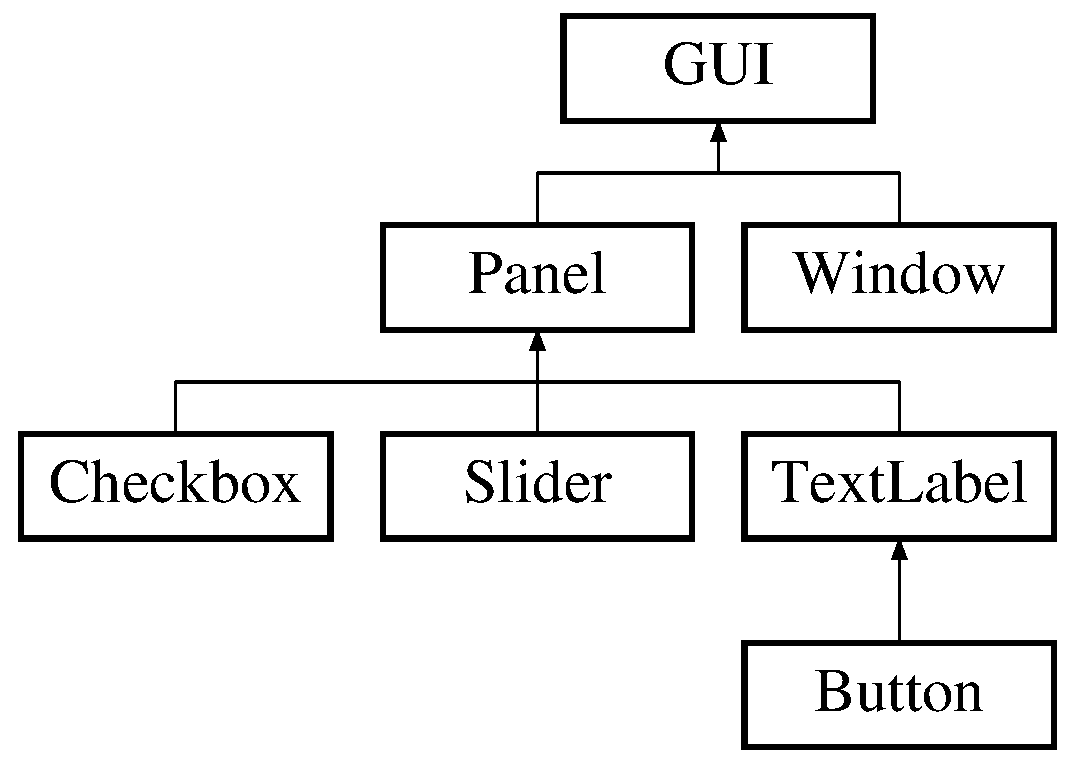
\includegraphics[height=4.000000cm]{class_g_u_i}
\end{center}
\end{figure}
\subsection*{Public Member Functions}
\begin{DoxyCompactItemize}
\item 
\mbox{\Hypertarget{class_g_u_i_a7af10a4c97e3e2c7f59134458ce36d6f}\label{class_g_u_i_a7af10a4c97e3e2c7f59134458ce36d6f}} 
{\bfseries G\+UI} (float x, float y, float width, float height, std\+::optional$<$ std\+::reference\+\_\+wrapper$<$ \mbox{\hyperlink{class_shader}{Shader}} $>$$>$ shader)
\item 
\mbox{\Hypertarget{class_g_u_i_a071cf680ab23b8025b6fc92bc2ca3fb3}\label{class_g_u_i_a071cf680ab23b8025b6fc92bc2ca3fb3}} 
{\bfseries G\+UI} (const \mbox{\hyperlink{class_g_u_i}{G\+UI}} \&copy)=default
\item 
\mbox{\Hypertarget{class_g_u_i_a71a1600d17857a2e635a587abf7ced00}\label{class_g_u_i_a71a1600d17857a2e635a587abf7ced00}} 
{\bfseries G\+UI} (\mbox{\hyperlink{class_g_u_i}{G\+UI}} \&\&move)=default
\item 
\mbox{\Hypertarget{class_g_u_i_ac0b15dbc3128f1272ae678f1b2cdc89a}\label{class_g_u_i_ac0b15dbc3128f1272ae678f1b2cdc89a}} 
\mbox{\hyperlink{class_g_u_i}{G\+UI}} \& {\bfseries operator=} (const \mbox{\hyperlink{class_g_u_i}{G\+UI}} \&rhs)=default
\item 
\mbox{\Hypertarget{class_g_u_i_a947e568bf884a8798e3e368417f662c7}\label{class_g_u_i_a947e568bf884a8798e3e368417f662c7}} 
virtual void {\bfseries update} ()
\item 
\mbox{\Hypertarget{class_g_u_i_a2abe7f08a1da35af8ae006fbecea94e0}\label{class_g_u_i_a2abe7f08a1da35af8ae006fbecea94e0}} 
virtual void {\bfseries destroy} ()
\item 
\mbox{\Hypertarget{class_g_u_i_ad2a7c1ae3938ba1d6dea0142f16d6c2b}\label{class_g_u_i_ad2a7c1ae3938ba1d6dea0142f16d6c2b}} 
virtual bool {\bfseries focused} () const =0
\item 
\mbox{\Hypertarget{class_g_u_i_a7ef5287aaa630a8d1146f0d5a35b6683}\label{class_g_u_i_a7ef5287aaa630a8d1146f0d5a35b6683}} 
virtual bool {\bfseries is\+\_\+window} () const =0
\item 
\mbox{\Hypertarget{class_g_u_i_aff34edd65faff6f3e908070a2060f6b8}\label{class_g_u_i_aff34edd65faff6f3e908070a2060f6b8}} 
virtual bool {\bfseries is\+\_\+mouse\+\_\+sensitive} () const
\item 
\mbox{\Hypertarget{class_g_u_i_abbad56adda65a7176a4e0c7e260d9449}\label{class_g_u_i_abbad56adda65a7176a4e0c7e260d9449}} 
virtual float {\bfseries get\+\_\+window\+\_\+pos\+\_\+x} () const
\item 
\mbox{\Hypertarget{class_g_u_i_a34753a0119188e4b17b4b5209c795c3a}\label{class_g_u_i_a34753a0119188e4b17b4b5209c795c3a}} 
virtual float {\bfseries get\+\_\+window\+\_\+pos\+\_\+y} () const
\item 
\mbox{\Hypertarget{class_g_u_i_a933b6bc6c5288f785d50e2621ead2193}\label{class_g_u_i_a933b6bc6c5288f785d50e2621ead2193}} 
float {\bfseries get\+\_\+x} () const
\item 
\mbox{\Hypertarget{class_g_u_i_a6a33d5bbe2d6b57b7fd2d9dc141cc3ae}\label{class_g_u_i_a6a33d5bbe2d6b57b7fd2d9dc141cc3ae}} 
float {\bfseries get\+\_\+y} () const
\item 
\mbox{\Hypertarget{class_g_u_i_a3606efd6a6db43f9751110d41ec195a3}\label{class_g_u_i_a3606efd6a6db43f9751110d41ec195a3}} 
virtual float {\bfseries get\+\_\+width} () const
\item 
\mbox{\Hypertarget{class_g_u_i_a4e427bc7271c6478d98f2215349dce07}\label{class_g_u_i_a4e427bc7271c6478d98f2215349dce07}} 
virtual float {\bfseries get\+\_\+height} () const
\item 
\mbox{\Hypertarget{class_g_u_i_a677bae0d1184e72deaf25fac052a8f95}\label{class_g_u_i_a677bae0d1184e72deaf25fac052a8f95}} 
void {\bfseries set\+\_\+x} (float x)
\item 
\mbox{\Hypertarget{class_g_u_i_aad88f8d97f43cd47a4245d5dc5a49e45}\label{class_g_u_i_aad88f8d97f43cd47a4245d5dc5a49e45}} 
void {\bfseries set\+\_\+y} (float y)
\item 
\mbox{\Hypertarget{class_g_u_i_afca3eaa048f1c0f0d0348b6882480196}\label{class_g_u_i_afca3eaa048f1c0f0d0348b6882480196}} 
void {\bfseries set\+\_\+width} (float width)
\item 
\mbox{\Hypertarget{class_g_u_i_a10a086b9e69595a9d6da48eb6d20dbc1}\label{class_g_u_i_a10a086b9e69595a9d6da48eb6d20dbc1}} 
void {\bfseries set\+\_\+height} (float height)
\item 
\mbox{\Hypertarget{class_g_u_i_a62d14b39a25ab4de6ccd5c8df6dd8624}\label{class_g_u_i_a62d14b39a25ab4de6ccd5c8df6dd8624}} 
\mbox{\hyperlink{class_window}{Window}} $\ast$ {\bfseries find\+\_\+window\+\_\+parent} () const
\item 
\mbox{\Hypertarget{class_g_u_i_aacd4d5cfd38dbec244929deabf26b010}\label{class_g_u_i_aacd4d5cfd38dbec244929deabf26b010}} 
bool {\bfseries has\+\_\+window\+\_\+parent} () const
\item 
\mbox{\Hypertarget{class_g_u_i_a4c8efe5f6b75a644ada33b438560baa9}\label{class_g_u_i_a4c8efe5f6b75a644ada33b438560baa9}} 
const std\+::optional$<$ std\+::reference\+\_\+wrapper$<$ \mbox{\hyperlink{class_shader}{Shader}} $>$ $>$ \& {\bfseries get\+\_\+shader} () const
\item 
\mbox{\Hypertarget{class_g_u_i_a3e5c5758569b0a6f7f8a0763ac5f2d56}\label{class_g_u_i_a3e5c5758569b0a6f7f8a0763ac5f2d56}} 
bool {\bfseries has\+\_\+shader} () const
\item 
\mbox{\Hypertarget{class_g_u_i_af134d9b5a265ad8996d1bea642fd06b9}\label{class_g_u_i_af134d9b5a265ad8996d1bea642fd06b9}} 
\mbox{\hyperlink{class_g_u_i}{G\+UI}} $\ast$ {\bfseries get\+\_\+parent} () const
\item 
\mbox{\Hypertarget{class_g_u_i_a5d14a0bdad4c542b854951d3092bcea2}\label{class_g_u_i_a5d14a0bdad4c542b854951d3092bcea2}} 
void {\bfseries set\+\_\+parent} (\mbox{\hyperlink{class_g_u_i}{G\+UI}} $\ast$parent)
\item 
\mbox{\Hypertarget{class_g_u_i_a680f20f016eadb403939f14dd5a820dc}\label{class_g_u_i_a680f20f016eadb403939f14dd5a820dc}} 
const std\+::deque$<$ \mbox{\hyperlink{class_g_u_i}{G\+UI}} $\ast$ $>$ \& {\bfseries get\+\_\+children} () const
\item 
\mbox{\Hypertarget{class_g_u_i_a05ceaea0a9ae997ad62f5115b32dd287}\label{class_g_u_i_a05ceaea0a9ae997ad62f5115b32dd287}} 
void {\bfseries add\+\_\+child} (\mbox{\hyperlink{class_g_u_i}{G\+UI}} $\ast$child)
\item 
\mbox{\Hypertarget{class_g_u_i_a8db69179e2a985c144c94803eddb245e}\label{class_g_u_i_a8db69179e2a985c144c94803eddb245e}} 
void {\bfseries remove\+\_\+child} (\mbox{\hyperlink{class_g_u_i}{G\+UI}} $\ast$child)
\item 
\mbox{\Hypertarget{class_g_u_i_a39a7e284ade3ed1cb65c6d22f55a80a2}\label{class_g_u_i_a39a7e284ade3ed1cb65c6d22f55a80a2}} 
bool {\bfseries is\+\_\+hidden} () const
\item 
\mbox{\Hypertarget{class_g_u_i_a6400061907f3bba6fa465238e4d94ed1}\label{class_g_u_i_a6400061907f3bba6fa465238e4d94ed1}} 
virtual void {\bfseries set\+\_\+hidden} (bool hidden)
\item 
\mbox{\Hypertarget{class_g_u_i_abb013debfa5f24e41990869f6684c228}\label{class_g_u_i_abb013debfa5f24e41990869f6684c228}} 
void {\bfseries set\+\_\+using\+\_\+proportional\+\_\+positioning} (bool use\+\_\+proportional\+\_\+positioning)
\item 
\mbox{\Hypertarget{class_g_u_i_a82dd699bec9d845e5bde59f515858f50}\label{class_g_u_i_a82dd699bec9d845e5bde59f515858f50}} 
bool {\bfseries is\+\_\+using\+\_\+proportional\+\_\+positioning} () const
\item 
\mbox{\Hypertarget{class_g_u_i_a9f8f70693f5ea986fbbdfe0686f6b30d}\label{class_g_u_i_a9f8f70693f5ea986fbbdfe0686f6b30d}} 
\mbox{\hyperlink{class_g_u_i}{G\+UI}} $\ast$ {\bfseries covered\+\_\+by} () const
\item 
\mbox{\Hypertarget{class_g_u_i_a824033514dfb2c193a5c22370a3b8fb1}\label{class_g_u_i_a824033514dfb2c193a5c22370a3b8fb1}} 
bool {\bfseries covered} () const
\end{DoxyCompactItemize}
\subsection*{Protected Attributes}
\begin{DoxyCompactItemize}
\item 
\mbox{\Hypertarget{class_g_u_i_a7fa193a8ffb27bbb3bcc225e36f6d54d}\label{class_g_u_i_a7fa193a8ffb27bbb3bcc225e36f6d54d}} 
float {\bfseries x}
\item 
\mbox{\Hypertarget{class_g_u_i_a98f204f99ffc5ff6cffc9340bbb8c29b}\label{class_g_u_i_a98f204f99ffc5ff6cffc9340bbb8c29b}} 
float {\bfseries y}
\item 
\mbox{\Hypertarget{class_g_u_i_aee5d8766834f6f743f0d8b8c16e47155}\label{class_g_u_i_aee5d8766834f6f743f0d8b8c16e47155}} 
float {\bfseries width}
\item 
\mbox{\Hypertarget{class_g_u_i_a70b578c36323a45cac88ccff3bced933}\label{class_g_u_i_a70b578c36323a45cac88ccff3bced933}} 
float {\bfseries height}
\item 
\mbox{\Hypertarget{class_g_u_i_a64b007b31d0ec8a8704f9ab3bb2a7d3d}\label{class_g_u_i_a64b007b31d0ec8a8704f9ab3bb2a7d3d}} 
std\+::optional$<$ std\+::reference\+\_\+wrapper$<$ \mbox{\hyperlink{class_shader}{Shader}} $>$ $>$ {\bfseries shader}
\item 
\mbox{\Hypertarget{class_g_u_i_ac9c33263556b3c9997f9c7b360f06a93}\label{class_g_u_i_ac9c33263556b3c9997f9c7b360f06a93}} 
\mbox{\hyperlink{class_g_u_i}{G\+UI}} $\ast$ {\bfseries parent}
\item 
\mbox{\Hypertarget{class_g_u_i_a2ff82067e32c06d5ba9b6aa4d860666a}\label{class_g_u_i_a2ff82067e32c06d5ba9b6aa4d860666a}} 
std\+::deque$<$ \mbox{\hyperlink{class_g_u_i}{G\+UI}} $\ast$ $>$ {\bfseries children}
\item 
\mbox{\Hypertarget{class_g_u_i_a270e03faf2f4612883700dc89ec7e0d0}\label{class_g_u_i_a270e03faf2f4612883700dc89ec7e0d0}} 
bool {\bfseries hidden}
\item 
\mbox{\Hypertarget{class_g_u_i_a6b75b1bd88f2e04e919a4a9f2333f634}\label{class_g_u_i_a6b75b1bd88f2e04e919a4a9f2333f634}} 
bool {\bfseries use\+\_\+proportional\+\_\+positioning}
\end{DoxyCompactItemize}


\subsection{Detailed Description}
Represents a Topaz \mbox{\hyperlink{class_g_u_i}{G\+UI}} element. Abstract. Not available for non-\/polymorphic use. Inherit from this to create custom Topaz \mbox{\hyperlink{class_g_u_i}{G\+UI}} yourself. 

The documentation for this class was generated from the following files\+:\begin{DoxyCompactItemize}
\item 
src/graphics/gui.\+hpp\item 
src/graphics/gui.\+cpp\end{DoxyCompactItemize}

\hypertarget{classtz_1_1graphics_1_1model_1_1_indexed_model}{}\section{tz\+:\+:graphics\+:\+:model\+:\+:Indexed\+Model Class Reference}
\label{classtz_1_1graphics_1_1model_1_1_indexed_model}\index{tz\+::graphics\+::model\+::\+Indexed\+Model@{tz\+::graphics\+::model\+::\+Indexed\+Model}}


{\ttfamily \#include $<$graphics.\+hpp$>$}

\subsection*{Public Member Functions}
\begin{DoxyCompactItemize}
\item 
void \mbox{\hyperlink{classtz_1_1graphics_1_1model_1_1_indexed_model_a019b4f8c72e1e7dd37d2d3ec452cfa3b}{calculate\+\_\+normals}} ()
\item 
void \mbox{\hyperlink{classtz_1_1graphics_1_1model_1_1_indexed_model_ae5dae45074924bcdfbc2adf2ec13f0ec}{calculate\+\_\+tangents}} ()
\end{DoxyCompactItemize}
\subsection*{Public Attributes}
\begin{DoxyCompactItemize}
\item 
\mbox{\Hypertarget{classtz_1_1graphics_1_1model_1_1_indexed_model_ae94e4a6c4f1dc9bac6c003eda93d849f}\label{classtz_1_1graphics_1_1model_1_1_indexed_model_ae94e4a6c4f1dc9bac6c003eda93d849f}} 
std\+::vector$<$ \mbox{\hyperlink{class_vector3}{Vector3F}} $>$ \mbox{\hyperlink{classtz_1_1graphics_1_1model_1_1_indexed_model_ae94e4a6c4f1dc9bac6c003eda93d849f}{positions}}
\begin{DoxyCompactList}\small\item\em Container for all \mbox{\hyperlink{class_vertex}{Vertex}} positions. Each position is in model-\/space. \end{DoxyCompactList}\item 
\mbox{\Hypertarget{classtz_1_1graphics_1_1model_1_1_indexed_model_a51345de6dc0c2773d503a367a07c9456}\label{classtz_1_1graphics_1_1model_1_1_indexed_model_a51345de6dc0c2773d503a367a07c9456}} 
std\+::vector$<$ \mbox{\hyperlink{class_vector2}{Vector2F}} $>$ \mbox{\hyperlink{classtz_1_1graphics_1_1model_1_1_indexed_model_a51345de6dc0c2773d503a367a07c9456}{texcoords}}
\begin{DoxyCompactList}\small\item\em Container for all \mbox{\hyperlink{class_vertex}{Vertex}} texture-\/coordinates (U\+Vs). \end{DoxyCompactList}\item 
\mbox{\Hypertarget{classtz_1_1graphics_1_1model_1_1_indexed_model_a4a9e2cc61d38cb598ae00acb771bd58e}\label{classtz_1_1graphics_1_1model_1_1_indexed_model_a4a9e2cc61d38cb598ae00acb771bd58e}} 
std\+::vector$<$ \mbox{\hyperlink{class_vector3}{Vector3F}} $>$ \mbox{\hyperlink{classtz_1_1graphics_1_1model_1_1_indexed_model_a4a9e2cc61d38cb598ae00acb771bd58e}{normals}}
\begin{DoxyCompactList}\small\item\em Container for all \mbox{\hyperlink{class_vertex}{Vertex}} normal Vectors. \end{DoxyCompactList}\item 
\mbox{\Hypertarget{classtz_1_1graphics_1_1model_1_1_indexed_model_affe23c0f119019eed8e95f09c4404131}\label{classtz_1_1graphics_1_1model_1_1_indexed_model_affe23c0f119019eed8e95f09c4404131}} 
std\+::vector$<$ \mbox{\hyperlink{class_vector3}{Vector3F}} $>$ \mbox{\hyperlink{classtz_1_1graphics_1_1model_1_1_indexed_model_affe23c0f119019eed8e95f09c4404131}{tangents}}
\begin{DoxyCompactList}\small\item\em Container for all \mbox{\hyperlink{class_vertex}{Vertex}} tangent Vectors. \end{DoxyCompactList}\item 
\mbox{\Hypertarget{classtz_1_1graphics_1_1model_1_1_indexed_model_a1b87b564e60fdb25df24515567fa4040}\label{classtz_1_1graphics_1_1model_1_1_indexed_model_a1b87b564e60fdb25df24515567fa4040}} 
std\+::vector$<$ unsigned int $>$ \mbox{\hyperlink{classtz_1_1graphics_1_1model_1_1_indexed_model_a1b87b564e60fdb25df24515567fa4040}{indices}}
\begin{DoxyCompactList}\small\item\em Container for all \mbox{\hyperlink{class_vertex}{Vertex}} indices. \end{DoxyCompactList}\end{DoxyCompactItemize}


\subsection{Detailed Description}
Barebones representation of a 3D model. 

\subsection{Member Function Documentation}
\mbox{\Hypertarget{classtz_1_1graphics_1_1model_1_1_indexed_model_a019b4f8c72e1e7dd37d2d3ec452cfa3b}\label{classtz_1_1graphics_1_1model_1_1_indexed_model_a019b4f8c72e1e7dd37d2d3ec452cfa3b}} 
\index{tz\+::graphics\+::model\+::\+Indexed\+Model@{tz\+::graphics\+::model\+::\+Indexed\+Model}!calculate\+\_\+normals@{calculate\+\_\+normals}}
\index{calculate\+\_\+normals@{calculate\+\_\+normals}!tz\+::graphics\+::model\+::\+Indexed\+Model@{tz\+::graphics\+::model\+::\+Indexed\+Model}}
\subsubsection{\texorpdfstring{calculate\+\_\+normals()}{calculate\_normals()}}
{\footnotesize\ttfamily void tz\+::graphics\+::model\+::\+Indexed\+Model\+::calculate\+\_\+normals (\begin{DoxyParamCaption}{ }\end{DoxyParamCaption})}

Calculate and populate the container for all \mbox{\hyperlink{class_vertex}{Vertex}} normal Vectors. \mbox{\Hypertarget{classtz_1_1graphics_1_1model_1_1_indexed_model_ae5dae45074924bcdfbc2adf2ec13f0ec}\label{classtz_1_1graphics_1_1model_1_1_indexed_model_ae5dae45074924bcdfbc2adf2ec13f0ec}} 
\index{tz\+::graphics\+::model\+::\+Indexed\+Model@{tz\+::graphics\+::model\+::\+Indexed\+Model}!calculate\+\_\+tangents@{calculate\+\_\+tangents}}
\index{calculate\+\_\+tangents@{calculate\+\_\+tangents}!tz\+::graphics\+::model\+::\+Indexed\+Model@{tz\+::graphics\+::model\+::\+Indexed\+Model}}
\subsubsection{\texorpdfstring{calculate\+\_\+tangents()}{calculate\_tangents()}}
{\footnotesize\ttfamily void tz\+::graphics\+::model\+::\+Indexed\+Model\+::calculate\+\_\+tangents (\begin{DoxyParamCaption}{ }\end{DoxyParamCaption})}

Calculate the populate the container for all \mbox{\hyperlink{class_vertex}{Vertex}} tangent Vectors. 

The documentation for this class was generated from the following files\+:\begin{DoxyCompactItemize}
\item 
src/graphics/graphics.\+hpp\item 
src/graphics/graphics.\+cpp\end{DoxyCompactItemize}

\hypertarget{class_instanced_mesh}{}\section{Instanced\+Mesh Class Reference}
\label{class_instanced_mesh}\index{Instanced\+Mesh@{Instanced\+Mesh}}


{\ttfamily \#include $<$mesh.\+hpp$>$}

Inheritance diagram for Instanced\+Mesh\+:\begin{figure}[H]
\begin{center}
\leavevmode
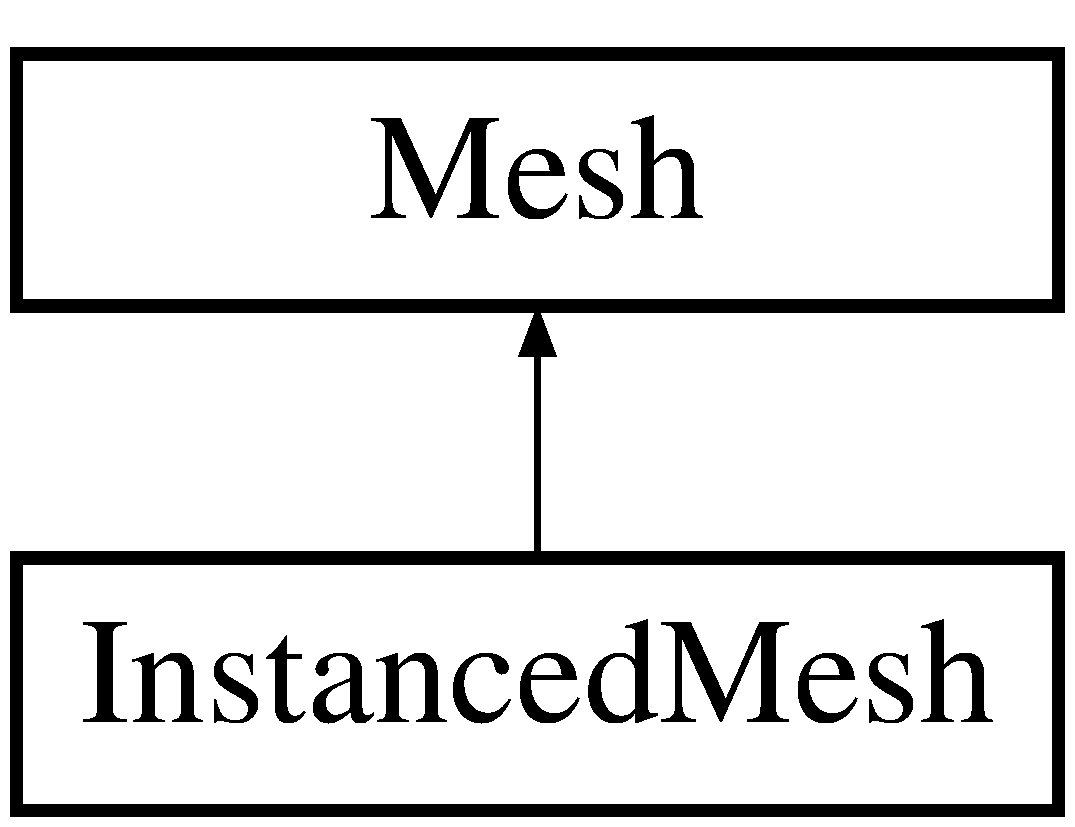
\includegraphics[height=2.000000cm]{class_instanced_mesh}
\end{center}
\end{figure}
\subsection*{Public Member Functions}
\begin{DoxyCompactItemize}
\item 
\mbox{\Hypertarget{class_instanced_mesh_a21071278154b9446677016224861bffd}\label{class_instanced_mesh_a21071278154b9446677016224861bffd}} 
{\bfseries Instanced\+Mesh} (std\+::string filename, std\+::vector$<$ \mbox{\hyperlink{class_vector3}{Vector3F}} $>$ positions, std\+::vector$<$ \mbox{\hyperlink{class_vector3}{Vector3F}} $>$ rotations, std\+::vector$<$ \mbox{\hyperlink{class_vector3}{Vector3F}} $>$ scales)
\item 
\mbox{\Hypertarget{class_instanced_mesh_a3457a47b5d850fbdae6b49a8d4bfadd1}\label{class_instanced_mesh_a3457a47b5d850fbdae6b49a8d4bfadd1}} 
{\bfseries Instanced\+Mesh} (const \mbox{\hyperlink{class_instanced_mesh}{Instanced\+Mesh}} \&copy)=default
\item 
\mbox{\Hypertarget{class_instanced_mesh_abdc6da71131053efc82bd3377aabc1ac}\label{class_instanced_mesh_abdc6da71131053efc82bd3377aabc1ac}} 
{\bfseries Instanced\+Mesh} (\mbox{\hyperlink{class_instanced_mesh}{Instanced\+Mesh}} \&\&move)=default
\item 
\mbox{\Hypertarget{class_instanced_mesh_afce42cfdb1ff1abcd70c418fd0dd0503}\label{class_instanced_mesh_afce42cfdb1ff1abcd70c418fd0dd0503}} 
\mbox{\hyperlink{class_instanced_mesh}{Instanced\+Mesh}} \& {\bfseries operator=} (const \mbox{\hyperlink{class_instanced_mesh}{Instanced\+Mesh}} \&rhs)=default
\item 
\mbox{\Hypertarget{class_instanced_mesh_afe65a816eab00c2d6217f8cd4f8d7749}\label{class_instanced_mesh_afe65a816eab00c2d6217f8cd4f8d7749}} 
const std\+::vector$<$ \mbox{\hyperlink{class_vector3}{Vector3F}} $>$ \& {\bfseries get\+\_\+instance\+\_\+positions} () const
\item 
\mbox{\Hypertarget{class_instanced_mesh_a0618a1d06d7f63edfd7d76f9d51c10de}\label{class_instanced_mesh_a0618a1d06d7f63edfd7d76f9d51c10de}} 
const std\+::vector$<$ \mbox{\hyperlink{class_vector3}{Vector3F}} $>$ \& {\bfseries get\+\_\+instance\+\_\+rotations} () const
\item 
\mbox{\Hypertarget{class_instanced_mesh_a6f3e0e63ec4dbcf7715bdb44bc83ecaa}\label{class_instanced_mesh_a6f3e0e63ec4dbcf7715bdb44bc83ecaa}} 
const std\+::vector$<$ \mbox{\hyperlink{class_vector3}{Vector3F}} $>$ \& {\bfseries get\+\_\+instance\+\_\+scales} () const
\item 
\mbox{\Hypertarget{class_instanced_mesh_af35eca32f1270f3f996f508e7cc9d01d}\label{class_instanced_mesh_af35eca32f1270f3f996f508e7cc9d01d}} 
std\+::size\+\_\+t {\bfseries get\+\_\+instance\+\_\+quantity} () const
\item 
\mbox{\Hypertarget{class_instanced_mesh_aab465896e76ef3c0b203cde8cd196e12}\label{class_instanced_mesh_aab465896e76ef3c0b203cde8cd196e12}} 
virtual void {\bfseries render} (bool patches, G\+Lenum mode=G\+L\+\_\+\+T\+R\+I\+A\+N\+G\+L\+ES) const override
\end{DoxyCompactItemize}
\subsection*{Additional Inherited Members}


\subsection{Detailed Description}
Like a normal mesh, but supports Open\+GL instancing. Use this if you want to render the same mesh very many times at once with little attribute changes. This class is abstracted away by tz\+::graphics\+::batch in \mbox{\hyperlink{object_8hpp_source}{object.\+hpp}}. 

The documentation for this class was generated from the following files\+:\begin{DoxyCompactItemize}
\item 
src/graphics/mesh.\+hpp\item 
src/graphics/mesh.\+cpp\end{DoxyCompactItemize}

\hypertarget{class_key_listener}{}\section{Key\+Listener Class Reference}
\label{class_key_listener}\index{Key\+Listener@{Key\+Listener}}


{\ttfamily \#include $<$listener.\+hpp$>$}

Inheritance diagram for Key\+Listener\+:\begin{figure}[H]
\begin{center}
\leavevmode
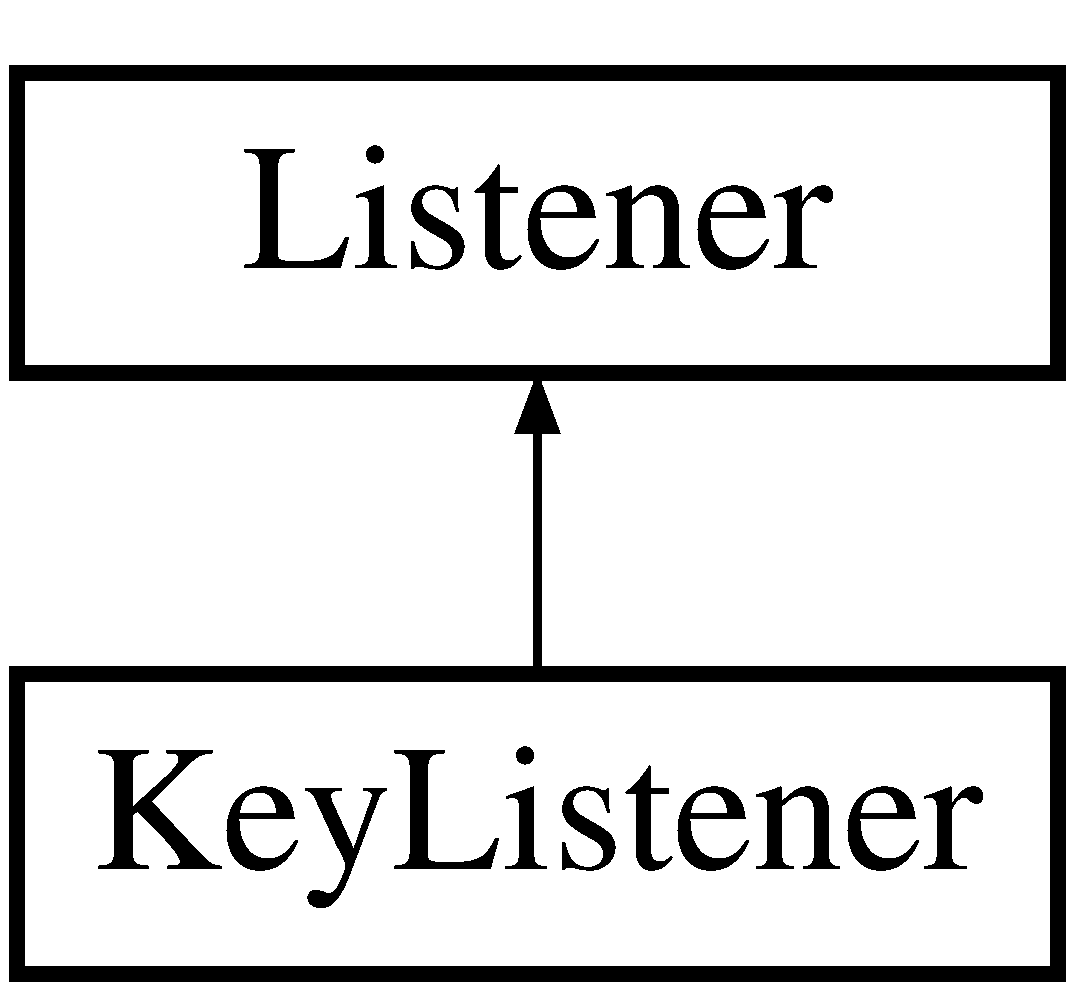
\includegraphics[height=2.000000cm]{class_key_listener}
\end{center}
\end{figure}
\subsection*{Public Member Functions}
\begin{DoxyCompactItemize}
\item 
\mbox{\Hypertarget{class_key_listener_ab916f7cf930c921ab0a7979fa7234056}\label{class_key_listener_ab916f7cf930c921ab0a7979fa7234056}} 
{\bfseries Key\+Listener} (\mbox{\hyperlink{class_window}{Window}} \&window)
\item 
\mbox{\Hypertarget{class_key_listener_a77e112bbf7e34dfb9c4d65ad96496389}\label{class_key_listener_a77e112bbf7e34dfb9c4d65ad96496389}} 
{\bfseries Key\+Listener} (const \mbox{\hyperlink{class_key_listener}{Key\+Listener}} \&copy)=default
\item 
\mbox{\Hypertarget{class_key_listener_aebb1bc88efca72921f3740911c20fa30}\label{class_key_listener_aebb1bc88efca72921f3740911c20fa30}} 
{\bfseries Key\+Listener} (\mbox{\hyperlink{class_key_listener}{Key\+Listener}} \&\&move)=default
\item 
\mbox{\Hypertarget{class_key_listener_a95a92bca7d105dd906be81613798cdd2}\label{class_key_listener_a95a92bca7d105dd906be81613798cdd2}} 
\mbox{\hyperlink{class_key_listener}{Key\+Listener}} \& {\bfseries operator=} (const \mbox{\hyperlink{class_key_listener}{Key\+Listener}} \&rhs)=default
\item 
\mbox{\Hypertarget{class_key_listener_a2a7de72fe731c72f125560060db2c765}\label{class_key_listener_a2a7de72fe731c72f125560060db2c765}} 
virtual void {\bfseries handle\+\_\+events} (S\+D\+L\+\_\+\+Event \&evt) override
\item 
\mbox{\Hypertarget{class_key_listener_ab83113043164890f27fea24bca103dd6}\label{class_key_listener_ab83113043164890f27fea24bca103dd6}} 
bool {\bfseries is\+\_\+key\+\_\+pressed} (const std\+::string \&keyname) const
\item 
\mbox{\Hypertarget{class_key_listener_ad2a4b0a94d69949b2bb8d83b3e937d80}\label{class_key_listener_ad2a4b0a94d69949b2bb8d83b3e937d80}} 
bool {\bfseries is\+\_\+key\+\_\+released} (const std\+::string \&keyname) const
\item 
\mbox{\Hypertarget{class_key_listener_a55024ee26dd4ca72d4ce0b0c3b381235}\label{class_key_listener_a55024ee26dd4ca72d4ce0b0c3b381235}} 
bool {\bfseries catch\+\_\+key\+\_\+pressed} (const std\+::string \&keyname)
\item 
\mbox{\Hypertarget{class_key_listener_a01406b86c1607891068a0b2f65305048}\label{class_key_listener_a01406b86c1607891068a0b2f65305048}} 
bool {\bfseries catch\+\_\+key\+\_\+released} (const std\+::string \&keyname)
\end{DoxyCompactItemize}
\subsection*{Additional Inherited Members}


\subsection{Detailed Description}
How Topaz handles keyboard input. Register this to a Topaz \mbox{\hyperlink{class_window}{Window}} to use properly. 

The documentation for this class was generated from the following files\+:\begin{DoxyCompactItemize}
\item 
src/listener.\+hpp\item 
src/listener.\+cpp\end{DoxyCompactItemize}

\hypertarget{class_listener}{}\section{Listener Class Reference}
\label{class_listener}\index{Listener@{Listener}}


{\ttfamily \#include $<$listener.\+hpp$>$}

Inheritance diagram for Listener\+:\begin{figure}[H]
\begin{center}
\leavevmode
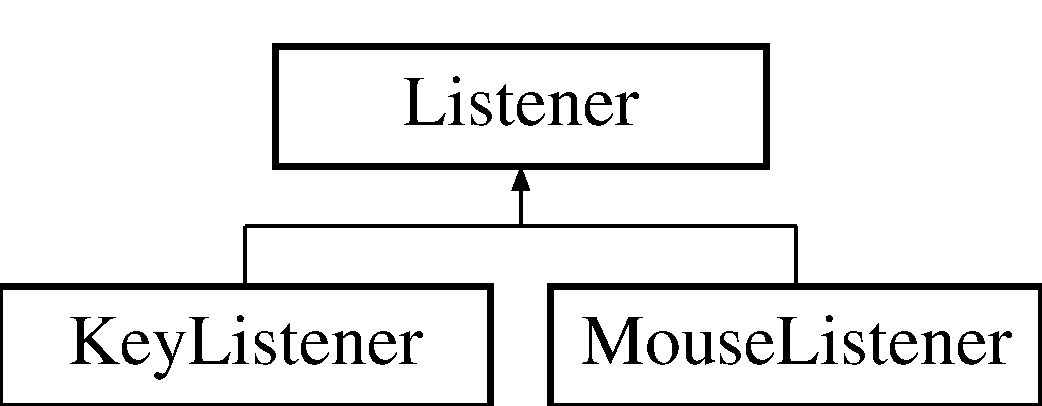
\includegraphics[height=2.000000cm]{class_listener}
\end{center}
\end{figure}
\subsection*{Public Member Functions}
\begin{DoxyCompactItemize}
\item 
\mbox{\Hypertarget{class_listener_ab3e6483c6f473dd9700211743afb294a}\label{class_listener_ab3e6483c6f473dd9700211743afb294a}} 
{\bfseries Listener} (const \mbox{\hyperlink{class_listener}{Listener}} \&copy)=default
\item 
\mbox{\Hypertarget{class_listener_a606eefbf88f0a072290bb7f3df891e63}\label{class_listener_a606eefbf88f0a072290bb7f3df891e63}} 
{\bfseries Listener} (\mbox{\hyperlink{class_listener}{Listener}} \&\&move)=default
\item 
\mbox{\Hypertarget{class_listener_aa73bdc3ee858635ea38633543c665b0e}\label{class_listener_aa73bdc3ee858635ea38633543c665b0e}} 
\mbox{\hyperlink{class_listener}{Listener}} \& {\bfseries operator=} (const \mbox{\hyperlink{class_listener}{Listener}} \&rhs)=default
\item 
\mbox{\Hypertarget{class_listener_a23fc6d7a14eaa5891813b98794ab0fcf}\label{class_listener_a23fc6d7a14eaa5891813b98794ab0fcf}} 
virtual void {\bfseries handle\+\_\+events} (S\+D\+L\+\_\+\+Event \&evt)=0
\item 
\mbox{\Hypertarget{class_listener_a7f028341ab1458b8c1a6d44e8fc1e0f1}\label{class_listener_a7f028341ab1458b8c1a6d44e8fc1e0f1}} 
unsigned int {\bfseries get\+\_\+id} () const
\end{DoxyCompactItemize}
\subsection*{Static Public Member Functions}
\begin{DoxyCompactItemize}
\item 
\mbox{\Hypertarget{class_listener_a6c783b3b1febd9f9c1b5200b0bb470e4}\label{class_listener_a6c783b3b1febd9f9c1b5200b0bb470e4}} 
static unsigned int {\bfseries get\+\_\+num\+\_\+listeners} ()
\end{DoxyCompactItemize}


\subsection{Detailed Description}
Wrapper for an S\+D\+L\+\_\+\+Event listener. Abstract. Not available for non-\/polymorphic use. Inherit from this to create custom listeners that a Topaz \mbox{\hyperlink{class_window}{Window}} can register. 

The documentation for this class was generated from the following files\+:\begin{DoxyCompactItemize}
\item 
src/listener.\+hpp\item 
src/listener.\+cpp\end{DoxyCompactItemize}

\hypertarget{classtz_1_1data_1_1_manager}{}\section{tz\+:\+:data\+:\+:Manager Class Reference}
\label{classtz_1_1data_1_1_manager}\index{tz\+::data\+::\+Manager@{tz\+::data\+::\+Manager}}


{\ttfamily \#include $<$data.\+hpp$>$}

\subsection*{Public Member Functions}
\begin{DoxyCompactItemize}
\item 
\mbox{\Hypertarget{classtz_1_1data_1_1_manager_a193453bb8103989bc0470c0bc92aaacc}\label{classtz_1_1data_1_1_manager_a193453bb8103989bc0470c0bc92aaacc}} 
{\bfseries Manager} (std\+::string datafilename)
\item 
\mbox{\Hypertarget{classtz_1_1data_1_1_manager_a0ff2e0652aff2156ffefe0407c3de01a}\label{classtz_1_1data_1_1_manager_a0ff2e0652aff2156ffefe0407c3de01a}} 
{\bfseries Manager} (const \mbox{\hyperlink{classtz_1_1data_1_1_manager}{Manager}} \&copy)=default
\item 
\mbox{\Hypertarget{classtz_1_1data_1_1_manager_a4d643fbbf4567894eab938269d8b8018}\label{classtz_1_1data_1_1_manager_a4d643fbbf4567894eab938269d8b8018}} 
{\bfseries Manager} (\mbox{\hyperlink{classtz_1_1data_1_1_manager}{Manager}} \&\&move)=default
\item 
\mbox{\Hypertarget{classtz_1_1data_1_1_manager_a941a0cdd736b9d0baebf2ce69f6164bd}\label{classtz_1_1data_1_1_manager_a941a0cdd736b9d0baebf2ce69f6164bd}} 
\mbox{\hyperlink{classtz_1_1data_1_1_manager}{Manager}} \& {\bfseries operator=} (const \mbox{\hyperlink{classtz_1_1data_1_1_manager}{Manager}} \&rhs)=default
\item 
\mbox{\Hypertarget{classtz_1_1data_1_1_manager_a2e8da95d6b61f144b27e385c4d5d6e19}\label{classtz_1_1data_1_1_manager_a2e8da95d6b61f144b27e385c4d5d6e19}} 
std\+::string {\bfseries resource\+\_\+link} (const std\+::string \&resource\+\_\+name) const
\item 
\mbox{\Hypertarget{classtz_1_1data_1_1_manager_a5282c9de3f5363f64ff370545b5dc37d}\label{classtz_1_1data_1_1_manager_a5282c9de3f5363f64ff370545b5dc37d}} 
std\+::string {\bfseries resource\+\_\+name} (const std\+::string \&resource\+\_\+link) const
\item 
\mbox{\Hypertarget{classtz_1_1data_1_1_manager_a84a45f4d8a495b3d9e73fb65ecb9bdbd}\label{classtz_1_1data_1_1_manager_a84a45f4d8a495b3d9e73fb65ecb9bdbd}} 
std\+::unordered\+\_\+map$<$ std\+::string, std\+::string $>$ {\bfseries retrieve\+\_\+models} (const char $\ast$sequence\+\_\+name=tz\+::data\+::default\+\_\+models\+\_\+sequence\+\_\+name) const
\item 
\mbox{\Hypertarget{classtz_1_1data_1_1_manager_a34794eeba3213538092c71493ef42dda}\label{classtz_1_1data_1_1_manager_a34794eeba3213538092c71493ef42dda}} 
std\+::unordered\+\_\+map$<$ std\+::string, std\+::string $>$ {\bfseries retrieve\+\_\+textures} (const char $\ast$sequence\+\_\+name=tz\+::data\+::default\+\_\+textures\+\_\+sequence\+\_\+name) const
\item 
\mbox{\Hypertarget{classtz_1_1data_1_1_manager_a223bf9e1245c4ed253be667086fd7165}\label{classtz_1_1data_1_1_manager_a223bf9e1245c4ed253be667086fd7165}} 
std\+::unordered\+\_\+map$<$ std\+::string, std\+::string $>$ {\bfseries retrieve\+\_\+normal\+\_\+maps} (const char $\ast$sequence\+\_\+name=tz\+::data\+::default\+\_\+normal\+\_\+maps\+\_\+sequence\+\_\+name) const
\item 
\mbox{\Hypertarget{classtz_1_1data_1_1_manager_a27a9b4cd6d382f43729b7672e3ffdd99}\label{classtz_1_1data_1_1_manager_a27a9b4cd6d382f43729b7672e3ffdd99}} 
std\+::unordered\+\_\+map$<$ std\+::string, std\+::string $>$ {\bfseries retrieve\+\_\+parallax\+\_\+maps} (const char $\ast$sequence\+\_\+name=tz\+::data\+::default\+\_\+parallax\+\_\+maps\+\_\+sequence\+\_\+name) const
\item 
\mbox{\Hypertarget{classtz_1_1data_1_1_manager_a8ea220b62bc50df0cad8ecf4a2c8102f}\label{classtz_1_1data_1_1_manager_a8ea220b62bc50df0cad8ecf4a2c8102f}} 
std\+::unordered\+\_\+map$<$ std\+::string, std\+::string $>$ {\bfseries retrieve\+\_\+displacement\+\_\+maps} (const char $\ast$sequence\+\_\+name=tz\+::data\+::default\+\_\+displacement\+\_\+maps\+\_\+sequence\+\_\+name) const
\item 
\mbox{\Hypertarget{classtz_1_1data_1_1_manager_a22fe43e7c985db9adbadc2be1c6ab5cd}\label{classtz_1_1data_1_1_manager_a22fe43e7c985db9adbadc2be1c6ab5cd}} 
unsigned int {\bfseries retrieve\+\_\+all\+\_\+data} (std\+::vector$<$ std\+::unique\+\_\+ptr$<$ \mbox{\hyperlink{class_mesh}{Mesh}} $>$$>$ \&all\+\_\+meshes, std\+::vector$<$ std\+::unique\+\_\+ptr$<$ \mbox{\hyperlink{class_texture}{Texture}} $>$$>$ \&all\+\_\+textures, std\+::vector$<$ std\+::unique\+\_\+ptr$<$ \mbox{\hyperlink{class_normal_map}{Normal\+Map}} $>$$>$ \&all\+\_\+normalmaps, std\+::vector$<$ std\+::unique\+\_\+ptr$<$ \mbox{\hyperlink{class_parallax_map}{Parallax\+Map}} $>$$>$ \&all\+\_\+parallaxmaps, std\+::vector$<$ std\+::unique\+\_\+ptr$<$ \mbox{\hyperlink{class_displacement_map}{Displacement\+Map}} $>$$>$ \&all\+\_\+displacementmaps) const
\end{DoxyCompactItemize}


\subsection{Detailed Description}
Essentially an M\+DL Asset \mbox{\hyperlink{classtz_1_1data_1_1_manager}{Manager}}. This is how Topaz handles M\+DL data files which hold assets such as textures and models. 

The documentation for this class was generated from the following files\+:\begin{DoxyCompactItemize}
\item 
src/data.\+hpp\item 
src/data.\+cpp\end{DoxyCompactItemize}

\hypertarget{class_material}{}\section{Material Class Reference}
\label{class_material}\index{Material@{Material}}


{\ttfamily \#include $<$material.\+hpp$>$}

\subsection*{Public Member Functions}
\begin{DoxyCompactItemize}
\item 
\mbox{\Hypertarget{class_material_a5f13270a309ddc1805fb8debe6a9ca55}\label{class_material_a5f13270a309ddc1805fb8debe6a9ca55}} 
{\bfseries Material} (\mbox{\hyperlink{class_texture}{Texture}} $\ast$texture, \mbox{\hyperlink{class_normal_map}{Normal\+Map}} $\ast$normal\+\_\+map=nullptr, \mbox{\hyperlink{class_parallax_map}{Parallax\+Map}} $\ast$parallax\+\_\+map=nullptr, \mbox{\hyperlink{class_displacement_map}{Displacement\+Map}} $\ast$displacement\+\_\+map=nullptr)
\item 
bool \mbox{\hyperlink{class_material_a2cbd77887660ea994ff3212d5630d575}{has\+\_\+texture}} () const
\item 
\mbox{\Hypertarget{class_material_a75d9771927c46c10299088d960da291a}\label{class_material_a75d9771927c46c10299088d960da291a}} 
const \mbox{\hyperlink{class_texture}{Texture}} $\ast$ {\bfseries get\+\_\+texture} () const
\item 
\mbox{\Hypertarget{class_material_a8a1b4f058fec07fff599f09fc666792c}\label{class_material_a8a1b4f058fec07fff599f09fc666792c}} 
bool {\bfseries has\+\_\+normal\+\_\+map} () const
\item 
\mbox{\Hypertarget{class_material_a202edfb1421c3731262e0020d01afa01}\label{class_material_a202edfb1421c3731262e0020d01afa01}} 
const \mbox{\hyperlink{class_normal_map}{Normal\+Map}} $\ast$ {\bfseries get\+\_\+normal\+\_\+map} () const
\item 
\mbox{\Hypertarget{class_material_ae16d88f71df7097c161fe0ced7d26bf3}\label{class_material_ae16d88f71df7097c161fe0ced7d26bf3}} 
bool {\bfseries has\+\_\+parallax\+\_\+map} () const
\item 
\mbox{\Hypertarget{class_material_a757210ff3a350f629999464e8fd518b6}\label{class_material_a757210ff3a350f629999464e8fd518b6}} 
const \mbox{\hyperlink{class_parallax_map}{Parallax\+Map}} $\ast$ {\bfseries get\+\_\+parallax\+\_\+map} () const
\item 
\mbox{\Hypertarget{class_material_a02a7a36f8914ab673c956f72f2567099}\label{class_material_a02a7a36f8914ab673c956f72f2567099}} 
bool {\bfseries has\+\_\+displacement\+\_\+map} () const
\item 
\mbox{\Hypertarget{class_material_a13740af80c449e957271d6a47db93c44}\label{class_material_a13740af80c449e957271d6a47db93c44}} 
const \mbox{\hyperlink{class_displacement_map}{Displacement\+Map}} $\ast$ {\bfseries get\+\_\+displacement\+\_\+map} () const
\item 
\mbox{\Hypertarget{class_material_a249d65e23e1b214c13d8ff3b60abd2db}\label{class_material_a249d65e23e1b214c13d8ff3b60abd2db}} 
void {\bfseries set\+\_\+texture} (\mbox{\hyperlink{class_texture}{Texture}} $\ast$texture)
\item 
\mbox{\Hypertarget{class_material_a0a3f8735d6b8843cd4a7c3f598a147de}\label{class_material_a0a3f8735d6b8843cd4a7c3f598a147de}} 
void {\bfseries set\+\_\+normal\+\_\+map} (\mbox{\hyperlink{class_normal_map}{Normal\+Map}} $\ast$normal\+\_\+map)
\item 
\mbox{\Hypertarget{class_material_a8f324d2f579e680798ec07527446a525}\label{class_material_a8f324d2f579e680798ec07527446a525}} 
void {\bfseries set\+\_\+parallax\+\_\+map} (\mbox{\hyperlink{class_parallax_map}{Parallax\+Map}} $\ast$parallax\+\_\+map)
\item 
\mbox{\Hypertarget{class_material_a292bc6429310ce4db4a1282d40aca36c}\label{class_material_a292bc6429310ce4db4a1282d40aca36c}} 
void {\bfseries set\+\_\+displacement\+\_\+map} (\mbox{\hyperlink{class_displacement_map}{Displacement\+Map}} $\ast$displacement\+\_\+map)
\item 
\mbox{\Hypertarget{class_material_a0053a121698c3c5af8e889204d3b80cf}\label{class_material_a0053a121698c3c5af8e889204d3b80cf}} 
virtual void {\bfseries bind} (\mbox{\hyperlink{class_shader}{Shader}} \&shader) const
\item 
\mbox{\Hypertarget{class_material_aa0519b7438e5ebdcc86d17817c96016d}\label{class_material_aa0519b7438e5ebdcc86d17817c96016d}} 
bool {\bfseries operator==} (const \mbox{\hyperlink{class_material}{Material}} \&rhs) const
\end{DoxyCompactItemize}


\subsection{Detailed Description}
Non-\/owning container for a tuple of \mbox{\hyperlink{class_texture}{Texture}}, \mbox{\hyperlink{class_normal_map}{Normal\+Map}}, \mbox{\hyperlink{class_parallax_map}{Parallax\+Map}} and \mbox{\hyperlink{class_displacement_map}{Displacement\+Map}}. Objects contain one of these for simplity\textquotesingle{}s sake. 

\subsection{Member Function Documentation}
\mbox{\Hypertarget{class_material_a2cbd77887660ea994ff3212d5630d575}\label{class_material_a2cbd77887660ea994ff3212d5630d575}} 
\index{Material@{Material}!has\+\_\+texture@{has\+\_\+texture}}
\index{has\+\_\+texture@{has\+\_\+texture}!Material@{Material}}
\subsubsection{\texorpdfstring{has\+\_\+texture()}{has\_texture()}}
{\footnotesize\ttfamily bool Material\+::has\+\_\+texture (\begin{DoxyParamCaption}{ }\end{DoxyParamCaption}) const}

Returns true if the texture component is not null. Note\+: This will return false if the default-\/texture was manually passed into the constructor, but true if nullptr was passed and the default-\/texture was inferred. 

The documentation for this class was generated from the following files\+:\begin{DoxyCompactItemize}
\item 
src/graphics/material.\+hpp\item 
src/graphics/material.\+cpp\end{DoxyCompactItemize}

\hypertarget{class_matrix2x2}{}\section{Matrix2x2 Class Reference}
\label{class_matrix2x2}\index{Matrix2x2@{Matrix2x2}}


{\ttfamily \#include $<$matrix.\+hpp$>$}

\subsection*{Public Member Functions}
\begin{DoxyCompactItemize}
\item 
\mbox{\Hypertarget{class_matrix2x2_a862d6eb13040d4e06b5cd16de42425bb}\label{class_matrix2x2_a862d6eb13040d4e06b5cd16de42425bb}} 
{\bfseries Matrix2x2} (\mbox{\hyperlink{class_vector2}{Vector2F}} x=\mbox{\hyperlink{class_vector2}{Vector2F}}(1.\+0f, 0.\+0f), Vector2\+F y=\+Vector2\+F(0.\+0f, 1.\+0f))
\item 
\mbox{\Hypertarget{class_matrix2x2_ae3aa04e9ea7d5b6ab71f16610f51adb8}\label{class_matrix2x2_ae3aa04e9ea7d5b6ab71f16610f51adb8}} 
{\bfseries Matrix2x2} (const \mbox{\hyperlink{class_matrix2x2}{Matrix2x2}} \&copy)=default
\item 
\mbox{\Hypertarget{class_matrix2x2_a243b037840998dcc25a81ee9f8573560}\label{class_matrix2x2_a243b037840998dcc25a81ee9f8573560}} 
{\bfseries Matrix2x2} (\mbox{\hyperlink{class_matrix2x2}{Matrix2x2}} \&\&move)=default
\item 
\mbox{\Hypertarget{class_matrix2x2_aaecab78b8a1965f02f77cbb4117a074d}\label{class_matrix2x2_aaecab78b8a1965f02f77cbb4117a074d}} 
\mbox{\hyperlink{class_matrix2x2}{Matrix2x2}} \& {\bfseries operator=} (const \mbox{\hyperlink{class_matrix2x2}{Matrix2x2}} \&rhs)=default
\item 
\mbox{\Hypertarget{class_matrix2x2_a63d7e0ebd60fdb46fa93f1f89b72e252}\label{class_matrix2x2_a63d7e0ebd60fdb46fa93f1f89b72e252}} 
float {\bfseries determinant} () const
\end{DoxyCompactItemize}
\subsection*{Public Attributes}
\begin{DoxyCompactItemize}
\item 
\mbox{\Hypertarget{class_matrix2x2_a1291c8f41a0705641d7adca292c1de97}\label{class_matrix2x2_a1291c8f41a0705641d7adca292c1de97}} 
\mbox{\hyperlink{class_vector2}{Vector2F}} {\bfseries x}
\item 
\mbox{\Hypertarget{class_matrix2x2_a1b05fb39afd4eec9b1fd590adda089ed}\label{class_matrix2x2_a1b05fb39afd4eec9b1fd590adda089ed}} 
\mbox{\hyperlink{class_vector2}{Vector2F}} {\bfseries y}
\end{DoxyCompactItemize}


\subsection{Detailed Description}
Represents a two-\/dimensional square matrix. 

The documentation for this class was generated from the following files\+:\begin{DoxyCompactItemize}
\item 
src/matrix.\+hpp\item 
src/matrix.\+cpp\end{DoxyCompactItemize}

\hypertarget{class_matrix3x3}{}\section{Matrix3x3 Class Reference}
\label{class_matrix3x3}\index{Matrix3x3@{Matrix3x3}}


{\ttfamily \#include $<$matrix.\+hpp$>$}

\subsection*{Public Member Functions}
\begin{DoxyCompactItemize}
\item 
\mbox{\Hypertarget{class_matrix3x3_a126c8cf7100a18e5f3c4bd0054bb2b00}\label{class_matrix3x3_a126c8cf7100a18e5f3c4bd0054bb2b00}} 
{\bfseries Matrix3x3} (\mbox{\hyperlink{class_vector3}{Vector3F}} x=\mbox{\hyperlink{class_vector3}{Vector3F}}(1.\+0f, 0.\+0f, 0.\+0f), Vector3\+F y=\+Vector3\+F(0.\+0f, 1.\+0f, 0.\+0f), Vector3\+F z=\+Vector3\+F(0.\+0f, 0.\+0f, 1.\+0f))
\item 
\mbox{\Hypertarget{class_matrix3x3_ae89435375c03646f7a15778946a789e0}\label{class_matrix3x3_ae89435375c03646f7a15778946a789e0}} 
{\bfseries Matrix3x3} (const \mbox{\hyperlink{class_matrix3x3}{Matrix3x3}} \&copy)=default
\item 
\mbox{\Hypertarget{class_matrix3x3_a5235301dcaca04364c4a719232dc6402}\label{class_matrix3x3_a5235301dcaca04364c4a719232dc6402}} 
{\bfseries Matrix3x3} (\mbox{\hyperlink{class_matrix3x3}{Matrix3x3}} \&\&move)=default
\item 
\mbox{\Hypertarget{class_matrix3x3_a6967e8fec0711f558ef729c115d481c3}\label{class_matrix3x3_a6967e8fec0711f558ef729c115d481c3}} 
\mbox{\hyperlink{class_matrix3x3}{Matrix3x3}} \& {\bfseries operator=} (const \mbox{\hyperlink{class_matrix3x3}{Matrix3x3}} \&rhs)=default
\item 
\mbox{\Hypertarget{class_matrix3x3_a3b5be8807294a84c16fa51038831008b}\label{class_matrix3x3_a3b5be8807294a84c16fa51038831008b}} 
float {\bfseries determinant} () const
\end{DoxyCompactItemize}
\subsection*{Public Attributes}
\begin{DoxyCompactItemize}
\item 
\mbox{\Hypertarget{class_matrix3x3_a53e4d84cc55eb6a7639ec32564c841c5}\label{class_matrix3x3_a53e4d84cc55eb6a7639ec32564c841c5}} 
\mbox{\hyperlink{class_vector3}{Vector3F}} {\bfseries x}
\item 
\mbox{\Hypertarget{class_matrix3x3_a53c81358a3b44ef3498ea2f1177dc8d2}\label{class_matrix3x3_a53c81358a3b44ef3498ea2f1177dc8d2}} 
\mbox{\hyperlink{class_vector3}{Vector3F}} {\bfseries y}
\item 
\mbox{\Hypertarget{class_matrix3x3_a7f7fd0abf00804b643845f0e364b93c8}\label{class_matrix3x3_a7f7fd0abf00804b643845f0e364b93c8}} 
\mbox{\hyperlink{class_vector3}{Vector3F}} {\bfseries z}
\end{DoxyCompactItemize}


\subsection{Detailed Description}
Represents a three-\/dimensional square matrix. 

The documentation for this class was generated from the following files\+:\begin{DoxyCompactItemize}
\item 
src/matrix.\+hpp\item 
src/matrix.\+cpp\end{DoxyCompactItemize}

\hypertarget{class_matrix4x4}{}\section{Matrix4x4 Class Reference}
\label{class_matrix4x4}\index{Matrix4x4@{Matrix4x4}}


{\ttfamily \#include $<$matrix.\+hpp$>$}

\subsection*{Public Member Functions}
\begin{DoxyCompactItemize}
\item 
\mbox{\Hypertarget{class_matrix4x4_a39b2fece91eb5a25334e107ea782b1ba}\label{class_matrix4x4_a39b2fece91eb5a25334e107ea782b1ba}} 
{\bfseries Matrix4x4} (\mbox{\hyperlink{class_vector4}{Vector4F}} x=\mbox{\hyperlink{class_vector4}{Vector4F}}(1.\+0f, 0.\+0f, 0.\+0f, 0.\+0f), Vector4\+F y=\+Vector4\+F(0.\+0f, 1.\+0f, 0.\+0f, 0.\+0f), Vector4\+F z=\+Vector4\+F(0.\+0f, 0.\+0f, 1.\+0f, 0.\+0f), Vector4\+F w=\+Vector4\+F(0.\+0f, 0.\+0f, 0.\+0f, 1.\+0f))
\item 
\mbox{\Hypertarget{class_matrix4x4_aae4a405c8eb50e755a05394bc9533ce1}\label{class_matrix4x4_aae4a405c8eb50e755a05394bc9533ce1}} 
{\bfseries Matrix4x4} (const \mbox{\hyperlink{class_matrix4x4}{Matrix4x4}} \&copy)=default
\item 
\mbox{\Hypertarget{class_matrix4x4_a8254f94aef2225780b45990b9ad7a70e}\label{class_matrix4x4_a8254f94aef2225780b45990b9ad7a70e}} 
{\bfseries Matrix4x4} (\mbox{\hyperlink{class_matrix4x4}{Matrix4x4}} \&\&move)=default
\item 
\mbox{\Hypertarget{class_matrix4x4_a4d50c1b0b7fcec8bb2cc748ae07a845b}\label{class_matrix4x4_a4d50c1b0b7fcec8bb2cc748ae07a845b}} 
\mbox{\hyperlink{class_matrix4x4}{Matrix4x4}} \& {\bfseries operator=} (const \mbox{\hyperlink{class_matrix4x4}{Matrix4x4}} \&rhs)=default
\item 
\mbox{\Hypertarget{class_matrix4x4_a55a81c0c40a8ff637066cfd570f8bc3b}\label{class_matrix4x4_a55a81c0c40a8ff637066cfd570f8bc3b}} 
\mbox{\hyperlink{class_matrix4x4}{Matrix4x4}} {\bfseries transposed} () const
\item 
\mbox{\Hypertarget{class_matrix4x4_a4f0f6e979fc19b3c145eed59ed68b6b5}\label{class_matrix4x4_a4f0f6e979fc19b3c145eed59ed68b6b5}} 
std\+::array$<$ float, 16 $>$ {\bfseries fill\+\_\+data} () const
\item 
\mbox{\Hypertarget{class_matrix4x4_a1e7d1651d27e62b343ac76eee98ca3c4}\label{class_matrix4x4_a1e7d1651d27e62b343ac76eee98ca3c4}} 
\mbox{\hyperlink{class_matrix3x3}{Matrix3x3}} {\bfseries sub\+\_\+matrix} (float iter\+\_\+i, float iter\+\_\+j) const
\item 
\mbox{\Hypertarget{class_matrix4x4_a3bfd662ab8ee24edbc9ad36b9158f9a7}\label{class_matrix4x4_a3bfd662ab8ee24edbc9ad36b9158f9a7}} 
\mbox{\hyperlink{class_vector4}{Vector4F}} {\bfseries operator$\ast$} (const \mbox{\hyperlink{class_vector4}{Vector4F}} \&other) const
\item 
\mbox{\Hypertarget{class_matrix4x4_a1c687b90d224b7fac251d8539b8d1a57}\label{class_matrix4x4_a1c687b90d224b7fac251d8539b8d1a57}} 
\mbox{\hyperlink{class_matrix4x4}{Matrix4x4}} {\bfseries operator$\ast$} (const \mbox{\hyperlink{class_matrix4x4}{Matrix4x4}} \&other) const
\item 
\mbox{\Hypertarget{class_matrix4x4_abd0390638fe8759c08a18f7f52082465}\label{class_matrix4x4_abd0390638fe8759c08a18f7f52082465}} 
float {\bfseries determinant} () const
\item 
\mbox{\Hypertarget{class_matrix4x4_a76a41615d1de48989018a70017b8dda5}\label{class_matrix4x4_a76a41615d1de48989018a70017b8dda5}} 
\mbox{\hyperlink{class_matrix4x4}{Matrix4x4}} {\bfseries inverse} () const
\end{DoxyCompactItemize}
\subsection*{Static Public Member Functions}
\begin{DoxyCompactItemize}
\item 
\mbox{\Hypertarget{class_matrix4x4_ad640d4c2c13d920072e09f902c971d6e}\label{class_matrix4x4_ad640d4c2c13d920072e09f902c971d6e}} 
static \mbox{\hyperlink{class_matrix4x4}{Matrix4x4}} {\bfseries identity} ()
\end{DoxyCompactItemize}
\subsection*{Public Attributes}
\begin{DoxyCompactItemize}
\item 
\mbox{\Hypertarget{class_matrix4x4_a6dadbe63abfeccf9dbfbcee2de0cb1e2}\label{class_matrix4x4_a6dadbe63abfeccf9dbfbcee2de0cb1e2}} 
\mbox{\hyperlink{class_vector4}{Vector4F}} {\bfseries x}
\item 
\mbox{\Hypertarget{class_matrix4x4_a04eacde50cf5ef6755f393b37c44e80a}\label{class_matrix4x4_a04eacde50cf5ef6755f393b37c44e80a}} 
\mbox{\hyperlink{class_vector4}{Vector4F}} {\bfseries y}
\item 
\mbox{\Hypertarget{class_matrix4x4_ae7044ae3cff00d00e162a6ddcd6e6cf7}\label{class_matrix4x4_ae7044ae3cff00d00e162a6ddcd6e6cf7}} 
\mbox{\hyperlink{class_vector4}{Vector4F}} {\bfseries z}
\item 
\mbox{\Hypertarget{class_matrix4x4_a8eee8245b290735528321150b0187565}\label{class_matrix4x4_a8eee8245b290735528321150b0187565}} 
\mbox{\hyperlink{class_vector4}{Vector4F}} {\bfseries w}
\end{DoxyCompactItemize}


\subsection{Detailed Description}
Represents a four-\/dimensional square matrix. 

The documentation for this class was generated from the following files\+:\begin{DoxyCompactItemize}
\item 
src/matrix.\+hpp\item 
src/matrix.\+cpp\end{DoxyCompactItemize}

\hypertarget{class_mesh}{}\section{Mesh Class Reference}
\label{class_mesh}\index{Mesh@{Mesh}}


{\ttfamily \#include $<$mesh.\+hpp$>$}

Inheritance diagram for Mesh\+:\begin{figure}[H]
\begin{center}
\leavevmode
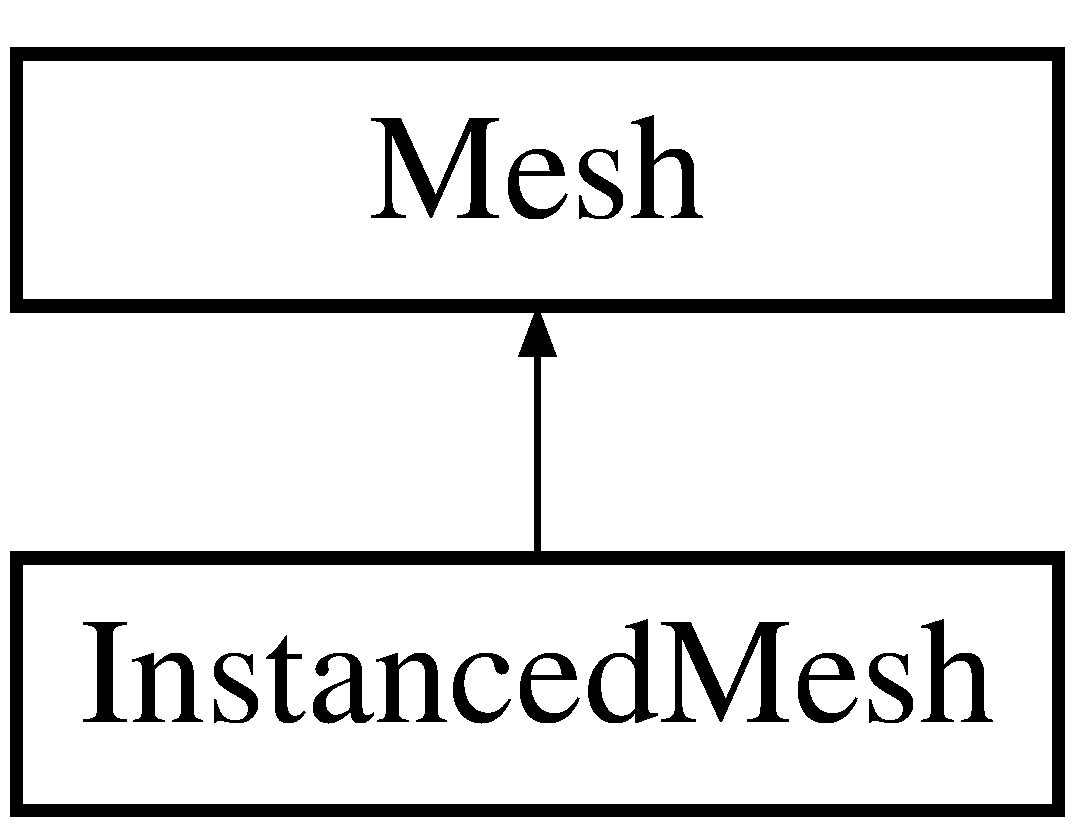
\includegraphics[height=2.000000cm]{class_mesh}
\end{center}
\end{figure}
\subsection*{Public Member Functions}
\begin{DoxyCompactItemize}
\item 
\mbox{\Hypertarget{class_mesh_a921d7db7d2bd9bfd47db709b2bdd6b5c}\label{class_mesh_a921d7db7d2bd9bfd47db709b2bdd6b5c}} 
{\bfseries Mesh} (std\+::string filename)
\item 
\mbox{\Hypertarget{class_mesh_ab432ad94f37ef92e72f13927cc44ecc1}\label{class_mesh_ab432ad94f37ef92e72f13927cc44ecc1}} 
{\bfseries Mesh} (const \mbox{\hyperlink{class_vertex}{Vertex}} $\ast$vertices, std\+::size\+\_\+t number\+\_\+of\+\_\+vertices, const unsigned int $\ast$indices, std\+::size\+\_\+t number\+\_\+of\+\_\+indices)
\item 
\mbox{\Hypertarget{class_mesh_a1bfd1eb4e2530fe0fe46bf798a8b7ecd}\label{class_mesh_a1bfd1eb4e2530fe0fe46bf798a8b7ecd}} 
{\bfseries Mesh} (const std\+::vector$<$ \mbox{\hyperlink{class_vertex}{Vertex}} $>$ \&vertices, const std\+::vector$<$ unsigned int $>$ \&indices)
\item 
\mbox{\Hypertarget{class_mesh_a3687e73537a656b1ada92df6f9930206}\label{class_mesh_a3687e73537a656b1ada92df6f9930206}} 
{\bfseries Mesh} (const \mbox{\hyperlink{class_mesh}{Mesh}} \&copy)=default
\item 
\mbox{\Hypertarget{class_mesh_aa3e0309c79938d016646e14ae4406009}\label{class_mesh_aa3e0309c79938d016646e14ae4406009}} 
{\bfseries Mesh} (\mbox{\hyperlink{class_mesh}{Mesh}} \&\&move)=default
\item 
\mbox{\Hypertarget{class_mesh_aa152c24d58ab422b6d6b24ad9be88a71}\label{class_mesh_aa152c24d58ab422b6d6b24ad9be88a71}} 
\mbox{\hyperlink{class_mesh}{Mesh}} \& {\bfseries operator=} (const \mbox{\hyperlink{class_mesh}{Mesh}} \&rhs)=default
\item 
\mbox{\Hypertarget{class_mesh_afa09e7ec4e4b2b8846c462bc7f9a3a3e}\label{class_mesh_afa09e7ec4e4b2b8846c462bc7f9a3a3e}} 
\mbox{\hyperlink{classtz_1_1graphics_1_1model_1_1_indexed_model}{tz\+::graphics\+::model\+::\+Indexed\+Model}} {\bfseries get\+\_\+indexed\+\_\+model} () const
\item 
\mbox{\Hypertarget{class_mesh_a613ac182bb9f0034dd51ddcbf00988f2}\label{class_mesh_a613ac182bb9f0034dd51ddcbf00988f2}} 
const std\+::vector$<$ \mbox{\hyperlink{class_vector3}{Vector3F}} $>$ \& {\bfseries get\+\_\+positions} () const
\item 
\mbox{\Hypertarget{class_mesh_a902ec7b814fccfb3a15b94606a5fa9df}\label{class_mesh_a902ec7b814fccfb3a15b94606a5fa9df}} 
const std\+::vector$<$ \mbox{\hyperlink{class_vector2}{Vector2F}} $>$ \& {\bfseries get\+\_\+texcoords} () const
\item 
\mbox{\Hypertarget{class_mesh_aa572cef8bcca33c5eb0240be4c83421d}\label{class_mesh_aa572cef8bcca33c5eb0240be4c83421d}} 
const std\+::vector$<$ \mbox{\hyperlink{class_vector3}{Vector3F}} $>$ \& {\bfseries get\+\_\+normals} () const
\item 
\mbox{\Hypertarget{class_mesh_a4fcfee8b20fbd534bfeeb2c67a06c4df}\label{class_mesh_a4fcfee8b20fbd534bfeeb2c67a06c4df}} 
const std\+::vector$<$ \mbox{\hyperlink{class_vector3}{Vector3F}} $>$ \& {\bfseries get\+\_\+tangents} () const
\item 
\mbox{\Hypertarget{class_mesh_ade35393b24319722a76fdfa608e33928}\label{class_mesh_ade35393b24319722a76fdfa608e33928}} 
std\+::string {\bfseries get\+\_\+file\+\_\+name} () const
\item 
\mbox{\Hypertarget{class_mesh_a7efc4ae895a9fac0deda8c5c945c9497}\label{class_mesh_a7efc4ae895a9fac0deda8c5c945c9497}} 
virtual void {\bfseries render} (bool patches, G\+Lenum mode=G\+L\+\_\+\+T\+R\+I\+A\+N\+G\+L\+ES) const
\item 
\mbox{\Hypertarget{class_mesh_a60ab059d5837a5a7bdf4beac14c19b55}\label{class_mesh_a60ab059d5837a5a7bdf4beac14c19b55}} 
bool {\bfseries operator==} (const \mbox{\hyperlink{class_mesh}{Mesh}} \&rhs) const
\end{DoxyCompactItemize}
\subsection*{Protected Attributes}
\begin{DoxyCompactItemize}
\item 
\mbox{\Hypertarget{class_mesh_acd6d79d8a54c6f310cbeccbd5726b942}\label{class_mesh_acd6d79d8a54c6f310cbeccbd5726b942}} 
const std\+::string {\bfseries filename}
\item 
\mbox{\Hypertarget{class_mesh_a9cabf6b1628f877e6c37f55238c01cce}\label{class_mesh_a9cabf6b1628f877e6c37f55238c01cce}} 
\mbox{\hyperlink{classtz_1_1graphics_1_1model_1_1_indexed_model}{tz\+::graphics\+::model\+::\+Indexed\+Model}} {\bfseries model}
\item 
\mbox{\Hypertarget{class_mesh_a5e3901e2d45063e199b701088b28a19c}\label{class_mesh_a5e3901e2d45063e199b701088b28a19c}} 
G\+Luint {\bfseries vertex\+\_\+array\+\_\+object}
\item 
\mbox{\Hypertarget{class_mesh_aded7c34208b8999adf036b587c9aab1a}\label{class_mesh_aded7c34208b8999adf036b587c9aab1a}} 
std\+::array$<$ G\+Luint, static\+\_\+cast$<$ std\+::size\+\_\+t $>$tz\+::graphics\+::\+Buffer\+Types\+::\+N\+U\+M\+\_\+\+B\+U\+F\+F\+E\+RS)$>$ {\bfseries vbo\+\_\+buffers}
\item 
\mbox{\Hypertarget{class_mesh_a426c8e3e3f8b0f11fc0edcf46e39f87b}\label{class_mesh_a426c8e3e3f8b0f11fc0edcf46e39f87b}} 
unsigned int {\bfseries render\+\_\+count}
\end{DoxyCompactItemize}


\subsection{Detailed Description}
Lowest-\/level renderable class that Topaz offers. All renderable Topaz classes such as Object3D contain these. Holds 3D vertex data, from a Wavefront O\+BJ model, for example. Use this if you have an existing shader you can use to draw manually. 

The documentation for this class was generated from the following files\+:\begin{DoxyCompactItemize}
\item 
src/graphics/mesh.\+hpp\item 
src/graphics/mesh.\+cpp\end{DoxyCompactItemize}

\hypertarget{class_mouse_listener}{}\section{Mouse\+Listener Class Reference}
\label{class_mouse_listener}\index{Mouse\+Listener@{Mouse\+Listener}}


{\ttfamily \#include $<$listener.\+hpp$>$}

Inheritance diagram for Mouse\+Listener\+:\begin{figure}[H]
\begin{center}
\leavevmode
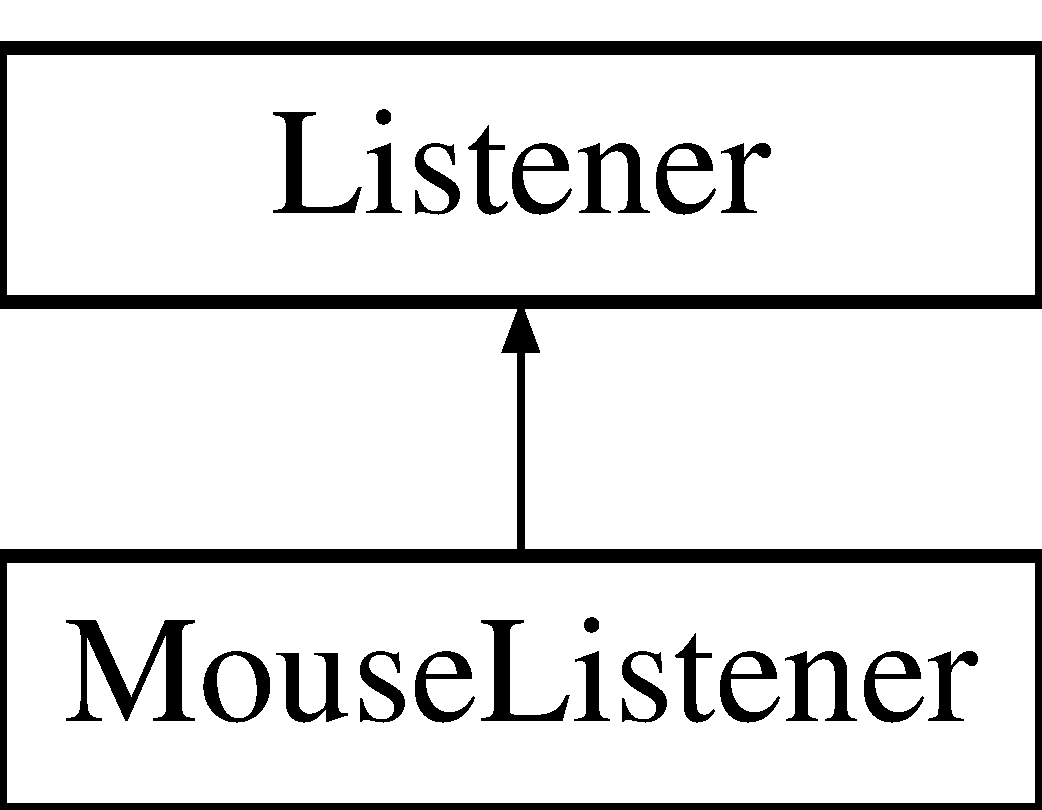
\includegraphics[height=2.000000cm]{class_mouse_listener}
\end{center}
\end{figure}
\subsection*{Public Member Functions}
\begin{DoxyCompactItemize}
\item 
\mbox{\Hypertarget{class_mouse_listener_a7fb712c02cd32dc0f42d1bcc0835fca8}\label{class_mouse_listener_a7fb712c02cd32dc0f42d1bcc0835fca8}} 
{\bfseries Mouse\+Listener} (\mbox{\hyperlink{class_window}{Window}} \&window)
\item 
\mbox{\Hypertarget{class_mouse_listener_ad1c2c314c2efcb7b2f33a214d3ee7ced}\label{class_mouse_listener_ad1c2c314c2efcb7b2f33a214d3ee7ced}} 
{\bfseries Mouse\+Listener} (const \mbox{\hyperlink{class_mouse_listener}{Mouse\+Listener}} \&copy)=default
\item 
\mbox{\Hypertarget{class_mouse_listener_af1b3ec4e87f6843e164a6759ca4d58a8}\label{class_mouse_listener_af1b3ec4e87f6843e164a6759ca4d58a8}} 
{\bfseries Mouse\+Listener} (\mbox{\hyperlink{class_mouse_listener}{Mouse\+Listener}} \&\&move)=default
\item 
\mbox{\Hypertarget{class_mouse_listener_a1846b959ffaab4132f4b22ecd7e8a10e}\label{class_mouse_listener_a1846b959ffaab4132f4b22ecd7e8a10e}} 
\mbox{\hyperlink{class_mouse_listener}{Mouse\+Listener}} \& {\bfseries operator=} (const \mbox{\hyperlink{class_mouse_listener}{Mouse\+Listener}} \&rhs)=default
\item 
\mbox{\Hypertarget{class_mouse_listener_a6ec65116dd06555fbc26ce34bb79e6d4}\label{class_mouse_listener_a6ec65116dd06555fbc26ce34bb79e6d4}} 
virtual void {\bfseries handle\+\_\+events} (S\+D\+L\+\_\+\+Event \&evt) override
\item 
\mbox{\Hypertarget{class_mouse_listener_a9beb1f6d4e96becbba80457977bd5a42}\label{class_mouse_listener_a9beb1f6d4e96becbba80457977bd5a42}} 
void {\bfseries reload\+\_\+mouse\+\_\+delta} ()
\item 
\mbox{\Hypertarget{class_mouse_listener_ad94ea396519a130637e3d5edefa327c2}\label{class_mouse_listener_ad94ea396519a130637e3d5edefa327c2}} 
bool {\bfseries is\+\_\+left\+\_\+clicked} () const
\item 
\mbox{\Hypertarget{class_mouse_listener_aad89212527f27f3b0876a9e7f3c61085}\label{class_mouse_listener_aad89212527f27f3b0876a9e7f3c61085}} 
bool {\bfseries is\+\_\+right\+\_\+clicked} () const
\item 
\mbox{\Hypertarget{class_mouse_listener_a31c56e6e842d815cc5f88fa015d68899}\label{class_mouse_listener_a31c56e6e842d815cc5f88fa015d68899}} 
const \mbox{\hyperlink{class_vector2}{Vector2F}} \& {\bfseries get\+\_\+mouse\+\_\+pos} () const
\item 
\mbox{\Hypertarget{class_mouse_listener_aa10d9b159941d5297fe4e814ad529524}\label{class_mouse_listener_aa10d9b159941d5297fe4e814ad529524}} 
\mbox{\hyperlink{class_vector2}{Vector2F}} {\bfseries get\+\_\+mouse\+\_\+delta\+\_\+pos} () const
\item 
\mbox{\Hypertarget{class_mouse_listener_a1d3c6616b0fe7bdf8f0c31f8cf22ab71}\label{class_mouse_listener_a1d3c6616b0fe7bdf8f0c31f8cf22ab71}} 
const \mbox{\hyperlink{class_vector2}{Vector2F}} \& {\bfseries get\+\_\+left\+\_\+click\+\_\+location} () const
\item 
\mbox{\Hypertarget{class_mouse_listener_a93adff4448210ac95d7aaf870082987d}\label{class_mouse_listener_a93adff4448210ac95d7aaf870082987d}} 
const \mbox{\hyperlink{class_vector2}{Vector2F}} \& {\bfseries get\+\_\+right\+\_\+click\+\_\+location} () const
\end{DoxyCompactItemize}
\subsection*{Additional Inherited Members}


\subsection{Detailed Description}
How Topaz handles mouse input. Register this to a Topaz \mbox{\hyperlink{class_window}{Window}} to use properly. 

The documentation for this class was generated from the following files\+:\begin{DoxyCompactItemize}
\item 
src/listener.\+hpp\item 
src/listener.\+cpp\end{DoxyCompactItemize}

\hypertarget{class_normal_map}{}\section{Normal\+Map Class Reference}
\label{class_normal_map}\index{Normal\+Map@{Normal\+Map}}


{\ttfamily \#include $<$texture.\+hpp$>$}

Inheritance diagram for Normal\+Map\+:\begin{figure}[H]
\begin{center}
\leavevmode
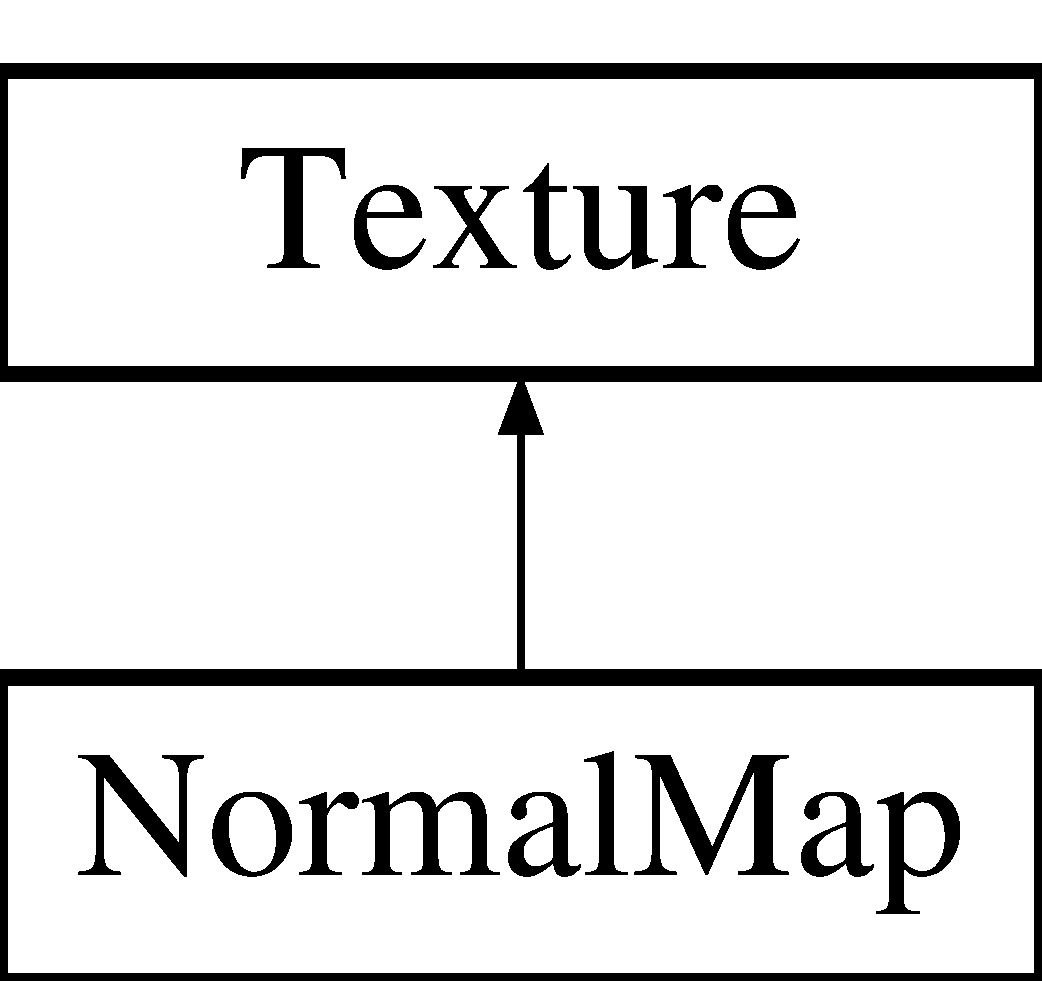
\includegraphics[height=2.000000cm]{class_normal_map}
\end{center}
\end{figure}
\subsection*{Public Member Functions}
\begin{DoxyCompactItemize}
\item 
\mbox{\Hypertarget{class_normal_map_ac654e582d00760ff4043bd9fde77881c}\label{class_normal_map_ac654e582d00760ff4043bd9fde77881c}} 
{\bfseries Normal\+Map} (std\+::string filename)
\item 
\mbox{\Hypertarget{class_normal_map_a9d23a2f3fc54373bc0e3e56940ead720}\label{class_normal_map_a9d23a2f3fc54373bc0e3e56940ead720}} 
virtual void {\bfseries bind} (\mbox{\hyperlink{class_shader}{Shader}} $\ast$shader, unsigned int id) const override
\item 
\mbox{\Hypertarget{class_normal_map_a60bab20997073a76d916b67d520f89a9}\label{class_normal_map_a60bab20997073a76d916b67d520f89a9}} 
virtual tz\+::graphics\+::\+Texture\+Type {\bfseries get\+\_\+texture\+\_\+type} () const override
\end{DoxyCompactItemize}
\subsection*{Additional Inherited Members}


\subsection{Detailed Description}
Representation of a normal-\/map. It\textquotesingle{}s like a texture, but each pixel represents a normal vector for a texel, not colour. 

The documentation for this class was generated from the following file\+:\begin{DoxyCompactItemize}
\item 
src/graphics/texture.\+hpp\end{DoxyCompactItemize}

\hypertarget{class_object}{}\section{Object Class Reference}
\label{class_object}\index{Object@{Object}}


{\ttfamily \#include $<$object.\+hpp$>$}

Inheritance diagram for Object\+:\begin{figure}[H]
\begin{center}
\leavevmode
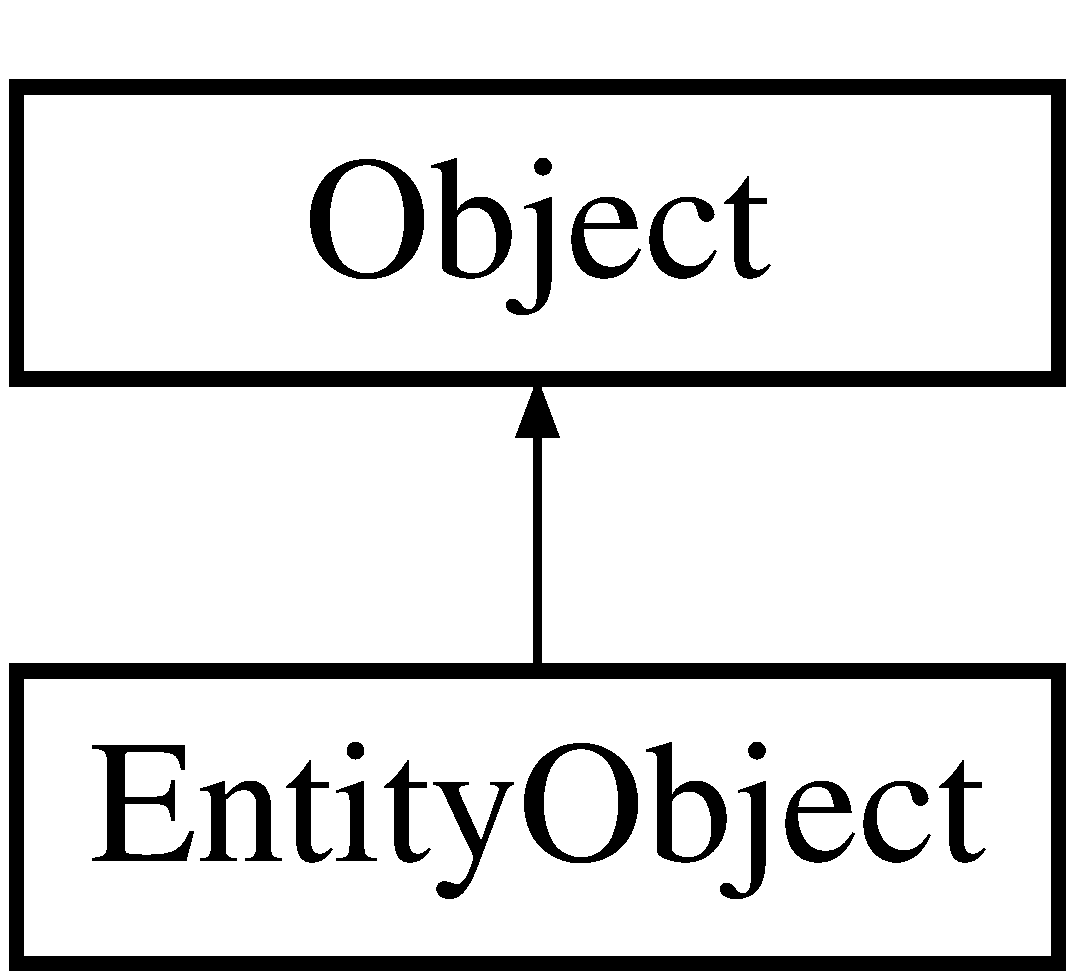
\includegraphics[height=2.000000cm]{class_object}
\end{center}
\end{figure}
\subsection*{Public Member Functions}
\begin{DoxyCompactItemize}
\item 
\mbox{\Hypertarget{class_object_a3852f892594a227653d27b36863b5532}\label{class_object_a3852f892594a227653d27b36863b5532}} 
{\bfseries Object} (std\+::variant$<$ const \mbox{\hyperlink{class_mesh}{Mesh}} $\ast$, std\+::shared\+\_\+ptr$<$ const \mbox{\hyperlink{class_mesh}{Mesh}} $>$$>$ mesh, \mbox{\hyperlink{class_material}{Material}} material, \mbox{\hyperlink{class_vector3}{Vector3F}} position, \mbox{\hyperlink{class_vector3}{Vector3F}} rotation, \mbox{\hyperlink{class_vector3}{Vector3F}} scale)
\item 
\mbox{\Hypertarget{class_object_aaf7dbf04988a46659eca5769c5839e7b}\label{class_object_aaf7dbf04988a46659eca5769c5839e7b}} 
{\bfseries Object} (const \mbox{\hyperlink{class_object}{Object}} \&copy)=default
\item 
\mbox{\Hypertarget{class_object_abc302f6a98cea6288dfee35571485c48}\label{class_object_abc302f6a98cea6288dfee35571485c48}} 
{\bfseries Object} (\mbox{\hyperlink{class_object}{Object}} \&\&move)=default
\item 
\mbox{\Hypertarget{class_object_adc33f671dea9d1e734a2e7991477a004}\label{class_object_adc33f671dea9d1e734a2e7991477a004}} 
\mbox{\hyperlink{class_object}{Object}} \& {\bfseries operator=} (const \mbox{\hyperlink{class_object}{Object}} \&rhs)=default
\item 
\mbox{\Hypertarget{class_object_a7a375f5199dd4508699322a6f18d608d}\label{class_object_a7a375f5199dd4508699322a6f18d608d}} 
const \mbox{\hyperlink{class_mesh}{Mesh}} \& {\bfseries get\+\_\+mesh} () const
\item 
\mbox{\Hypertarget{class_object_a7ed0e8152bdbedc7b289bb6f5d36fa6d}\label{class_object_a7ed0e8152bdbedc7b289bb6f5d36fa6d}} 
const \mbox{\hyperlink{class_material}{Material}} \& {\bfseries get\+\_\+material} () const
\item 
virtual void \mbox{\hyperlink{class_object_adb2402094daa6f7e392c47236d7fef61}{render}} (const \mbox{\hyperlink{class_camera}{Camera}} \&cam, \mbox{\hyperlink{class_shader}{Shader}} $\ast$shader, float width, float height) const
\item 
\mbox{\Hypertarget{class_object_adf4c88351ab218071f5dfc3f111c9a9f}\label{class_object_adf4c88351ab218071f5dfc3f111c9a9f}} 
bool {\bfseries operator==} (const \mbox{\hyperlink{class_object}{Object}} \&rhs) const
\end{DoxyCompactItemize}
\subsection*{Public Attributes}
\begin{DoxyCompactItemize}
\item 
\mbox{\Hypertarget{class_object_a45eaeffd7566fa587d51d47c5c96bdb9}\label{class_object_a45eaeffd7566fa587d51d47c5c96bdb9}} 
\mbox{\hyperlink{class_vector3}{Vector3F}} {\bfseries position}
\item 
\mbox{\Hypertarget{class_object_a753e310c91ea32c22d83a0d241c58cef}\label{class_object_a753e310c91ea32c22d83a0d241c58cef}} 
\mbox{\hyperlink{class_vector3}{Vector3F}} {\bfseries rotation}
\item 
\mbox{\Hypertarget{class_object_a0e8e71418972efbeabe00977dfffa366}\label{class_object_a0e8e71418972efbeabe00977dfffa366}} 
\mbox{\hyperlink{class_vector3}{Vector3F}} {\bfseries scale}
\end{DoxyCompactItemize}
\subsection*{Protected Attributes}
\begin{DoxyCompactItemize}
\item 
\mbox{\Hypertarget{class_object_a4ad1e55e5b3499749f4e78caef74b9c3}\label{class_object_a4ad1e55e5b3499749f4e78caef74b9c3}} 
std\+::variant$<$ const \mbox{\hyperlink{class_mesh}{Mesh}} $\ast$, std\+::shared\+\_\+ptr$<$ const \mbox{\hyperlink{class_mesh}{Mesh}} $>$ $>$ {\bfseries mesh}
\item 
\mbox{\Hypertarget{class_object_a2f63d05a9a9264e1b6c388fa4bba4e91}\label{class_object_a2f63d05a9a9264e1b6c388fa4bba4e91}} 
\mbox{\hyperlink{class_material}{Material}} {\bfseries material}
\end{DoxyCompactItemize}


\subsection{Detailed Description}
Collaboration of a mesh, texture, normal-\/map, parallax-\/map and displacement-\/map Use this to represent a 3D object, including its vertex data, texture, material etc. 

\subsection{Member Function Documentation}
\mbox{\Hypertarget{class_object_adb2402094daa6f7e392c47236d7fef61}\label{class_object_adb2402094daa6f7e392c47236d7fef61}} 
\index{Object@{Object}!render@{render}}
\index{render@{render}!Object@{Object}}
\subsubsection{\texorpdfstring{render()}{render()}}
{\footnotesize\ttfamily void Object\+::render (\begin{DoxyParamCaption}\item[{const \mbox{\hyperlink{class_camera}{Camera}} \&}]{cam,  }\item[{\mbox{\hyperlink{class_shader}{Shader}} $\ast$}]{shader,  }\item[{float}]{width,  }\item[{float}]{height }\end{DoxyParamCaption}) const\hspace{0.3cm}{\ttfamily [virtual]}}

Complexity\+: O(n) Ω(1) ϴ(n), where n =$\sim$ size of mesh data (will not return until G\+PU finishes processing) 

The documentation for this class was generated from the following files\+:\begin{DoxyCompactItemize}
\item 
src/graphics/object.\+hpp\item 
src/graphics/object.\+cpp\end{DoxyCompactItemize}

\hypertarget{class_object2_d}{}\section{Object2D Class Reference}
\label{class_object2_d}\index{Object2D@{Object2D}}


{\ttfamily \#include $<$object.\+hpp$>$}

Inheritance diagram for Object2D\+:\begin{figure}[H]
\begin{center}
\leavevmode
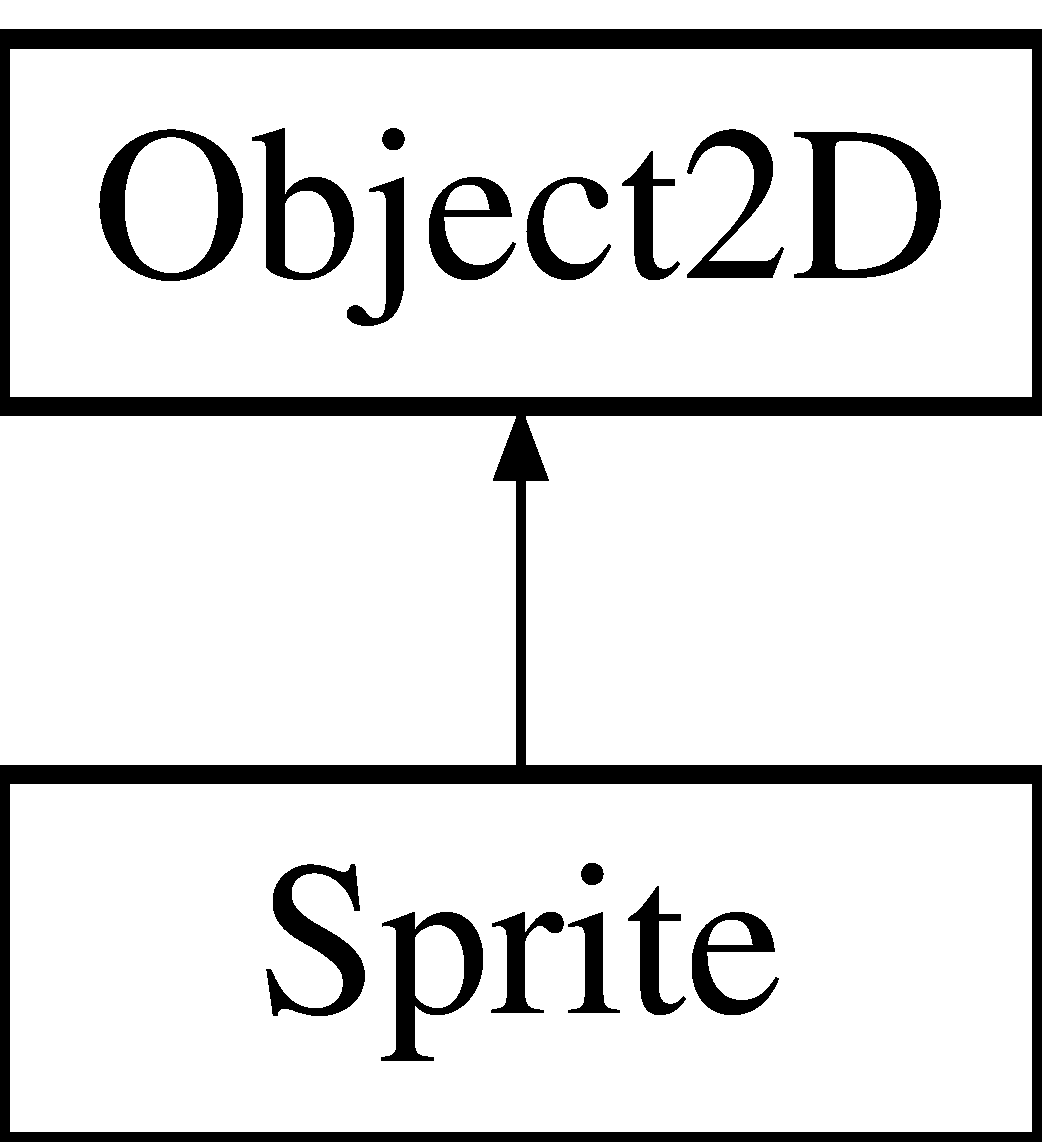
\includegraphics[height=2.000000cm]{class_object2_d}
\end{center}
\end{figure}
\subsection*{Public Member Functions}
\begin{DoxyCompactItemize}
\item 
\mbox{\Hypertarget{class_object2_d_a7d116f8ebc5760f7362e59651d70a6b1}\label{class_object2_d_a7d116f8ebc5760f7362e59651d70a6b1}} 
{\bfseries Object2D} (\mbox{\hyperlink{class_vector2}{Vector2F}} position, float rotation, \mbox{\hyperlink{class_vector2}{Vector2F}} scale, \mbox{\hyperlink{class_vector4}{Vector4F}} colour=\mbox{\hyperlink{class_vector4}{Vector4F}}(0.\+0f, 0.\+0f, 0.\+0f, 1.\+0f))
\item 
\mbox{\Hypertarget{class_object2_d_a2d0b0a3ca540db7062753b858719f288}\label{class_object2_d_a2d0b0a3ca540db7062753b858719f288}} 
\mbox{\hyperlink{class_object2_d}{Object2D}} \& {\bfseries operator=} (const \mbox{\hyperlink{class_object2_d}{Object2D}} \&copy)
\item 
\mbox{\Hypertarget{class_object2_d_a49808683be9af9b5e73da7bc3b37dffd}\label{class_object2_d_a49808683be9af9b5e73da7bc3b37dffd}} 
virtual void {\bfseries render} (const \mbox{\hyperlink{class_camera}{Camera}} \&cam, \mbox{\hyperlink{class_shader}{Shader}} $\ast$shader, float width, float height) const
\end{DoxyCompactItemize}
\subsection*{Public Attributes}
\begin{DoxyCompactItemize}
\item 
\mbox{\Hypertarget{class_object2_d_a93ebae14cceff7ad9aaf0086c7aefb0b}\label{class_object2_d_a93ebae14cceff7ad9aaf0086c7aefb0b}} 
\mbox{\hyperlink{class_vector2}{Vector2F}} {\bfseries position}
\item 
\mbox{\Hypertarget{class_object2_d_adec86c792f1497768570792078c35bc2}\label{class_object2_d_adec86c792f1497768570792078c35bc2}} 
\mbox{\hyperlink{class_vector2}{Vector2F}} {\bfseries scale}
\item 
\mbox{\Hypertarget{class_object2_d_a757b9c0a38f349c8057821dbe2bd14ab}\label{class_object2_d_a757b9c0a38f349c8057821dbe2bd14ab}} 
float {\bfseries rotation}
\item 
\mbox{\Hypertarget{class_object2_d_a27ed9bb852339b71f61a7f79d36dae86}\label{class_object2_d_a27ed9bb852339b71f61a7f79d36dae86}} 
\mbox{\hyperlink{class_vector4}{Vector4F}} {\bfseries colour}
\end{DoxyCompactItemize}
\subsection*{Protected Attributes}
\begin{DoxyCompactItemize}
\item 
\mbox{\Hypertarget{class_object2_d_a7a6d4867eecdb4342b178c9625b4cd67}\label{class_object2_d_a7a6d4867eecdb4342b178c9625b4cd67}} 
\mbox{\hyperlink{class_mesh}{Mesh}} {\bfseries quad}
\end{DoxyCompactItemize}


\subsection{Detailed Description}
Simple plane mesh with a colour to represent a simple-\/sprite. 

The documentation for this class was generated from the following files\+:\begin{DoxyCompactItemize}
\item 
src/graphics/object.\+hpp\item 
src/graphics/object.\+cpp\end{DoxyCompactItemize}

\hypertarget{classtz_1_1graphics_1_1model_1_1_o_b_j_index}{}\section{tz\+:\+:graphics\+:\+:model\+:\+:O\+B\+J\+Index Class Reference}
\label{classtz_1_1graphics_1_1model_1_1_o_b_j_index}\index{tz\+::graphics\+::model\+::\+O\+B\+J\+Index@{tz\+::graphics\+::model\+::\+O\+B\+J\+Index}}
\subsection*{Public Member Functions}
\begin{DoxyCompactItemize}
\item 
\mbox{\Hypertarget{classtz_1_1graphics_1_1model_1_1_o_b_j_index_a5bf098fe36d35780bfb094343361ff83}\label{classtz_1_1graphics_1_1model_1_1_o_b_j_index_a5bf098fe36d35780bfb094343361ff83}} 
bool {\bfseries operator$<$} (const \mbox{\hyperlink{classtz_1_1graphics_1_1model_1_1_o_b_j_index}{O\+B\+J\+Index}} \&rhs) const
\end{DoxyCompactItemize}
\subsection*{Public Attributes}
\begin{DoxyCompactItemize}
\item 
\mbox{\Hypertarget{classtz_1_1graphics_1_1model_1_1_o_b_j_index_a9a846338dd6bad77791041f17545dc01}\label{classtz_1_1graphics_1_1model_1_1_o_b_j_index_a9a846338dd6bad77791041f17545dc01}} 
unsigned int {\bfseries vertex\+\_\+index}
\item 
\mbox{\Hypertarget{classtz_1_1graphics_1_1model_1_1_o_b_j_index_a9b8794bf6a6414055c2ca0b344e23bab}\label{classtz_1_1graphics_1_1model_1_1_o_b_j_index_a9b8794bf6a6414055c2ca0b344e23bab}} 
unsigned int {\bfseries uv\+\_\+index}
\item 
\mbox{\Hypertarget{classtz_1_1graphics_1_1model_1_1_o_b_j_index_a75ae0aff1539b1d346f3114478e6037d}\label{classtz_1_1graphics_1_1model_1_1_o_b_j_index_a75ae0aff1539b1d346f3114478e6037d}} 
unsigned int {\bfseries normal\+\_\+index}
\end{DoxyCompactItemize}


The documentation for this class was generated from the following file\+:\begin{DoxyCompactItemize}
\item 
src/graphics/graphics.\+hpp\end{DoxyCompactItemize}

\hypertarget{classtz_1_1graphics_1_1model_1_1_o_b_j_model}{}\section{tz\+:\+:graphics\+:\+:model\+:\+:O\+B\+J\+Model Class Reference}
\label{classtz_1_1graphics_1_1model_1_1_o_b_j_model}\index{tz\+::graphics\+::model\+::\+O\+B\+J\+Model@{tz\+::graphics\+::model\+::\+O\+B\+J\+Model}}
\subsection*{Public Member Functions}
\begin{DoxyCompactItemize}
\item 
\mbox{\Hypertarget{classtz_1_1graphics_1_1model_1_1_o_b_j_model_a12782990aef3edbf3989dd5115a27c2d}\label{classtz_1_1graphics_1_1model_1_1_o_b_j_model_a12782990aef3edbf3989dd5115a27c2d}} 
{\bfseries O\+B\+J\+Model} (const std\+::string \&file\+\_\+name)
\item 
\mbox{\Hypertarget{classtz_1_1graphics_1_1model_1_1_o_b_j_model_ad0dcb65ddcdf1bb21e74b97235bfa215}\label{classtz_1_1graphics_1_1model_1_1_o_b_j_model_ad0dcb65ddcdf1bb21e74b97235bfa215}} 
\mbox{\hyperlink{classtz_1_1graphics_1_1model_1_1_indexed_model}{Indexed\+Model}} {\bfseries to\+\_\+indexed\+\_\+model} ()
\end{DoxyCompactItemize}
\subsection*{Public Attributes}
\begin{DoxyCompactItemize}
\item 
\mbox{\Hypertarget{classtz_1_1graphics_1_1model_1_1_o_b_j_model_a0f2904907849a9ca1162a60e17d5deb9}\label{classtz_1_1graphics_1_1model_1_1_o_b_j_model_a0f2904907849a9ca1162a60e17d5deb9}} 
std\+::vector$<$ \mbox{\hyperlink{classtz_1_1graphics_1_1model_1_1_o_b_j_index}{O\+B\+J\+Index}} $>$ {\bfseries obj\+\_\+indices}
\item 
\mbox{\Hypertarget{classtz_1_1graphics_1_1model_1_1_o_b_j_model_aec5e5251ce3c0014eea3a39efe4054ea}\label{classtz_1_1graphics_1_1model_1_1_o_b_j_model_aec5e5251ce3c0014eea3a39efe4054ea}} 
std\+::vector$<$ \mbox{\hyperlink{class_vector3}{Vector3F}} $>$ {\bfseries vertices}
\item 
\mbox{\Hypertarget{classtz_1_1graphics_1_1model_1_1_o_b_j_model_a2c07f0f503215dae74a6e7178680d997}\label{classtz_1_1graphics_1_1model_1_1_o_b_j_model_a2c07f0f503215dae74a6e7178680d997}} 
std\+::vector$<$ \mbox{\hyperlink{class_vector2}{Vector2F}} $>$ {\bfseries uvs}
\item 
\mbox{\Hypertarget{classtz_1_1graphics_1_1model_1_1_o_b_j_model_abf68bdb8296b2a8298e591bfbf0075da}\label{classtz_1_1graphics_1_1model_1_1_o_b_j_model_abf68bdb8296b2a8298e591bfbf0075da}} 
std\+::vector$<$ \mbox{\hyperlink{class_vector3}{Vector3F}} $>$ {\bfseries normals}
\item 
\mbox{\Hypertarget{classtz_1_1graphics_1_1model_1_1_o_b_j_model_a0f8dd322a5a87885243cb82d3361d643}\label{classtz_1_1graphics_1_1model_1_1_o_b_j_model_a0f8dd322a5a87885243cb82d3361d643}} 
bool {\bfseries has\+\_\+uvs}
\item 
\mbox{\Hypertarget{classtz_1_1graphics_1_1model_1_1_o_b_j_model_ac5252486a68257bbc480d516d10bf7ba}\label{classtz_1_1graphics_1_1model_1_1_o_b_j_model_ac5252486a68257bbc480d516d10bf7ba}} 
bool {\bfseries has\+\_\+normals}
\end{DoxyCompactItemize}


The documentation for this class was generated from the following files\+:\begin{DoxyCompactItemize}
\item 
src/graphics/graphics.\+hpp\item 
src/graphics/graphics.\+cpp\end{DoxyCompactItemize}

\hypertarget{class_panel}{}\section{Panel Class Reference}
\label{class_panel}\index{Panel@{Panel}}


{\ttfamily \#include $<$gui\+\_\+display.\+hpp$>$}

Inheritance diagram for Panel\+:\begin{figure}[H]
\begin{center}
\leavevmode
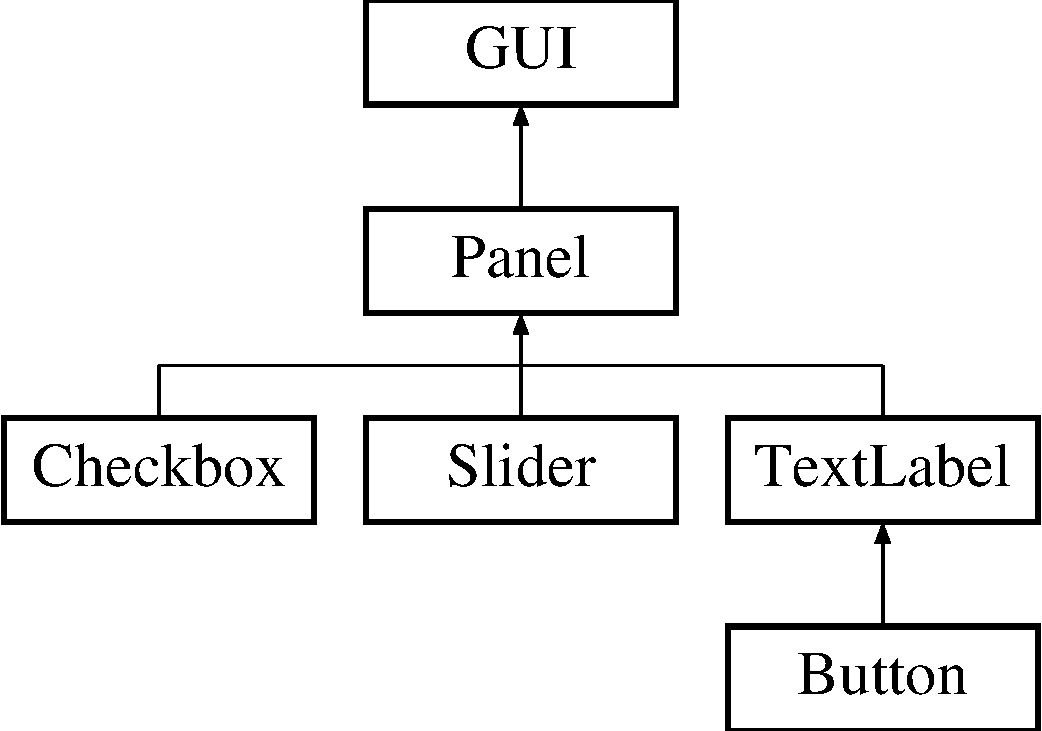
\includegraphics[height=4.000000cm]{class_panel}
\end{center}
\end{figure}
\subsection*{Public Member Functions}
\begin{DoxyCompactItemize}
\item 
\mbox{\hyperlink{class_panel_aafa4aa5f39fb3f832e2f1585ecbce0e9}{Panel}} (float \mbox{\hyperlink{class_g_u_i_a7fa193a8ffb27bbb3bcc225e36f6d54d}{x}}, float \mbox{\hyperlink{class_g_u_i_a98f204f99ffc5ff6cffc9340bbb8c29b}{y}}, float \mbox{\hyperlink{class_g_u_i_aee5d8766834f6f743f0d8b8c16e47155}{width}}, float \mbox{\hyperlink{class_g_u_i_a70b578c36323a45cac88ccff3bced933}{height}}, \mbox{\hyperlink{class_vector4}{Vector4F}} \mbox{\hyperlink{class_panel_a7c38e08ad80eb9972428450fb639bf66}{colour}}, \mbox{\hyperlink{class_shader}{Shader}} \&\mbox{\hyperlink{class_g_u_i_a64b007b31d0ec8a8704f9ab3bb2a7d3d}{shader}})
\item 
const \mbox{\hyperlink{class_vector4}{Vector4F}} \& \mbox{\hyperlink{class_panel_ace1342ef6e7c0f73a44e380356ce5e28}{get\+\_\+colour}} () const
\item 
void \mbox{\hyperlink{class_panel_af23b45cbf03066f1a1d884486ca00712}{set\+\_\+colour}} (\mbox{\hyperlink{class_vector4}{Vector4F}} \mbox{\hyperlink{class_panel_a7c38e08ad80eb9972428450fb639bf66}{colour}})
\item 
const \mbox{\hyperlink{class_texture}{Texture}} $\ast$ \mbox{\hyperlink{class_panel_a938f8a6b4038c5ebd43468ff7c6279c6}{get\+\_\+texture}} () const
\item 
void \mbox{\hyperlink{class_panel_aecd67bfb730ba8e0afd331b5c25c0e83}{set\+\_\+texture}} (\mbox{\hyperlink{class_texture}{Texture}} $\ast$\mbox{\hyperlink{class_panel_a682c2d8747451954095eb567b45d3fbd}{texture}})
\item 
void \mbox{\hyperlink{class_panel_a126b9ac55e35e3530f01614f285e0eea}{disable\+\_\+texture}} ()
\item 
bool \mbox{\hyperlink{class_panel_a3df9165a8d21073e92090937122a790b}{has\+\_\+texture}} () const
\item 
virtual void \mbox{\hyperlink{class_panel_a9e9c0608cf3139833cde6b73dc3ba443}{update}} () override
\item 
virtual void \mbox{\hyperlink{class_panel_ac21884693c47ee069feb9e963f00e9af}{destroy}} () override
\item 
virtual bool \mbox{\hyperlink{class_panel_ace2217419ea5c2e98a38678c6e2012e1}{focused}} () const override
\item 
virtual bool \mbox{\hyperlink{class_panel_a9a30fff40fad1f0845c0c7aa2786f772}{is\+\_\+window}} () const override
\item 
virtual bool \mbox{\hyperlink{class_panel_a607fe6e1be6fd056f199fa817a4dedda}{is\+\_\+mouse\+\_\+sensitive}} () const override
\end{DoxyCompactItemize}
\subsection*{Protected Member Functions}
\begin{DoxyCompactItemize}
\item 
void \mbox{\hyperlink{class_panel_a9f81e58fd5b3d441a145d3aa5e222293}{render\+\_\+panel}} (\mbox{\hyperlink{class_vector4}{Vector4F}} \mbox{\hyperlink{class_panel_a7c38e08ad80eb9972428450fb639bf66}{colour}}, bool \mbox{\hyperlink{class_panel_a9e9c0608cf3139833cde6b73dc3ba443}{update}}=true)
\end{DoxyCompactItemize}
\subsection*{Protected Attributes}
\begin{DoxyCompactItemize}
\item 
\mbox{\Hypertarget{class_panel_a682c2d8747451954095eb567b45d3fbd}\label{class_panel_a682c2d8747451954095eb567b45d3fbd}} 
\mbox{\hyperlink{class_texture}{Texture}} $\ast$ \mbox{\hyperlink{class_panel_a682c2d8747451954095eb567b45d3fbd}{texture}}
\begin{DoxyCompactList}\small\item\em Pointer to the texture which should be displayed on the \mbox{\hyperlink{class_panel}{Panel}} foreground. \end{DoxyCompactList}\item 
\mbox{\Hypertarget{class_panel_a7c38e08ad80eb9972428450fb639bf66}\label{class_panel_a7c38e08ad80eb9972428450fb639bf66}} 
\mbox{\hyperlink{class_vector4}{Vector4F}} \mbox{\hyperlink{class_panel_a7c38e08ad80eb9972428450fb639bf66}{colour}}
\begin{DoxyCompactList}\small\item\em Colour of the \mbox{\hyperlink{class_panel}{Panel}} foreground, if no texture is being displayed. \end{DoxyCompactList}\item 
\mbox{\Hypertarget{class_panel_a3567eff819cd864ee8b6cbce5c01b274}\label{class_panel_a3567eff819cd864ee8b6cbce5c01b274}} 
\mbox{\hyperlink{class_mesh}{Mesh}} \mbox{\hyperlink{class_panel_a3567eff819cd864ee8b6cbce5c01b274}{quad}}
\begin{DoxyCompactList}\small\item\em \mbox{\hyperlink{class_mesh}{Mesh}} representing the quad model of this \mbox{\hyperlink{class_panel}{Panel}}. \end{DoxyCompactList}\end{DoxyCompactItemize}


\subsection{Detailed Description}
A 2D plane rendered on the screen. Can contain any other gui element in its own region. Can have a texture bound, but does not by default. 

\subsection{Constructor \& Destructor Documentation}
\mbox{\Hypertarget{class_panel_aafa4aa5f39fb3f832e2f1585ecbce0e9}\label{class_panel_aafa4aa5f39fb3f832e2f1585ecbce0e9}} 
\index{Panel@{Panel}!Panel@{Panel}}
\index{Panel@{Panel}!Panel@{Panel}}
\subsubsection{\texorpdfstring{Panel()}{Panel()}}
{\footnotesize\ttfamily Panel\+::\+Panel (\begin{DoxyParamCaption}\item[{float}]{x,  }\item[{float}]{y,  }\item[{float}]{width,  }\item[{float}]{height,  }\item[{\mbox{\hyperlink{class_vector4}{Vector4F}}}]{colour,  }\item[{\mbox{\hyperlink{class_shader}{Shader}} \&}]{shader }\end{DoxyParamCaption})}

Construct a \mbox{\hyperlink{class_panel}{Panel}} with all specifications. 
\begin{DoxyParams}{Parameters}
{\em x} & -\/ X-\/coordinate of the \mbox{\hyperlink{class_panel}{Panel}}. \\
\hline
{\em y} & -\/ Y-\/coordinate of the \mbox{\hyperlink{class_panel}{Panel}}. \\
\hline
{\em width} & -\/ Width of the \mbox{\hyperlink{class_panel}{Panel}}. \\
\hline
{\em height} & -\/ Height of the \mbox{\hyperlink{class_panel}{Panel}}. \\
\hline
{\em colour} & -\/ Colour of the \mbox{\hyperlink{class_panel}{Panel}} foreground. \\
\hline
{\em shader} & -\/ The shader with which to render the \mbox{\hyperlink{class_panel}{Panel}}. \\
\hline
\end{DoxyParams}


\subsection{Member Function Documentation}
\mbox{\Hypertarget{class_panel_ac21884693c47ee069feb9e963f00e9af}\label{class_panel_ac21884693c47ee069feb9e963f00e9af}} 
\index{Panel@{Panel}!destroy@{destroy}}
\index{destroy@{destroy}!Panel@{Panel}}
\subsubsection{\texorpdfstring{destroy()}{destroy()}}
{\footnotesize\ttfamily void Panel\+::destroy (\begin{DoxyParamCaption}{ }\end{DoxyParamCaption})\hspace{0.3cm}{\ttfamily [override]}, {\ttfamily [virtual]}}

Destroy the \mbox{\hyperlink{class_panel}{Panel}}, and kill all of its children. 

Reimplemented from \mbox{\hyperlink{class_g_u_i_a2abe7f08a1da35af8ae006fbecea94e0}{G\+UI}}.

\mbox{\Hypertarget{class_panel_a126b9ac55e35e3530f01614f285e0eea}\label{class_panel_a126b9ac55e35e3530f01614f285e0eea}} 
\index{Panel@{Panel}!disable\+\_\+texture@{disable\+\_\+texture}}
\index{disable\+\_\+texture@{disable\+\_\+texture}!Panel@{Panel}}
\subsubsection{\texorpdfstring{disable\+\_\+texture()}{disable\_texture()}}
{\footnotesize\ttfamily void Panel\+::disable\+\_\+texture (\begin{DoxyParamCaption}{ }\end{DoxyParamCaption})}

Stop displaying a texture on this \mbox{\hyperlink{class_panel}{Panel}} and display the foreground-\/colour instead. \mbox{\Hypertarget{class_panel_ace2217419ea5c2e98a38678c6e2012e1}\label{class_panel_ace2217419ea5c2e98a38678c6e2012e1}} 
\index{Panel@{Panel}!focused@{focused}}
\index{focused@{focused}!Panel@{Panel}}
\subsubsection{\texorpdfstring{focused()}{focused()}}
{\footnotesize\ttfamily virtual bool Panel\+::focused (\begin{DoxyParamCaption}{ }\end{DoxyParamCaption}) const\hspace{0.3cm}{\ttfamily [inline]}, {\ttfamily [override]}, {\ttfamily [virtual]}}

Panels cannot be focused. \begin{DoxyReturn}{Returns}
-\/ False 
\end{DoxyReturn}


Implements \mbox{\hyperlink{class_g_u_i_ad2a7c1ae3938ba1d6dea0142f16d6c2b}{G\+UI}}.



Reimplemented in \mbox{\hyperlink{class_slider_a30b01348a5d214f3078e22516c60a763}{Slider}}, \mbox{\hyperlink{class_checkbox_a2a2c82a9e8c95ad868ce85a60ba07292}{Checkbox}}, and \mbox{\hyperlink{class_button_a2c1b0adeb2920b394fe4f38354ae6604}{Button}}.

\mbox{\Hypertarget{class_panel_ace1342ef6e7c0f73a44e380356ce5e28}\label{class_panel_ace1342ef6e7c0f73a44e380356ce5e28}} 
\index{Panel@{Panel}!get\+\_\+colour@{get\+\_\+colour}}
\index{get\+\_\+colour@{get\+\_\+colour}!Panel@{Panel}}
\subsubsection{\texorpdfstring{get\+\_\+colour()}{get\_colour()}}
{\footnotesize\ttfamily const \mbox{\hyperlink{class_vector4}{Vector4F}} \& Panel\+::get\+\_\+colour (\begin{DoxyParamCaption}{ }\end{DoxyParamCaption}) const}

Get the R\+G\+B\+A-\/encoded colour of the \mbox{\hyperlink{class_panel}{Panel}}\textquotesingle{}s foreground. \begin{DoxyReturn}{Returns}
-\/ Colour of the \mbox{\hyperlink{class_panel}{Panel}} foreground 
\end{DoxyReturn}
\mbox{\Hypertarget{class_panel_a938f8a6b4038c5ebd43468ff7c6279c6}\label{class_panel_a938f8a6b4038c5ebd43468ff7c6279c6}} 
\index{Panel@{Panel}!get\+\_\+texture@{get\+\_\+texture}}
\index{get\+\_\+texture@{get\+\_\+texture}!Panel@{Panel}}
\subsubsection{\texorpdfstring{get\+\_\+texture()}{get\_texture()}}
{\footnotesize\ttfamily const \mbox{\hyperlink{class_texture}{Texture}} $\ast$ Panel\+::get\+\_\+texture (\begin{DoxyParamCaption}{ }\end{DoxyParamCaption}) const}

\mbox{\hyperlink{class_texture}{Texture}} pointer that should be displayed on the \mbox{\hyperlink{class_panel}{Panel}}\textquotesingle{}s foreground. \begin{DoxyReturn}{Returns}
-\/ Pointer to the texture used. If no texture is being used, nullptr is returned 
\end{DoxyReturn}
\mbox{\Hypertarget{class_panel_a3df9165a8d21073e92090937122a790b}\label{class_panel_a3df9165a8d21073e92090937122a790b}} 
\index{Panel@{Panel}!has\+\_\+texture@{has\+\_\+texture}}
\index{has\+\_\+texture@{has\+\_\+texture}!Panel@{Panel}}
\subsubsection{\texorpdfstring{has\+\_\+texture()}{has\_texture()}}
{\footnotesize\ttfamily bool Panel\+::has\+\_\+texture (\begin{DoxyParamCaption}{ }\end{DoxyParamCaption}) const}

Query whether this \mbox{\hyperlink{class_panel}{Panel}} is displaying a texture on its foreground. \begin{DoxyReturn}{Returns}
-\/ True if a texture is being displayed. Otherwise false. 
\end{DoxyReturn}
\mbox{\Hypertarget{class_panel_a607fe6e1be6fd056f199fa817a4dedda}\label{class_panel_a607fe6e1be6fd056f199fa817a4dedda}} 
\index{Panel@{Panel}!is\+\_\+mouse\+\_\+sensitive@{is\+\_\+mouse\+\_\+sensitive}}
\index{is\+\_\+mouse\+\_\+sensitive@{is\+\_\+mouse\+\_\+sensitive}!Panel@{Panel}}
\subsubsection{\texorpdfstring{is\+\_\+mouse\+\_\+sensitive()}{is\_mouse\_sensitive()}}
{\footnotesize\ttfamily virtual bool Panel\+::is\+\_\+mouse\+\_\+sensitive (\begin{DoxyParamCaption}{ }\end{DoxyParamCaption}) const\hspace{0.3cm}{\ttfamily [inline]}, {\ttfamily [override]}, {\ttfamily [virtual]}}

Panels are mouse-\/insensitive. \begin{DoxyReturn}{Returns}
-\/ False 
\end{DoxyReturn}


Reimplemented from \mbox{\hyperlink{class_g_u_i_aff34edd65faff6f3e908070a2060f6b8}{G\+UI}}.



Reimplemented in \mbox{\hyperlink{class_slider_a8d7d12aa4bc5d26de46790b43116bcc1}{Slider}}, \mbox{\hyperlink{class_checkbox_a63fc27bae94d81d4dee8cd2d0e474d2b}{Checkbox}}, and \mbox{\hyperlink{class_button_aa2b16ae30fe74f215aa79c699bbf8510}{Button}}.

\mbox{\Hypertarget{class_panel_a9a30fff40fad1f0845c0c7aa2786f772}\label{class_panel_a9a30fff40fad1f0845c0c7aa2786f772}} 
\index{Panel@{Panel}!is\+\_\+window@{is\+\_\+window}}
\index{is\+\_\+window@{is\+\_\+window}!Panel@{Panel}}
\subsubsection{\texorpdfstring{is\+\_\+window()}{is\_window()}}
{\footnotesize\ttfamily virtual bool Panel\+::is\+\_\+window (\begin{DoxyParamCaption}{ }\end{DoxyParamCaption}) const\hspace{0.3cm}{\ttfamily [inline]}, {\ttfamily [override]}, {\ttfamily [virtual]}}

Panels are not Windows. \begin{DoxyReturn}{Returns}
-\/ False 
\end{DoxyReturn}


Implements \mbox{\hyperlink{class_g_u_i_a7ef5287aaa630a8d1146f0d5a35b6683}{G\+UI}}.

\mbox{\Hypertarget{class_panel_a9f81e58fd5b3d441a145d3aa5e222293}\label{class_panel_a9f81e58fd5b3d441a145d3aa5e222293}} 
\index{Panel@{Panel}!render\+\_\+panel@{render\+\_\+panel}}
\index{render\+\_\+panel@{render\+\_\+panel}!Panel@{Panel}}
\subsubsection{\texorpdfstring{render\+\_\+panel()}{render\_panel()}}
{\footnotesize\ttfamily void Panel\+::render\+\_\+panel (\begin{DoxyParamCaption}\item[{\mbox{\hyperlink{class_vector4}{Vector4F}}}]{colour,  }\item[{bool}]{update = {\ttfamily true} }\end{DoxyParamCaption})\hspace{0.3cm}{\ttfamily [protected]}}

Render the \mbox{\hyperlink{class_panel}{Panel}} with the specified colour. 
\begin{DoxyParams}{Parameters}
{\em colour} & -\/ Colour to render the foreground of the \mbox{\hyperlink{class_panel}{Panel}} as. \\
\hline
{\em update} & -\/ Whether to update all the \mbox{\hyperlink{class_panel}{Panel}}\textquotesingle{}s children or not. \\
\hline
\end{DoxyParams}
\mbox{\Hypertarget{class_panel_af23b45cbf03066f1a1d884486ca00712}\label{class_panel_af23b45cbf03066f1a1d884486ca00712}} 
\index{Panel@{Panel}!set\+\_\+colour@{set\+\_\+colour}}
\index{set\+\_\+colour@{set\+\_\+colour}!Panel@{Panel}}
\subsubsection{\texorpdfstring{set\+\_\+colour()}{set\_colour()}}
{\footnotesize\ttfamily void Panel\+::set\+\_\+colour (\begin{DoxyParamCaption}\item[{\mbox{\hyperlink{class_vector4}{Vector4F}}}]{colour }\end{DoxyParamCaption})}

Specify the colour of the \mbox{\hyperlink{class_panel}{Panel}}\textquotesingle{}s foreground. 
\begin{DoxyParams}{Parameters}
{\em colour} & -\/ Desired R\+G\+B\+A-\/encoded colour of the \mbox{\hyperlink{class_panel}{Panel}}\textquotesingle{}s foreground \\
\hline
\end{DoxyParams}
\mbox{\Hypertarget{class_panel_aecd67bfb730ba8e0afd331b5c25c0e83}\label{class_panel_aecd67bfb730ba8e0afd331b5c25c0e83}} 
\index{Panel@{Panel}!set\+\_\+texture@{set\+\_\+texture}}
\index{set\+\_\+texture@{set\+\_\+texture}!Panel@{Panel}}
\subsubsection{\texorpdfstring{set\+\_\+texture()}{set\_texture()}}
{\footnotesize\ttfamily void Panel\+::set\+\_\+texture (\begin{DoxyParamCaption}\item[{\mbox{\hyperlink{class_texture}{Texture}} $\ast$}]{texture }\end{DoxyParamCaption})}

Set which existing texture should be displayed on the \mbox{\hyperlink{class_panel}{Panel}}\textquotesingle{}s foreground. 
\begin{DoxyParams}{Parameters}
{\em texture} & -\/ Pointer to the texture which should be used. If nullptr is specified, no texture will be used and the foreground colour will be used instead \\
\hline
\end{DoxyParams}
\mbox{\Hypertarget{class_panel_a9e9c0608cf3139833cde6b73dc3ba443}\label{class_panel_a9e9c0608cf3139833cde6b73dc3ba443}} 
\index{Panel@{Panel}!update@{update}}
\index{update@{update}!Panel@{Panel}}
\subsubsection{\texorpdfstring{update()}{update()}}
{\footnotesize\ttfamily void Panel\+::update (\begin{DoxyParamCaption}{ }\end{DoxyParamCaption})\hspace{0.3cm}{\ttfamily [override]}, {\ttfamily [virtual]}}

Render the \mbox{\hyperlink{class_panel}{Panel}}, and update all children. 

Reimplemented from \mbox{\hyperlink{class_g_u_i_a947e568bf884a8798e3e368417f662c7}{G\+UI}}.



Reimplemented in \mbox{\hyperlink{class_slider_a4ebd527db54ea263c7d0efe4d1f94e1b}{Slider}}, \mbox{\hyperlink{class_text_label_a350a9edc23e4d2a53374fddc5ddc61cc}{Text\+Label}}, \mbox{\hyperlink{class_checkbox_a69c9fb9ce334fc8ff76c49447f1e002d}{Checkbox}}, and \mbox{\hyperlink{class_button_abda97f1ae8e081da3dbd0b77a27cad9d}{Button}}.



The documentation for this class was generated from the following files\+:\begin{DoxyCompactItemize}
\item 
src/graphics/gui\+\_\+display.\+hpp\item 
src/graphics/gui\+\_\+display.\+cpp\end{DoxyCompactItemize}

\hypertarget{class_parallax_map}{}\section{Parallax\+Map Class Reference}
\label{class_parallax_map}\index{Parallax\+Map@{Parallax\+Map}}
Inheritance diagram for Parallax\+Map\+:\begin{figure}[H]
\begin{center}
\leavevmode
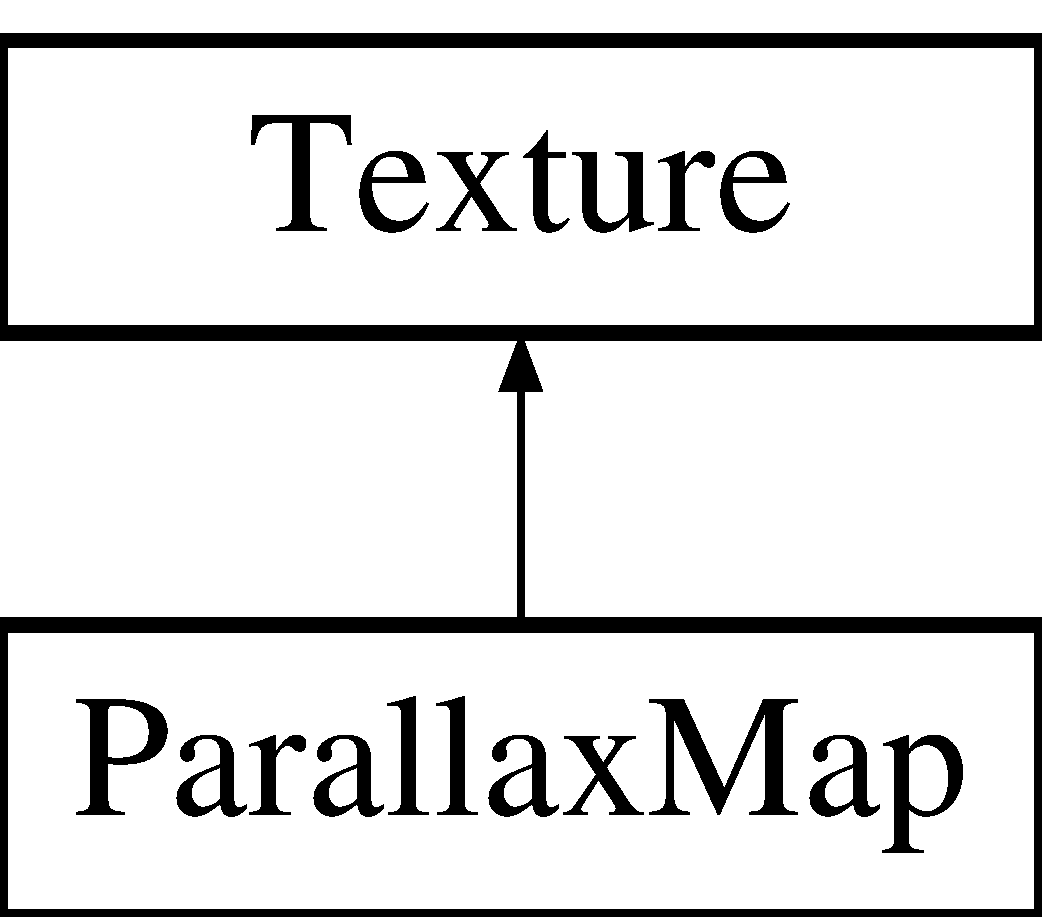
\includegraphics[height=2.000000cm]{class_parallax_map}
\end{center}
\end{figure}
\subsection*{Public Member Functions}
\begin{DoxyCompactItemize}
\item 
\mbox{\Hypertarget{class_parallax_map_a0d7a4d44bf8c5cd8dd920938d6d1e0d2}\label{class_parallax_map_a0d7a4d44bf8c5cd8dd920938d6d1e0d2}} 
{\bfseries Parallax\+Map} (std\+::string filename)
\item 
\mbox{\Hypertarget{class_parallax_map_a2c894a6060a338e9e5c9830bd4c5e93a}\label{class_parallax_map_a2c894a6060a338e9e5c9830bd4c5e93a}} 
virtual void {\bfseries bind} (\mbox{\hyperlink{class_shader}{Shader}} $\ast$shader, unsigned int id) const override
\item 
\mbox{\Hypertarget{class_parallax_map_a56dba3af3087e0f6de74150685881415}\label{class_parallax_map_a56dba3af3087e0f6de74150685881415}} 
virtual tz\+::graphics\+::\+Texture\+Type {\bfseries get\+\_\+texture\+\_\+type} () const override
\end{DoxyCompactItemize}
\subsection*{Additional Inherited Members}


The documentation for this class was generated from the following file\+:\begin{DoxyCompactItemize}
\item 
src/graphics/texture.\+hpp\end{DoxyCompactItemize}

\hypertarget{class_pixel_r_g_b_a}{}\section{Pixel\+R\+G\+BA Class Reference}
\label{class_pixel_r_g_b_a}\index{Pixel\+R\+G\+BA@{Pixel\+R\+G\+BA}}


{\ttfamily \#include $<$graphics.\+hpp$>$}

\subsection*{Public Member Functions}
\begin{DoxyCompactItemize}
\item 
\mbox{\Hypertarget{class_pixel_r_g_b_a_a69b64de852cd399a459b6924e8b3c440}\label{class_pixel_r_g_b_a_a69b64de852cd399a459b6924e8b3c440}} 
constexpr {\bfseries Pixel\+R\+G\+BA} (unsigned char red=0, unsigned char green=0, unsigned char blue=0, unsigned char alpha=0)
\end{DoxyCompactItemize}
\subsection*{Public Attributes}
\begin{DoxyCompactItemize}
\item 
\mbox{\Hypertarget{class_pixel_r_g_b_a_a0a7a223782f5d198363f7ebcf83f4280}\label{class_pixel_r_g_b_a_a0a7a223782f5d198363f7ebcf83f4280}} 
\mbox{\hyperlink{class_vector4}{Vector4}}$<$ unsigned char $>$ {\bfseries data}
\end{DoxyCompactItemize}


\subsection{Detailed Description}
Representation of Pixel Data in R\+G\+BA format. 

The documentation for this class was generated from the following file\+:\begin{DoxyCompactItemize}
\item 
src/graphics/graphics.\+hpp\end{DoxyCompactItemize}

\hypertarget{class_properties_file}{}\section{Properties\+File Class Reference}
\label{class_properties_file}\index{Properties\+File@{Properties\+File}}


{\ttfamily \#include $<$engine\+\_\+meta.\+hpp$>$}

Inheritance diagram for Properties\+File\+:\begin{figure}[H]
\begin{center}
\leavevmode
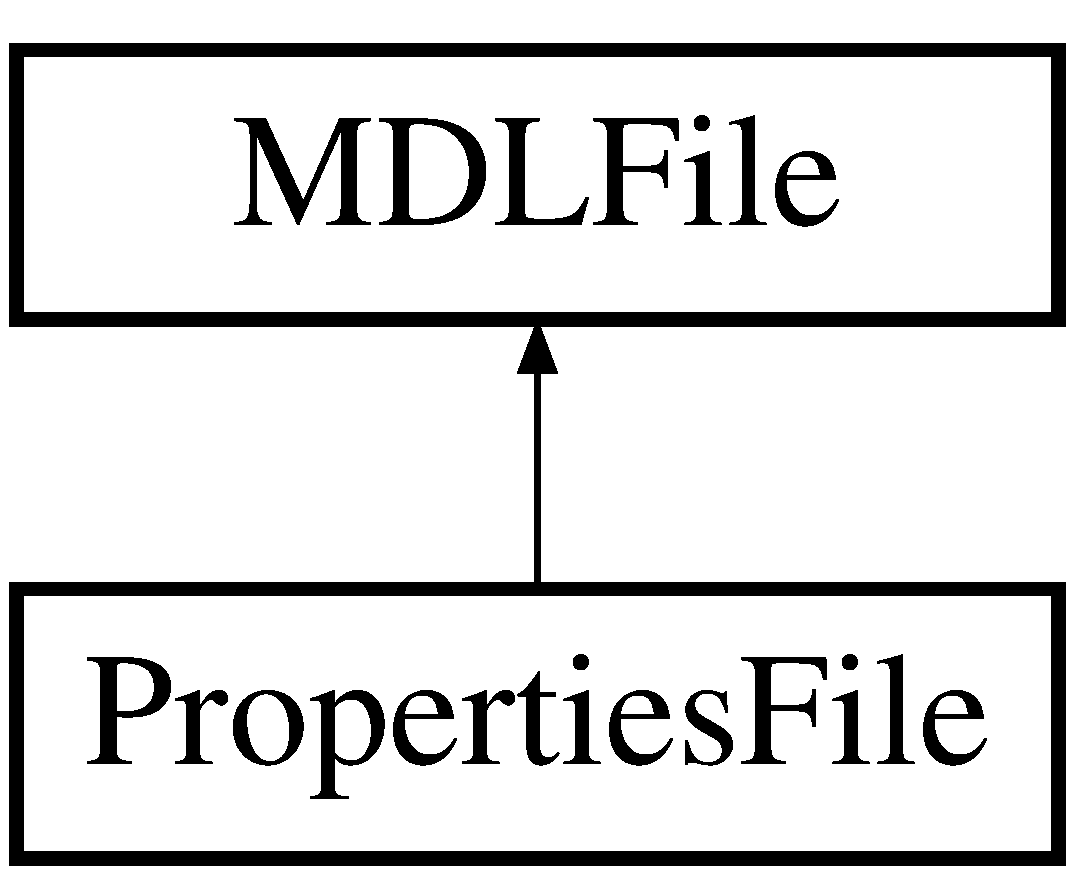
\includegraphics[height=2.000000cm]{class_properties_file}
\end{center}
\end{figure}
\subsection*{Public Member Functions}
\begin{DoxyCompactItemize}
\item 
\mbox{\Hypertarget{class_properties_file_a4e390d378d937c0414402f1b48a9fd39}\label{class_properties_file_a4e390d378d937c0414402f1b48a9fd39}} 
{\bfseries Properties\+File} (std\+::string properties\+\_\+path)
\item 
bool \mbox{\hyperlink{class_properties_file_a9d0632fbdef9f881c065b49d0b4bc7e9}{has\+\_\+inline\+\_\+resources}} () const
\item 
\mbox{\Hypertarget{class_properties_file_aab2a9a8eeaa90367ac6e43d025f684d4}\label{class_properties_file_aab2a9a8eeaa90367ac6e43d025f684d4}} 
std\+::string {\bfseries get\+\_\+property\+\_\+path} (Standard\+Property property) const
\end{DoxyCompactItemize}


\subsection{Detailed Description}
Properties is a file which contains metadata about the Topaz implementation. Specifications such as the default-\/shader, the default-\/gui-\/shader and the Resources location are made here. Properties are normally defined by the filename \textquotesingle{}properties.\+mdl\textquotesingle{} 

\subsection{Member Function Documentation}
\mbox{\Hypertarget{class_properties_file_a9d0632fbdef9f881c065b49d0b4bc7e9}\label{class_properties_file_a9d0632fbdef9f881c065b49d0b4bc7e9}} 
\index{Properties\+File@{Properties\+File}!has\+\_\+inline\+\_\+resources@{has\+\_\+inline\+\_\+resources}}
\index{has\+\_\+inline\+\_\+resources@{has\+\_\+inline\+\_\+resources}!Properties\+File@{Properties\+File}}
\subsubsection{\texorpdfstring{has\+\_\+inline\+\_\+resources()}{has\_inline\_resources()}}
{\footnotesize\ttfamily bool Properties\+File\+::has\+\_\+inline\+\_\+resources (\begin{DoxyParamCaption}{ }\end{DoxyParamCaption}) const}

Returns true if any of the following are true\+:
\begin{DoxyItemize}
\item There is no \textquotesingle{}resources\textquotesingle{} tag
\item The \textquotesingle{}resources\textquotesingle{} tag has a value exactly equal to \textquotesingle{}this\textquotesingle{} \begin{DoxyReturn}{Returns}
-\/ Whether the Properties has inline Resources declared. 
\end{DoxyReturn}

\end{DoxyItemize}

The documentation for this class was generated from the following files\+:\begin{DoxyCompactItemize}
\item 
src/engine\+\_\+meta.\+hpp\item 
src/engine\+\_\+meta.\+cpp\end{DoxyCompactItemize}

\hypertarget{class_quaternion}{}\section{Quaternion Class Reference}
\label{class_quaternion}\index{Quaternion@{Quaternion}}


{\ttfamily \#include $<$quaternion.\+hpp$>$}

Inheritance diagram for Quaternion\+:\begin{figure}[H]
\begin{center}
\leavevmode
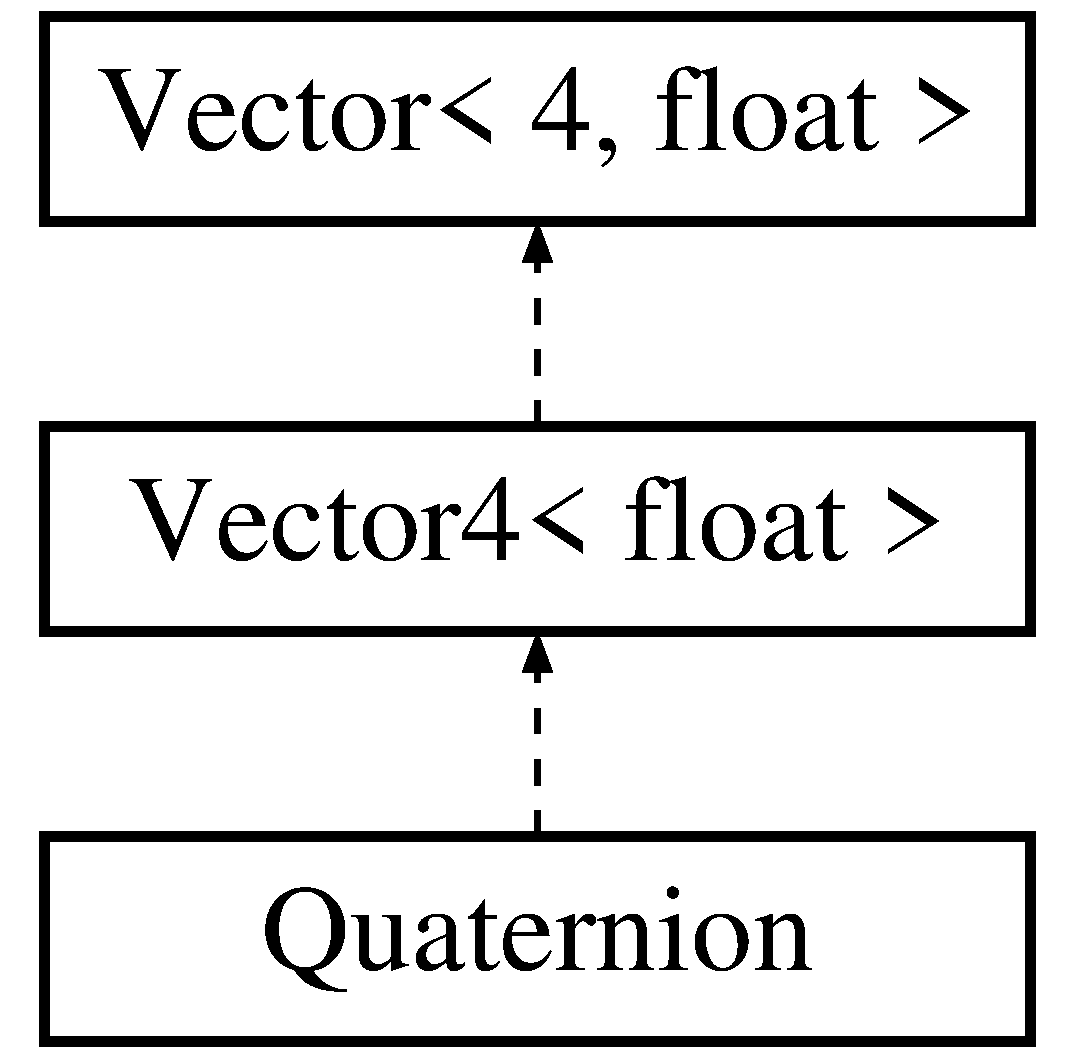
\includegraphics[height=4.000000cm]{class_quaternion}
\end{center}
\end{figure}
\subsection*{Public Member Functions}
\begin{DoxyCompactItemize}
\item 
\mbox{\hyperlink{class_quaternion_a2f9345c4e4ea54370b26cce4d5b075c2}{Quaternion}} (\mbox{\hyperlink{class_vector3}{Vector3F}} rotation\+\_\+axis=\mbox{\hyperlink{class_vector3}{Vector3F}}(), float angle=0.\+0f)
\item 
\mbox{\hyperlink{class_quaternion_a51e4c3b86a987b3c4b3172dac812369f}{Quaternion}} (\mbox{\hyperlink{class_vector3}{Vector3F}} euler\+\_\+rotation)
\item 
\mbox{\hyperlink{class_quaternion_a2d6a1e75c5e91321c0afef7e3ed1b354}{Quaternion}} (\mbox{\hyperlink{class_matrix4x4}{Matrix4x4}} rotational\+\_\+matrix)
\item 
\mbox{\Hypertarget{class_quaternion_aca6deeefa6b6de44aa8e8dd124c6d1ab}\label{class_quaternion_aca6deeefa6b6de44aa8e8dd124c6d1ab}} 
float {\bfseries get\+\_\+angle} () const
\item 
\mbox{\Hypertarget{class_quaternion_ac39a2d53becfbfffe19e374acb33279d}\label{class_quaternion_ac39a2d53becfbfffe19e374acb33279d}} 
\mbox{\hyperlink{class_vector3}{Vector3F}} {\bfseries get\+\_\+rotation\+\_\+axis} () const
\item 
\mbox{\hyperlink{class_matrix4x4}{Matrix4x4}} \mbox{\hyperlink{class_quaternion_ae0309902fc8b7d8aa1f4075a73fee928}{to\+\_\+matrix}} () const
\item 
\mbox{\Hypertarget{class_quaternion_a17008499e6d53e974ee4de8bbbe0cd93}\label{class_quaternion_a17008499e6d53e974ee4de8bbbe0cd93}} 
\mbox{\hyperlink{class_quaternion}{Quaternion}} {\bfseries normalised} () const
\item 
\mbox{\hyperlink{class_quaternion}{Quaternion}} \mbox{\hyperlink{class_quaternion_a38f69dc61e527847ab14b5b6aea5364a}{inverse}} () const
\item 
\mbox{\hyperlink{class_quaternion}{Quaternion}} \mbox{\hyperlink{class_quaternion_aff7a0a5aeea4a3fe860cb90a649e389c}{operator-\/}} () const
\item 
\mbox{\hyperlink{class_matrix4x4}{Matrix4x4}} \mbox{\hyperlink{class_quaternion_afe406f4a387794c924b0459b9514c68d}{operator()}} () const
\item 
\mbox{\hyperlink{class_quaternion_a31f2b4a704b8ba5b677d0cf7ecec163d}{operator Matrix4x4}} () const
\item 
\mbox{\hyperlink{class_quaternion}{Quaternion}} \mbox{\hyperlink{class_quaternion_a7cc9bf508bfd8d521a0d246a2cb47194}{operator$\ast$}} (const \mbox{\hyperlink{class_quaternion}{Quaternion}} \&rhs) const
\item 
\mbox{\Hypertarget{class_quaternion_af19d7a5554539ad967b8c913939dacb6}\label{class_quaternion_af19d7a5554539ad967b8c913939dacb6}} 
\mbox{\hyperlink{class_quaternion}{Quaternion}} {\bfseries operator$\ast$} (float scalar) const
\item 
\mbox{\Hypertarget{class_quaternion_abf1b9fe3ab980e5c97ff0f89c7da9a76}\label{class_quaternion_abf1b9fe3ab980e5c97ff0f89c7da9a76}} 
\mbox{\hyperlink{class_quaternion}{Quaternion}} {\bfseries operator/} (float scalar) const
\item 
\mbox{\hyperlink{class_vector4}{Vector4F}} \mbox{\hyperlink{class_quaternion_af0ec7fb0212b1761149d9bd36bf87455}{operator$\ast$}} (const \mbox{\hyperlink{class_vector3}{Vector3F}} \&vector) const
\end{DoxyCompactItemize}
\subsection*{Additional Inherited Members}


\subsection{Detailed Description}
Represents 3D rotations. Implicitly convertible to a \mbox{\hyperlink{class_matrix4x4}{Matrix4x4}} representing a rotational-\/matrix. 

\subsection{Constructor \& Destructor Documentation}
\mbox{\Hypertarget{class_quaternion_a2f9345c4e4ea54370b26cce4d5b075c2}\label{class_quaternion_a2f9345c4e4ea54370b26cce4d5b075c2}} 
\index{Quaternion@{Quaternion}!Quaternion@{Quaternion}}
\index{Quaternion@{Quaternion}!Quaternion@{Quaternion}}
\subsubsection{\texorpdfstring{Quaternion()}{Quaternion()}\hspace{0.1cm}{\footnotesize\ttfamily [1/3]}}
{\footnotesize\ttfamily Quaternion\+::\+Quaternion (\begin{DoxyParamCaption}\item[{\mbox{\hyperlink{class_vector3}{Vector3F}}}]{rotation\+\_\+axis = {\ttfamily \mbox{\hyperlink{class_vector3}{Vector3F}}()},  }\item[{float}]{angle = {\ttfamily 0.0f} }\end{DoxyParamCaption})}

Construct \mbox{\hyperlink{class_quaternion}{Quaternion}} from a rotation axis and an angle about the axis. \mbox{\Hypertarget{class_quaternion_a51e4c3b86a987b3c4b3172dac812369f}\label{class_quaternion_a51e4c3b86a987b3c4b3172dac812369f}} 
\index{Quaternion@{Quaternion}!Quaternion@{Quaternion}}
\index{Quaternion@{Quaternion}!Quaternion@{Quaternion}}
\subsubsection{\texorpdfstring{Quaternion()}{Quaternion()}\hspace{0.1cm}{\footnotesize\ttfamily [2/3]}}
{\footnotesize\ttfamily Quaternion\+::\+Quaternion (\begin{DoxyParamCaption}\item[{\mbox{\hyperlink{class_vector3}{Vector3F}}}]{euler\+\_\+rotation }\end{DoxyParamCaption})}

Construct \mbox{\hyperlink{class_quaternion}{Quaternion}} from three rotations in euler angles about the three spatial dimensions. \mbox{\Hypertarget{class_quaternion_a2d6a1e75c5e91321c0afef7e3ed1b354}\label{class_quaternion_a2d6a1e75c5e91321c0afef7e3ed1b354}} 
\index{Quaternion@{Quaternion}!Quaternion@{Quaternion}}
\index{Quaternion@{Quaternion}!Quaternion@{Quaternion}}
\subsubsection{\texorpdfstring{Quaternion()}{Quaternion()}\hspace{0.1cm}{\footnotesize\ttfamily [3/3]}}
{\footnotesize\ttfamily Quaternion\+::\+Quaternion (\begin{DoxyParamCaption}\item[{\mbox{\hyperlink{class_matrix4x4}{Matrix4x4}}}]{rotational\+\_\+matrix }\end{DoxyParamCaption})}

Construct \mbox{\hyperlink{class_quaternion}{Quaternion}} from an existing rotational matrix. 

\subsection{Member Function Documentation}
\mbox{\Hypertarget{class_quaternion_a38f69dc61e527847ab14b5b6aea5364a}\label{class_quaternion_a38f69dc61e527847ab14b5b6aea5364a}} 
\index{Quaternion@{Quaternion}!inverse@{inverse}}
\index{inverse@{inverse}!Quaternion@{Quaternion}}
\subsubsection{\texorpdfstring{inverse()}{inverse()}}
{\footnotesize\ttfamily \mbox{\hyperlink{class_quaternion}{Quaternion}} Quaternion\+::inverse (\begin{DoxyParamCaption}{ }\end{DoxyParamCaption}) const}

Just the same as the conjugate of the normalised. \mbox{\Hypertarget{class_quaternion_a31f2b4a704b8ba5b677d0cf7ecec163d}\label{class_quaternion_a31f2b4a704b8ba5b677d0cf7ecec163d}} 
\index{Quaternion@{Quaternion}!operator Matrix4x4@{operator Matrix4x4}}
\index{operator Matrix4x4@{operator Matrix4x4}!Quaternion@{Quaternion}}
\subsubsection{\texorpdfstring{operator Matrix4x4()}{operator Matrix4x4()}}
{\footnotesize\ttfamily Quaternion\+::operator \mbox{\hyperlink{class_matrix4x4}{Matrix4x4}} (\begin{DoxyParamCaption}{ }\end{DoxyParamCaption}) const}

Enable implicit/explicit conversion to the \mbox{\hyperlink{class_matrix4x4}{Matrix4x4}} component (via \mbox{\hyperlink{class_quaternion_ae0309902fc8b7d8aa1f4075a73fee928}{Quaternion\+::to\+\_\+matrix()}}) \mbox{\Hypertarget{class_quaternion_afe406f4a387794c924b0459b9514c68d}\label{class_quaternion_afe406f4a387794c924b0459b9514c68d}} 
\index{Quaternion@{Quaternion}!operator()@{operator()}}
\index{operator()@{operator()}!Quaternion@{Quaternion}}
\subsubsection{\texorpdfstring{operator()()}{operator()()}}
{\footnotesize\ttfamily \mbox{\hyperlink{class_matrix4x4}{Matrix4x4}} Quaternion\+::operator() (\begin{DoxyParamCaption}{ }\end{DoxyParamCaption}) const}

\mbox{\hyperlink{class_quaternion}{Quaternion}} functor returns the Matrix (via \mbox{\hyperlink{class_quaternion_ae0309902fc8b7d8aa1f4075a73fee928}{Quaternion\+::to\+\_\+matrix()}}) \mbox{\Hypertarget{class_quaternion_a7cc9bf508bfd8d521a0d246a2cb47194}\label{class_quaternion_a7cc9bf508bfd8d521a0d246a2cb47194}} 
\index{Quaternion@{Quaternion}!operator$\ast$@{operator$\ast$}}
\index{operator$\ast$@{operator$\ast$}!Quaternion@{Quaternion}}
\subsubsection{\texorpdfstring{operator$\ast$()}{operator*()}\hspace{0.1cm}{\footnotesize\ttfamily [1/2]}}
{\footnotesize\ttfamily \mbox{\hyperlink{class_quaternion}{Quaternion}} Quaternion\+::operator$\ast$ (\begin{DoxyParamCaption}\item[{const \mbox{\hyperlink{class_quaternion}{Quaternion}} \&}]{rhs }\end{DoxyParamCaption}) const}

Combine quaternion rotations. \mbox{\Hypertarget{class_quaternion_af0ec7fb0212b1761149d9bd36bf87455}\label{class_quaternion_af0ec7fb0212b1761149d9bd36bf87455}} 
\index{Quaternion@{Quaternion}!operator$\ast$@{operator$\ast$}}
\index{operator$\ast$@{operator$\ast$}!Quaternion@{Quaternion}}
\subsubsection{\texorpdfstring{operator$\ast$()}{operator*()}\hspace{0.1cm}{\footnotesize\ttfamily [2/2]}}
{\footnotesize\ttfamily \mbox{\hyperlink{class_vector4}{Vector4F}} Quaternion\+::operator$\ast$ (\begin{DoxyParamCaption}\item[{const \mbox{\hyperlink{class_vector3}{Vector3F}} \&}]{vector }\end{DoxyParamCaption}) const}

Rotate a vector by a quaternion. Does not work for homogeneous coordinates; convert to a rotational matrix if you need to do that. \mbox{\Hypertarget{class_quaternion_aff7a0a5aeea4a3fe860cb90a649e389c}\label{class_quaternion_aff7a0a5aeea4a3fe860cb90a649e389c}} 
\index{Quaternion@{Quaternion}!operator-\/@{operator-\/}}
\index{operator-\/@{operator-\/}!Quaternion@{Quaternion}}
\subsubsection{\texorpdfstring{operator-\/()}{operator-()}}
{\footnotesize\ttfamily \mbox{\hyperlink{class_quaternion}{Quaternion}} Quaternion\+::operator-\/ (\begin{DoxyParamCaption}{ }\end{DoxyParamCaption}) const}

Unary operator-\/ is the same as getting the conjugate of the \mbox{\hyperlink{class_quaternion}{Quaternion}} (reversing the polarity A\+KA getting opposite direction of the original rotation axis) \mbox{\Hypertarget{class_quaternion_ae0309902fc8b7d8aa1f4075a73fee928}\label{class_quaternion_ae0309902fc8b7d8aa1f4075a73fee928}} 
\index{Quaternion@{Quaternion}!to\+\_\+matrix@{to\+\_\+matrix}}
\index{to\+\_\+matrix@{to\+\_\+matrix}!Quaternion@{Quaternion}}
\subsubsection{\texorpdfstring{to\+\_\+matrix()}{to\_matrix()}}
{\footnotesize\ttfamily \mbox{\hyperlink{class_matrix4x4}{Matrix4x4}} Quaternion\+::to\+\_\+matrix (\begin{DoxyParamCaption}{ }\end{DoxyParamCaption}) const}

Convert the \mbox{\hyperlink{class_quaternion}{Quaternion}} to a row-\/major rotational matrix. 

The documentation for this class was generated from the following files\+:\begin{DoxyCompactItemize}
\item 
src/quaternion.\+hpp\item 
src/quaternion.\+cpp\end{DoxyCompactItemize}

\hypertarget{class_random}{}\section{Random$<$ Engine, Engine\+Result\+Type $>$ Class Template Reference}
\label{class_random}\index{Random$<$ Engine, Engine\+Result\+Type $>$@{Random$<$ Engine, Engine\+Result\+Type $>$}}


{\ttfamily \#include $<$utility.\+hpp$>$}

\subsection*{Public Member Functions}
\begin{DoxyCompactItemize}
\item 
\mbox{\Hypertarget{class_random_a967417175cc6b2aeee5929f2ea0b178b}\label{class_random_a967417175cc6b2aeee5929f2ea0b178b}} 
{\bfseries Random} (Engine\+Result\+Type seed=std\+::random\+\_\+device()())
\item 
\mbox{\Hypertarget{class_random_abad8ddc1eb952a48a43c0052aa6d280a}\label{class_random_abad8ddc1eb952a48a43c0052aa6d280a}} 
{\bfseries Random} (const \mbox{\hyperlink{class_random}{Random}}$<$ \mbox{\hyperlink{class_engine}{Engine}}, Engine\+Result\+Type $>$ \&copy)
\item 
\mbox{\Hypertarget{class_random_a4381b61f875c2e4746a81fbb967fe667}\label{class_random_a4381b61f875c2e4746a81fbb967fe667}} 
{\bfseries Random} (\mbox{\hyperlink{class_random}{Random}}$<$ \mbox{\hyperlink{class_engine}{Engine}}, Engine\+Result\+Type $>$ \&\&move)=default
\item 
\mbox{\Hypertarget{class_random_a6d2426ffc2369fb7557df8f91a5cf886}\label{class_random_a6d2426ffc2369fb7557df8f91a5cf886}} 
\mbox{\hyperlink{class_random}{Random}}$<$ \mbox{\hyperlink{class_engine}{Engine}}, Engine\+Result\+Type $>$ \& {\bfseries operator=} (const \mbox{\hyperlink{class_random}{Random}}$<$ \mbox{\hyperlink{class_engine}{Engine}}, Engine\+Result\+Type $>$ \&rhs)=default
\item 
\mbox{\Hypertarget{class_random_a1b2ab3fa0602117a6aafa30a7559298c}\label{class_random_a1b2ab3fa0602117a6aafa30a7559298c}} 
const Engine\+Result\+Type \& {\bfseries get\+\_\+seed} () const
\item 
\mbox{\Hypertarget{class_random_a2e7baf19ffba29292bba0f7293d02ec3}\label{class_random_a2e7baf19ffba29292bba0f7293d02ec3}} 
const \mbox{\hyperlink{class_engine}{Engine}} \& {\bfseries get\+\_\+engine} () const
\item 
\mbox{\Hypertarget{class_random_a05a83eaa7ee2e2a73804b6f88efd03f7}\label{class_random_a05a83eaa7ee2e2a73804b6f88efd03f7}} 
int {\bfseries next\+\_\+int} (int min=0, int max=std\+::numeric\+\_\+limits$<$ int $>$\+::max())
\item 
\mbox{\Hypertarget{class_random_ab1e15e656d7750fa1175f4d2e7fcf40c}\label{class_random_ab1e15e656d7750fa1175f4d2e7fcf40c}} 
float {\bfseries next\+\_\+float} (float min=0, float max=std\+::numeric\+\_\+limits$<$ float $>$\+::max())
\item 
\mbox{\Hypertarget{class_random_a33b4d95938e106c260be3464125c43c2}\label{class_random_a33b4d95938e106c260be3464125c43c2}} 
{\footnotesize template$<$typename Number  = int$>$ }\\Number {\bfseries operator()} (Number min=Number(), Number max=std\+::numeric\+\_\+limits$<$ Number $>$\+::max())
\end{DoxyCompactItemize}


\subsection{Detailed Description}
\subsubsection*{template$<$typename Engine = std\+::default\+\_\+random\+\_\+engine, typename Engine\+Result\+Type = std\+::default\+\_\+random\+\_\+engine\+::result\+\_\+type$>$\newline
class Random$<$ Engine, Engine\+Result\+Type $>$}

Generate a random number using any of the C++ standard library random engines. Using default template arguments yields implementation-\/defined behaviour, but normally is a linear-\/congruentional engine. 

The documentation for this class was generated from the following files\+:\begin{DoxyCompactItemize}
\item 
src/utility.\+hpp\item 
src/utility.\+inl\end{DoxyCompactItemize}

\hypertarget{class_render_buffer}{}\section{Render\+Buffer Class Reference}
\label{class_render_buffer}\index{Render\+Buffer@{Render\+Buffer}}


{\ttfamily \#include $<$texture.\+hpp$>$}

\subsection*{Public Member Functions}
\begin{DoxyCompactItemize}
\item 
\mbox{\Hypertarget{class_render_buffer_ad72813870de0738efd5d20ee9b7b221c}\label{class_render_buffer_ad72813870de0738efd5d20ee9b7b221c}} 
{\bfseries Render\+Buffer} (int width, int height, G\+Lenum internal\+\_\+format=G\+L\+\_\+\+R\+G\+BA)
\item 
\mbox{\hyperlink{class_render_buffer_a697b503edabdcc004635382712ea3d22}{Render\+Buffer}} (const \mbox{\hyperlink{class_render_buffer}{Render\+Buffer}} \&copy)=delete
\item 
\mbox{\Hypertarget{class_render_buffer_aba3f5a8b6a083064f9e78eeb1f096d63}\label{class_render_buffer_aba3f5a8b6a083064f9e78eeb1f096d63}} 
{\bfseries Render\+Buffer} (\mbox{\hyperlink{class_render_buffer}{Render\+Buffer}} \&\&move)
\item 
\mbox{\hyperlink{class_render_buffer}{Render\+Buffer}} \& \mbox{\hyperlink{class_render_buffer_a423e4e2601fdda62d63c8fc6a0bb791c}{operator=}} (const \mbox{\hyperlink{class_render_buffer}{Render\+Buffer}} \&rhs)=delete
\end{DoxyCompactItemize}
\subsection*{Friends}
\begin{DoxyCompactItemize}
\item 
\mbox{\Hypertarget{class_render_buffer_a7e815028687ed9f9e9e25851d8a17b27}\label{class_render_buffer_a7e815028687ed9f9e9e25851d8a17b27}} 
class {\bfseries Frame\+Buffer}
\end{DoxyCompactItemize}


\subsection{Detailed Description}
Simple wrapper for an Open\+GL \mbox{\hyperlink{class_render_buffer}{Render\+Buffer}}. It\textquotesingle{}s just a P\+OD as they\textquotesingle{}re write-\/only. 

\subsection{Constructor \& Destructor Documentation}
\mbox{\Hypertarget{class_render_buffer_a697b503edabdcc004635382712ea3d22}\label{class_render_buffer_a697b503edabdcc004635382712ea3d22}} 
\index{Render\+Buffer@{Render\+Buffer}!Render\+Buffer@{Render\+Buffer}}
\index{Render\+Buffer@{Render\+Buffer}!Render\+Buffer@{Render\+Buffer}}
\subsubsection{\texorpdfstring{Render\+Buffer()}{RenderBuffer()}}
{\footnotesize\ttfamily Render\+Buffer\+::\+Render\+Buffer (\begin{DoxyParamCaption}\item[{const \mbox{\hyperlink{class_render_buffer}{Render\+Buffer}} \&}]{copy }\end{DoxyParamCaption})\hspace{0.3cm}{\ttfamily [delete]}}

Open\+GL Render\+Buffers are write-\/only, so cannot possibly read the data in which to copy or move. 

\subsection{Member Function Documentation}
\mbox{\Hypertarget{class_render_buffer_a423e4e2601fdda62d63c8fc6a0bb791c}\label{class_render_buffer_a423e4e2601fdda62d63c8fc6a0bb791c}} 
\index{Render\+Buffer@{Render\+Buffer}!operator=@{operator=}}
\index{operator=@{operator=}!Render\+Buffer@{Render\+Buffer}}
\subsubsection{\texorpdfstring{operator=()}{operator=()}}
{\footnotesize\ttfamily \mbox{\hyperlink{class_render_buffer}{Render\+Buffer}}\& Render\+Buffer\+::operator= (\begin{DoxyParamCaption}\item[{const \mbox{\hyperlink{class_render_buffer}{Render\+Buffer}} \&}]{rhs }\end{DoxyParamCaption})\hspace{0.3cm}{\ttfamily [delete]}}

\mbox{\hyperlink{class_render_buffer_a423e4e2601fdda62d63c8fc6a0bb791c}{Render\+Buffer\+::operator=}} shall act like a pointer-\/copy; both share the same handle. However, when one dies the other becomes invalid, so this will be deleted too. 

The documentation for this class was generated from the following files\+:\begin{DoxyCompactItemize}
\item 
src/graphics/texture.\+hpp\item 
src/graphics/texture.\+cpp\end{DoxyCompactItemize}

\hypertarget{class_resources_file}{}\section{Resources\+File Class Reference}
\label{class_resources_file}\index{Resources\+File@{Resources\+File}}
Inheritance diagram for Resources\+File\+:\begin{figure}[H]
\begin{center}
\leavevmode
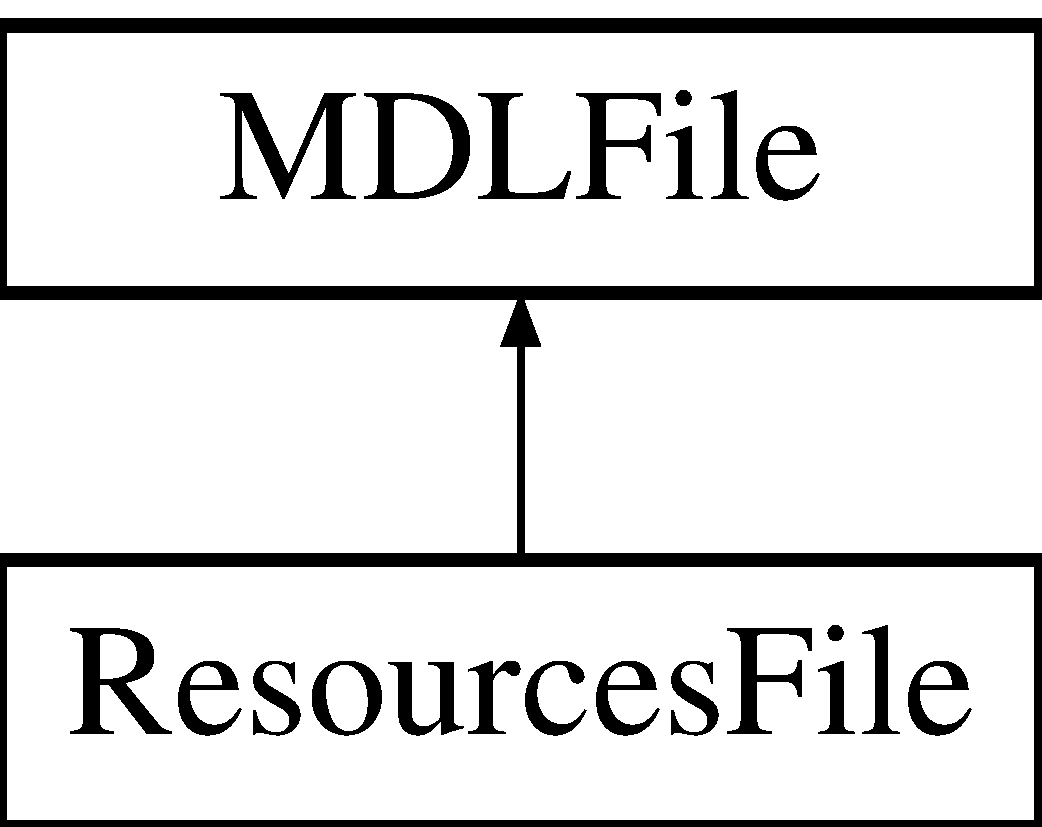
\includegraphics[height=2.000000cm]{class_resources_file}
\end{center}
\end{figure}
\subsection*{Public Member Functions}
\begin{DoxyCompactItemize}
\item 
\mbox{\Hypertarget{class_resources_file_af54641444509becb743c53c807229ccb}\label{class_resources_file_af54641444509becb743c53c807229ccb}} 
{\bfseries Resources\+File} (std\+::string resources\+\_\+path)
\end{DoxyCompactItemize}


The documentation for this class was generated from the following files\+:\begin{DoxyCompactItemize}
\item 
src/engine\+\_\+meta.\+hpp\item 
src/engine\+\_\+meta.\+cpp\end{DoxyCompactItemize}

\hypertarget{class_scene}{}\section{Scene Class Reference}
\label{class_scene}\index{Scene@{Scene}}


{\ttfamily \#include $<$scene.\+hpp$>$}

\subsection*{Public Member Functions}
\begin{DoxyCompactItemize}
\item 
\mbox{\hyperlink{class_scene_ad10176d75a9cc0da56626f682d083507}{Scene}} ()
\item 
\mbox{\hyperlink{class_scene_a5311ceba0e507f805d3c5592155880fc}{Scene}} (std\+::string filename, std\+::string resources\+\_\+path, const std\+::vector$<$ std\+::unique\+\_\+ptr$<$ \mbox{\hyperlink{class_mesh}{Mesh}} $>$$>$ \&all\+\_\+meshes, const std\+::vector$<$ std\+::unique\+\_\+ptr$<$ \mbox{\hyperlink{class_texture}{Texture}} $>$$>$ \&all\+\_\+textures, const std\+::vector$<$ std\+::unique\+\_\+ptr$<$ \mbox{\hyperlink{class_normal_map}{Normal\+Map}} $>$$>$ \&all\+\_\+normal\+\_\+maps, const std\+::vector$<$ std\+::unique\+\_\+ptr$<$ \mbox{\hyperlink{class_parallax_map}{Parallax\+Map}} $>$$>$ \&all\+\_\+parallax\+\_\+maps, const std\+::vector$<$ std\+::unique\+\_\+ptr$<$ \mbox{\hyperlink{class_displacement_map}{Displacement\+Map}} $>$$>$ \&all\+\_\+displacement\+\_\+maps, bool batch=true)
\item 
\mbox{\Hypertarget{class_scene_a04c85384325f658ca37be623fcffd941}\label{class_scene_a04c85384325f658ca37be623fcffd941}} 
{\bfseries Scene} (const \mbox{\hyperlink{class_scene}{Scene}} \&copy)=default
\item 
\mbox{\Hypertarget{class_scene_ac5227706d25b78969a6e37956fc49ebe}\label{class_scene_ac5227706d25b78969a6e37956fc49ebe}} 
{\bfseries Scene} (\mbox{\hyperlink{class_scene}{Scene}} \&\&move)=default
\item 
\mbox{\Hypertarget{class_scene_accf9a458cf5352398186960f362930d0}\label{class_scene_accf9a458cf5352398186960f362930d0}} 
\mbox{\hyperlink{class_scene}{Scene}} \& {\bfseries operator=} (const \mbox{\hyperlink{class_scene}{Scene}} \&rhs)=default
\item 
bool \mbox{\hyperlink{class_scene_a743728388c669fc24f8bd3630f785fbe}{has\+\_\+file\+\_\+name}} () const
\item 
const std\+::string \& \mbox{\hyperlink{class_scene_ad421371655da7444220b21ba150ee3ce}{get\+\_\+file\+\_\+name}} () const
\item 
void \mbox{\hyperlink{class_scene_a6af6561348957b6ce78e851390bc2d58}{add\+\_\+object}} (\mbox{\hyperlink{class_object}{Object}} obj)
\item 
{\footnotesize template$<$class Element , typename... Args$>$ }\\Element \& \mbox{\hyperlink{class_scene_ab49d36bd44583a0374eedf41ccce75d3}{emplace}} (Args \&\&... args)
\item 
{\footnotesize template$<$typename... Args$>$ }\\\mbox{\hyperlink{class_object}{Object}} \& \mbox{\hyperlink{class_scene_a5875b3cf7be811378d53f0fba76cb181}{emplace\+\_\+object}} (Args \&\&... args)
\item 
void \mbox{\hyperlink{class_scene_ad73b372380c1dece59733bf31e38eb19}{remove\+\_\+object}} (const \mbox{\hyperlink{class_object}{Object}} \&obj)
\item 
std\+::vector$<$ std\+::reference\+\_\+wrapper$<$ const \mbox{\hyperlink{class_object}{Object}} $>$ $>$ \mbox{\hyperlink{class_scene_aeac49e2c0a9d551af5419e05f449842c}{get\+\_\+objects}} () const
\item 
std\+::size\+\_\+t \mbox{\hyperlink{class_scene_afb4f9eb929eef70ad8580a00797442a4}{get\+\_\+size}} () const
\item 
void \mbox{\hyperlink{class_scene_a65b10c0a127b5f811869a605b70c5a72}{export\+\_\+scene}} (const std\+::string \&scene\+\_\+link) const
\item 
void \mbox{\hyperlink{class_scene_a6063cdee2eaaf56fd8bf91ba961007f4}{save}} () const
\item 
void \mbox{\hyperlink{class_scene_a6e27640f9973c00e12cf6736bd3c01ad}{render}} (const \mbox{\hyperlink{class_camera}{Camera}} \&cam, \mbox{\hyperlink{class_shader}{Shader}} $\ast$shader, unsigned int width, unsigned int height)
\end{DoxyCompactItemize}
\subsection*{Public Attributes}
\begin{DoxyCompactItemize}
\item 
\mbox{\Hypertarget{class_scene_aa8f56e40ee0ad8f9cedf6e0983b9e328}\label{class_scene_aa8f56e40ee0ad8f9cedf6e0983b9e328}} 
\mbox{\hyperlink{class_vector3}{Vector3F}} {\bfseries spawn\+\_\+point}
\item 
\mbox{\Hypertarget{class_scene_a22378f8dba2c75bd8451c2ecdcab3bd7}\label{class_scene_a22378f8dba2c75bd8451c2ecdcab3bd7}} 
\mbox{\hyperlink{class_vector3}{Vector3F}} {\bfseries spawn\+\_\+orientation}
\end{DoxyCompactItemize}


\subsection{Detailed Description}
Contains Objects, Entity\+Objects and pretty much any Topaz renderable you can think of. Use Scenes to store everything you want to draw. 

\subsection{Constructor \& Destructor Documentation}
\mbox{\Hypertarget{class_scene_ad10176d75a9cc0da56626f682d083507}\label{class_scene_ad10176d75a9cc0da56626f682d083507}} 
\index{Scene@{Scene}!Scene@{Scene}}
\index{Scene@{Scene}!Scene@{Scene}}
\subsubsection{\texorpdfstring{Scene()}{Scene()}\hspace{0.1cm}{\footnotesize\ttfamily [1/2]}}
{\footnotesize\ttfamily Scene\+::\+Scene (\begin{DoxyParamCaption}{ }\end{DoxyParamCaption})}

Construct an empty scene. \mbox{\Hypertarget{class_scene_a5311ceba0e507f805d3c5592155880fc}\label{class_scene_a5311ceba0e507f805d3c5592155880fc}} 
\index{Scene@{Scene}!Scene@{Scene}}
\index{Scene@{Scene}!Scene@{Scene}}
\subsubsection{\texorpdfstring{Scene()}{Scene()}\hspace{0.1cm}{\footnotesize\ttfamily [2/2]}}
{\footnotesize\ttfamily Scene\+::\+Scene (\begin{DoxyParamCaption}\item[{std\+::string}]{filename,  }\item[{std\+::string}]{resources\+\_\+path,  }\item[{const std\+::vector$<$ std\+::unique\+\_\+ptr$<$ \mbox{\hyperlink{class_mesh}{Mesh}} $>$$>$ \&}]{all\+\_\+meshes,  }\item[{const std\+::vector$<$ std\+::unique\+\_\+ptr$<$ \mbox{\hyperlink{class_texture}{Texture}} $>$$>$ \&}]{all\+\_\+textures,  }\item[{const std\+::vector$<$ std\+::unique\+\_\+ptr$<$ \mbox{\hyperlink{class_normal_map}{Normal\+Map}} $>$$>$ \&}]{all\+\_\+normal\+\_\+maps,  }\item[{const std\+::vector$<$ std\+::unique\+\_\+ptr$<$ \mbox{\hyperlink{class_parallax_map}{Parallax\+Map}} $>$$>$ \&}]{all\+\_\+parallax\+\_\+maps,  }\item[{const std\+::vector$<$ std\+::unique\+\_\+ptr$<$ \mbox{\hyperlink{class_displacement_map}{Displacement\+Map}} $>$$>$ \&}]{all\+\_\+displacement\+\_\+maps,  }\item[{bool}]{batch = {\ttfamily true} }\end{DoxyParamCaption})}

Load a scene from an existing M\+DL file. Takes in all asset vectors. Should probably be replaced with just a const asset manager reference of some kind to read the data without all this verbosity. 

\subsection{Member Function Documentation}
\mbox{\Hypertarget{class_scene_a6af6561348957b6ce78e851390bc2d58}\label{class_scene_a6af6561348957b6ce78e851390bc2d58}} 
\index{Scene@{Scene}!add\+\_\+object@{add\+\_\+object}}
\index{add\+\_\+object@{add\+\_\+object}!Scene@{Scene}}
\subsubsection{\texorpdfstring{add\+\_\+object()}{add\_object()}}
{\footnotesize\ttfamily void Scene\+::add\+\_\+object (\begin{DoxyParamCaption}\item[{\mbox{\hyperlink{class_object}{Object}}}]{obj }\end{DoxyParamCaption})}

Add a copy of an object to the scene. Complexity\+: O(1) amortised Ω(1) amortised ϴ(1) amortised. \mbox{\Hypertarget{class_scene_ab49d36bd44583a0374eedf41ccce75d3}\label{class_scene_ab49d36bd44583a0374eedf41ccce75d3}} 
\index{Scene@{Scene}!emplace@{emplace}}
\index{emplace@{emplace}!Scene@{Scene}}
\subsubsection{\texorpdfstring{emplace()}{emplace()}}
{\footnotesize\ttfamily template$<$class Element , typename... Args$>$ \\
Element \& Scene\+::emplace (\begin{DoxyParamCaption}\item[{Args \&\&...}]{args }\end{DoxyParamCaption})}

Construct an \mbox{\hyperlink{class_object}{Object}} or any subclass of \mbox{\hyperlink{class_object}{Object}} in-\/place and add it to the scene. Complexity\+: O(1) amortised Ω(1) amortised ϴ(1) amortised. Element is inherited from \mbox{\hyperlink{class_object}{Object}} so should be emplaced via heap \mbox{\Hypertarget{class_scene_a5875b3cf7be811378d53f0fba76cb181}\label{class_scene_a5875b3cf7be811378d53f0fba76cb181}} 
\index{Scene@{Scene}!emplace\+\_\+object@{emplace\+\_\+object}}
\index{emplace\+\_\+object@{emplace\+\_\+object}!Scene@{Scene}}
\subsubsection{\texorpdfstring{emplace\+\_\+object()}{emplace\_object()}}
{\footnotesize\ttfamily template$<$typename... Args$>$ \\
\mbox{\hyperlink{class_object}{Object}} \& Scene\+::emplace\+\_\+object (\begin{DoxyParamCaption}\item[{Args \&\&...}]{args }\end{DoxyParamCaption})}

Construct an \mbox{\hyperlink{class_object}{Object}} in-\/place and add it to the scene. Object-\/slicing will affect the parameter. Use \mbox{\hyperlink{class_scene_ab49d36bd44583a0374eedf41ccce75d3}{Scene\+::emplace}} instead to prevent slicing. Complexity\+: O(1) amortised Ω(1) amortised ϴ(1) amortised. \mbox{\Hypertarget{class_scene_a65b10c0a127b5f811869a605b70c5a72}\label{class_scene_a65b10c0a127b5f811869a605b70c5a72}} 
\index{Scene@{Scene}!export\+\_\+scene@{export\+\_\+scene}}
\index{export\+\_\+scene@{export\+\_\+scene}!Scene@{Scene}}
\subsubsection{\texorpdfstring{export\+\_\+scene()}{export\_scene()}}
{\footnotesize\ttfamily void Scene\+::export\+\_\+scene (\begin{DoxyParamCaption}\item[{const std\+::string \&}]{scene\+\_\+link }\end{DoxyParamCaption}) const}

Export scene data to a M\+DL file called scene\+\_\+link Complexity\+: O(n + m) Ω(1) ϴ(n + m), where n = number of objects and m = number of entity\+\_\+objects. \mbox{\Hypertarget{class_scene_ad421371655da7444220b21ba150ee3ce}\label{class_scene_ad421371655da7444220b21ba150ee3ce}} 
\index{Scene@{Scene}!get\+\_\+file\+\_\+name@{get\+\_\+file\+\_\+name}}
\index{get\+\_\+file\+\_\+name@{get\+\_\+file\+\_\+name}!Scene@{Scene}}
\subsubsection{\texorpdfstring{get\+\_\+file\+\_\+name()}{get\_file\_name()}}
{\footnotesize\ttfamily const std\+::string \& Scene\+::get\+\_\+file\+\_\+name (\begin{DoxyParamCaption}{ }\end{DoxyParamCaption}) const}

Throws a std\+::bad\+\_\+optional\+\_\+access exception if this-\/$>$\mbox{\hyperlink{class_scene_a743728388c669fc24f8bd3630f785fbe}{has\+\_\+file\+\_\+name()}} returns false. \mbox{\Hypertarget{class_scene_aeac49e2c0a9d551af5419e05f449842c}\label{class_scene_aeac49e2c0a9d551af5419e05f449842c}} 
\index{Scene@{Scene}!get\+\_\+objects@{get\+\_\+objects}}
\index{get\+\_\+objects@{get\+\_\+objects}!Scene@{Scene}}
\subsubsection{\texorpdfstring{get\+\_\+objects()}{get\_objects()}}
{\footnotesize\ttfamily std\+::vector$<$ std\+::reference\+\_\+wrapper$<$ const \mbox{\hyperlink{class_object}{Object}} $>$ $>$ Scene\+::get\+\_\+objects (\begin{DoxyParamCaption}{ }\end{DoxyParamCaption}) const}

Access all \mbox{\hyperlink{class_object}{Object}} elements in the scene (Read-\/only). \mbox{\Hypertarget{class_scene_afb4f9eb929eef70ad8580a00797442a4}\label{class_scene_afb4f9eb929eef70ad8580a00797442a4}} 
\index{Scene@{Scene}!get\+\_\+size@{get\+\_\+size}}
\index{get\+\_\+size@{get\+\_\+size}!Scene@{Scene}}
\subsubsection{\texorpdfstring{get\+\_\+size()}{get\_size()}}
{\footnotesize\ttfamily std\+::size\+\_\+t Scene\+::get\+\_\+size (\begin{DoxyParamCaption}{ }\end{DoxyParamCaption}) const}

Returns total number of Objects in the scene. \mbox{\Hypertarget{class_scene_a743728388c669fc24f8bd3630f785fbe}\label{class_scene_a743728388c669fc24f8bd3630f785fbe}} 
\index{Scene@{Scene}!has\+\_\+file\+\_\+name@{has\+\_\+file\+\_\+name}}
\index{has\+\_\+file\+\_\+name@{has\+\_\+file\+\_\+name}!Scene@{Scene}}
\subsubsection{\texorpdfstring{has\+\_\+file\+\_\+name()}{has\_file\_name()}}
{\footnotesize\ttfamily bool Scene\+::has\+\_\+file\+\_\+name (\begin{DoxyParamCaption}{ }\end{DoxyParamCaption}) const}

Returns true if the scene was loaded from an external file. \mbox{\Hypertarget{class_scene_ad73b372380c1dece59733bf31e38eb19}\label{class_scene_ad73b372380c1dece59733bf31e38eb19}} 
\index{Scene@{Scene}!remove\+\_\+object@{remove\+\_\+object}}
\index{remove\+\_\+object@{remove\+\_\+object}!Scene@{Scene}}
\subsubsection{\texorpdfstring{remove\+\_\+object()}{remove\_object()}}
{\footnotesize\ttfamily void Scene\+::remove\+\_\+object (\begin{DoxyParamCaption}\item[{const \mbox{\hyperlink{class_object}{Object}} \&}]{obj }\end{DoxyParamCaption})}

Remove an existing \mbox{\hyperlink{class_object}{Object}} from the scene. \mbox{\Hypertarget{class_scene_a6e27640f9973c00e12cf6736bd3c01ad}\label{class_scene_a6e27640f9973c00e12cf6736bd3c01ad}} 
\index{Scene@{Scene}!render@{render}}
\index{render@{render}!Scene@{Scene}}
\subsubsection{\texorpdfstring{render()}{render()}}
{\footnotesize\ttfamily void Scene\+::render (\begin{DoxyParamCaption}\item[{const \mbox{\hyperlink{class_camera}{Camera}} \&}]{cam,  }\item[{\mbox{\hyperlink{class_shader}{Shader}} $\ast$}]{shader,  }\item[{unsigned int}]{width,  }\item[{unsigned int}]{height }\end{DoxyParamCaption})}

Render all elements in the scene from the perspective of the camera, attaching a shader and updating uniforms in the process. This method should be invoked as often as possible, to smooth gameplay. Complexity\+: O(n + p) Ω(1) ϴ(n + p), where n = number of objects, p = number of entity\+\_\+objects. \mbox{\Hypertarget{class_scene_a6063cdee2eaaf56fd8bf91ba961007f4}\label{class_scene_a6063cdee2eaaf56fd8bf91ba961007f4}} 
\index{Scene@{Scene}!save@{save}}
\index{save@{save}!Scene@{Scene}}
\subsubsection{\texorpdfstring{save()}{save()}}
{\footnotesize\ttfamily void Scene\+::save (\begin{DoxyParamCaption}{ }\end{DoxyParamCaption}) const}

Export scene data to a M\+DL file with the same name as the file which loaded this scene, overwriting it. Complexity\+: See \mbox{\hyperlink{class_scene_a65b10c0a127b5f811869a605b70c5a72}{Scene\+::export\+\_\+scene}}. 

The documentation for this class was generated from the following files\+:\begin{DoxyCompactItemize}
\item 
src/graphics/scene.\+hpp\item 
src/graphics/scene.\+cpp\item 
src/graphics/scene.\+inl\end{DoxyCompactItemize}

\hypertarget{class_shader}{}\section{Shader Class Reference}
\label{class_shader}\index{Shader@{Shader}}


{\ttfamily \#include $<$shader.\+hpp$>$}

\subsection*{Public Member Functions}
\begin{DoxyCompactItemize}
\item 
\mbox{\hyperlink{class_shader_ad70a8439144aba347eea228df7a3357b}{Shader}} (std\+::string vertex\+\_\+source, std\+::string tessellation\+\_\+control\+\_\+source, std\+::string tessellation\+\_\+evaluation\+\_\+source, std\+::string geometry\+\_\+source, std\+::string fragment\+\_\+source, bool compile=true, bool link=true, bool validate=true)
\item 
\mbox{\hyperlink{class_shader_adecfdceb03c6d56bbba99e9f49855a4a}{Shader}} (std\+::string filename, bool compile=true, bool link=true, bool validate=true)
\item 
\mbox{\Hypertarget{class_shader_a055d46d84b983cd53162a07a1878a5cf}\label{class_shader_a055d46d84b983cd53162a07a1878a5cf}} 
{\bfseries Shader} (const \mbox{\hyperlink{class_shader}{Shader}} \&copy)
\item 
\mbox{\Hypertarget{class_shader_ad4e6b6f732bb803e8a5b5338ede2e2e7}\label{class_shader_ad4e6b6f732bb803e8a5b5338ede2e2e7}} 
{\bfseries Shader} (\mbox{\hyperlink{class_shader}{Shader}} \&\&move)
\item 
\mbox{\hyperlink{class_shader}{Shader}} \& \mbox{\hyperlink{class_shader_a4aa4dab7fa6e0cb0dd12df61b471e6f0}{operator=}} (const \mbox{\hyperlink{class_shader}{Shader}} \&rhs)=delete
\item 
\mbox{\Hypertarget{class_shader_afc1d919ec1b4227bb9fec3010719913e}\label{class_shader_afc1d919ec1b4227bb9fec3010719913e}} 
void {\bfseries compile} (std\+::string vertex\+\_\+source, std\+::string tessellation\+\_\+control\+\_\+source, std\+::string tessellation\+\_\+evaluation\+\_\+source, std\+::string geometry\+\_\+source, std\+::string fragment\+\_\+source)
\item 
\mbox{\Hypertarget{class_shader_a35e35ddc1d24cae176cc310bd3b7b96f}\label{class_shader_a35e35ddc1d24cae176cc310bd3b7b96f}} 
void {\bfseries link} ()
\item 
\mbox{\Hypertarget{class_shader_a63abb0b416f458680586b5606d8a4826}\label{class_shader_a63abb0b416f458680586b5606d8a4826}} 
void {\bfseries validate} ()
\item 
\mbox{\Hypertarget{class_shader_a7d734904868dd336e52071d92230bbeb}\label{class_shader_a7d734904868dd336e52071d92230bbeb}} 
bool {\bfseries is\+\_\+compiled} () const
\item 
\mbox{\Hypertarget{class_shader_a9eb0765e36b74d8dcd4afb62df04d024}\label{class_shader_a9eb0765e36b74d8dcd4afb62df04d024}} 
bool {\bfseries is\+\_\+linked} () const
\item 
\mbox{\Hypertarget{class_shader_a731afb1a870977aa3eb91168f752b2e8}\label{class_shader_a731afb1a870977aa3eb91168f752b2e8}} 
bool {\bfseries is\+\_\+validated} () const
\item 
bool \mbox{\hyperlink{class_shader_a8053fc5d01642d3d985e233835065e13}{ready}} () const
\item 
\mbox{\Hypertarget{class_shader_a2f7b0cd2bd3226c76ea2f766a59fbb58}\label{class_shader_a2f7b0cd2bd3226c76ea2f766a59fbb58}} 
{\footnotesize template$<$class T $>$ }\\void {\bfseries add\+\_\+uniform} (\mbox{\hyperlink{class_uniform}{Uniform}}$<$ T $>$ \&\&uniform)
\item 
\mbox{\Hypertarget{class_shader_ae34ad0d3352ed22322dcbe1d1ef0740b}\label{class_shader_ae34ad0d3352ed22322dcbe1d1ef0740b}} 
{\footnotesize template$<$class T $>$ }\\void {\bfseries emplace\+\_\+uniform} (std\+::string uniform\+\_\+location, T value)
\item 
\mbox{\Hypertarget{class_shader_a46dbb0b323be10d61496452cde5aa756}\label{class_shader_a46dbb0b323be10d61496452cde5aa756}} 
void {\bfseries remove\+\_\+uniform} (std\+::string\+\_\+view uniform\+\_\+location)
\item 
\mbox{\Hypertarget{class_shader_a370621cc5d76a859ee9a610dc8b27d82}\label{class_shader_a370621cc5d76a859ee9a610dc8b27d82}} 
bool {\bfseries has\+\_\+uniform} (std\+::string\+\_\+view uniform\+\_\+location) const
\item 
\mbox{\Hypertarget{class_shader_a00310ce243076cdf51e84d1107142abf}\label{class_shader_a00310ce243076cdf51e84d1107142abf}} 
\mbox{\hyperlink{class_uniform_implicit}{Uniform\+Implicit}} $\ast$ {\bfseries get\+\_\+uniform} (std\+::string\+\_\+view uniform\+\_\+location) const
\item 
\mbox{\Hypertarget{class_shader_abeb49b89007eae2e82a7d95192e326e4}\label{class_shader_abeb49b89007eae2e82a7d95192e326e4}} 
{\footnotesize template$<$class T $>$ }\\void {\bfseries set\+\_\+uniform} (std\+::string\+\_\+view uniform\+\_\+location, T value)
\item 
\mbox{\Hypertarget{class_shader_abe853f6bf34c1bd33f00226256441a4f}\label{class_shader_abe853f6bf34c1bd33f00226256441a4f}} 
{\footnotesize template$<$class T $>$ }\\T {\bfseries get\+\_\+uniform\+\_\+value} (std\+::string\+\_\+view uniform\+\_\+location) const
\item 
\mbox{\Hypertarget{class_shader_a220b3e1f3e5a5ddd0ebec6d29a226b1c}\label{class_shader_a220b3e1f3e5a5ddd0ebec6d29a226b1c}} 
std\+::size\+\_\+t {\bfseries number\+\_\+active\+\_\+uniforms} () const
\item 
\mbox{\Hypertarget{class_shader_af097dd4e2fa1b4de25653b5664df2d90}\label{class_shader_af097dd4e2fa1b4de25653b5664df2d90}} 
const std\+::string \& {\bfseries get\+\_\+attribute\+\_\+location} (std\+::size\+\_\+t attribute\+\_\+id) const
\item 
\mbox{\Hypertarget{class_shader_a0d447622b2992d6afb9ecffb03001010}\label{class_shader_a0d447622b2992d6afb9ecffb03001010}} 
void {\bfseries register\+\_\+attribute} (std\+::size\+\_\+t attribute\+\_\+id, std\+::string attribute\+\_\+location)
\item 
\mbox{\Hypertarget{class_shader_a12c6e9080d0bb7724f74fada01ba15a4}\label{class_shader_a12c6e9080d0bb7724f74fada01ba15a4}} 
bool {\bfseries has\+\_\+vertex\+\_\+shader} () const
\item 
\mbox{\Hypertarget{class_shader_a2fda1d97a463c555bcab9a73f0beb50d}\label{class_shader_a2fda1d97a463c555bcab9a73f0beb50d}} 
bool {\bfseries has\+\_\+tessellation\+\_\+control\+\_\+shader} () const
\item 
\mbox{\Hypertarget{class_shader_a3d27c58417eb3ecec859dffeca8fe97d}\label{class_shader_a3d27c58417eb3ecec859dffeca8fe97d}} 
bool {\bfseries has\+\_\+tessellation\+\_\+evaluation\+\_\+shader} () const
\item 
\mbox{\Hypertarget{class_shader_aea8532f5a9ceda124eaebc71c3b1cf51}\label{class_shader_aea8532f5a9ceda124eaebc71c3b1cf51}} 
bool {\bfseries has\+\_\+geometry\+\_\+shader} () const
\item 
\mbox{\Hypertarget{class_shader_a4ee397617c153c826fd3e0b168409362}\label{class_shader_a4ee397617c153c826fd3e0b168409362}} 
bool {\bfseries has\+\_\+fragment\+\_\+shader} () const
\item 
\mbox{\Hypertarget{class_shader_a08d212f84d03990079f2e11a1f744f26}\label{class_shader_a08d212f84d03990079f2e11a1f744f26}} 
G\+Luint {\bfseries get\+\_\+program\+\_\+handle} () const
\item 
\mbox{\Hypertarget{class_shader_aadbc0ca0d899238d547f87f19461dfeb}\label{class_shader_aadbc0ca0d899238d547f87f19461dfeb}} 
void {\bfseries bind} () const
\item 
\mbox{\Hypertarget{class_shader_a52b26fbffa9c135cae1ee81b553c1ad4}\label{class_shader_a52b26fbffa9c135cae1ee81b553c1ad4}} 
void {\bfseries update} () const
\end{DoxyCompactItemize}


\subsection{Detailed Description}
Use this to load, compile, link, run, edit, analyse and even receive transform-\/feedback from an Open\+GL shader written in G\+L\+SL. 

\subsection{Constructor \& Destructor Documentation}
\mbox{\Hypertarget{class_shader_ad70a8439144aba347eea228df7a3357b}\label{class_shader_ad70a8439144aba347eea228df7a3357b}} 
\index{Shader@{Shader}!Shader@{Shader}}
\index{Shader@{Shader}!Shader@{Shader}}
\subsubsection{\texorpdfstring{Shader()}{Shader()}\hspace{0.1cm}{\footnotesize\ttfamily [1/2]}}
{\footnotesize\ttfamily Shader\+::\+Shader (\begin{DoxyParamCaption}\item[{std\+::string}]{vertex\+\_\+source,  }\item[{std\+::string}]{tessellation\+\_\+control\+\_\+source,  }\item[{std\+::string}]{tessellation\+\_\+evaluation\+\_\+source,  }\item[{std\+::string}]{geometry\+\_\+source,  }\item[{std\+::string}]{fragment\+\_\+source,  }\item[{bool}]{compile = {\ttfamily true},  }\item[{bool}]{link = {\ttfamily true},  }\item[{bool}]{validate = {\ttfamily true} }\end{DoxyParamCaption})}

Constructs a shader from the given shader-\/sources. Invalid shader sources will emit errors via tz\+::util\+::log\+::error. Valid shader sources will yield desired shaders. Empty shader sources will yield a lack of corresponding shaders (e.\+g if geometry\+\_\+source is \char`\"{}\char`\"{}, there shall be no geometry shader). \mbox{\Hypertarget{class_shader_adecfdceb03c6d56bbba99e9f49855a4a}\label{class_shader_adecfdceb03c6d56bbba99e9f49855a4a}} 
\index{Shader@{Shader}!Shader@{Shader}}
\index{Shader@{Shader}!Shader@{Shader}}
\subsubsection{\texorpdfstring{Shader()}{Shader()}\hspace{0.1cm}{\footnotesize\ttfamily [2/2]}}
{\footnotesize\ttfamily Shader\+::\+Shader (\begin{DoxyParamCaption}\item[{std\+::string}]{filename,  }\item[{bool}]{compile = {\ttfamily true},  }\item[{bool}]{link = {\ttfamily true},  }\item[{bool}]{validate = {\ttfamily true} }\end{DoxyParamCaption})}

Constructs a shader from a given filename, comprised of\+: \mbox{\hyperlink{class_vertex}{Vertex}} shader from the path \textquotesingle{}.vertex.\+glsl\textquotesingle{}, Tessellation-\/\+Control shader from the path \textquotesingle{}.tessellation\+\_\+control.\+glsl\textquotesingle{}, Tessellation-\/\+Evaluation shader from the path \textquotesingle{}.tessellation\+\_\+evaluation.\+glsl\textquotesingle{}, Geometry shader from the path \textquotesingle{}.geometry.\+glsl\textquotesingle{}, and Fragment shader from the path \textquotesingle{}.fragment.\+glsl\textquotesingle{}. 

\subsection{Member Function Documentation}
\mbox{\Hypertarget{class_shader_a4aa4dab7fa6e0cb0dd12df61b471e6f0}\label{class_shader_a4aa4dab7fa6e0cb0dd12df61b471e6f0}} 
\index{Shader@{Shader}!operator=@{operator=}}
\index{operator=@{operator=}!Shader@{Shader}}
\subsubsection{\texorpdfstring{operator=()}{operator=()}}
{\footnotesize\ttfamily \mbox{\hyperlink{class_shader}{Shader}}\& Shader\+::operator= (\begin{DoxyParamCaption}\item[{const \mbox{\hyperlink{class_shader}{Shader}} \&}]{rhs }\end{DoxyParamCaption})\hspace{0.3cm}{\ttfamily [delete]}}

Until transform feedback and other compilation options are implemented, the idea of copy-\/constructing Shaders is meaningless. \mbox{\Hypertarget{class_shader_a8053fc5d01642d3d985e233835065e13}\label{class_shader_a8053fc5d01642d3d985e233835065e13}} 
\index{Shader@{Shader}!ready@{ready}}
\index{ready@{ready}!Shader@{Shader}}
\subsubsection{\texorpdfstring{ready()}{ready()}}
{\footnotesize\ttfamily bool Shader\+::ready (\begin{DoxyParamCaption}{ }\end{DoxyParamCaption}) const}

Returns true if the \mbox{\hyperlink{class_shader}{Shader}} is compiled, linked and validated and therefore ready to be bound. 

The documentation for this class was generated from the following files\+:\begin{DoxyCompactItemize}
\item 
src/graphics/shader.\+hpp\item 
src/graphics/shader.\+cpp\item 
src/graphics/shader.\+inl\end{DoxyCompactItemize}

\hypertarget{class_skybox}{}\section{Skybox Class Reference}
\label{class_skybox}\index{Skybox@{Skybox}}


{\ttfamily \#include $<$object.\+hpp$>$}

\subsection*{Public Member Functions}
\begin{DoxyCompactItemize}
\item 
\mbox{\Hypertarget{class_skybox_a9eaa05f0f0e1a913e7311ab458c6e81f}\label{class_skybox_a9eaa05f0f0e1a913e7311ab458c6e81f}} 
{\bfseries Skybox} (std\+::string cube\+\_\+mesh\+\_\+link, \mbox{\hyperlink{class_cube_map}{Cube\+Map}} \&cm)
\item 
\mbox{\Hypertarget{class_skybox_a448c687b2b7b3b11d44a85e4091bf0ec}\label{class_skybox_a448c687b2b7b3b11d44a85e4091bf0ec}} 
{\bfseries Skybox} (const \mbox{\hyperlink{class_skybox}{Skybox}} \&copy)=default
\item 
\mbox{\Hypertarget{class_skybox_acddb130fc9b338af6b8300a8ecb03bf4}\label{class_skybox_acddb130fc9b338af6b8300a8ecb03bf4}} 
{\bfseries Skybox} (\mbox{\hyperlink{class_skybox}{Skybox}} \&\&move)=default
\item 
\mbox{\Hypertarget{class_skybox_aec0494b40f631666ed5253c782144d38}\label{class_skybox_aec0494b40f631666ed5253c782144d38}} 
\mbox{\hyperlink{class_skybox}{Skybox}} \& {\bfseries operator=} (const \mbox{\hyperlink{class_skybox}{Skybox}} \&rhs)=default
\item 
\mbox{\Hypertarget{class_skybox_a2920565bf037f1c71a2bd261052b7ad5}\label{class_skybox_a2920565bf037f1c71a2bd261052b7ad5}} 
void {\bfseries render} (const \mbox{\hyperlink{class_camera}{Camera}} \&cam, \mbox{\hyperlink{class_shader}{Shader}} \&shad, const std\+::vector$<$ std\+::unique\+\_\+ptr$<$ \mbox{\hyperlink{class_mesh}{Mesh}} $>$$>$ \&all\+\_\+meshes, float width, float height)
\end{DoxyCompactItemize}


\subsection{Detailed Description}
Wraps an Open\+GL cubemap via a set of six textures. Use this to render skyboxes in a 3D world easily. Bring your own skybox shader though (Default one provided with Topaz is called \textquotesingle{}skybox\textquotesingle{}). 

The documentation for this class was generated from the following files\+:\begin{DoxyCompactItemize}
\item 
src/graphics/object.\+hpp\item 
src/graphics/object.\+cpp\end{DoxyCompactItemize}

\hypertarget{class_slider}{}\section{Slider Class Reference}
\label{class_slider}\index{Slider@{Slider}}


{\ttfamily \#include $<$gui\+\_\+widget.\+hpp$>$}

Inheritance diagram for Slider\+:\begin{figure}[H]
\begin{center}
\leavevmode
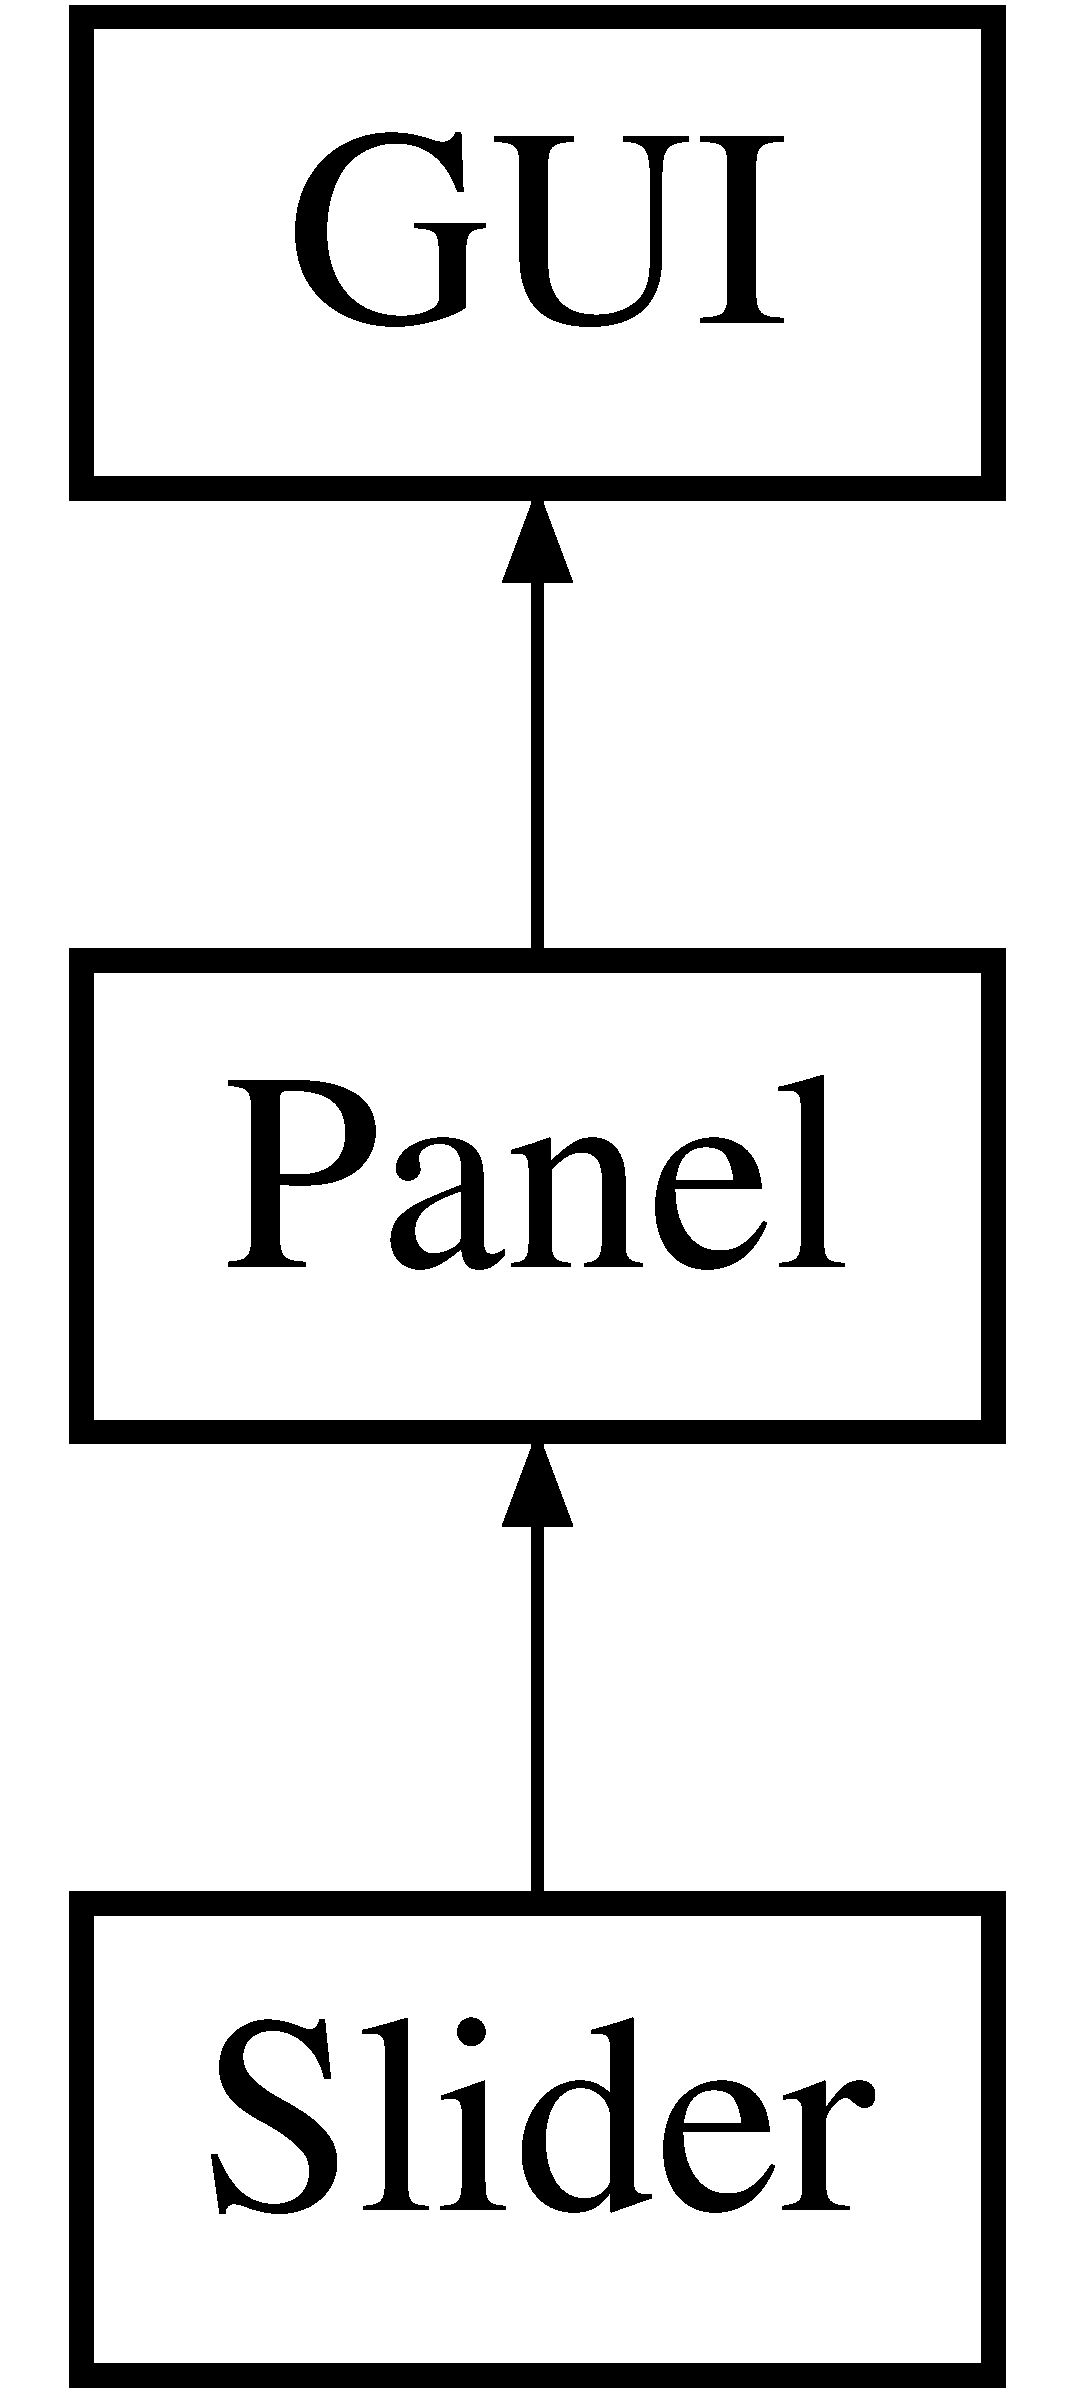
\includegraphics[height=3.000000cm]{class_slider}
\end{center}
\end{figure}
\subsection*{Public Member Functions}
\begin{DoxyCompactItemize}
\item 
\mbox{\hyperlink{class_slider_ad9bceb3f462c084a91bfe910065fe94f}{Slider}} (float \mbox{\hyperlink{class_g_u_i_a7fa193a8ffb27bbb3bcc225e36f6d54d}{x}}, float \mbox{\hyperlink{class_g_u_i_a98f204f99ffc5ff6cffc9340bbb8c29b}{y}}, float \mbox{\hyperlink{class_g_u_i_aee5d8766834f6f743f0d8b8c16e47155}{width}}, float \mbox{\hyperlink{class_g_u_i_a70b578c36323a45cac88ccff3bced933}{height}}, \mbox{\hyperlink{class_vector4}{Vector4F}} slider\+\_\+colour, \mbox{\hyperlink{class_vector4}{Vector4F}} background\+\_\+colour, \mbox{\hyperlink{class_vector2}{Vector2F}} slider\+\_\+size, \mbox{\hyperlink{class_shader}{Shader}} \&\mbox{\hyperlink{class_g_u_i_a64b007b31d0ec8a8704f9ab3bb2a7d3d}{shader}}, \mbox{\hyperlink{class_mouse_listener}{Mouse\+Listener}} \&mouse\+\_\+listener, float \mbox{\hyperlink{class_slider_ad699d9f4196d57dc18d1bdfd4d74bf67}{position}}=0.\+0f)
\item 
virtual void \mbox{\hyperlink{class_slider_a4ebd527db54ea263c7d0efe4d1f94e1b}{update}} () override
\item 
virtual bool \mbox{\hyperlink{class_slider_a30b01348a5d214f3078e22516c60a763}{focused}} () const override
\item 
virtual bool \mbox{\hyperlink{class_slider_a8d7d12aa4bc5d26de46790b43116bcc1}{is\+\_\+mouse\+\_\+sensitive}} () const override
\item 
bool \mbox{\hyperlink{class_slider_a736d0f12de097fa94f1b1b718f4f76a7}{moused\+\_\+over}} () const
\item 
bool \mbox{\hyperlink{class_slider_a59e849b069f0a02451e93a63884555c4}{clicked\+\_\+on}} () const
\item 
const \mbox{\hyperlink{class_vector4}{Vector4F}} \& \mbox{\hyperlink{class_slider_a660889686a2d0b9d73fb25cfb9eaff9a}{get\+\_\+slider\+\_\+colour}} () const
\item 
const \mbox{\hyperlink{class_vector2}{Vector2F}} \& \mbox{\hyperlink{class_slider_a235e764dfafeacc678b77f5300f44dba}{get\+\_\+slider\+\_\+size}} () const
\end{DoxyCompactItemize}
\subsection*{Public Attributes}
\begin{DoxyCompactItemize}
\item 
\mbox{\Hypertarget{class_slider_ad699d9f4196d57dc18d1bdfd4d74bf67}\label{class_slider_ad699d9f4196d57dc18d1bdfd4d74bf67}} 
double \mbox{\hyperlink{class_slider_ad699d9f4196d57dc18d1bdfd4d74bf67}{position}}
\begin{DoxyCompactList}\small\item\em Position of the slider wedge on the slider. Clamped between 0.\+0 and 1.\+0. \end{DoxyCompactList}\end{DoxyCompactItemize}
\subsection*{Additional Inherited Members}


\subsection{Detailed Description}
Graphical representation of a mutable double. Use this to enable user-\/input for editing continuous data. 

\subsection{Constructor \& Destructor Documentation}
\mbox{\Hypertarget{class_slider_ad9bceb3f462c084a91bfe910065fe94f}\label{class_slider_ad9bceb3f462c084a91bfe910065fe94f}} 
\index{Slider@{Slider}!Slider@{Slider}}
\index{Slider@{Slider}!Slider@{Slider}}
\subsubsection{\texorpdfstring{Slider()}{Slider()}}
{\footnotesize\ttfamily Slider\+::\+Slider (\begin{DoxyParamCaption}\item[{float}]{x,  }\item[{float}]{y,  }\item[{float}]{width,  }\item[{float}]{height,  }\item[{\mbox{\hyperlink{class_vector4}{Vector4F}}}]{slider\+\_\+colour,  }\item[{\mbox{\hyperlink{class_vector4}{Vector4F}}}]{background\+\_\+colour,  }\item[{\mbox{\hyperlink{class_vector2}{Vector2F}}}]{slider\+\_\+size,  }\item[{\mbox{\hyperlink{class_shader}{Shader}} \&}]{shader,  }\item[{\mbox{\hyperlink{class_mouse_listener}{Mouse\+Listener}} \&}]{mouse\+\_\+listener,  }\item[{float}]{position = {\ttfamily 0.0f} }\end{DoxyParamCaption})}

Construct a \mbox{\hyperlink{class_slider}{Slider}} with all specifications. 
\begin{DoxyParams}{Parameters}
{\em x} & -\/ Position of the slider on the x-\/axis, in pixels \\
\hline
{\em y} & -\/ Position of the slider on the y-\/axis, in pixels \\
\hline
{\em width} & -\/ Width of the slider, in pixels \\
\hline
{\em height} & -\/ Height of the slider, in pixels \\
\hline
{\em slider\+\_\+colour} & -\/ Colour of the slider\textquotesingle{}s wedge. \\
\hline
{\em background\+\_\+colour} & -\/ Background colour of the slider body. \\
\hline
{\em slider\+\_\+size} & -\/ 2-\/dimensional \mbox{\hyperlink{class_vector}{Vector}} representing the size of the slider\textquotesingle{}s wedge. \\
\hline
{\em shader} & -\/ The shader with which to render the slider. \\
\hline
{\em mouse\+\_\+listener} & -\/ The mouse-\/listener with which to query whether the slider needs to have its wedge dragged \\
\hline
{\em position} & -\/ Current position of the slider wedge, clamped between 0.\+0 and 1.\+0 \\
\hline
\end{DoxyParams}


\subsection{Member Function Documentation}
\mbox{\Hypertarget{class_slider_a59e849b069f0a02451e93a63884555c4}\label{class_slider_a59e849b069f0a02451e93a63884555c4}} 
\index{Slider@{Slider}!clicked\+\_\+on@{clicked\+\_\+on}}
\index{clicked\+\_\+on@{clicked\+\_\+on}!Slider@{Slider}}
\subsubsection{\texorpdfstring{clicked\+\_\+on()}{clicked\_on()}}
{\footnotesize\ttfamily bool Slider\+::clicked\+\_\+on (\begin{DoxyParamCaption}{ }\end{DoxyParamCaption}) const}

Query whether the slider is currently being clicked on. \begin{DoxyReturn}{Returns}
-\/ True if the slider is being clicked on. False otherwise 
\end{DoxyReturn}
\mbox{\Hypertarget{class_slider_a30b01348a5d214f3078e22516c60a763}\label{class_slider_a30b01348a5d214f3078e22516c60a763}} 
\index{Slider@{Slider}!focused@{focused}}
\index{focused@{focused}!Slider@{Slider}}
\subsubsection{\texorpdfstring{focused()}{focused()}}
{\footnotesize\ttfamily bool Slider\+::focused (\begin{DoxyParamCaption}{ }\end{DoxyParamCaption}) const\hspace{0.3cm}{\ttfamily [override]}, {\ttfamily [virtual]}}

Query whether the slider is currently focused. \begin{DoxyReturn}{Returns}
-\/ True if the slider is focused. False otherwise 
\end{DoxyReturn}


Reimplemented from \mbox{\hyperlink{class_panel_ace2217419ea5c2e98a38678c6e2012e1}{Panel}}.

\mbox{\Hypertarget{class_slider_a660889686a2d0b9d73fb25cfb9eaff9a}\label{class_slider_a660889686a2d0b9d73fb25cfb9eaff9a}} 
\index{Slider@{Slider}!get\+\_\+slider\+\_\+colour@{get\+\_\+slider\+\_\+colour}}
\index{get\+\_\+slider\+\_\+colour@{get\+\_\+slider\+\_\+colour}!Slider@{Slider}}
\subsubsection{\texorpdfstring{get\+\_\+slider\+\_\+colour()}{get\_slider\_colour()}}
{\footnotesize\ttfamily const \mbox{\hyperlink{class_vector4}{Vector4F}} \& Slider\+::get\+\_\+slider\+\_\+colour (\begin{DoxyParamCaption}{ }\end{DoxyParamCaption}) const}

Get the R\+G\+B\+A-\/coded colour of the slider wedge. \begin{DoxyReturn}{Returns}
-\/ Colour of the slider wegde. 
\end{DoxyReturn}
\mbox{\Hypertarget{class_slider_a235e764dfafeacc678b77f5300f44dba}\label{class_slider_a235e764dfafeacc678b77f5300f44dba}} 
\index{Slider@{Slider}!get\+\_\+slider\+\_\+size@{get\+\_\+slider\+\_\+size}}
\index{get\+\_\+slider\+\_\+size@{get\+\_\+slider\+\_\+size}!Slider@{Slider}}
\subsubsection{\texorpdfstring{get\+\_\+slider\+\_\+size()}{get\_slider\_size()}}
{\footnotesize\ttfamily const \mbox{\hyperlink{class_vector2}{Vector2F}} \& Slider\+::get\+\_\+slider\+\_\+size (\begin{DoxyParamCaption}{ }\end{DoxyParamCaption}) const}

Get the dimensions of the slider. \begin{DoxyReturn}{Returns}
-\/ 2-\/dimensional \mbox{\hyperlink{class_vector}{Vector}} representing the size of the wedge of the slider. 
\end{DoxyReturn}
\mbox{\Hypertarget{class_slider_a8d7d12aa4bc5d26de46790b43116bcc1}\label{class_slider_a8d7d12aa4bc5d26de46790b43116bcc1}} 
\index{Slider@{Slider}!is\+\_\+mouse\+\_\+sensitive@{is\+\_\+mouse\+\_\+sensitive}}
\index{is\+\_\+mouse\+\_\+sensitive@{is\+\_\+mouse\+\_\+sensitive}!Slider@{Slider}}
\subsubsection{\texorpdfstring{is\+\_\+mouse\+\_\+sensitive()}{is\_mouse\_sensitive()}}
{\footnotesize\ttfamily virtual bool Slider\+::is\+\_\+mouse\+\_\+sensitive (\begin{DoxyParamCaption}{ }\end{DoxyParamCaption}) const\hspace{0.3cm}{\ttfamily [inline]}, {\ttfamily [override]}, {\ttfamily [virtual]}}

Sliders are mouse-\/sensitive. \begin{DoxyReturn}{Returns}
-\/ True 
\end{DoxyReturn}


Reimplemented from \mbox{\hyperlink{class_panel_a607fe6e1be6fd056f199fa817a4dedda}{Panel}}.

\mbox{\Hypertarget{class_slider_a736d0f12de097fa94f1b1b718f4f76a7}\label{class_slider_a736d0f12de097fa94f1b1b718f4f76a7}} 
\index{Slider@{Slider}!moused\+\_\+over@{moused\+\_\+over}}
\index{moused\+\_\+over@{moused\+\_\+over}!Slider@{Slider}}
\subsubsection{\texorpdfstring{moused\+\_\+over()}{moused\_over()}}
{\footnotesize\ttfamily bool Slider\+::moused\+\_\+over (\begin{DoxyParamCaption}{ }\end{DoxyParamCaption}) const}

Query whether the slider is currently being moused-\/over. \begin{DoxyReturn}{Returns}
-\/ True if the slider is moused-\/over. False otherwise 
\end{DoxyReturn}
\mbox{\Hypertarget{class_slider_a4ebd527db54ea263c7d0efe4d1f94e1b}\label{class_slider_a4ebd527db54ea263c7d0efe4d1f94e1b}} 
\index{Slider@{Slider}!update@{update}}
\index{update@{update}!Slider@{Slider}}
\subsubsection{\texorpdfstring{update()}{update()}}
{\footnotesize\ttfamily void Slider\+::update (\begin{DoxyParamCaption}{ }\end{DoxyParamCaption})\hspace{0.3cm}{\ttfamily [override]}, {\ttfamily [virtual]}}

Render and update all children. 

Reimplemented from \mbox{\hyperlink{class_panel_a9e9c0608cf3139833cde6b73dc3ba443}{Panel}}.



The documentation for this class was generated from the following files\+:\begin{DoxyCompactItemize}
\item 
src/graphics/gui\+\_\+widget.\+hpp\item 
src/graphics/gui\+\_\+widget.\+cpp\end{DoxyCompactItemize}

\hypertarget{class_sprite}{}\section{Sprite Class Reference}
\label{class_sprite}\index{Sprite@{Sprite}}


{\ttfamily \#include $<$sprite.\+hpp$>$}

Inheritance diagram for Sprite\+:\begin{figure}[H]
\begin{center}
\leavevmode
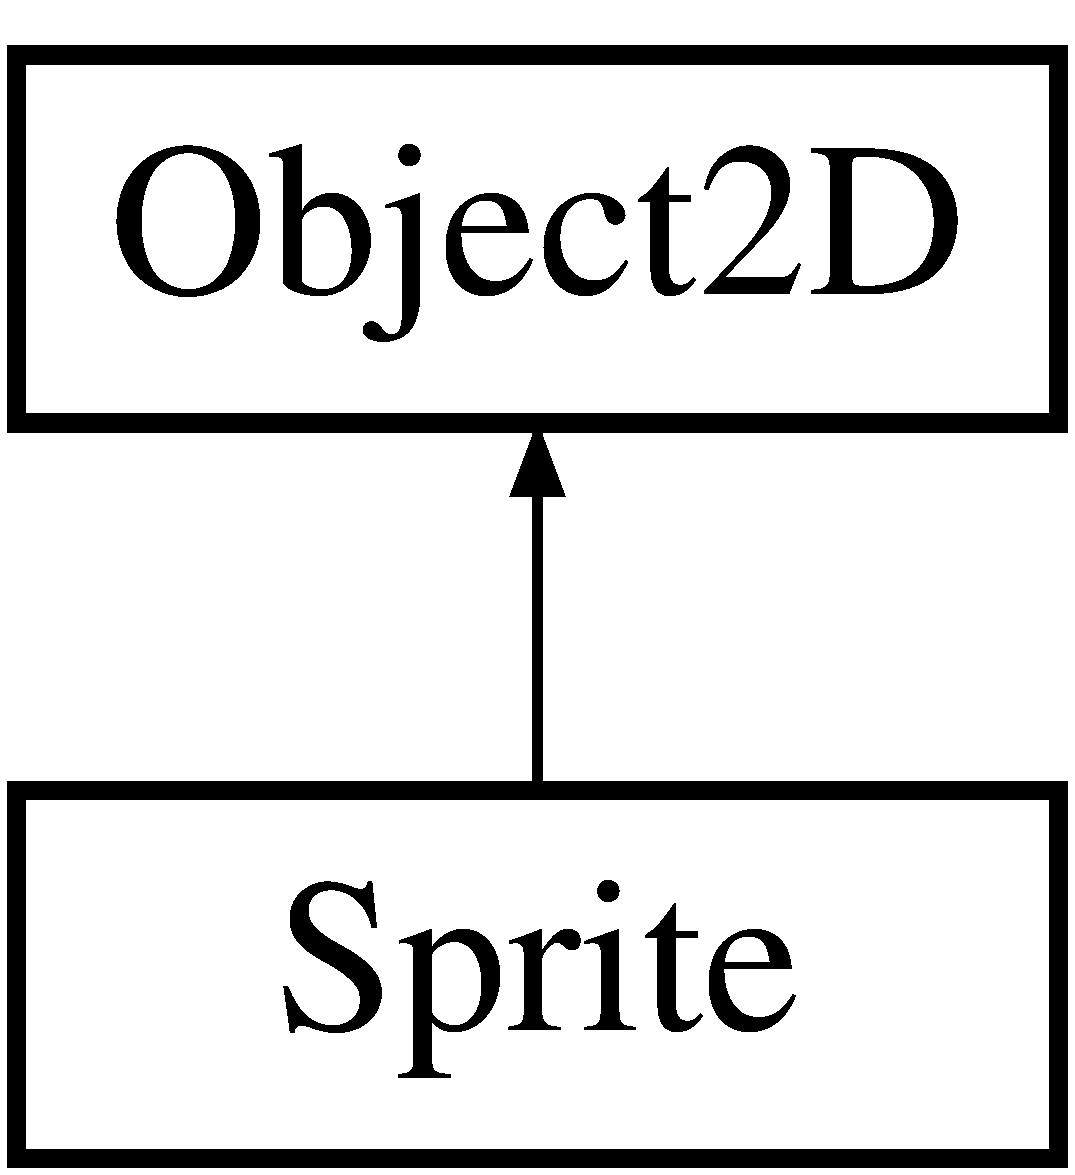
\includegraphics[height=2.000000cm]{class_sprite}
\end{center}
\end{figure}
\subsection*{Public Member Functions}
\begin{DoxyCompactItemize}
\item 
\mbox{\Hypertarget{class_sprite_a555482129461dfe0f4f296ea2e78f153}\label{class_sprite_a555482129461dfe0f4f296ea2e78f153}} 
{\bfseries Sprite} (\mbox{\hyperlink{class_vector2}{Vector2F}} position, float rotation, \mbox{\hyperlink{class_vector2}{Vector2F}} scale, const \mbox{\hyperlink{class_texture}{Texture}} $\ast$texture)
\item 
\mbox{\Hypertarget{class_sprite_ac32f104ca4bc443adbdfc53bec082a34}\label{class_sprite_ac32f104ca4bc443adbdfc53bec082a34}} 
{\bfseries Sprite} (\mbox{\hyperlink{class_vector2}{Vector2F}} position, float rotation, \mbox{\hyperlink{class_vector2}{Vector2F}} scale, \mbox{\hyperlink{class_vector4}{Vector4F}} colour)
\item 
\mbox{\Hypertarget{class_sprite_a2937195112c58787f249689324456c9f}\label{class_sprite_a2937195112c58787f249689324456c9f}} 
\mbox{\hyperlink{class_sprite}{Sprite}} \& {\bfseries operator=} (const \mbox{\hyperlink{class_sprite}{Sprite}} \&copy)
\item 
\mbox{\Hypertarget{class_sprite_a93a83d6c6941cff4036c50110d1b1ec4}\label{class_sprite_a93a83d6c6941cff4036c50110d1b1ec4}} 
virtual void {\bfseries render} (const \mbox{\hyperlink{class_camera}{Camera}} \&cam, \mbox{\hyperlink{class_shader}{Shader}} $\ast$shader, float width, float height) const override
\end{DoxyCompactItemize}
\subsection*{Additional Inherited Members}


\subsection{Detailed Description}
Like a normal \mbox{\hyperlink{class_object2_d}{Object2D}}, but has a texture bound. 

The documentation for this class was generated from the following files\+:\begin{DoxyCompactItemize}
\item 
src/graphics/sprite.\+hpp\item 
src/graphics/sprite.\+cpp\end{DoxyCompactItemize}

\hypertarget{class_static_functor}{}\section{Static\+Functor$<$ Functor, Functor\+Parameters $>$ Class Template Reference}
\label{class_static_functor}\index{Static\+Functor$<$ Functor, Functor\+Parameters $>$@{Static\+Functor$<$ Functor, Functor\+Parameters $>$}}


{\ttfamily \#include $<$command.\+hpp$>$}

Inheritance diagram for Static\+Functor$<$ Functor, Functor\+Parameters $>$\+:\begin{figure}[H]
\begin{center}
\leavevmode
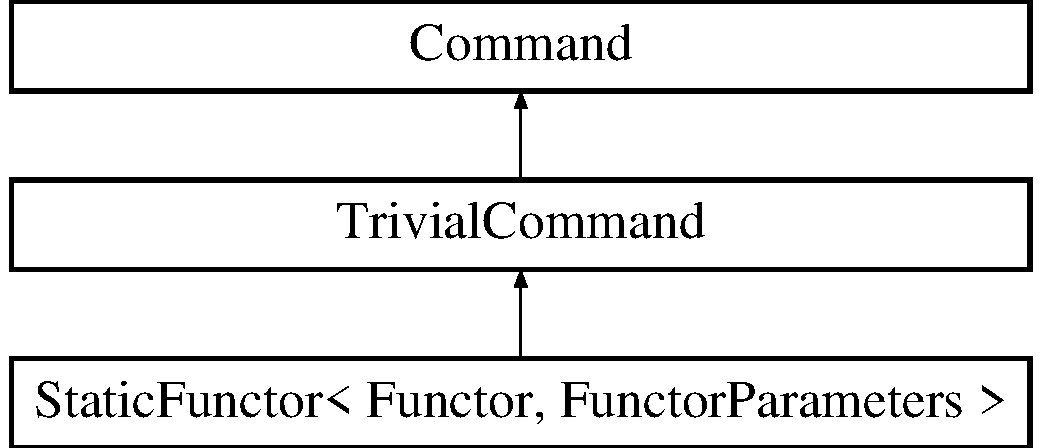
\includegraphics[height=3.000000cm]{class_static_functor}
\end{center}
\end{figure}
\subsection*{Public Member Functions}
\begin{DoxyCompactItemize}
\item 
\mbox{\hyperlink{class_static_functor_a61ee85704ebc97245006d4d8801fd58f}{Static\+Functor}} (\mbox{\hyperlink{class_functor}{Functor}} \&\&\mbox{\hyperlink{class_static_functor_aea8563c235a2dea8474da84504c51b58}{functor}}, Functor\+Parameters \&\&... \mbox{\hyperlink{class_static_functor_aaa5d69cb0c000ea6c4846296de2c7f7f}{parameters}})
\item 
virtual void \mbox{\hyperlink{class_static_functor_a1d8fe0ec2f9965c5f95ad182a8df510b}{operator()}} () override
\end{DoxyCompactItemize}
\subsection*{Protected Attributes}
\begin{DoxyCompactItemize}
\item 
\mbox{\Hypertarget{class_static_functor_aea8563c235a2dea8474da84504c51b58}\label{class_static_functor_aea8563c235a2dea8474da84504c51b58}} 
\mbox{\hyperlink{class_functor}{Functor}} \mbox{\hyperlink{class_static_functor_aea8563c235a2dea8474da84504c51b58}{functor}}
\begin{DoxyCompactList}\small\item\em The underlying functor. \end{DoxyCompactList}\item 
\mbox{\Hypertarget{class_static_functor_aaa5d69cb0c000ea6c4846296de2c7f7f}\label{class_static_functor_aaa5d69cb0c000ea6c4846296de2c7f7f}} 
std\+::tuple$<$ Functor\+Parameters... $>$ \mbox{\hyperlink{class_static_functor_aaa5d69cb0c000ea6c4846296de2c7f7f}{parameters}}
\begin{DoxyCompactList}\small\item\em Tuple containing all the parameters to be used when the functor is executed. \end{DoxyCompactList}\end{DoxyCompactItemize}


\subsection{Detailed Description}
\subsubsection*{template$<$typename Functor, typename... Functor\+Parameters$>$\newline
class Static\+Functor$<$ Functor, Functor\+Parameters $>$}

Represent a \mbox{\hyperlink{class_functor}{Functor}} storing all its arguments upon construction. 
\begin{DoxyTemplParams}{Template Parameters}
{\em \mbox{\hyperlink{class_functor}{Functor}}} & -\/ Type of the underlying functor. \\
\hline
{\em Functor\+Parameters} & -\/ Template parameter pack representing argument types. \\
\hline
\end{DoxyTemplParams}


\subsection{Constructor \& Destructor Documentation}
\mbox{\Hypertarget{class_static_functor_a61ee85704ebc97245006d4d8801fd58f}\label{class_static_functor_a61ee85704ebc97245006d4d8801fd58f}} 
\index{Static\+Functor@{Static\+Functor}!Static\+Functor@{Static\+Functor}}
\index{Static\+Functor@{Static\+Functor}!Static\+Functor@{Static\+Functor}}
\subsubsection{\texorpdfstring{Static\+Functor()}{StaticFunctor()}}
{\footnotesize\ttfamily template$<$typename Functor , typename... Functor\+Parameters$>$ \\
\mbox{\hyperlink{class_static_functor}{Static\+Functor}}$<$ \mbox{\hyperlink{class_functor}{Functor}}, Functor\+Parameters $>$\+::\mbox{\hyperlink{class_static_functor}{Static\+Functor}} (\begin{DoxyParamCaption}\item[{\mbox{\hyperlink{class_functor}{Functor}} \&\&}]{functor,  }\item[{Functor\+Parameters \&\&...}]{parameters }\end{DoxyParamCaption})}

Construct a \mbox{\hyperlink{class_static_functor}{Static\+Functor}} from an underlying functor and all the parameters it requires. 
\begin{DoxyParams}{Parameters}
{\em functor} & -\/ The underlying functor \\
\hline
{\em parameters} & -\/ Variadic parameters representing parameters of the \mbox{\hyperlink{class_static_functor}{Static\+Functor}}. These are stored in the \mbox{\hyperlink{class_static_functor}{Static\+Functor}}. \\
\hline
\end{DoxyParams}


\subsection{Member Function Documentation}
\mbox{\Hypertarget{class_static_functor_a1d8fe0ec2f9965c5f95ad182a8df510b}\label{class_static_functor_a1d8fe0ec2f9965c5f95ad182a8df510b}} 
\index{Static\+Functor@{Static\+Functor}!operator()@{operator()}}
\index{operator()@{operator()}!Static\+Functor@{Static\+Functor}}
\subsubsection{\texorpdfstring{operator()()}{operator()()}}
{\footnotesize\ttfamily template$<$typename Functor , typename... Functor\+Parameters$>$ \\
void \mbox{\hyperlink{class_static_functor}{Static\+Functor}}$<$ \mbox{\hyperlink{class_functor}{Functor}}, Functor\+Parameters $>$\+::operator() (\begin{DoxyParamCaption}{ }\end{DoxyParamCaption})\hspace{0.3cm}{\ttfamily [override]}, {\ttfamily [virtual]}}

Invoked when the \mbox{\hyperlink{class_static_functor}{Static\+Functor}} is executed. Runs the underlying functor with all variadic parameters. 

Implements \mbox{\hyperlink{class_trivial_command_aa61a3e5fd78d3a2dec6fcf6dcb2e5189}{Trivial\+Command}}.



The documentation for this class was generated from the following files\+:\begin{DoxyCompactItemize}
\item 
src/command.\+hpp\item 
src/command.\+inl\end{DoxyCompactItemize}

\hypertarget{structstbi__io__callbacks}{}\section{stbi\+\_\+io\+\_\+callbacks Struct Reference}
\label{structstbi__io__callbacks}\index{stbi\+\_\+io\+\_\+callbacks@{stbi\+\_\+io\+\_\+callbacks}}
\subsection*{Public Attributes}
\begin{DoxyCompactItemize}
\item 
\mbox{\Hypertarget{structstbi__io__callbacks_a623e46b3a2a019611601409926283a88}\label{structstbi__io__callbacks_a623e46b3a2a019611601409926283a88}} 
int($\ast$ {\bfseries read} )(void $\ast$user, char $\ast$data, int size)
\item 
\mbox{\Hypertarget{structstbi__io__callbacks_a257aac5480a90a6c4b8fbe86c1b01068}\label{structstbi__io__callbacks_a257aac5480a90a6c4b8fbe86c1b01068}} 
void($\ast$ {\bfseries skip} )(void $\ast$user, int n)
\item 
\mbox{\Hypertarget{structstbi__io__callbacks_a319639db2f76e715eed7a7a974136832}\label{structstbi__io__callbacks_a319639db2f76e715eed7a7a974136832}} 
int($\ast$ {\bfseries eof} )(void $\ast$user)
\end{DoxyCompactItemize}


The documentation for this struct was generated from the following file\+:\begin{DoxyCompactItemize}
\item 
src/graphics/stb\+\_\+image.\+h\end{DoxyCompactItemize}

\hypertarget{class_text_label}{}\section{Text\+Label Class Reference}
\label{class_text_label}\index{Text\+Label@{Text\+Label}}


{\ttfamily \#include $<$gui\+\_\+display.\+hpp$>$}

Inheritance diagram for Text\+Label\+:\begin{figure}[H]
\begin{center}
\leavevmode
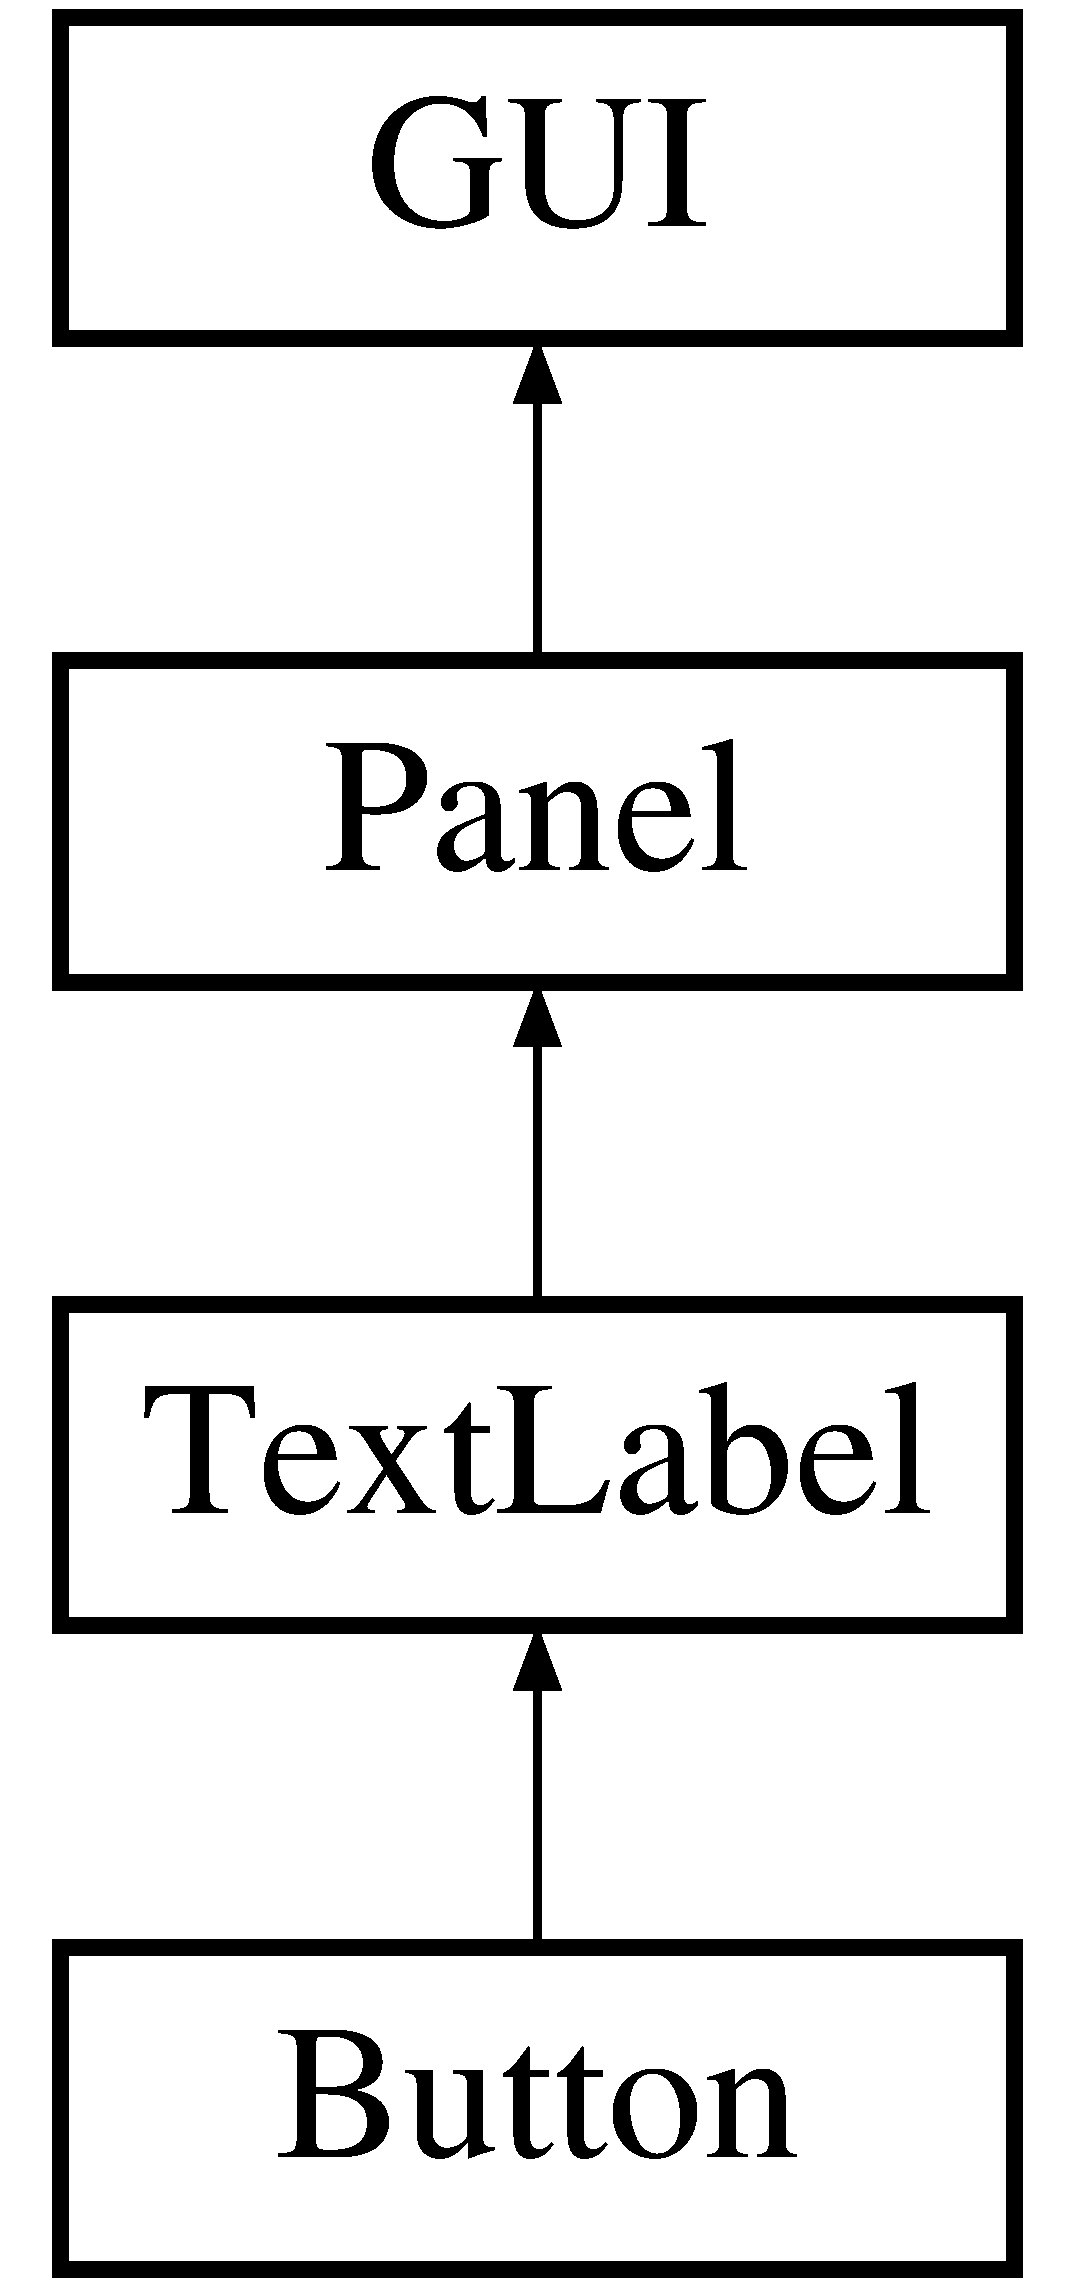
\includegraphics[height=4.000000cm]{class_text_label}
\end{center}
\end{figure}
\subsection*{Public Member Functions}
\begin{DoxyCompactItemize}
\item 
\mbox{\Hypertarget{class_text_label_a8736731b5c5f1a8cffa984cfc332a859}\label{class_text_label_a8736731b5c5f1a8cffa984cfc332a859}} 
{\bfseries Text\+Label} (float x, float y, \mbox{\hyperlink{class_vector4}{Vector4F}} colour, std\+::optional$<$ \mbox{\hyperlink{class_vector4}{Vector4F}} $>$ background\+\_\+colour, std\+::optional$<$ \mbox{\hyperlink{class_vector3}{Vector3F}} $>$ text\+\_\+border\+\_\+colour, \mbox{\hyperlink{class_font}{Font}} font, const std\+::string \&text, \mbox{\hyperlink{class_shader}{Shader}} \&shader)
\item 
\mbox{\Hypertarget{class_text_label_ae2d0c39b245449882cc66519acf6c6aa}\label{class_text_label_ae2d0c39b245449882cc66519acf6c6aa}} 
{\bfseries Text\+Label} (const \mbox{\hyperlink{class_text_label}{Text\+Label}} \&copy)=default
\item 
\mbox{\Hypertarget{class_text_label_a27045baf12d91734102eca29411c71b5}\label{class_text_label_a27045baf12d91734102eca29411c71b5}} 
{\bfseries Text\+Label} (\mbox{\hyperlink{class_text_label}{Text\+Label}} \&\&move)=default
\item 
\mbox{\Hypertarget{class_text_label_ad8cfeadea1dd3d1a869f5b8ef1e9eb70}\label{class_text_label_ad8cfeadea1dd3d1a869f5b8ef1e9eb70}} 
\mbox{\hyperlink{class_text_label}{Text\+Label}} \& {\bfseries operator=} (const \mbox{\hyperlink{class_text_label}{Text\+Label}} \&rhs)=default
\item 
\mbox{\Hypertarget{class_text_label_a350a9edc23e4d2a53374fddc5ddc61cc}\label{class_text_label_a350a9edc23e4d2a53374fddc5ddc61cc}} 
virtual void {\bfseries update} () override
\item 
\mbox{\Hypertarget{class_text_label_a551d9e453aed5769c47bf815f3954b87}\label{class_text_label_a551d9e453aed5769c47bf815f3954b87}} 
bool {\bfseries has\+\_\+background\+\_\+colour} () const
\item 
\mbox{\Hypertarget{class_text_label_a3ebd1440ba16deddd630f59e32def63e}\label{class_text_label_a3ebd1440ba16deddd630f59e32def63e}} 
bool {\bfseries has\+\_\+text\+\_\+border\+\_\+colour} () const
\item 
\mbox{\Hypertarget{class_text_label_a9cf910ea092dd7b72c53a028e9ae3998}\label{class_text_label_a9cf910ea092dd7b72c53a028e9ae3998}} 
const \mbox{\hyperlink{class_font}{Font}} \& {\bfseries get\+\_\+font} () const
\item 
\mbox{\Hypertarget{class_text_label_a899b24fdb8ce8adf213cb70461aa1d91}\label{class_text_label_a899b24fdb8ce8adf213cb70461aa1d91}} 
void {\bfseries set\+\_\+font} (\mbox{\hyperlink{class_font}{Font}} font)
\item 
\mbox{\Hypertarget{class_text_label_a3594731b87e5c98a5d574e554e4ebcf0}\label{class_text_label_a3594731b87e5c98a5d574e554e4ebcf0}} 
const std\+::string \& {\bfseries get\+\_\+text} () const
\item 
\mbox{\Hypertarget{class_text_label_ad8d83bed9697b2f53249218f560fe1a8}\label{class_text_label_ad8d83bed9697b2f53249218f560fe1a8}} 
void {\bfseries set\+\_\+text} (const std\+::string \&new\+\_\+text)
\item 
\mbox{\Hypertarget{class_text_label_ab8af6195b3e568d5f8a83024818b6d80}\label{class_text_label_ab8af6195b3e568d5f8a83024818b6d80}} 
const \mbox{\hyperlink{class_texture}{Texture}} \& {\bfseries get\+\_\+texture} () const
\item 
\mbox{\Hypertarget{class_text_label_ae39dffa6e09e0ef03f2ef8f980e47076}\label{class_text_label_ae39dffa6e09e0ef03f2ef8f980e47076}} 
void {\bfseries set\+\_\+texture} (\mbox{\hyperlink{class_texture}{Texture}} texture)
\end{DoxyCompactItemize}
\subsection*{Additional Inherited Members}


\subsection{Detailed Description}
Very similar to a \mbox{\hyperlink{class_panel}{Panel}}, but has additional font-\/rendering applied. Use this to write text to the screen. 

The documentation for this class was generated from the following files\+:\begin{DoxyCompactItemize}
\item 
src/graphics/gui\+\_\+display.\+hpp\item 
src/graphics/gui\+\_\+display.\+cpp\end{DoxyCompactItemize}

\hypertarget{class_texture}{}\section{Texture Class Reference}
\label{class_texture}\index{Texture@{Texture}}


{\ttfamily \#include $<$texture.\+hpp$>$}

Inheritance diagram for Texture\+:\begin{figure}[H]
\begin{center}
\leavevmode
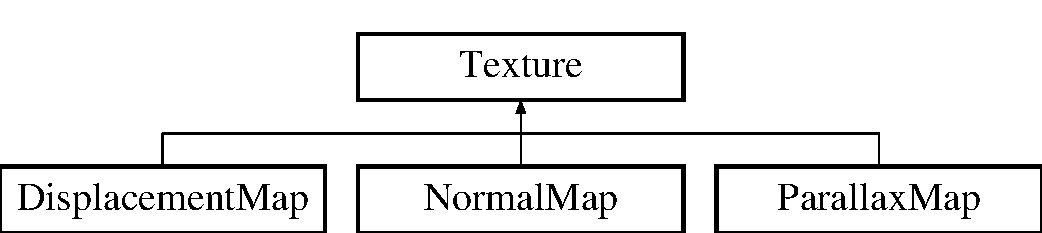
\includegraphics[height=2.000000cm]{class_texture}
\end{center}
\end{figure}
\subsection*{Public Member Functions}
\begin{DoxyCompactItemize}
\item 
\mbox{\hyperlink{class_texture_a6c275e3f186675ff6ed73ccf970e552f}{Texture}} ()
\item 
\mbox{\hyperlink{class_texture_a197b839d8525505209f4288071cc7185}{Texture}} (int width, int height)
\item 
\mbox{\hyperlink{class_texture_a84ada24c7d5dec8fca128752a6459106}{Texture}} (std\+::string filename, bool mipmapping=true, bool gamma\+\_\+corrected=true, bool store\+\_\+bitmap=false)
\item 
{\footnotesize template$<$class Pixel $>$ }\\\mbox{\hyperlink{class_texture_a503b9fb36275ab110763bf9f51420539}{Texture}} (\mbox{\hyperlink{class_bitmap}{Bitmap}}$<$ Pixel $>$ pixel\+\_\+data)
\item 
\mbox{\hyperlink{class_texture_a38ee78c007ed592860dc4c35948f57da}{Texture}} (const \mbox{\hyperlink{class_font}{Font}} \&font, const std\+::string \&text, S\+D\+L\+\_\+\+Color foreground\+\_\+colour, bool store\+\_\+bitmap=false)
\item 
\mbox{\Hypertarget{class_texture_abdf82a7e3262db9452fb0fd994d01c69}\label{class_texture_abdf82a7e3262db9452fb0fd994d01c69}} 
{\bfseries Texture} (const \mbox{\hyperlink{class_texture}{Texture}} \&copy)
\item 
\mbox{\Hypertarget{class_texture_a3509443fca1d7a53de22fa83d7f882a2}\label{class_texture_a3509443fca1d7a53de22fa83d7f882a2}} 
{\bfseries Texture} (\mbox{\hyperlink{class_texture}{Texture}} \&\&move)
\item 
\mbox{\Hypertarget{class_texture_a18d2cb10fecc26f4b6692b04d877cafa}\label{class_texture_a18d2cb10fecc26f4b6692b04d877cafa}} 
\mbox{\hyperlink{class_texture}{Texture}} \& {\bfseries operator=} (\mbox{\hyperlink{class_texture}{Texture}} \&\&rhs)
\item 
\mbox{\Hypertarget{class_texture_ac8ae77bfd20815c814606ad179835ec4}\label{class_texture_ac8ae77bfd20815c814606ad179835ec4}} 
virtual void {\bfseries bind} (\mbox{\hyperlink{class_shader}{Shader}} $\ast$shader, unsigned int id) const
\item 
\mbox{\Hypertarget{class_texture_aa254021d42806acb75447992acdef0b0}\label{class_texture_aa254021d42806acb75447992acdef0b0}} 
bool {\bfseries has\+\_\+file\+\_\+name} () const
\item 
\mbox{\Hypertarget{class_texture_a1997024a190c49b1a9405788aa79fdcd}\label{class_texture_a1997024a190c49b1a9405788aa79fdcd}} 
const std\+::string \& {\bfseries get\+\_\+file\+\_\+name} () const
\item 
\mbox{\Hypertarget{class_texture_a0855aaa1c0252620681351b1cf8f2244}\label{class_texture_a0855aaa1c0252620681351b1cf8f2244}} 
int {\bfseries get\+\_\+width} () const
\item 
\mbox{\Hypertarget{class_texture_a04e93b660b6588087569275641417d51}\label{class_texture_a04e93b660b6588087569275641417d51}} 
int {\bfseries get\+\_\+height} () const
\item 
\mbox{\Hypertarget{class_texture_a7d569e6b184fb98307a97086d0ab74b8}\label{class_texture_a7d569e6b184fb98307a97086d0ab74b8}} 
bool {\bfseries has\+\_\+bitmap} () const
\item 
\mbox{\Hypertarget{class_texture_ab33e71e57ac4fd800e3f171854748dad}\label{class_texture_ab33e71e57ac4fd800e3f171854748dad}} 
tz\+::graphics\+::\+Mipmap\+Type {\bfseries get\+\_\+mipmap\+\_\+type} () const
\item 
\mbox{\Hypertarget{class_texture_a8c93ccbbcf6c1c4710e89f8eb45ce500}\label{class_texture_a8c93ccbbcf6c1c4710e89f8eb45ce500}} 
bool {\bfseries has\+\_\+mipmap} () const
\item 
\mbox{\Hypertarget{class_texture_aa5ee6e7456b6d68918f6814eef76f7ac}\label{class_texture_aa5ee6e7456b6d68918f6814eef76f7ac}} 
\mbox{\hyperlink{class_bitmap}{Bitmap}}$<$ \mbox{\hyperlink{class_pixel_r_g_b_a}{Pixel\+R\+G\+BA}} $>$ {\bfseries get\+\_\+bitmap} () const
\item 
\mbox{\Hypertarget{class_texture_a1f0034e4e96f51539165bfc861d5c7c9}\label{class_texture_a1f0034e4e96f51539165bfc861d5c7c9}} 
virtual tz\+::graphics\+::\+Texture\+Type {\bfseries get\+\_\+texture\+\_\+type} () const
\item 
\mbox{\Hypertarget{class_texture_a8a8184cc15e59a78e64131773f1da839}\label{class_texture_a8a8184cc15e59a78e64131773f1da839}} 
bool {\bfseries operator==} (const \mbox{\hyperlink{class_texture}{Texture}} \&rhs) const
\end{DoxyCompactItemize}
\subsection*{Static Public Member Functions}
\begin{DoxyCompactItemize}
\item 
\mbox{\Hypertarget{class_texture_a3b2d270058efab162df59cdfacd0c0c4}\label{class_texture_a3b2d270058efab162df59cdfacd0c0c4}} 
{\footnotesize template$<$class T $>$ }\\static T $\ast$ {\bfseries get\+\_\+from\+\_\+link} (const std\+::string \&texture\+\_\+link, const std\+::vector$<$ std\+::unique\+\_\+ptr$<$ T $>$$>$ \&all\+\_\+textures)
\end{DoxyCompactItemize}
\subsection*{Protected Member Functions}
\begin{DoxyCompactItemize}
\item 
\mbox{\Hypertarget{class_texture_a10c263cedc41ebaf472ff5f424a28130}\label{class_texture_a10c263cedc41ebaf472ff5f424a28130}} 
unsigned char $\ast$ {\bfseries load\+\_\+texture} ()
\item 
\mbox{\Hypertarget{class_texture_a9db7e7ba9d5866d0a58035df47b744e9}\label{class_texture_a9db7e7ba9d5866d0a58035df47b744e9}} 
void {\bfseries delete\+\_\+texture} (unsigned char $\ast$imgdata)
\item 
\mbox{\Hypertarget{class_texture_ab57990fdb5f5e053dcff6bea2c5e9f17}\label{class_texture_ab57990fdb5f5e053dcff6bea2c5e9f17}} 
void {\bfseries bind\+\_\+with\+\_\+string} (\mbox{\hyperlink{class_shader}{Shader}} $\ast$shader, unsigned int id, const std\+::string \&sampler\+\_\+uniform\+\_\+name) const
\end{DoxyCompactItemize}
\subsection*{Protected Attributes}
\begin{DoxyCompactItemize}
\item 
\mbox{\Hypertarget{class_texture_ad38f8ae3a9bf46ad60d461c58c53a614}\label{class_texture_ad38f8ae3a9bf46ad60d461c58c53a614}} 
std\+::optional$<$ std\+::string $>$ {\bfseries filename}
\item 
\mbox{\Hypertarget{class_texture_ae88a57598f85eaffe689b972c6436bcc}\label{class_texture_ae88a57598f85eaffe689b972c6436bcc}} 
G\+Luint {\bfseries texture\+\_\+handle}
\item 
\mbox{\Hypertarget{class_texture_a06a0246cb31343557c3441c5733349cd}\label{class_texture_a06a0246cb31343557c3441c5733349cd}} 
int {\bfseries width}
\item 
\mbox{\Hypertarget{class_texture_ad37c395c65ff8bde86230908027a6fcd}\label{class_texture_ad37c395c65ff8bde86230908027a6fcd}} 
int {\bfseries height}
\item 
\mbox{\Hypertarget{class_texture_a59c27456c7b83c7d0f95657195d65c43}\label{class_texture_a59c27456c7b83c7d0f95657195d65c43}} 
int {\bfseries components}
\item 
\mbox{\Hypertarget{class_texture_af386997e83dd758a3a7a3e2ff163ccbf}\label{class_texture_af386997e83dd758a3a7a3e2ff163ccbf}} 
bool {\bfseries gamma\+\_\+corrected}
\item 
\mbox{\Hypertarget{class_texture_ad9e439aa27032a8447b3f75d517784e1}\label{class_texture_ad9e439aa27032a8447b3f75d517784e1}} 
std\+::optional$<$ \mbox{\hyperlink{class_bitmap}{Bitmap}}$<$ \mbox{\hyperlink{class_pixel_r_g_b_a}{Pixel\+R\+G\+BA}} $>$ $>$ {\bfseries bitmap}
\end{DoxyCompactItemize}
\subsection*{Friends}
\begin{DoxyCompactItemize}
\item 
\mbox{\Hypertarget{class_texture_a7e815028687ed9f9e9e25851d8a17b27}\label{class_texture_a7e815028687ed9f9e9e25851d8a17b27}} 
class {\bfseries Frame\+Buffer}
\end{DoxyCompactItemize}


\subsection{Detailed Description}
Holds pixel and colour data and can interact with Open\+GL buffers. Bind Textures so that Topaz Meshes do not render monochromoatically. 

\subsection{Constructor \& Destructor Documentation}
\mbox{\Hypertarget{class_texture_a6c275e3f186675ff6ed73ccf970e552f}\label{class_texture_a6c275e3f186675ff6ed73ccf970e552f}} 
\index{Texture@{Texture}!Texture@{Texture}}
\index{Texture@{Texture}!Texture@{Texture}}
\subsubsection{\texorpdfstring{Texture()}{Texture()}\hspace{0.1cm}{\footnotesize\ttfamily [1/5]}}
{\footnotesize\ttfamily Texture\+::\+Texture (\begin{DoxyParamCaption}{ }\end{DoxyParamCaption})}

Creates an uninitialised texture. This allocates a texture-\/handle but nothing else, so is not ready for rendering. \mbox{\Hypertarget{class_texture_a197b839d8525505209f4288071cc7185}\label{class_texture_a197b839d8525505209f4288071cc7185}} 
\index{Texture@{Texture}!Texture@{Texture}}
\index{Texture@{Texture}!Texture@{Texture}}
\subsubsection{\texorpdfstring{Texture()}{Texture()}\hspace{0.1cm}{\footnotesize\ttfamily [2/5]}}
{\footnotesize\ttfamily Texture\+::\+Texture (\begin{DoxyParamCaption}\item[{int}]{width,  }\item[{int}]{height }\end{DoxyParamCaption})}

Creates a completely empty texture, but would be ready to be written to, if bound to a framebuffer. \mbox{\Hypertarget{class_texture_a84ada24c7d5dec8fca128752a6459106}\label{class_texture_a84ada24c7d5dec8fca128752a6459106}} 
\index{Texture@{Texture}!Texture@{Texture}}
\index{Texture@{Texture}!Texture@{Texture}}
\subsubsection{\texorpdfstring{Texture()}{Texture()}\hspace{0.1cm}{\footnotesize\ttfamily [3/5]}}
{\footnotesize\ttfamily Texture\+::\+Texture (\begin{DoxyParamCaption}\item[{std\+::string}]{filename,  }\item[{bool}]{mipmapping = {\ttfamily true},  }\item[{bool}]{gamma\+\_\+corrected = {\ttfamily true},  }\item[{bool}]{store\+\_\+bitmap = {\ttfamily false} }\end{DoxyParamCaption})}

Loads a texture from a file. \mbox{\Hypertarget{class_texture_a503b9fb36275ab110763bf9f51420539}\label{class_texture_a503b9fb36275ab110763bf9f51420539}} 
\index{Texture@{Texture}!Texture@{Texture}}
\index{Texture@{Texture}!Texture@{Texture}}
\subsubsection{\texorpdfstring{Texture()}{Texture()}\hspace{0.1cm}{\footnotesize\ttfamily [4/5]}}
{\footnotesize\ttfamily template$<$class Pixel $>$ \\
Texture\+::\+Texture (\begin{DoxyParamCaption}\item[{\mbox{\hyperlink{class_bitmap}{Bitmap}}$<$ Pixel $>$}]{pixel\+\_\+data }\end{DoxyParamCaption})}

Loads a texture from existing Pixel Data \mbox{\Hypertarget{class_texture_a38ee78c007ed592860dc4c35948f57da}\label{class_texture_a38ee78c007ed592860dc4c35948f57da}} 
\index{Texture@{Texture}!Texture@{Texture}}
\index{Texture@{Texture}!Texture@{Texture}}
\subsubsection{\texorpdfstring{Texture()}{Texture()}\hspace{0.1cm}{\footnotesize\ttfamily [5/5]}}
{\footnotesize\ttfamily Texture\+::\+Texture (\begin{DoxyParamCaption}\item[{const \mbox{\hyperlink{class_font}{Font}} \&}]{font,  }\item[{const std\+::string \&}]{text,  }\item[{S\+D\+L\+\_\+\+Color}]{foreground\+\_\+colour,  }\item[{bool}]{store\+\_\+bitmap = {\ttfamily false} }\end{DoxyParamCaption})}

Loads a texture from a font, given text. 

The documentation for this class was generated from the following files\+:\begin{DoxyCompactItemize}
\item 
src/graphics/texture.\+hpp\item 
src/graphics/texture.\+cpp\item 
src/graphics/texture.\+inl\end{DoxyCompactItemize}

\hypertarget{class_time_profiler}{}\section{Time\+Profiler Class Reference}
\label{class_time_profiler}\index{Time\+Profiler@{Time\+Profiler}}


{\ttfamily \#include $<$time.\+hpp$>$}

\subsection*{Public Member Functions}
\begin{DoxyCompactItemize}
\item 
\mbox{\Hypertarget{class_time_profiler_a9178bba0d24e58fee4aef9e3fab2d620}\label{class_time_profiler_a9178bba0d24e58fee4aef9e3fab2d620}} 
{\bfseries Time\+Profiler} (const \mbox{\hyperlink{class_time_profiler}{Time\+Profiler}} \&copy)=default
\item 
\mbox{\Hypertarget{class_time_profiler_a82cdfc8e60b457a7ea9a3566ca2138c3}\label{class_time_profiler_a82cdfc8e60b457a7ea9a3566ca2138c3}} 
{\bfseries Time\+Profiler} (\mbox{\hyperlink{class_time_profiler}{Time\+Profiler}} \&\&move)=default
\item 
\mbox{\Hypertarget{class_time_profiler_a0461511b6fdd47cb628c6866cb1d083f}\label{class_time_profiler_a0461511b6fdd47cb628c6866cb1d083f}} 
\mbox{\hyperlink{class_time_profiler}{Time\+Profiler}} \& {\bfseries operator=} (const \mbox{\hyperlink{class_time_profiler}{Time\+Profiler}} \&rhs)=default
\item 
void \mbox{\hyperlink{class_time_profiler_a336b6225fb048d7f0cccf4a7fc721bbb}{begin\+\_\+frame}} ()
\item 
void \mbox{\hyperlink{class_time_profiler_a51540762400c7493125ba3dbf5dfee4e}{end\+\_\+frame}} ()
\item 
void \mbox{\hyperlink{class_time_profiler_aaaccee940365a619c03f1f69a46803e4}{reset}} ()
\item 
float \mbox{\hyperlink{class_time_profiler_a6778c6545bc103055ee8e4e4bee57407}{get\+\_\+delta\+\_\+average}} () const
\item 
float \mbox{\hyperlink{class_time_profiler_a44468954e79b02942fb168b6597280a1}{get\+\_\+last\+\_\+delta}} () const
\item 
unsigned int \mbox{\hyperlink{class_time_profiler_a49dc639e9dd12ee6313707722f7e8ffe}{get\+\_\+fps}} () const
\end{DoxyCompactItemize}


\subsection{Detailed Description}
Specialised \mbox{\hyperlink{class_timer}{Timer}} that can be used to calculate F\+PS during runtime. 

\subsection{Member Function Documentation}
\mbox{\Hypertarget{class_time_profiler_a336b6225fb048d7f0cccf4a7fc721bbb}\label{class_time_profiler_a336b6225fb048d7f0cccf4a7fc721bbb}} 
\index{Time\+Profiler@{Time\+Profiler}!begin\+\_\+frame@{begin\+\_\+frame}}
\index{begin\+\_\+frame@{begin\+\_\+frame}!Time\+Profiler@{Time\+Profiler}}
\subsubsection{\texorpdfstring{begin\+\_\+frame()}{begin\_frame()}}
{\footnotesize\ttfamily void Time\+Profiler\+::begin\+\_\+frame (\begin{DoxyParamCaption}{ }\end{DoxyParamCaption})}

Invoke this at the beginning of your frame construction in the game-\/loop. \mbox{\Hypertarget{class_time_profiler_a51540762400c7493125ba3dbf5dfee4e}\label{class_time_profiler_a51540762400c7493125ba3dbf5dfee4e}} 
\index{Time\+Profiler@{Time\+Profiler}!end\+\_\+frame@{end\+\_\+frame}}
\index{end\+\_\+frame@{end\+\_\+frame}!Time\+Profiler@{Time\+Profiler}}
\subsubsection{\texorpdfstring{end\+\_\+frame()}{end\_frame()}}
{\footnotesize\ttfamily void Time\+Profiler\+::end\+\_\+frame (\begin{DoxyParamCaption}{ }\end{DoxyParamCaption})}

Invoke this at the end of your frame construction in the game-\/loop. \mbox{\Hypertarget{class_time_profiler_a6778c6545bc103055ee8e4e4bee57407}\label{class_time_profiler_a6778c6545bc103055ee8e4e4bee57407}} 
\index{Time\+Profiler@{Time\+Profiler}!get\+\_\+delta\+\_\+average@{get\+\_\+delta\+\_\+average}}
\index{get\+\_\+delta\+\_\+average@{get\+\_\+delta\+\_\+average}!Time\+Profiler@{Time\+Profiler}}
\subsubsection{\texorpdfstring{get\+\_\+delta\+\_\+average()}{get\_delta\_average()}}
{\footnotesize\ttfamily float Time\+Profiler\+::get\+\_\+delta\+\_\+average (\begin{DoxyParamCaption}{ }\end{DoxyParamCaption}) const}

Returns the average time taken between each frame. \mbox{\Hypertarget{class_time_profiler_a49dc639e9dd12ee6313707722f7e8ffe}\label{class_time_profiler_a49dc639e9dd12ee6313707722f7e8ffe}} 
\index{Time\+Profiler@{Time\+Profiler}!get\+\_\+fps@{get\+\_\+fps}}
\index{get\+\_\+fps@{get\+\_\+fps}!Time\+Profiler@{Time\+Profiler}}
\subsubsection{\texorpdfstring{get\+\_\+fps()}{get\_fps()}}
{\footnotesize\ttfamily unsigned int Time\+Profiler\+::get\+\_\+fps (\begin{DoxyParamCaption}{ }\end{DoxyParamCaption}) const}

Returns the average number of frames processed per second. \mbox{\Hypertarget{class_time_profiler_a44468954e79b02942fb168b6597280a1}\label{class_time_profiler_a44468954e79b02942fb168b6597280a1}} 
\index{Time\+Profiler@{Time\+Profiler}!get\+\_\+last\+\_\+delta@{get\+\_\+last\+\_\+delta}}
\index{get\+\_\+last\+\_\+delta@{get\+\_\+last\+\_\+delta}!Time\+Profiler@{Time\+Profiler}}
\subsubsection{\texorpdfstring{get\+\_\+last\+\_\+delta()}{get\_last\_delta()}}
{\footnotesize\ttfamily float Time\+Profiler\+::get\+\_\+last\+\_\+delta (\begin{DoxyParamCaption}{ }\end{DoxyParamCaption}) const}

Returns the time taken for the most recent frame. \mbox{\Hypertarget{class_time_profiler_aaaccee940365a619c03f1f69a46803e4}\label{class_time_profiler_aaaccee940365a619c03f1f69a46803e4}} 
\index{Time\+Profiler@{Time\+Profiler}!reset@{reset}}
\index{reset@{reset}!Time\+Profiler@{Time\+Profiler}}
\subsubsection{\texorpdfstring{reset()}{reset()}}
{\footnotesize\ttfamily void Time\+Profiler\+::reset (\begin{DoxyParamCaption}{ }\end{DoxyParamCaption})}

Purges all existing time-\/deltas from the delta-\/vector. Invoke this to reset the fps-\/counter. 

The documentation for this class was generated from the following files\+:\begin{DoxyCompactItemize}
\item 
src/time.\+hpp\item 
src/time.\+cpp\end{DoxyCompactItemize}

\hypertarget{class_timer}{}\section{Timer Class Reference}
\label{class_timer}\index{Timer@{Timer}}


{\ttfamily \#include $<$time.\+hpp$>$}

\subsection*{Public Member Functions}
\begin{DoxyCompactItemize}
\item 
\mbox{\Hypertarget{class_timer_ade8edd45b4a73ee4fa2da7e8194139f8}\label{class_timer_ade8edd45b4a73ee4fa2da7e8194139f8}} 
{\bfseries Timer} (const \mbox{\hyperlink{class_timer}{Timer}} \&copy)=default
\item 
\mbox{\Hypertarget{class_timer_a052323c1f84ed1f326f0091e3bb8664c}\label{class_timer_a052323c1f84ed1f326f0091e3bb8664c}} 
{\bfseries Timer} (\mbox{\hyperlink{class_timer}{Timer}} \&\&move)=default
\item 
\mbox{\Hypertarget{class_timer_a100eb8bf102e423dbd2acd612c222681}\label{class_timer_a100eb8bf102e423dbd2acd612c222681}} 
\mbox{\hyperlink{class_timer}{Timer}} \& {\bfseries operator=} (const \mbox{\hyperlink{class_timer}{Timer}} \&rhs)=default
\item 
void \mbox{\hyperlink{class_timer_a745ad59b5a46744cd871a1129a25d74f}{update}} ()
\item 
\mbox{\Hypertarget{class_timer_a0e0c29ff6d17ee6e159e8901a3127ee1}\label{class_timer_a0e0c29ff6d17ee6e159e8901a3127ee1}} 
void {\bfseries reload} ()
\item 
float \mbox{\hyperlink{class_timer_aa24270892c235a1210575f09a362b9f0}{get\+\_\+range}} () const
\item 
bool \mbox{\hyperlink{class_timer_ab8b727d8919cde4e920b9cbcfdeeaef1}{millis\+\_\+passed}} (float millis) const
\end{DoxyCompactItemize}


\subsection{Detailed Description}
Use this to schedule, record time or pretty much do anything that requires timing. 

\subsection{Member Function Documentation}
\mbox{\Hypertarget{class_timer_aa24270892c235a1210575f09a362b9f0}\label{class_timer_aa24270892c235a1210575f09a362b9f0}} 
\index{Timer@{Timer}!get\+\_\+range@{get\+\_\+range}}
\index{get\+\_\+range@{get\+\_\+range}!Timer@{Timer}}
\subsubsection{\texorpdfstring{get\+\_\+range()}{get\_range()}}
{\footnotesize\ttfamily float Timer\+::get\+\_\+range (\begin{DoxyParamCaption}{ }\end{DoxyParamCaption}) const}

Returns the time taken between the last invocation of \mbox{\hyperlink{class_timer_a745ad59b5a46744cd871a1129a25d74f}{Timer\+::update}} and Timer\+::reload. \mbox{\Hypertarget{class_timer_ab8b727d8919cde4e920b9cbcfdeeaef1}\label{class_timer_ab8b727d8919cde4e920b9cbcfdeeaef1}} 
\index{Timer@{Timer}!millis\+\_\+passed@{millis\+\_\+passed}}
\index{millis\+\_\+passed@{millis\+\_\+passed}!Timer@{Timer}}
\subsubsection{\texorpdfstring{millis\+\_\+passed()}{millis\_passed()}}
{\footnotesize\ttfamily bool Timer\+::millis\+\_\+passed (\begin{DoxyParamCaption}\item[{float}]{millis }\end{DoxyParamCaption}) const}

Returns whether \mbox{\hyperlink{class_timer_aa24270892c235a1210575f09a362b9f0}{Timer\+::get\+\_\+range}} returns a time $>$= the
\begin{DoxyParams}{Parameters}
{\em millis.} & \\
\hline
\end{DoxyParams}
\mbox{\Hypertarget{class_timer_a745ad59b5a46744cd871a1129a25d74f}\label{class_timer_a745ad59b5a46744cd871a1129a25d74f}} 
\index{Timer@{Timer}!update@{update}}
\index{update@{update}!Timer@{Timer}}
\subsubsection{\texorpdfstring{update()}{update()}}
{\footnotesize\ttfamily void Timer\+::update (\begin{DoxyParamCaption}{ }\end{DoxyParamCaption})}

Invoke every frame, so that \mbox{\hyperlink{class_timer_aa24270892c235a1210575f09a362b9f0}{Timer\+::get\+\_\+range}} and \mbox{\hyperlink{class_timer_ab8b727d8919cde4e920b9cbcfdeeaef1}{Timer\+::millis\+\_\+passed}} return accurate values. 

The documentation for this class was generated from the following files\+:\begin{DoxyCompactItemize}
\item 
src/time.\+hpp\item 
src/time.\+cpp\end{DoxyCompactItemize}

\hypertarget{class_trivial_command}{}\section{Trivial\+Command Class Reference}
\label{class_trivial_command}\index{Trivial\+Command@{Trivial\+Command}}


{\ttfamily \#include $<$command.\+hpp$>$}

Inheritance diagram for Trivial\+Command\+:\begin{figure}[H]
\begin{center}
\leavevmode
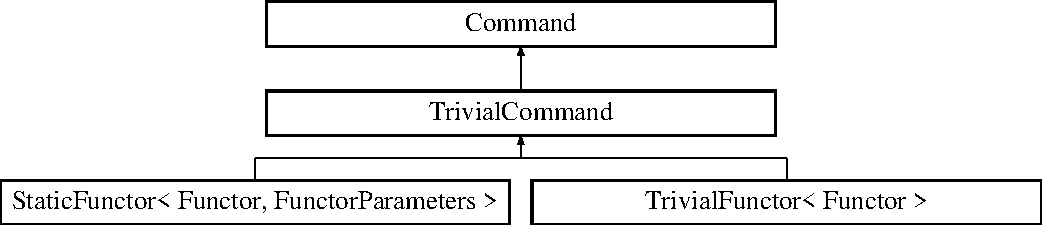
\includegraphics[height=3.000000cm]{class_trivial_command}
\end{center}
\end{figure}
\subsection*{Public Member Functions}
\begin{DoxyCompactItemize}
\item 
\mbox{\Hypertarget{class_trivial_command_aa04f1b1e89d9b70d18abb1979f7a176f}\label{class_trivial_command_aa04f1b1e89d9b70d18abb1979f7a176f}} 
{\bfseries Trivial\+Command} (std\+::string name=\char`\"{}\char`\"{}, std\+::string description=\char`\"{}\char`\"{})
\item 
\mbox{\Hypertarget{class_trivial_command_aac7f01c15634087676f76fdc12a14a79}\label{class_trivial_command_aac7f01c15634087676f76fdc12a14a79}} 
{\bfseries Trivial\+Command} (const \mbox{\hyperlink{class_trivial_command}{Trivial\+Command}} \&copy)=default
\item 
\mbox{\Hypertarget{class_trivial_command_ae2f84a7ac26dc67a55b67dfdc7be54cd}\label{class_trivial_command_ae2f84a7ac26dc67a55b67dfdc7be54cd}} 
{\bfseries Trivial\+Command} (\mbox{\hyperlink{class_trivial_command}{Trivial\+Command}} \&\&move)=default
\item 
\mbox{\Hypertarget{class_trivial_command_a03d7829b8abd891128503a863c1824ff}\label{class_trivial_command_a03d7829b8abd891128503a863c1824ff}} 
\mbox{\hyperlink{class_trivial_command}{Trivial\+Command}} \& {\bfseries operator=} (const \mbox{\hyperlink{class_trivial_command}{Trivial\+Command}} \&rhs)=default
\item 
\mbox{\Hypertarget{class_trivial_command_aa61a3e5fd78d3a2dec6fcf6dcb2e5189}\label{class_trivial_command_aa61a3e5fd78d3a2dec6fcf6dcb2e5189}} 
virtual void {\bfseries operator()} ()=0
\end{DoxyCompactItemize}
\subsection*{Additional Inherited Members}


\subsection{Detailed Description}
Exactly the same as \mbox{\hyperlink{class_command}{Command}}. However, does not support \textquotesingle{}usage\textquotesingle{} nor command arguments. This is used as a wrapper for an invokable to be used in \mbox{\hyperlink{class_engine}{Engine}}. This is an abstract class. To utilise your own Trivial\+Commands, create classes which inherit and override virtual void operator()() to provide your desired functionality. 

The documentation for this class was generated from the following files\+:\begin{DoxyCompactItemize}
\item 
src/command.\+hpp\item 
src/command.\+cpp\end{DoxyCompactItemize}

\hypertarget{class_trivial_functor}{}\section{Trivial\+Functor$<$ Functor $>$ Class Template Reference}
\label{class_trivial_functor}\index{Trivial\+Functor$<$ Functor $>$@{Trivial\+Functor$<$ Functor $>$}}


{\ttfamily \#include $<$command.\+hpp$>$}

Inheritance diagram for Trivial\+Functor$<$ Functor $>$\+:\begin{figure}[H]
\begin{center}
\leavevmode
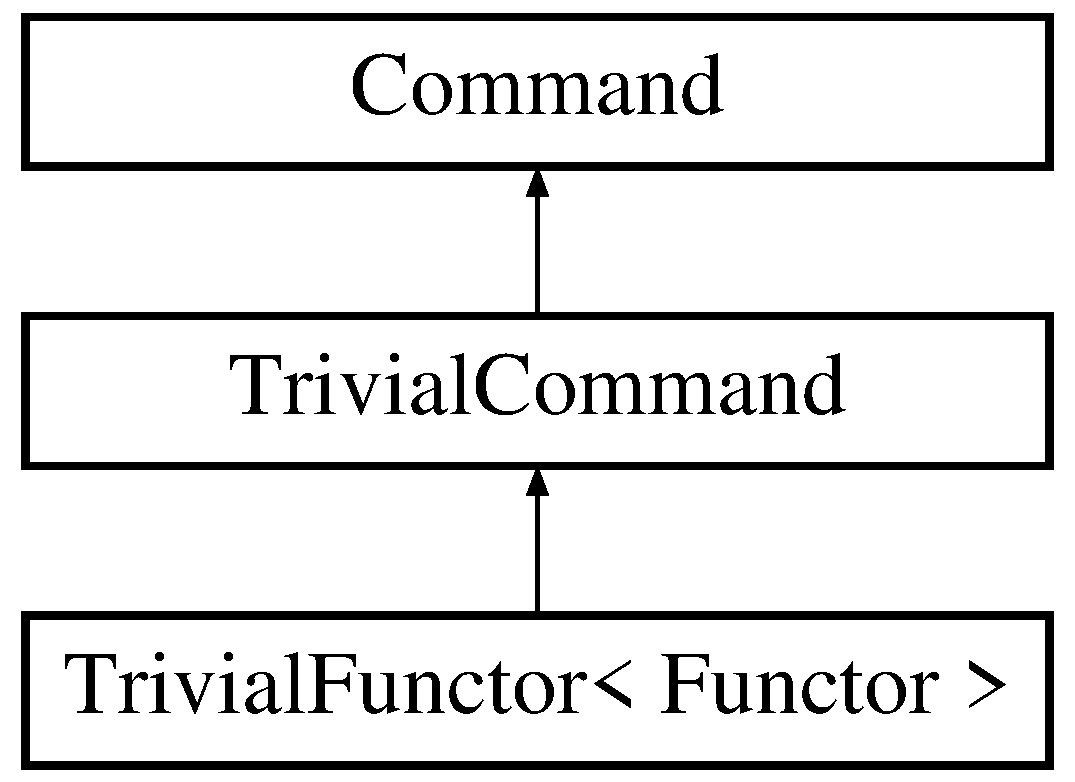
\includegraphics[height=3.000000cm]{class_trivial_functor}
\end{center}
\end{figure}
\subsection*{Public Member Functions}
\begin{DoxyCompactItemize}
\item 
\mbox{\Hypertarget{class_trivial_functor_ab5798bb2ea9fcdb5bf910662ac49c34c}\label{class_trivial_functor_ab5798bb2ea9fcdb5bf910662ac49c34c}} 
{\bfseries Trivial\+Functor} (\mbox{\hyperlink{class_functor}{Functor}} \&\&functor)
\item 
\mbox{\Hypertarget{class_trivial_functor_a5f9b8d18c11a057c2b3e97703262d1e9}\label{class_trivial_functor_a5f9b8d18c11a057c2b3e97703262d1e9}} 
virtual void {\bfseries operator()} () override
\end{DoxyCompactItemize}
\subsection*{Protected Attributes}
\begin{DoxyCompactItemize}
\item 
\mbox{\Hypertarget{class_trivial_functor_a293617a9f9c35365e37237183c7e6fac}\label{class_trivial_functor_a293617a9f9c35365e37237183c7e6fac}} 
\mbox{\hyperlink{class_functor}{Functor}} {\bfseries functor}
\end{DoxyCompactItemize}


\subsection{Detailed Description}
\subsubsection*{template$<$typename Functor$>$\newline
class Trivial\+Functor$<$ Functor $>$}

Wrapper for a trivially-\/invokable object. Trivially-\/invokable objects contain a definition of \textquotesingle{}operator() const\textquotesingle{} taking no arguments. If the functor is not trivially invokable, you must use either a \mbox{\hyperlink{class_static_functor}{Static\+Functor}} or the \mbox{\hyperlink{class_functor}{Functor}} class. 
\begin{DoxyTemplParams}{Template Parameters}
{\em \mbox{\hyperlink{class_functor}{Functor}}} & -\/ \mbox{\hyperlink{class_functor}{Functor}} type, normally an anonymous class (lambda) \\
\hline
\end{DoxyTemplParams}


The documentation for this class was generated from the following files\+:\begin{DoxyCompactItemize}
\item 
src/command.\+hpp\item 
src/command.\+inl\end{DoxyCompactItemize}

\hypertarget{class_uniform}{}\section{Uniform$<$ T $>$ Class Template Reference}
\label{class_uniform}\index{Uniform$<$ T $>$@{Uniform$<$ T $>$}}


{\ttfamily \#include $<$shader.\+hpp$>$}

Inheritance diagram for Uniform$<$ T $>$\+:\begin{figure}[H]
\begin{center}
\leavevmode
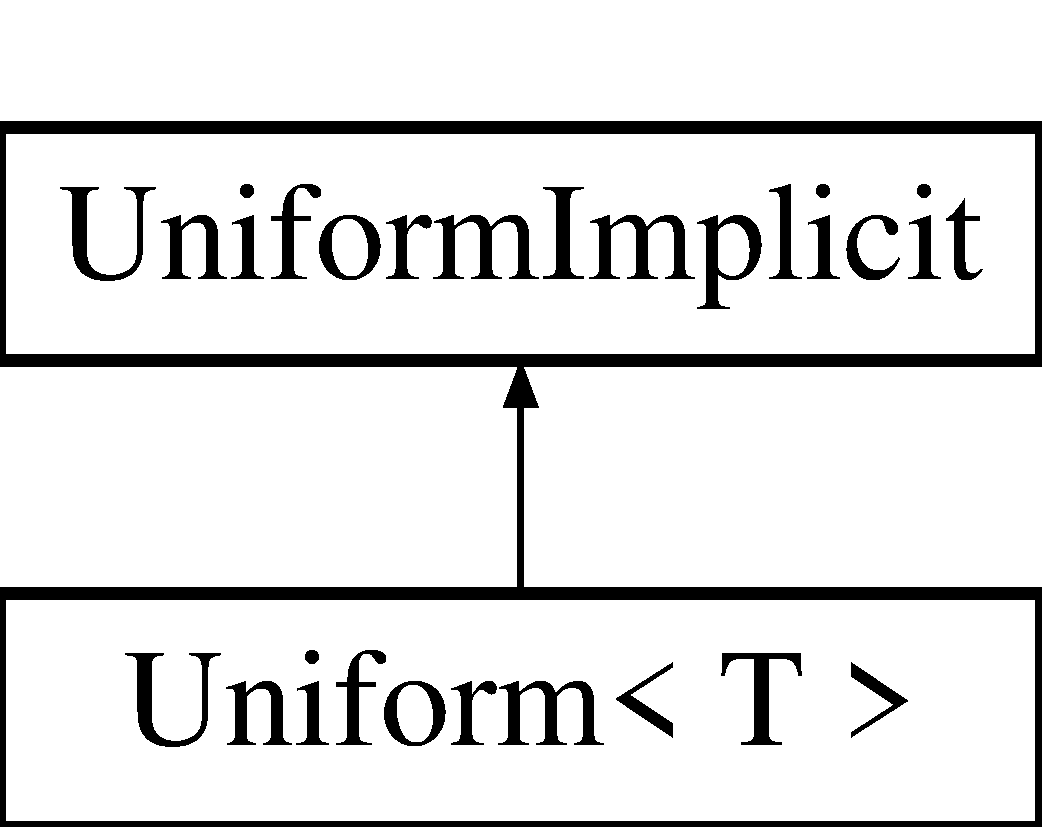
\includegraphics[height=2.000000cm]{class_uniform}
\end{center}
\end{figure}
\subsection*{Public Member Functions}
\begin{DoxyCompactItemize}
\item 
\mbox{\Hypertarget{class_uniform_a3d219b0bb43be48b26bc40c0dc8e3d4f}\label{class_uniform_a3d219b0bb43be48b26bc40c0dc8e3d4f}} 
{\bfseries Uniform} (G\+Luint shader\+\_\+handle, std\+::string uniform\+\_\+location, T value)
\item 
\mbox{\Hypertarget{class_uniform_a1648183f45498b00a7ad72cb2588217c}\label{class_uniform_a1648183f45498b00a7ad72cb2588217c}} 
{\bfseries Uniform} (const \mbox{\hyperlink{class_uniform}{Uniform}}$<$ T $>$ \&copy)=delete
\item 
\mbox{\Hypertarget{class_uniform_a072b528f854a1e9c39af4292b1893821}\label{class_uniform_a072b528f854a1e9c39af4292b1893821}} 
{\bfseries Uniform} (\mbox{\hyperlink{class_uniform}{Uniform}}$<$ T $>$ \&\&move)=default
\item 
\mbox{\Hypertarget{class_uniform_a4018014ae7a377e136ad56baab73ec8b}\label{class_uniform_a4018014ae7a377e136ad56baab73ec8b}} 
G\+Luint {\bfseries get\+\_\+shader\+\_\+handle} () const
\item 
\mbox{\Hypertarget{class_uniform_a5ac04abebea4b8ab2c75e937795ec412}\label{class_uniform_a5ac04abebea4b8ab2c75e937795ec412}} 
virtual std\+::string\+\_\+view {\bfseries get\+\_\+uniform\+\_\+location} () const final
\item 
\mbox{\Hypertarget{class_uniform_a932ed069688bd4086b0b0b7d197c3ee3}\label{class_uniform_a932ed069688bd4086b0b0b7d197c3ee3}} 
const T \& {\bfseries get\+\_\+value} () const
\item 
\mbox{\Hypertarget{class_uniform_abd3def6c98078007579bac6bb5806196}\label{class_uniform_abd3def6c98078007579bac6bb5806196}} 
void {\bfseries set\+\_\+value} (T value)
\item 
\mbox{\Hypertarget{class_uniform_a6089ea0848616549c01c0fde1edaf1c9}\label{class_uniform_a6089ea0848616549c01c0fde1edaf1c9}} 
virtual void {\bfseries push} () const final
\end{DoxyCompactItemize}


\subsection{Detailed Description}
\subsubsection*{template$<$class T$>$\newline
class Uniform$<$ T $>$}

Represent an Open\+GL uniform in C++. Supports the following Topaz/\+C++ primitives\+: bool, int, unsigned int, float, double, Vector2F, Vector3F, Vector4F, \mbox{\hyperlink{class_matrix2x2}{Matrix2x2}}, \mbox{\hyperlink{class_matrix3x3}{Matrix3x3}}, and \mbox{\hyperlink{class_matrix4x4}{Matrix4x4}}. If the template argument is not any of these types, a static assertation will fail in Uniform$<$\+T$>$\+::push and emit a compiler error. 

The documentation for this class was generated from the following files\+:\begin{DoxyCompactItemize}
\item 
src/graphics/shader.\+hpp\item 
src/graphics/shader.\+inl\end{DoxyCompactItemize}

\hypertarget{class_uniform_implicit}{}\section{Uniform\+Implicit Class Reference}
\label{class_uniform_implicit}\index{Uniform\+Implicit@{Uniform\+Implicit}}
Inheritance diagram for Uniform\+Implicit\+:\begin{figure}[H]
\begin{center}
\leavevmode
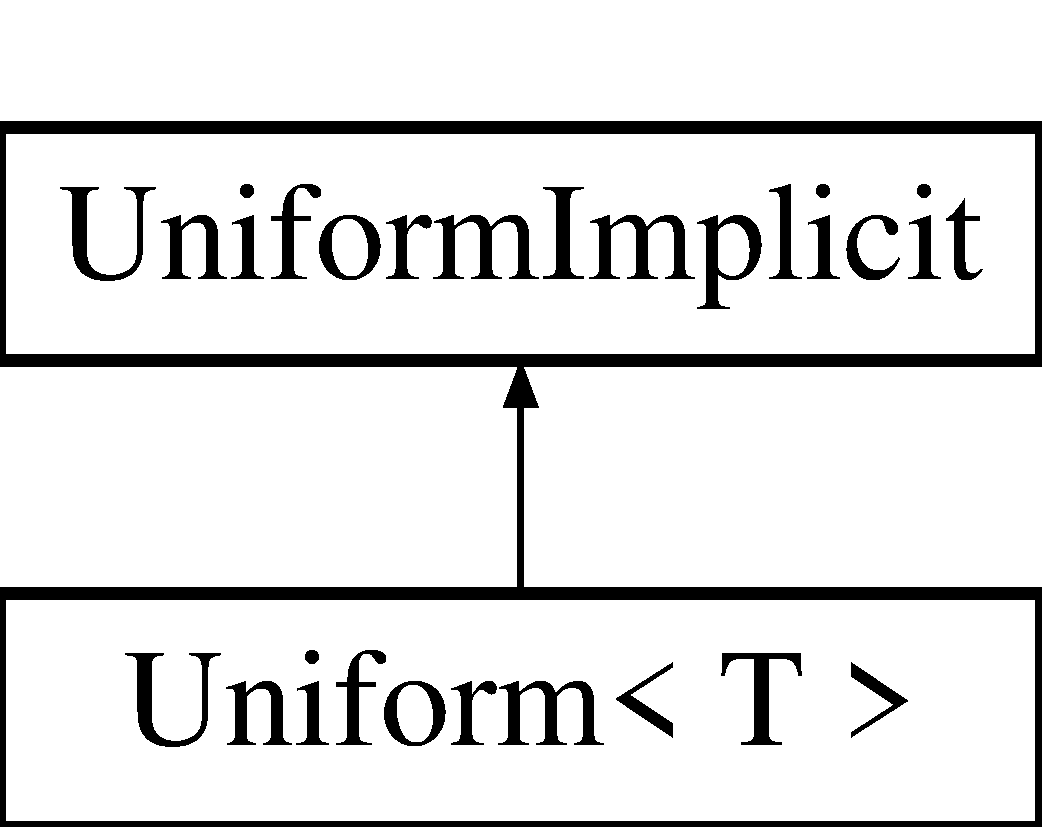
\includegraphics[height=2.000000cm]{class_uniform_implicit}
\end{center}
\end{figure}
\subsection*{Public Member Functions}
\begin{DoxyCompactItemize}
\item 
\mbox{\Hypertarget{class_uniform_implicit_aee430c236fdcb8fffb52e42f8d693e94}\label{class_uniform_implicit_aee430c236fdcb8fffb52e42f8d693e94}} 
virtual G\+Luint {\bfseries get\+\_\+shader\+\_\+handle} () const =0
\item 
\mbox{\Hypertarget{class_uniform_implicit_afe64ca7076103269633a6e0ffbf1a63d}\label{class_uniform_implicit_afe64ca7076103269633a6e0ffbf1a63d}} 
virtual std\+::string\+\_\+view {\bfseries get\+\_\+uniform\+\_\+location} () const =0
\item 
\mbox{\Hypertarget{class_uniform_implicit_ab417a55fb98b7b919f89dc549561475e}\label{class_uniform_implicit_ab417a55fb98b7b919f89dc549561475e}} 
virtual void {\bfseries push} () const =0
\end{DoxyCompactItemize}


The documentation for this class was generated from the following file\+:\begin{DoxyCompactItemize}
\item 
src/graphics/shader.\+hpp\end{DoxyCompactItemize}

\hypertarget{class_vector}{}\section{Vector$<$ N, T $>$ Class Template Reference}
\label{class_vector}\index{Vector$<$ N, T $>$@{Vector$<$ N, T $>$}}


{\ttfamily \#include $<$vector.\+hpp$>$}

\subsection*{Public Member Functions}
\begin{DoxyCompactItemize}
\item 
constexpr \mbox{\hyperlink{class_vector_abae6eb6eff55acb2894297c9f734c2d9}{Vector}} (std\+::array$<$ T, N $>$ data)
\item 
\mbox{\Hypertarget{class_vector_a419b12d187f250ac7fa9a94ec903f210}\label{class_vector_a419b12d187f250ac7fa9a94ec903f210}} 
{\bfseries Vector} (const \mbox{\hyperlink{class_vector}{Vector}}$<$ N, T $>$ \&copy)
\item 
\mbox{\Hypertarget{class_vector_a1a62e62b04841a8a8a68f70f99c8c1b9}\label{class_vector_a1a62e62b04841a8a8a68f70f99c8c1b9}} 
{\bfseries Vector} (\mbox{\hyperlink{class_vector}{Vector}}$<$ N, T $>$ \&\&move)
\item 
\mbox{\Hypertarget{class_vector_a895d481d7672a14c2fe72803cd7c5668}\label{class_vector_a895d481d7672a14c2fe72803cd7c5668}} 
\mbox{\hyperlink{class_vector}{Vector}}$<$ N, T $>$ \& {\bfseries operator=} (const \mbox{\hyperlink{class_vector}{Vector}}$<$ N, T $>$ \&rhs)
\item 
T \mbox{\hyperlink{class_vector_ae8a43ee89f0a311a44711db03c1ddb4b}{length}} (std\+::function$<$ T(T)$>$ sqrt\+\_\+function=std\+::sqrt) const
\end{DoxyCompactItemize}
\subsection*{Public Attributes}
\begin{DoxyCompactItemize}
\item 
\mbox{\Hypertarget{class_vector_a8d06c36075458e4fd7ca17ba171ac549}\label{class_vector_a8d06c36075458e4fd7ca17ba171ac549}} 
std\+::array$<$ T, N $>$ {\bfseries data}
\end{DoxyCompactItemize}


\subsection{Detailed Description}
\subsubsection*{template$<$unsigned int N, typename T$>$\newline
class Vector$<$ N, T $>$}

\mbox{\hyperlink{class_vector}{Vector}} to hold a quantity of some value. It\textquotesingle{}s a glorified array. 
\begin{DoxyTemplParams}{Template Parameters}
{\em N} & -\/ Number of elements \\
\hline
{\em T} & -\/ Type of element \\
\hline
\end{DoxyTemplParams}


\subsection{Constructor \& Destructor Documentation}
\mbox{\Hypertarget{class_vector_abae6eb6eff55acb2894297c9f734c2d9}\label{class_vector_abae6eb6eff55acb2894297c9f734c2d9}} 
\index{Vector@{Vector}!Vector@{Vector}}
\index{Vector@{Vector}!Vector@{Vector}}
\subsubsection{\texorpdfstring{Vector()}{Vector()}}
{\footnotesize\ttfamily template$<$unsigned int N, typename T$>$ \\
constexpr \mbox{\hyperlink{class_vector}{Vector}}$<$ N, T $>$\+::\mbox{\hyperlink{class_vector}{Vector}} (\begin{DoxyParamCaption}\item[{std\+::array$<$ T, N $>$}]{data }\end{DoxyParamCaption})}

Construct a \mbox{\hyperlink{class_vector}{Vector}} directly from an array. 
\begin{DoxyParams}{Parameters}
{\em data} & -\/ The data to be copied into the vector. \\
\hline
\end{DoxyParams}


\subsection{Member Function Documentation}
\mbox{\Hypertarget{class_vector_ae8a43ee89f0a311a44711db03c1ddb4b}\label{class_vector_ae8a43ee89f0a311a44711db03c1ddb4b}} 
\index{Vector@{Vector}!length@{length}}
\index{length@{length}!Vector@{Vector}}
\subsubsection{\texorpdfstring{length()}{length()}}
{\footnotesize\ttfamily template$<$unsigned int N, typename T$>$ \\
T \mbox{\hyperlink{class_vector}{Vector}}$<$ N, T $>$\+::length (\begin{DoxyParamCaption}\item[{std\+::function$<$ T(T)$>$}]{sqrt\+\_\+function = {\ttfamily std\+:\+:sqrt} }\end{DoxyParamCaption}) const}

Return magnitude of the \mbox{\hyperlink{class_vector}{Vector}}. 
\begin{DoxyParams}{Parameters}
{\em sqrt\+\_\+function} & -\/ The function to use to perform a square-\/root on the type T. If none is provided, the default std\+::sqrt will be used. \\
\hline
\end{DoxyParams}
\begin{DoxyReturn}{Returns}
-\/ Magnitude of the \mbox{\hyperlink{class_vector}{Vector}}. 
\end{DoxyReturn}


The documentation for this class was generated from the following files\+:\begin{DoxyCompactItemize}
\item 
src/vector.\+hpp\item 
src/vector.\+inl\end{DoxyCompactItemize}

\hypertarget{class_vector2}{}\section{Vector2$<$ T $>$ Class Template Reference}
\label{class_vector2}\index{Vector2$<$ T $>$@{Vector2$<$ T $>$}}


{\ttfamily \#include $<$vector.\+hpp$>$}

Inheritance diagram for Vector2$<$ T $>$\+:\begin{figure}[H]
\begin{center}
\leavevmode
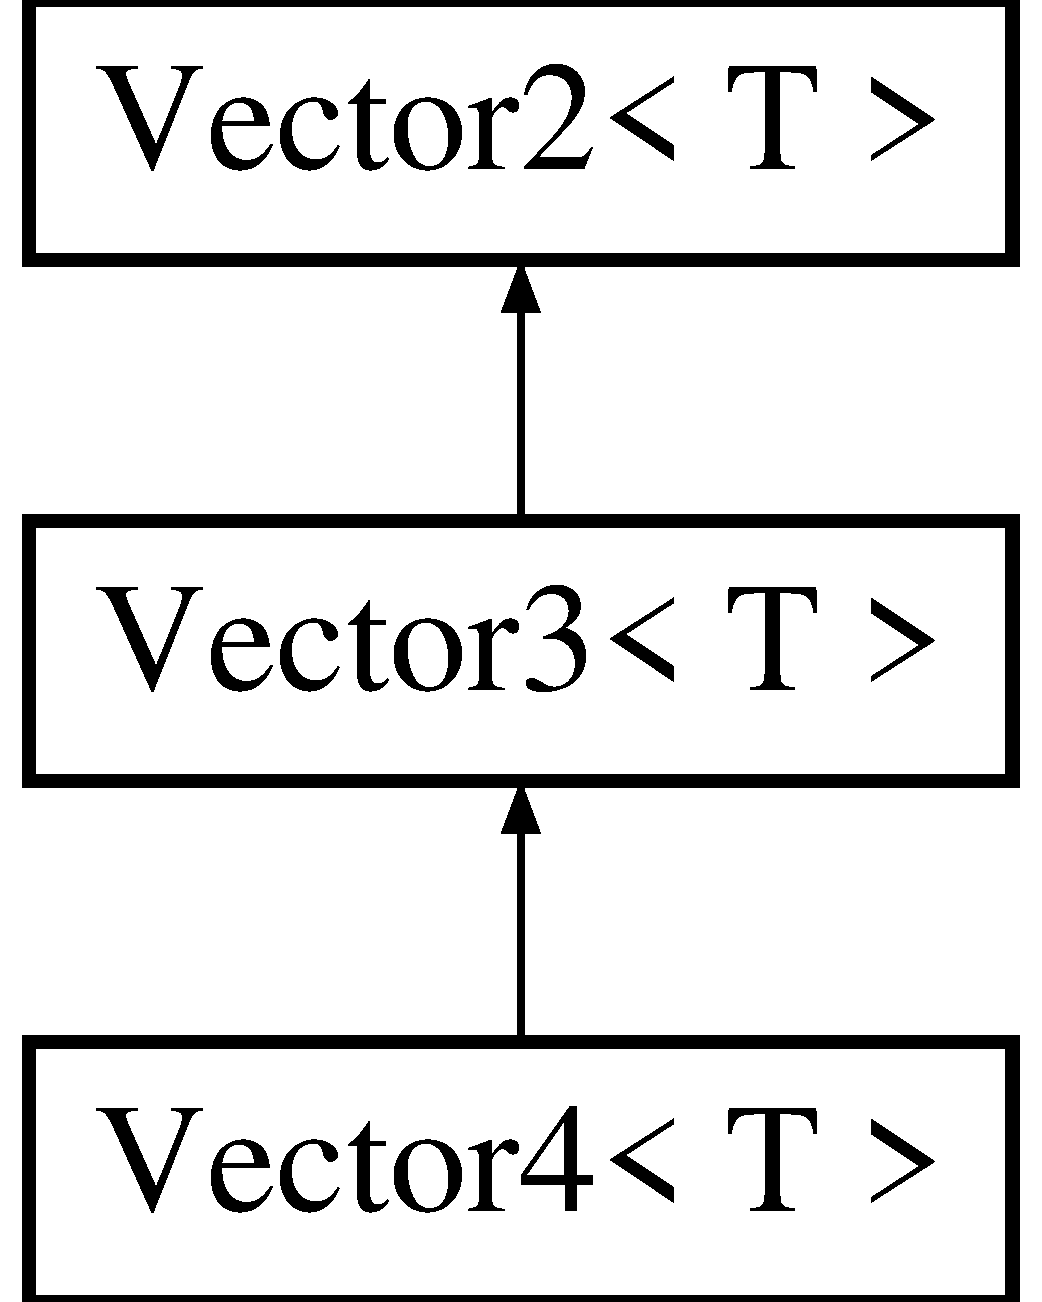
\includegraphics[height=3.000000cm]{class_vector2}
\end{center}
\end{figure}
\subsection*{Public Member Functions}
\begin{DoxyCompactItemize}
\item 
\mbox{\Hypertarget{class_vector2_aabb780b39b3fd9353d95cc11f3d626c2}\label{class_vector2_aabb780b39b3fd9353d95cc11f3d626c2}} 
{\bfseries Vector2} (T x=T(), T y=T())
\item 
\mbox{\Hypertarget{class_vector2_ae611e87470765c3e8ed27bdc8971d0ce}\label{class_vector2_ae611e87470765c3e8ed27bdc8971d0ce}} 
constexpr {\bfseries Vector2} (const std\+::array$<$ T, 2 $>$ \&data)
\item 
\mbox{\Hypertarget{class_vector2_a663fa4a2709dd5666eff6b3cf205e7b0}\label{class_vector2_a663fa4a2709dd5666eff6b3cf205e7b0}} 
{\bfseries Vector2} (const \mbox{\hyperlink{class_vector2}{Vector2}}$<$ T $>$ \&copy)=default
\item 
\mbox{\Hypertarget{class_vector2_ab5412c7d71fe6364dcf3c5eb1e88198a}\label{class_vector2_ab5412c7d71fe6364dcf3c5eb1e88198a}} 
{\bfseries Vector2} (\mbox{\hyperlink{class_vector2}{Vector2}}$<$ T $>$ \&\&move)=default
\item 
\mbox{\Hypertarget{class_vector2_ad0c9d983620766819a289bdf958f71d4}\label{class_vector2_ad0c9d983620766819a289bdf958f71d4}} 
\mbox{\hyperlink{class_vector2}{Vector2}}$<$ T $>$ \& {\bfseries operator=} (const \mbox{\hyperlink{class_vector2}{Vector2}}$<$ T $>$ \&rhs)=default
\item 
\mbox{\Hypertarget{class_vector2_ab4c2e1a3fe9216e506e3ab60c02348b2}\label{class_vector2_ab4c2e1a3fe9216e506e3ab60c02348b2}} 
\mbox{\hyperlink{struct_vector2_p_o_d}{Vector2\+P\+OD}} {\bfseries to\+\_\+raw} () const
\item 
\mbox{\Hypertarget{class_vector2_a784391c74b4bd821fc4a6277170c1263}\label{class_vector2_a784391c74b4bd821fc4a6277170c1263}} 
T {\bfseries length} () const
\item 
\mbox{\Hypertarget{class_vector2_a9f7a1b36270fa93b51546d2b29228e39}\label{class_vector2_a9f7a1b36270fa93b51546d2b29228e39}} 
T {\bfseries dot} (const \mbox{\hyperlink{class_vector2}{Vector2}}$<$ T $>$ \&rhs) const
\item 
\mbox{\Hypertarget{class_vector2_aa21618ee0b6e9684da1a5b2d7c8ad3d4}\label{class_vector2_aa21618ee0b6e9684da1a5b2d7c8ad3d4}} 
\mbox{\hyperlink{class_vector2}{Vector2}}$<$ T $>$ {\bfseries normalised} () const
\item 
\mbox{\Hypertarget{class_vector2_af608a3b5bb42148c2260fb0ba9cf0950}\label{class_vector2_af608a3b5bb42148c2260fb0ba9cf0950}} 
\mbox{\hyperlink{class_vector2}{Vector2}}$<$ T $>$ {\bfseries operator+} (const \mbox{\hyperlink{class_vector2}{Vector2}}$<$ T $>$ \&rhs) const
\item 
\mbox{\Hypertarget{class_vector2_ab79812a53ba6238fdcaef73cb22fcbb3}\label{class_vector2_ab79812a53ba6238fdcaef73cb22fcbb3}} 
\mbox{\hyperlink{class_vector2}{Vector2}}$<$ T $>$ {\bfseries operator-\/} (const \mbox{\hyperlink{class_vector2}{Vector2}}$<$ T $>$ \&rhs) const
\item 
\mbox{\Hypertarget{class_vector2_a6b89b2f334240f06480bc55fce6c2a5a}\label{class_vector2_a6b89b2f334240f06480bc55fce6c2a5a}} 
\mbox{\hyperlink{class_vector2}{Vector2}}$<$ T $>$ {\bfseries operator$\ast$} (T scalar) const
\item 
\mbox{\Hypertarget{class_vector2_aae901abf0c2c7f0c772d8cb69213f628}\label{class_vector2_aae901abf0c2c7f0c772d8cb69213f628}} 
\mbox{\hyperlink{class_vector2}{Vector2}}$<$ T $>$ {\bfseries operator/} (T scalar) const
\item 
\mbox{\Hypertarget{class_vector2_a198ab8bb7f0e0be8905869ccc5b2bf0e}\label{class_vector2_a198ab8bb7f0e0be8905869ccc5b2bf0e}} 
\mbox{\hyperlink{class_vector2}{Vector2}}$<$ T $>$ \& {\bfseries operator+=} (const \mbox{\hyperlink{class_vector2}{Vector2}}$<$ T $>$ \&rhs)
\item 
\mbox{\Hypertarget{class_vector2_a1722e051fa3c354749c2c4c5c14b9c8e}\label{class_vector2_a1722e051fa3c354749c2c4c5c14b9c8e}} 
\mbox{\hyperlink{class_vector2}{Vector2}}$<$ T $>$ \& {\bfseries operator-\/=} (const \mbox{\hyperlink{class_vector2}{Vector2}}$<$ T $>$ \&rhs)
\item 
\mbox{\Hypertarget{class_vector2_ac310f14122b41cbbbb3d4eac98c81f00}\label{class_vector2_ac310f14122b41cbbbb3d4eac98c81f00}} 
\mbox{\hyperlink{class_vector2}{Vector2}}$<$ T $>$ \& {\bfseries operator$\ast$=} (T scalar)
\item 
\mbox{\Hypertarget{class_vector2_a9e79272d8b7b39e8d8eafa6f4cbad04e}\label{class_vector2_a9e79272d8b7b39e8d8eafa6f4cbad04e}} 
\mbox{\hyperlink{class_vector2}{Vector2}}$<$ T $>$ \& {\bfseries operator/=} (T scalar)
\item 
\mbox{\Hypertarget{class_vector2_abeb4df28fbd42c319b3e5529a1805e90}\label{class_vector2_abeb4df28fbd42c319b3e5529a1805e90}} 
bool {\bfseries operator$<$} (const \mbox{\hyperlink{class_vector2}{Vector2}}$<$ T $>$ \&rhs) const
\item 
\mbox{\Hypertarget{class_vector2_ac550f020f264f8a8058ad3c623c60d40}\label{class_vector2_ac550f020f264f8a8058ad3c623c60d40}} 
bool {\bfseries operator$>$} (const \mbox{\hyperlink{class_vector2}{Vector2}}$<$ T $>$ \&rhs) const
\item 
\mbox{\Hypertarget{class_vector2_a0a798a144b107a4a7964da13c1ada290}\label{class_vector2_a0a798a144b107a4a7964da13c1ada290}} 
bool {\bfseries operator$<$=} (const \mbox{\hyperlink{class_vector2}{Vector2}}$<$ T $>$ \&rhs) const
\item 
\mbox{\Hypertarget{class_vector2_aad131ea8361750d0fd577c268ed45cc6}\label{class_vector2_aad131ea8361750d0fd577c268ed45cc6}} 
bool {\bfseries operator$>$=} (const \mbox{\hyperlink{class_vector2}{Vector2}}$<$ T $>$ \&rhs) const
\item 
\mbox{\Hypertarget{class_vector2_a45c07c01d5704a8f7e9b55077034e4f8}\label{class_vector2_a45c07c01d5704a8f7e9b55077034e4f8}} 
bool {\bfseries operator==} (const \mbox{\hyperlink{class_vector2}{Vector2}}$<$ T $>$ \&rhs) const
\item 
\mbox{\Hypertarget{class_vector2_a318be8911fa2fbb1887f95196d26c6e8}\label{class_vector2_a318be8911fa2fbb1887f95196d26c6e8}} 
\mbox{\hyperlink{class_vector2}{Vector2}}$<$ T $>$ {\bfseries xy} () const
\item 
\mbox{\Hypertarget{class_vector2_a45bce734de6f2bc8fc9f0ca6a8bad7a1}\label{class_vector2_a45bce734de6f2bc8fc9f0ca6a8bad7a1}} 
\mbox{\hyperlink{class_vector2}{Vector2}}$<$ T $>$ {\bfseries yx} () const
\end{DoxyCompactItemize}
\subsection*{Public Attributes}
\begin{DoxyCompactItemize}
\item 
\mbox{\Hypertarget{class_vector2_a78fa1f2ed5e261c7fbeb8f3536a1ee34}\label{class_vector2_a78fa1f2ed5e261c7fbeb8f3536a1ee34}} 
T {\bfseries x}
\item 
\mbox{\Hypertarget{class_vector2_a6cfed8355591aa269f4dba43bd806ef9}\label{class_vector2_a6cfed8355591aa269f4dba43bd806ef9}} 
T {\bfseries y}
\end{DoxyCompactItemize}


\subsection{Detailed Description}
\subsubsection*{template$<$typename T$>$\newline
class Vector2$<$ T $>$}

Tuple of two arguments of type T. Similar to an std\+::tuple$<$\+T, T$>$ but contains useful mathematical functions in addition, such as cross-\/products. 
\begin{DoxyTemplParams}{Template Parameters}
{\em T} & -\/ The type of which to store a pair of. \\
\hline
\end{DoxyTemplParams}


The documentation for this class was generated from the following files\+:\begin{DoxyCompactItemize}
\item 
src/vector.\+hpp\item 
src/vector.\+inl\end{DoxyCompactItemize}

\hypertarget{struct_vector2_p_o_d}{}\section{Vector2\+P\+OD Struct Reference}
\label{struct_vector2_p_o_d}\index{Vector2\+P\+OD@{Vector2\+P\+OD}}


{\ttfamily \#include $<$vector.\+hpp$>$}

\subsection*{Public Attributes}
\begin{DoxyCompactItemize}
\item 
\mbox{\Hypertarget{struct_vector2_p_o_d_aae469724c8da4468de3ac9415c75465e}\label{struct_vector2_p_o_d_aae469724c8da4468de3ac9415c75465e}} 
float {\bfseries x}
\item 
\mbox{\Hypertarget{struct_vector2_p_o_d_a8ed0fe76a28039ddae57d8bda8bf2970}\label{struct_vector2_p_o_d_a8ed0fe76a28039ddae57d8bda8bf2970}} 
float {\bfseries y}
\end{DoxyCompactItemize}


\subsection{Detailed Description}
C-\/style P\+OD struct for a Vector2F 

The documentation for this struct was generated from the following file\+:\begin{DoxyCompactItemize}
\item 
src/vector.\+hpp\end{DoxyCompactItemize}

\hypertarget{class_vector3}{}\section{Vector3$<$ T $>$ Class Template Reference}
\label{class_vector3}\index{Vector3$<$ T $>$@{Vector3$<$ T $>$}}


{\ttfamily \#include $<$vector.\+hpp$>$}

Inheritance diagram for Vector3$<$ T $>$\+:\begin{figure}[H]
\begin{center}
\leavevmode
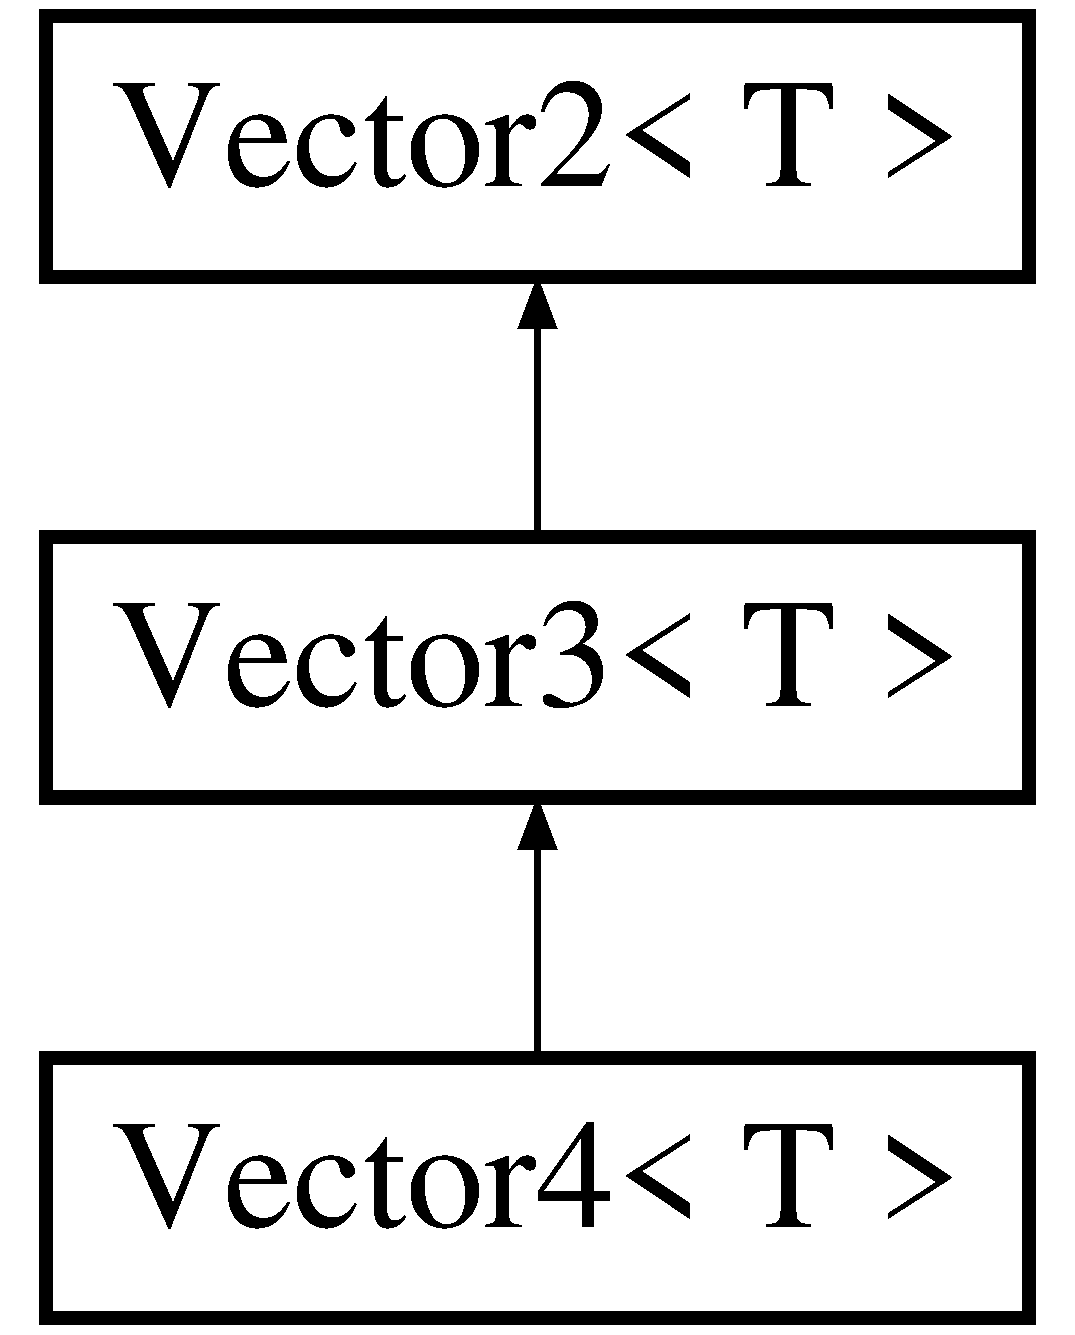
\includegraphics[height=3.000000cm]{class_vector3}
\end{center}
\end{figure}
\subsection*{Public Member Functions}
\begin{DoxyCompactItemize}
\item 
\mbox{\Hypertarget{class_vector3_adbe669edb8e99e52f2977d90216240d6}\label{class_vector3_adbe669edb8e99e52f2977d90216240d6}} 
{\bfseries Vector3} (T x=T(), T y=T(), T z=T())
\item 
\mbox{\Hypertarget{class_vector3_afcc8c0d5ab04576a5d1dac5cfe26ac5a}\label{class_vector3_afcc8c0d5ab04576a5d1dac5cfe26ac5a}} 
{\bfseries Vector3} (\mbox{\hyperlink{class_vector2}{Vector2}}$<$ T $>$ xy, T z)
\item 
\mbox{\Hypertarget{class_vector3_a418527eee55cb85c7482d1e381f1034e}\label{class_vector3_a418527eee55cb85c7482d1e381f1034e}} 
{\bfseries Vector3} (T x, \mbox{\hyperlink{class_vector2}{Vector2}}$<$ T $>$ yz)
\item 
\mbox{\Hypertarget{class_vector3_a071a8ad60a3a8ab6e07b868c5c5fd617}\label{class_vector3_a071a8ad60a3a8ab6e07b868c5c5fd617}} 
constexpr {\bfseries Vector3} (const std\+::array$<$ T, 3 $>$ \&data)
\item 
\mbox{\Hypertarget{class_vector3_a0f1bc2fd756831c7c76cfb53818cd4b9}\label{class_vector3_a0f1bc2fd756831c7c76cfb53818cd4b9}} 
{\bfseries Vector3} (const \mbox{\hyperlink{class_vector3}{Vector3}}$<$ T $>$ \&copy)=default
\item 
\mbox{\Hypertarget{class_vector3_acf8f012882baca43b4c45f14dab5fae6}\label{class_vector3_acf8f012882baca43b4c45f14dab5fae6}} 
{\bfseries Vector3} (\mbox{\hyperlink{class_vector3}{Vector3}}$<$ T $>$ \&\&move)=default
\item 
\mbox{\Hypertarget{class_vector3_a6c79f9f930582d7368e025e771ae7636}\label{class_vector3_a6c79f9f930582d7368e025e771ae7636}} 
\mbox{\hyperlink{class_vector3}{Vector3}}$<$ T $>$ \& {\bfseries operator=} (const \mbox{\hyperlink{class_vector3}{Vector3}}$<$ T $>$ \&rhs)=default
\item 
\mbox{\Hypertarget{class_vector3_a9bc4a07b903235d5a0c81eeb75e856e0}\label{class_vector3_a9bc4a07b903235d5a0c81eeb75e856e0}} 
\mbox{\hyperlink{struct_vector3_p_o_d}{Vector3\+P\+OD}} {\bfseries to\+\_\+raw} () const
\item 
\mbox{\Hypertarget{class_vector3_aa5177b38edaae3717bc94443946345d0}\label{class_vector3_aa5177b38edaae3717bc94443946345d0}} 
T {\bfseries length} () const
\item 
\mbox{\Hypertarget{class_vector3_abf12b7769b13982490e594877236abe1}\label{class_vector3_abf12b7769b13982490e594877236abe1}} 
T {\bfseries dot} (const \mbox{\hyperlink{class_vector3}{Vector3}}$<$ T $>$ \&rhs) const
\item 
\mbox{\Hypertarget{class_vector3_a55d165924a9c4c4fb29aba342259450f}\label{class_vector3_a55d165924a9c4c4fb29aba342259450f}} 
\mbox{\hyperlink{class_vector3}{Vector3}}$<$ T $>$ {\bfseries cross} (const \mbox{\hyperlink{class_vector3}{Vector3}}$<$ T $>$ \&rhs) const
\item 
\mbox{\Hypertarget{class_vector3_a527c54e392f3aa4b942df2eb7aa3b38b}\label{class_vector3_a527c54e392f3aa4b942df2eb7aa3b38b}} 
\mbox{\hyperlink{class_vector3}{Vector3}}$<$ T $>$ {\bfseries normalised} () const
\item 
\mbox{\Hypertarget{class_vector3_ae773f6324d5ee80b042632297e573400}\label{class_vector3_ae773f6324d5ee80b042632297e573400}} 
\mbox{\hyperlink{class_vector3}{Vector3}}$<$ T $>$ {\bfseries operator+} (const \mbox{\hyperlink{class_vector3}{Vector3}}$<$ T $>$ \&rhs) const
\item 
\mbox{\Hypertarget{class_vector3_a385caaf9d5ce60bc720b8304d9c98937}\label{class_vector3_a385caaf9d5ce60bc720b8304d9c98937}} 
\mbox{\hyperlink{class_vector3}{Vector3}}$<$ T $>$ {\bfseries operator-\/} (const \mbox{\hyperlink{class_vector3}{Vector3}}$<$ T $>$ \&rhs) const
\item 
\mbox{\Hypertarget{class_vector3_af1a6bd4542b3cb1d78fb90b81f9b3763}\label{class_vector3_af1a6bd4542b3cb1d78fb90b81f9b3763}} 
\mbox{\hyperlink{class_vector3}{Vector3}}$<$ T $>$ {\bfseries operator$\ast$} (T scalar) const
\item 
\mbox{\Hypertarget{class_vector3_a50099461c7eeb5471b022918de5c86c3}\label{class_vector3_a50099461c7eeb5471b022918de5c86c3}} 
\mbox{\hyperlink{class_vector3}{Vector3}}$<$ T $>$ {\bfseries operator/} (T scalar) const
\item 
\mbox{\Hypertarget{class_vector3_a46410fa08aa469fe979bc29601ee18f0}\label{class_vector3_a46410fa08aa469fe979bc29601ee18f0}} 
\mbox{\hyperlink{class_vector3}{Vector3}}$<$ T $>$ \& {\bfseries operator+=} (const \mbox{\hyperlink{class_vector3}{Vector3}}$<$ T $>$ \&rhs)
\item 
\mbox{\Hypertarget{class_vector3_a57ae63fe916c0042a46545780b23c05e}\label{class_vector3_a57ae63fe916c0042a46545780b23c05e}} 
\mbox{\hyperlink{class_vector3}{Vector3}}$<$ T $>$ \& {\bfseries operator-\/=} (const \mbox{\hyperlink{class_vector3}{Vector3}}$<$ T $>$ \&rhs)
\item 
\mbox{\Hypertarget{class_vector3_af44f1cfdedf62a46e803d838ed6640ad}\label{class_vector3_af44f1cfdedf62a46e803d838ed6640ad}} 
\mbox{\hyperlink{class_vector3}{Vector3}}$<$ T $>$ \& {\bfseries operator$\ast$=} (T scalar)
\item 
\mbox{\Hypertarget{class_vector3_a1fa0486589a5b3e0110902bb5ffa6d71}\label{class_vector3_a1fa0486589a5b3e0110902bb5ffa6d71}} 
\mbox{\hyperlink{class_vector3}{Vector3}}$<$ T $>$ \& {\bfseries operator/=} (T scalar)
\item 
\mbox{\Hypertarget{class_vector3_ae62b088c2abf8ad6620d83565812ad60}\label{class_vector3_ae62b088c2abf8ad6620d83565812ad60}} 
bool {\bfseries operator$<$} (const \mbox{\hyperlink{class_vector3}{Vector3}}$<$ T $>$ \&rhs) const
\item 
\mbox{\Hypertarget{class_vector3_a87afbd96a97adff42c58bde870af47c4}\label{class_vector3_a87afbd96a97adff42c58bde870af47c4}} 
bool {\bfseries operator$>$} (const \mbox{\hyperlink{class_vector3}{Vector3}}$<$ T $>$ \&rhs) const
\item 
\mbox{\Hypertarget{class_vector3_ac7cd56bfa861b5f99b3891f220f86d44}\label{class_vector3_ac7cd56bfa861b5f99b3891f220f86d44}} 
bool {\bfseries operator$<$=} (const \mbox{\hyperlink{class_vector3}{Vector3}}$<$ T $>$ \&rhs) const
\item 
\mbox{\Hypertarget{class_vector3_a9c0fd2c3f2cce9af0711f9ea40bff86a}\label{class_vector3_a9c0fd2c3f2cce9af0711f9ea40bff86a}} 
bool {\bfseries operator$>$=} (const \mbox{\hyperlink{class_vector3}{Vector3}}$<$ T $>$ \&rhs) const
\item 
\mbox{\Hypertarget{class_vector3_a4206accf1c00e63b0181a56a32ba3c01}\label{class_vector3_a4206accf1c00e63b0181a56a32ba3c01}} 
bool {\bfseries operator==} (const \mbox{\hyperlink{class_vector3}{Vector3}}$<$ T $>$ \&rhs) const
\item 
\mbox{\Hypertarget{class_vector3_a19844da39de7a26862856c7d12a009ca}\label{class_vector3_a19844da39de7a26862856c7d12a009ca}} 
\mbox{\hyperlink{class_vector3}{Vector3}}$<$ T $>$ {\bfseries xyz} () const
\item 
\mbox{\Hypertarget{class_vector3_a890a30bec732a65aaae386eb21d393df}\label{class_vector3_a890a30bec732a65aaae386eb21d393df}} 
\mbox{\hyperlink{class_vector3}{Vector3}}$<$ T $>$ {\bfseries xzy} () const
\item 
\mbox{\Hypertarget{class_vector3_ab026847d50c092c8ccf5c5314edca3db}\label{class_vector3_ab026847d50c092c8ccf5c5314edca3db}} 
\mbox{\hyperlink{class_vector3}{Vector3}}$<$ T $>$ {\bfseries yxz} () const
\item 
\mbox{\Hypertarget{class_vector3_a678d9ca488ba19d592965d0094bd685f}\label{class_vector3_a678d9ca488ba19d592965d0094bd685f}} 
\mbox{\hyperlink{class_vector3}{Vector3}}$<$ T $>$ {\bfseries yzx} () const
\item 
\mbox{\Hypertarget{class_vector3_a325fdcf29fb440716dcb22583822e3b4}\label{class_vector3_a325fdcf29fb440716dcb22583822e3b4}} 
\mbox{\hyperlink{class_vector3}{Vector3}}$<$ T $>$ {\bfseries zxy} () const
\item 
\mbox{\Hypertarget{class_vector3_a43ee17c0dffc0290b18db9464c802be9}\label{class_vector3_a43ee17c0dffc0290b18db9464c802be9}} 
\mbox{\hyperlink{class_vector3}{Vector3}}$<$ T $>$ {\bfseries zyx} () const
\end{DoxyCompactItemize}
\subsection*{Public Attributes}
\begin{DoxyCompactItemize}
\item 
\mbox{\Hypertarget{class_vector3_ab3e7f5401dd6e951978bfa746809f74f}\label{class_vector3_ab3e7f5401dd6e951978bfa746809f74f}} 
T {\bfseries z}
\end{DoxyCompactItemize}


\subsection{Detailed Description}
\subsubsection*{template$<$typename T$>$\newline
class Vector3$<$ T $>$}

Tuple of three arguments of type T. Similar to an std\+::tuple$<$\+T, T, T$>$ but contains useful mathematical functions in addition, such as cross-\/products. 
\begin{DoxyTemplParams}{Template Parameters}
{\em T} & -\/ The type of which to store a trio of. \\
\hline
\end{DoxyTemplParams}


The documentation for this class was generated from the following files\+:\begin{DoxyCompactItemize}
\item 
src/vector.\+hpp\item 
src/vector.\+inl\end{DoxyCompactItemize}

\hypertarget{struct_vector3_p_o_d}{}\section{Vector3\+P\+OD Struct Reference}
\label{struct_vector3_p_o_d}\index{Vector3\+P\+OD@{Vector3\+P\+OD}}


{\ttfamily \#include $<$vector.\+hpp$>$}

\subsection*{Public Attributes}
\begin{DoxyCompactItemize}
\item 
\mbox{\Hypertarget{struct_vector3_p_o_d_a20697d084c23e3126914c6a10c300073}\label{struct_vector3_p_o_d_a20697d084c23e3126914c6a10c300073}} 
float {\bfseries x}
\item 
\mbox{\Hypertarget{struct_vector3_p_o_d_a00596acd41b53ab2b5a2667239d81083}\label{struct_vector3_p_o_d_a00596acd41b53ab2b5a2667239d81083}} 
float {\bfseries y}
\item 
\mbox{\Hypertarget{struct_vector3_p_o_d_a7fd1670144f56971ad09dc1887fb741b}\label{struct_vector3_p_o_d_a7fd1670144f56971ad09dc1887fb741b}} 
float {\bfseries z}
\end{DoxyCompactItemize}


\subsection{Detailed Description}
Plain-\/\+Old-\/\+Data structure of a Vector2F. 

The documentation for this struct was generated from the following file\+:\begin{DoxyCompactItemize}
\item 
src/vector.\+hpp\end{DoxyCompactItemize}

\hypertarget{class_vector4}{}\section{Vector4$<$ T $>$ Class Template Reference}
\label{class_vector4}\index{Vector4$<$ T $>$@{Vector4$<$ T $>$}}


{\ttfamily \#include $<$vector.\+hpp$>$}

Inheritance diagram for Vector4$<$ T $>$\+:\begin{figure}[H]
\begin{center}
\leavevmode
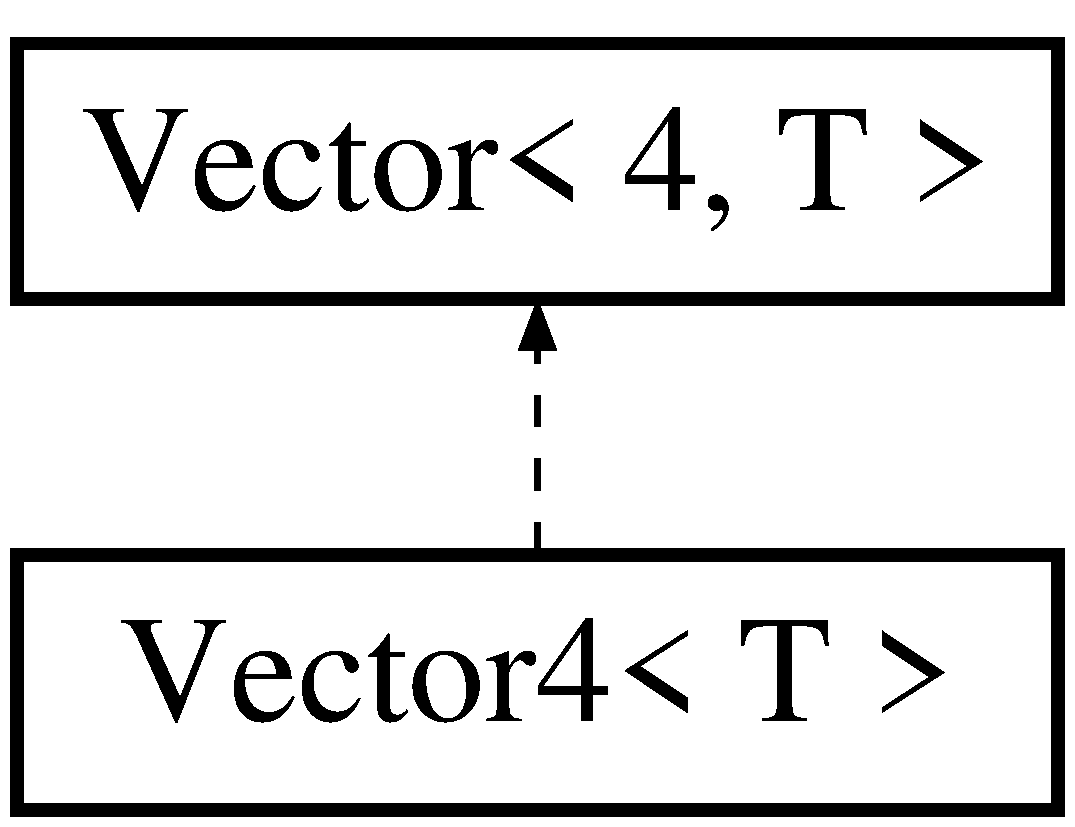
\includegraphics[height=2.000000cm]{class_vector4}
\end{center}
\end{figure}
\subsection*{Public Member Functions}
\begin{DoxyCompactItemize}
\item 
constexpr \mbox{\hyperlink{class_vector4_a31fd25d0c9ad1a2cecd77ea11449b1df}{Vector4}} (T x=T(), T y=T(), T z=T(), T w=T())
\item 
constexpr \mbox{\hyperlink{class_vector4_aaf5bba42bd8e0326baf0ae5f4231178f}{Vector4}} (\mbox{\hyperlink{class_vector3}{Vector3}}$<$ T $>$ \mbox{\hyperlink{class_vector4_a64bc2c65683c50be01c8646487d4d5b2}{xyz}}, T w)
\item 
constexpr \mbox{\hyperlink{class_vector4_a91352d9e5a2063fdc15234ceb3492dc4}{Vector4}} (T x, \mbox{\hyperlink{class_vector3}{Vector3}}$<$ T $>$ yzw)
\item 
constexpr \mbox{\hyperlink{class_vector4_a350701fc93b120a693efc7ab313f0a8a}{Vector4}} (\mbox{\hyperlink{class_vector2}{Vector2}}$<$ T $>$ \mbox{\hyperlink{class_vector4_aca433dfa3d0e963899d6a3916fda347a}{xy}}, \mbox{\hyperlink{class_vector2}{Vector2}}$<$ T $>$ zw)
\item 
constexpr \mbox{\hyperlink{class_vector4_a2503315a6418e38bf423c9fb7b33eec3}{Vector4}} (const std\+::array$<$ T, 4 $>$ \&data)
\item 
\mbox{\Hypertarget{class_vector4_a1095f023acf24ec6f86301378f2a07b9}\label{class_vector4_a1095f023acf24ec6f86301378f2a07b9}} 
{\bfseries Vector4} (const \mbox{\hyperlink{class_vector4}{Vector4}}$<$ T $>$ \&copy)
\item 
\mbox{\Hypertarget{class_vector4_a8e5281eeaaa1b01944d37ca499582cb8}\label{class_vector4_a8e5281eeaaa1b01944d37ca499582cb8}} 
{\bfseries Vector4} (\mbox{\hyperlink{class_vector4}{Vector4}}$<$ T $>$ \&\&move)
\item 
\mbox{\Hypertarget{class_vector4_ac509e5d08d3222ebb06922ca5467ae02}\label{class_vector4_ac509e5d08d3222ebb06922ca5467ae02}} 
\mbox{\hyperlink{class_vector4}{Vector4}}$<$ T $>$ \& {\bfseries operator=} (const \mbox{\hyperlink{class_vector4}{Vector4}}$<$ T $>$ \&rhs)
\item 
\mbox{\hyperlink{struct_vector4_p_o_d}{Vector4\+P\+OD}} \mbox{\hyperlink{class_vector4_a4fea99cf190d3d29f9aaa36acd07a49a}{to\+\_\+raw}} () const
\item 
T \mbox{\hyperlink{class_vector4_a1c8ab62fe32713c21353d71a1b23b0f2}{length}} () const
\item 
T \mbox{\hyperlink{class_vector4_ae9d1720458cdff4084f2f20dadbc0dd7}{dot}} (\mbox{\hyperlink{class_vector4}{Vector4}}$<$ T $>$ rhs) const
\item 
\mbox{\hyperlink{class_vector4}{Vector4}}$<$ T $>$ \mbox{\hyperlink{class_vector4_ab03ee378cc4b82bcb2429ca4fe7fe53b}{normalised}} () const
\item 
\mbox{\hyperlink{class_vector4}{Vector4}}$<$ T $>$ \mbox{\hyperlink{class_vector4_a2a7fd8018536c8e7c61b8ee3975609f9}{operator+}} (const \mbox{\hyperlink{class_vector4}{Vector4}}$<$ T $>$ \&rhs) const
\item 
\mbox{\hyperlink{class_vector4}{Vector4}}$<$ T $>$ \mbox{\hyperlink{class_vector4_a41cb957697e0e937e0f7f4a5d459575a}{operator-\/}} (const \mbox{\hyperlink{class_vector4}{Vector4}}$<$ T $>$ \&rhs) const
\item 
\mbox{\hyperlink{class_vector4}{Vector4}}$<$ T $>$ \mbox{\hyperlink{class_vector4_ae808773615c6a150b3350744fc055f6a}{operator$\ast$}} (T scalar) const
\item 
\mbox{\hyperlink{class_vector4}{Vector4}}$<$ T $>$ \mbox{\hyperlink{class_vector4_a0d7e9b8d9b2d7033d49271105945db94}{operator/}} (T scalar) const
\item 
\mbox{\hyperlink{class_vector4}{Vector4}}$<$ T $>$ \& \mbox{\hyperlink{class_vector4_a0c84d5598e0a4e4421184ddc751d710b}{operator+=}} (const \mbox{\hyperlink{class_vector4}{Vector4}}$<$ T $>$ \&rhs)
\item 
\mbox{\hyperlink{class_vector4}{Vector4}}$<$ T $>$ \& \mbox{\hyperlink{class_vector4_a14caed9a7066f773974ab3bc5fb5e483}{operator-\/=}} (const \mbox{\hyperlink{class_vector4}{Vector4}}$<$ T $>$ \&rhs)
\item 
\mbox{\hyperlink{class_vector4}{Vector4}}$<$ T $>$ \& \mbox{\hyperlink{class_vector4_a3d716714c9bb1d78afb0fbc3df1b4f6a}{operator$\ast$=}} (T scalar)
\item 
\mbox{\hyperlink{class_vector4}{Vector4}}$<$ T $>$ \& \mbox{\hyperlink{class_vector4_a566b4c05fada0fe8823c56f6d407fb25}{operator/=}} (T scalar)
\item 
bool \mbox{\hyperlink{class_vector4_a089d05a63badd584f1ec737f0a0cd192}{operator$<$}} (const \mbox{\hyperlink{class_vector4}{Vector4}}$<$ T $>$ \&rhs) const
\item 
bool \mbox{\hyperlink{class_vector4_abb9410703aa2cd16a1eebdc8455b3684}{operator$>$}} (const \mbox{\hyperlink{class_vector4}{Vector4}}$<$ T $>$ \&rhs) const
\item 
bool \mbox{\hyperlink{class_vector4_a28a0678b1053a1854a15046a369dcb8d}{operator$<$=}} (const \mbox{\hyperlink{class_vector4}{Vector4}}$<$ T $>$ \&rhs) const
\item 
bool \mbox{\hyperlink{class_vector4_a775421e83f0bdf6cf96e9cd936e7cb38}{operator$>$=}} (const \mbox{\hyperlink{class_vector4}{Vector4}}$<$ T $>$ \&rhs) const
\item 
bool \mbox{\hyperlink{class_vector4_ab25cd3a793ef8f07c92fae01a94e7967}{operator==}} (const \mbox{\hyperlink{class_vector4}{Vector4}}$<$ T $>$ \&rhs) const
\item 
\mbox{\hyperlink{class_vector2}{Vector2}}$<$ T $>$ \mbox{\hyperlink{class_vector4_aca433dfa3d0e963899d6a3916fda347a}{xy}} () const
\item 
\mbox{\hyperlink{class_vector2}{Vector2}}$<$ T $>$ \mbox{\hyperlink{class_vector4_a06f881777d4f9732865873fabf2a0205}{yx}} () const
\item 
\mbox{\hyperlink{class_vector3}{Vector3}}$<$ T $>$ \mbox{\hyperlink{class_vector4_a64bc2c65683c50be01c8646487d4d5b2}{xyz}} () const
\item 
\mbox{\hyperlink{class_vector3}{Vector3}}$<$ T $>$ \mbox{\hyperlink{class_vector4_a63e5ff911ce1b46e4e7d20bfbb332609}{xzy}} () const
\item 
\mbox{\hyperlink{class_vector3}{Vector3}}$<$ T $>$ \mbox{\hyperlink{class_vector4_ac19d943d99e2eacd49a3fcf69b831c3e}{yxz}} () const
\item 
\mbox{\hyperlink{class_vector3}{Vector3}}$<$ T $>$ \mbox{\hyperlink{class_vector4_a5a5b166bcd45c5585e433699cdff9341}{yzx}} () const
\item 
\mbox{\hyperlink{class_vector3}{Vector3}}$<$ T $>$ \mbox{\hyperlink{class_vector4_aab381bde8b0a45e3ba956b173abfefcd}{zxy}} () const
\item 
\mbox{\hyperlink{class_vector3}{Vector3}}$<$ T $>$ \mbox{\hyperlink{class_vector4_aba4508c629559b731b21d49e780b4d91}{zyx}} () const
\item 
\mbox{\hyperlink{class_vector4}{Vector4}}$<$ T $>$ \mbox{\hyperlink{class_vector4_a0d500980b978b94728d6eefe536aa4eb}{xyzw}} () const
\item 
\mbox{\hyperlink{class_vector4}{Vector4}}$<$ T $>$ \mbox{\hyperlink{class_vector4_ac919172fd134566a36b6ee1fb56ff2c3}{xywz}} () const
\item 
\mbox{\hyperlink{class_vector4}{Vector4}}$<$ T $>$ \mbox{\hyperlink{class_vector4_a706593d979b9a4265eeb4c9659dcfa27}{xzyw}} () const
\item 
\mbox{\hyperlink{class_vector4}{Vector4}}$<$ T $>$ \mbox{\hyperlink{class_vector4_a7c2c94c8c945e72f80891cd90a7efceb}{xzwy}} () const
\item 
\mbox{\hyperlink{class_vector4}{Vector4}}$<$ T $>$ \mbox{\hyperlink{class_vector4_aaa46ea3999294d8930b33003e7eb7d24}{xwyz}} () const
\item 
\mbox{\hyperlink{class_vector4}{Vector4}}$<$ T $>$ \mbox{\hyperlink{class_vector4_a192e0d572d635a87bf356201bb16c5ce}{xwzy}} () const
\item 
\mbox{\hyperlink{class_vector4}{Vector4}}$<$ T $>$ \mbox{\hyperlink{class_vector4_ae52ef26b0b1a59790fe734a51c646f5c}{yxzw}} () const
\item 
\mbox{\hyperlink{class_vector4}{Vector4}}$<$ T $>$ \mbox{\hyperlink{class_vector4_aa8b094a794505c18e41844d60f7e36e7}{yxwz}} () const
\item 
\mbox{\hyperlink{class_vector4}{Vector4}}$<$ T $>$ \mbox{\hyperlink{class_vector4_a2b21ad926428f4e95d4edf310470087a}{yzxw}} () const
\item 
\mbox{\hyperlink{class_vector4}{Vector4}}$<$ T $>$ \mbox{\hyperlink{class_vector4_ababd977a9e4a09dcd5a0058fb52367ff}{yzwx}} () const
\item 
\mbox{\hyperlink{class_vector4}{Vector4}}$<$ T $>$ \mbox{\hyperlink{class_vector4_a2025a5efe716031e2c6014f3f01ef05c}{ywxz}} () const
\item 
\mbox{\hyperlink{class_vector4}{Vector4}}$<$ T $>$ \mbox{\hyperlink{class_vector4_a3b09382c6fad1d44e20852d3948d070f}{ywzx}} () const
\item 
\mbox{\hyperlink{class_vector4}{Vector4}}$<$ T $>$ \mbox{\hyperlink{class_vector4_a11a11ad01317a703765646b26deb5373}{zxyw}} () const
\item 
\mbox{\hyperlink{class_vector4}{Vector4}}$<$ T $>$ \mbox{\hyperlink{class_vector4_acde5342f5d2865a0e0a451ecf57ed4d8}{zxwy}} () const
\item 
\mbox{\hyperlink{class_vector4}{Vector4}}$<$ T $>$ \mbox{\hyperlink{class_vector4_a0afd1b5b8b0797eed6b2b90ab2a38761}{zyxw}} () const
\item 
\mbox{\hyperlink{class_vector4}{Vector4}}$<$ T $>$ \mbox{\hyperlink{class_vector4_ae8f4f0248ef183d1562110990939568a}{zywx}} () const
\item 
\mbox{\hyperlink{class_vector4}{Vector4}}$<$ T $>$ \mbox{\hyperlink{class_vector4_a3f285f0892d366a95fc51a525c3716d1}{zwxy}} () const
\item 
\mbox{\hyperlink{class_vector4}{Vector4}}$<$ T $>$ \mbox{\hyperlink{class_vector4_a7b42f77641550057ea5959eddf93a05f}{zwyx}} () const
\item 
\mbox{\hyperlink{class_vector4}{Vector4}}$<$ T $>$ \mbox{\hyperlink{class_vector4_afc590c08279fd1302d3f03758fff67ea}{wxyz}} () const
\item 
\mbox{\hyperlink{class_vector4}{Vector4}}$<$ T $>$ \mbox{\hyperlink{class_vector4_a5eca626d3f954645d0524e906692871f}{wxzy}} () const
\item 
\mbox{\hyperlink{class_vector4}{Vector4}}$<$ T $>$ \mbox{\hyperlink{class_vector4_a4dd8131d29f2bd26cb67d37f1b61aa01}{wyxz}} () const
\item 
\mbox{\hyperlink{class_vector4}{Vector4}}$<$ T $>$ \mbox{\hyperlink{class_vector4_af51ae6f93e2c05deb16ddd69be0b56bd}{wyzx}} () const
\item 
\mbox{\hyperlink{class_vector4}{Vector4}}$<$ T $>$ \mbox{\hyperlink{class_vector4_aa519a7a86891dcee0b7129c1d47df891}{wzxy}} () const
\item 
\mbox{\hyperlink{class_vector4}{Vector4}}$<$ T $>$ \mbox{\hyperlink{class_vector4_a18b606df692b9f081c544c0c061863fc}{wzyx}} () const
\end{DoxyCompactItemize}
\subsection*{Public Attributes}
\begin{DoxyCompactItemize}
\item 
\mbox{\Hypertarget{class_vector4_adcc1731c8a9a16a7c1940c220e1e8132}\label{class_vector4_adcc1731c8a9a16a7c1940c220e1e8132}} 
T \& {\bfseries x}
\item 
\mbox{\Hypertarget{class_vector4_ae1d43ae639c141bd8371c8645b7d3750}\label{class_vector4_ae1d43ae639c141bd8371c8645b7d3750}} 
T \& {\bfseries y}
\item 
\mbox{\Hypertarget{class_vector4_a2d540eb8e3a5db046aaa541f3c95bef3}\label{class_vector4_a2d540eb8e3a5db046aaa541f3c95bef3}} 
T \& {\bfseries z}
\item 
\mbox{\Hypertarget{class_vector4_a8d62c21fea973b478c253b3b9d3aaa50}\label{class_vector4_a8d62c21fea973b478c253b3b9d3aaa50}} 
T \& {\bfseries w}
\end{DoxyCompactItemize}
\subsection*{Additional Inherited Members}


\subsection{Detailed Description}
\subsubsection*{template$<$typename T$>$\newline
class Vector4$<$ T $>$}

Spatial 4-\/dimensional \mbox{\hyperlink{class_vector}{Vector}}. Subclass of a partial specialisation of \mbox{\hyperlink{class_vector}{Vector}}. 
\begin{DoxyTemplParams}{Template Parameters}
{\em T} & -\/ Type of element \\
\hline
\end{DoxyTemplParams}


\subsection{Constructor \& Destructor Documentation}
\mbox{\Hypertarget{class_vector4_a31fd25d0c9ad1a2cecd77ea11449b1df}\label{class_vector4_a31fd25d0c9ad1a2cecd77ea11449b1df}} 
\index{Vector4@{Vector4}!Vector4@{Vector4}}
\index{Vector4@{Vector4}!Vector4@{Vector4}}
\subsubsection{\texorpdfstring{Vector4()}{Vector4()}\hspace{0.1cm}{\footnotesize\ttfamily [1/5]}}
{\footnotesize\ttfamily template$<$typename T$>$ \\
constexpr \mbox{\hyperlink{class_vector4}{Vector4}}$<$ T $>$\+::\mbox{\hyperlink{class_vector4}{Vector4}} (\begin{DoxyParamCaption}\item[{T}]{x = {\ttfamily T()},  }\item[{T}]{y = {\ttfamily T()},  }\item[{T}]{z = {\ttfamily T()},  }\item[{T}]{w = {\ttfamily T()} }\end{DoxyParamCaption})}

Construct a 4-\/dimensional \mbox{\hyperlink{class_vector}{Vector}} directly from arguments. 
\begin{DoxyParams}{Parameters}
{\em x} & -\/ Representation of the x-\/coordinate. \\
\hline
{\em y} & -\/ Representation of the y-\/coordinate. \\
\hline
{\em z} & -\/ Representation of the z-\/coordinate. \\
\hline
{\em w} & -\/ Representation of the w-\/coordinate. \\
\hline
\end{DoxyParams}
\mbox{\Hypertarget{class_vector4_aaf5bba42bd8e0326baf0ae5f4231178f}\label{class_vector4_aaf5bba42bd8e0326baf0ae5f4231178f}} 
\index{Vector4@{Vector4}!Vector4@{Vector4}}
\index{Vector4@{Vector4}!Vector4@{Vector4}}
\subsubsection{\texorpdfstring{Vector4()}{Vector4()}\hspace{0.1cm}{\footnotesize\ttfamily [2/5]}}
{\footnotesize\ttfamily template$<$typename T$>$ \\
constexpr \mbox{\hyperlink{class_vector4}{Vector4}}$<$ T $>$\+::\mbox{\hyperlink{class_vector4}{Vector4}} (\begin{DoxyParamCaption}\item[{\mbox{\hyperlink{class_vector3}{Vector3}}$<$ T $>$}]{xyz,  }\item[{T}]{w }\end{DoxyParamCaption})}

Construct a 4-\/dimensional \mbox{\hyperlink{class_vector}{Vector}} via concatenation of a 3-\/dimensional \mbox{\hyperlink{class_vector}{Vector}} and a scalar. 
\begin{DoxyParams}{Parameters}
{\em xyz} & -\/ Beginning 3-\/dimensional \mbox{\hyperlink{class_vector}{Vector}} component. \\
\hline
{\em w} & -\/ Ending scalar component. \\
\hline
\end{DoxyParams}
\mbox{\Hypertarget{class_vector4_a91352d9e5a2063fdc15234ceb3492dc4}\label{class_vector4_a91352d9e5a2063fdc15234ceb3492dc4}} 
\index{Vector4@{Vector4}!Vector4@{Vector4}}
\index{Vector4@{Vector4}!Vector4@{Vector4}}
\subsubsection{\texorpdfstring{Vector4()}{Vector4()}\hspace{0.1cm}{\footnotesize\ttfamily [3/5]}}
{\footnotesize\ttfamily template$<$typename T$>$ \\
constexpr \mbox{\hyperlink{class_vector4}{Vector4}}$<$ T $>$\+::\mbox{\hyperlink{class_vector4}{Vector4}} (\begin{DoxyParamCaption}\item[{T}]{x,  }\item[{\mbox{\hyperlink{class_vector3}{Vector3}}$<$ T $>$}]{yzw }\end{DoxyParamCaption})}

Construct a 4-\/dimensional \mbox{\hyperlink{class_vector}{Vector}} via concatenation of a scalar and a 3-\/dimensional \mbox{\hyperlink{class_vector}{Vector}}. 
\begin{DoxyParams}{Parameters}
{\em x} & -\/ Beginning scalar component. \\
\hline
{\em yzw} & -\/ Ending 3-\/dimensional \mbox{\hyperlink{class_vector}{Vector}} component. \\
\hline
\end{DoxyParams}
\mbox{\Hypertarget{class_vector4_a350701fc93b120a693efc7ab313f0a8a}\label{class_vector4_a350701fc93b120a693efc7ab313f0a8a}} 
\index{Vector4@{Vector4}!Vector4@{Vector4}}
\index{Vector4@{Vector4}!Vector4@{Vector4}}
\subsubsection{\texorpdfstring{Vector4()}{Vector4()}\hspace{0.1cm}{\footnotesize\ttfamily [4/5]}}
{\footnotesize\ttfamily template$<$typename T$>$ \\
constexpr \mbox{\hyperlink{class_vector4}{Vector4}}$<$ T $>$\+::\mbox{\hyperlink{class_vector4}{Vector4}} (\begin{DoxyParamCaption}\item[{\mbox{\hyperlink{class_vector2}{Vector2}}$<$ T $>$}]{xy,  }\item[{\mbox{\hyperlink{class_vector2}{Vector2}}$<$ T $>$}]{zw }\end{DoxyParamCaption})}

Construct a 4-\/dimensional \mbox{\hyperlink{class_vector}{Vector}} via concatenation of a pair of 2-\/dimensional Vectors. 
\begin{DoxyParams}{Parameters}
{\em xy} & -\/ Beginning 2-\/dimensional \mbox{\hyperlink{class_vector}{Vector}} component. \\
\hline
{\em zw} & -\/ Ending 2-\/dimensional \mbox{\hyperlink{class_vector}{Vector}} component. \\
\hline
\end{DoxyParams}
\mbox{\Hypertarget{class_vector4_a2503315a6418e38bf423c9fb7b33eec3}\label{class_vector4_a2503315a6418e38bf423c9fb7b33eec3}} 
\index{Vector4@{Vector4}!Vector4@{Vector4}}
\index{Vector4@{Vector4}!Vector4@{Vector4}}
\subsubsection{\texorpdfstring{Vector4()}{Vector4()}\hspace{0.1cm}{\footnotesize\ttfamily [5/5]}}
{\footnotesize\ttfamily template$<$typename T$>$ \\
constexpr \mbox{\hyperlink{class_vector4}{Vector4}}$<$ T $>$\+::\mbox{\hyperlink{class_vector4}{Vector4}} (\begin{DoxyParamCaption}\item[{const std\+::array$<$ T, 4 $>$ \&}]{data }\end{DoxyParamCaption})}

Construct a 4-\/dimensional vector from an existing array. 
\begin{DoxyParams}{Parameters}
{\em data} & -\/ The array to be copied. \\
\hline
\end{DoxyParams}


\subsection{Member Function Documentation}
\mbox{\Hypertarget{class_vector4_ae9d1720458cdff4084f2f20dadbc0dd7}\label{class_vector4_ae9d1720458cdff4084f2f20dadbc0dd7}} 
\index{Vector4@{Vector4}!dot@{dot}}
\index{dot@{dot}!Vector4@{Vector4}}
\subsubsection{\texorpdfstring{dot()}{dot()}}
{\footnotesize\ttfamily template$<$typename T$>$ \\
T \mbox{\hyperlink{class_vector4}{Vector4}}$<$ T $>$\+::dot (\begin{DoxyParamCaption}\item[{\mbox{\hyperlink{class_vector4}{Vector4}}$<$ T $>$}]{rhs }\end{DoxyParamCaption}) const}

Perform a 4-\/dimensional dot-\/product. 
\begin{DoxyParams}{Parameters}
{\em rhs} & -\/ The other 4-\/dimensional \mbox{\hyperlink{class_vector}{Vector}} to compute the dot-\/product from. \\
\hline
\end{DoxyParams}
\begin{DoxyReturn}{Returns}
-\/ Dot product of this and the parameter. 
\end{DoxyReturn}
\mbox{\Hypertarget{class_vector4_a1c8ab62fe32713c21353d71a1b23b0f2}\label{class_vector4_a1c8ab62fe32713c21353d71a1b23b0f2}} 
\index{Vector4@{Vector4}!length@{length}}
\index{length@{length}!Vector4@{Vector4}}
\subsubsection{\texorpdfstring{length()}{length()}}
{\footnotesize\ttfamily template$<$typename T $>$ \\
T \mbox{\hyperlink{class_vector4}{Vector4}}$<$ T $>$\+::length (\begin{DoxyParamCaption}{ }\end{DoxyParamCaption}) const}

Find the magnitude of the 4-\/dimensional \mbox{\hyperlink{class_vector}{Vector}}. \begin{DoxyReturn}{Returns}
-\/ Magnitude of the 4-\/dimensional \mbox{\hyperlink{class_vector}{Vector}}. 
\end{DoxyReturn}
\mbox{\Hypertarget{class_vector4_ab03ee378cc4b82bcb2429ca4fe7fe53b}\label{class_vector4_ab03ee378cc4b82bcb2429ca4fe7fe53b}} 
\index{Vector4@{Vector4}!normalised@{normalised}}
\index{normalised@{normalised}!Vector4@{Vector4}}
\subsubsection{\texorpdfstring{normalised()}{normalised()}}
{\footnotesize\ttfamily template$<$typename T $>$ \\
\mbox{\hyperlink{class_vector4}{Vector4}}$<$ T $>$ \mbox{\hyperlink{class_vector4}{Vector4}}$<$ T $>$\+::normalised (\begin{DoxyParamCaption}{ }\end{DoxyParamCaption}) const}

Divide all data members by the magnitude, and return the copy. \begin{DoxyReturn}{Returns}
-\/ Normalised version of this 4-\/dimensional \mbox{\hyperlink{class_vector}{Vector}}. 
\end{DoxyReturn}
\mbox{\Hypertarget{class_vector4_ae808773615c6a150b3350744fc055f6a}\label{class_vector4_ae808773615c6a150b3350744fc055f6a}} 
\index{Vector4@{Vector4}!operator$\ast$@{operator$\ast$}}
\index{operator$\ast$@{operator$\ast$}!Vector4@{Vector4}}
\subsubsection{\texorpdfstring{operator$\ast$()}{operator*()}}
{\footnotesize\ttfamily template$<$typename T$>$ \\
\mbox{\hyperlink{class_vector4}{Vector4}}$<$ T $>$ \mbox{\hyperlink{class_vector4}{Vector4}}$<$ T $>$\+::operator$\ast$ (\begin{DoxyParamCaption}\item[{T}]{scalar }\end{DoxyParamCaption}) const}

Assign this 4-\/dimensional \mbox{\hyperlink{class_vector}{Vector}} to the multiplication of this and a scalar with the same underlying type. 
\begin{DoxyParams}{Parameters}
{\em rhs} & -\/ The scalar to perform the multiplication with. \\
\hline
\end{DoxyParams}
\begin{DoxyReturn}{Returns}
-\/ this, where \textquotesingle{}this = this $\ast$ the parameter\textquotesingle{}. 
\end{DoxyReturn}
\mbox{\Hypertarget{class_vector4_a3d716714c9bb1d78afb0fbc3df1b4f6a}\label{class_vector4_a3d716714c9bb1d78afb0fbc3df1b4f6a}} 
\index{Vector4@{Vector4}!operator$\ast$=@{operator$\ast$=}}
\index{operator$\ast$=@{operator$\ast$=}!Vector4@{Vector4}}
\subsubsection{\texorpdfstring{operator$\ast$=()}{operator*=()}}
{\footnotesize\ttfamily template$<$typename T$>$ \\
\mbox{\hyperlink{class_vector4}{Vector4}}$<$ T $>$ \& \mbox{\hyperlink{class_vector4}{Vector4}}$<$ T $>$\+::operator$\ast$= (\begin{DoxyParamCaption}\item[{T}]{scalar }\end{DoxyParamCaption})}

Assign this 4-\/dimensional \mbox{\hyperlink{class_vector}{Vector}} to the multiplication of this and a scalar with the same underlying type. 
\begin{DoxyParams}{Parameters}
{\em rhs} & -\/ The scalar to perform the multiplication with. \\
\hline
\end{DoxyParams}
\begin{DoxyReturn}{Returns}
-\/ this, where \textquotesingle{}this = this $\ast$ the parameter\textquotesingle{}. 
\end{DoxyReturn}
\mbox{\Hypertarget{class_vector4_a2a7fd8018536c8e7c61b8ee3975609f9}\label{class_vector4_a2a7fd8018536c8e7c61b8ee3975609f9}} 
\index{Vector4@{Vector4}!operator+@{operator+}}
\index{operator+@{operator+}!Vector4@{Vector4}}
\subsubsection{\texorpdfstring{operator+()}{operator+()}}
{\footnotesize\ttfamily template$<$typename T$>$ \\
\mbox{\hyperlink{class_vector4}{Vector4}}$<$ T $>$ \mbox{\hyperlink{class_vector4}{Vector4}}$<$ T $>$\+::operator+ (\begin{DoxyParamCaption}\item[{const \mbox{\hyperlink{class_vector4}{Vector4}}$<$ T $>$ \&}]{rhs }\end{DoxyParamCaption}) const}

Add a pair of 4-\/dimensional Vectors. 
\begin{DoxyParams}{Parameters}
{\em rhs} & -\/ The other 4-\/dimensional \mbox{\hyperlink{class_vector}{Vector}} to perform the addition with. \\
\hline
\end{DoxyParams}
\begin{DoxyReturn}{Returns}
-\/ this + the parameter. 
\end{DoxyReturn}
\mbox{\Hypertarget{class_vector4_a0c84d5598e0a4e4421184ddc751d710b}\label{class_vector4_a0c84d5598e0a4e4421184ddc751d710b}} 
\index{Vector4@{Vector4}!operator+=@{operator+=}}
\index{operator+=@{operator+=}!Vector4@{Vector4}}
\subsubsection{\texorpdfstring{operator+=()}{operator+=()}}
{\footnotesize\ttfamily template$<$typename T$>$ \\
\mbox{\hyperlink{class_vector4}{Vector4}}$<$ T $>$ \& \mbox{\hyperlink{class_vector4}{Vector4}}$<$ T $>$\+::operator+= (\begin{DoxyParamCaption}\item[{const \mbox{\hyperlink{class_vector4}{Vector4}}$<$ T $>$ \&}]{rhs }\end{DoxyParamCaption})}

Assign this 4-\/dimensional \mbox{\hyperlink{class_vector}{Vector}} to the addition of this and another 4-\/dimensional \mbox{\hyperlink{class_vector}{Vector}}. 
\begin{DoxyParams}{Parameters}
{\em rhs} & -\/ The other 4-\/dimensional \mbox{\hyperlink{class_vector}{Vector}} to perform the addition with. \\
\hline
\end{DoxyParams}
\begin{DoxyReturn}{Returns}
-\/ this, where \textquotesingle{}this = this + the parameter\textquotesingle{}. 
\end{DoxyReturn}
\mbox{\Hypertarget{class_vector4_a41cb957697e0e937e0f7f4a5d459575a}\label{class_vector4_a41cb957697e0e937e0f7f4a5d459575a}} 
\index{Vector4@{Vector4}!operator-\/@{operator-\/}}
\index{operator-\/@{operator-\/}!Vector4@{Vector4}}
\subsubsection{\texorpdfstring{operator-\/()}{operator-()}}
{\footnotesize\ttfamily template$<$typename T$>$ \\
\mbox{\hyperlink{class_vector4}{Vector4}}$<$ T $>$ \mbox{\hyperlink{class_vector4}{Vector4}}$<$ T $>$\+::operator-\/ (\begin{DoxyParamCaption}\item[{const \mbox{\hyperlink{class_vector4}{Vector4}}$<$ T $>$ \&}]{rhs }\end{DoxyParamCaption}) const}

Subtract a pair of 4-\/dimensional Vectors. 
\begin{DoxyParams}{Parameters}
{\em rhs} & -\/ The other 4-\/dimensional \mbox{\hyperlink{class_vector}{Vector}} to perform the subtraction with. \\
\hline
\end{DoxyParams}
\begin{DoxyReturn}{Returns}
-\/ this -\/ the parameter. 
\end{DoxyReturn}
\mbox{\Hypertarget{class_vector4_a14caed9a7066f773974ab3bc5fb5e483}\label{class_vector4_a14caed9a7066f773974ab3bc5fb5e483}} 
\index{Vector4@{Vector4}!operator-\/=@{operator-\/=}}
\index{operator-\/=@{operator-\/=}!Vector4@{Vector4}}
\subsubsection{\texorpdfstring{operator-\/=()}{operator-=()}}
{\footnotesize\ttfamily template$<$typename T$>$ \\
\mbox{\hyperlink{class_vector4}{Vector4}}$<$ T $>$ \& \mbox{\hyperlink{class_vector4}{Vector4}}$<$ T $>$\+::operator-\/= (\begin{DoxyParamCaption}\item[{const \mbox{\hyperlink{class_vector4}{Vector4}}$<$ T $>$ \&}]{rhs }\end{DoxyParamCaption})}

Assign this 4-\/dimensional \mbox{\hyperlink{class_vector}{Vector}} to the subtraction of this and another 4-\/dimensional \mbox{\hyperlink{class_vector}{Vector}}. 
\begin{DoxyParams}{Parameters}
{\em rhs} & -\/ The other 4-\/dimensional \mbox{\hyperlink{class_vector}{Vector}} to perform the subtraction with. \\
\hline
\end{DoxyParams}
\begin{DoxyReturn}{Returns}
-\/ this, where \textquotesingle{}this = this -\/ the parameter\textquotesingle{}. 
\end{DoxyReturn}
\mbox{\Hypertarget{class_vector4_a0d7e9b8d9b2d7033d49271105945db94}\label{class_vector4_a0d7e9b8d9b2d7033d49271105945db94}} 
\index{Vector4@{Vector4}!operator/@{operator/}}
\index{operator/@{operator/}!Vector4@{Vector4}}
\subsubsection{\texorpdfstring{operator/()}{operator/()}}
{\footnotesize\ttfamily template$<$typename T$>$ \\
\mbox{\hyperlink{class_vector4}{Vector4}}$<$ T $>$ \mbox{\hyperlink{class_vector4}{Vector4}}$<$ T $>$\+::operator/ (\begin{DoxyParamCaption}\item[{T}]{scalar }\end{DoxyParamCaption}) const}

Assign this 4-\/dimensional \mbox{\hyperlink{class_vector}{Vector}} to the division of this and a scalar with the same underlying type. 
\begin{DoxyParams}{Parameters}
{\em rhs} & -\/ The scalar to perform the division with. \\
\hline
\end{DoxyParams}
\begin{DoxyReturn}{Returns}
-\/ this, where \textquotesingle{}this = this ÷ the parameter\textquotesingle{}. 
\end{DoxyReturn}
\mbox{\Hypertarget{class_vector4_a566b4c05fada0fe8823c56f6d407fb25}\label{class_vector4_a566b4c05fada0fe8823c56f6d407fb25}} 
\index{Vector4@{Vector4}!operator/=@{operator/=}}
\index{operator/=@{operator/=}!Vector4@{Vector4}}
\subsubsection{\texorpdfstring{operator/=()}{operator/=()}}
{\footnotesize\ttfamily template$<$typename T$>$ \\
\mbox{\hyperlink{class_vector4}{Vector4}}$<$ T $>$ \& \mbox{\hyperlink{class_vector4}{Vector4}}$<$ T $>$\+::operator/= (\begin{DoxyParamCaption}\item[{T}]{scalar }\end{DoxyParamCaption})}

Assign this 4-\/dimensional \mbox{\hyperlink{class_vector}{Vector}} to the division of this and a scalar with the same underlying type. 
\begin{DoxyParams}{Parameters}
{\em rhs} & -\/ The scalar to perform the division with. \\
\hline
\end{DoxyParams}
\begin{DoxyReturn}{Returns}
-\/ this, where \textquotesingle{}this = this ÷ the parameter\textquotesingle{}. 
\end{DoxyReturn}
\mbox{\Hypertarget{class_vector4_a089d05a63badd584f1ec737f0a0cd192}\label{class_vector4_a089d05a63badd584f1ec737f0a0cd192}} 
\index{Vector4@{Vector4}!operator$<$@{operator$<$}}
\index{operator$<$@{operator$<$}!Vector4@{Vector4}}
\subsubsection{\texorpdfstring{operator$<$()}{operator<()}}
{\footnotesize\ttfamily template$<$typename T$>$ \\
bool \mbox{\hyperlink{class_vector4}{Vector4}}$<$ T $>$\+::operator$<$ (\begin{DoxyParamCaption}\item[{const \mbox{\hyperlink{class_vector4}{Vector4}}$<$ T $>$ \&}]{rhs }\end{DoxyParamCaption}) const}

Compare this to another 4-\/dimensional \mbox{\hyperlink{class_vector}{Vector}}. 
\begin{DoxyParams}{Parameters}
{\em rhs} & -\/ The other 4-\/dimensional \mbox{\hyperlink{class_vector}{Vector}} to compare this to. \\
\hline
\end{DoxyParams}
\begin{DoxyReturn}{Returns}
-\/ True if all data members of this are lesser than the data members of the parameter. 
\end{DoxyReturn}
\mbox{\Hypertarget{class_vector4_a28a0678b1053a1854a15046a369dcb8d}\label{class_vector4_a28a0678b1053a1854a15046a369dcb8d}} 
\index{Vector4@{Vector4}!operator$<$=@{operator$<$=}}
\index{operator$<$=@{operator$<$=}!Vector4@{Vector4}}
\subsubsection{\texorpdfstring{operator$<$=()}{operator<=()}}
{\footnotesize\ttfamily template$<$typename T$>$ \\
bool \mbox{\hyperlink{class_vector4}{Vector4}}$<$ T $>$\+::operator$<$= (\begin{DoxyParamCaption}\item[{const \mbox{\hyperlink{class_vector4}{Vector4}}$<$ T $>$ \&}]{rhs }\end{DoxyParamCaption}) const}

Compare this to another 4-\/dimensional \mbox{\hyperlink{class_vector}{Vector}}. 
\begin{DoxyParams}{Parameters}
{\em rhs} & -\/ The other 4-\/dimensional \mbox{\hyperlink{class_vector}{Vector}} to compare this to. \\
\hline
\end{DoxyParams}
\begin{DoxyReturn}{Returns}
-\/ True if all data members of this are lesser than or equal to the data members of the parameter. 
\end{DoxyReturn}
\mbox{\Hypertarget{class_vector4_ab25cd3a793ef8f07c92fae01a94e7967}\label{class_vector4_ab25cd3a793ef8f07c92fae01a94e7967}} 
\index{Vector4@{Vector4}!operator==@{operator==}}
\index{operator==@{operator==}!Vector4@{Vector4}}
\subsubsection{\texorpdfstring{operator==()}{operator==()}}
{\footnotesize\ttfamily template$<$typename T$>$ \\
bool \mbox{\hyperlink{class_vector4}{Vector4}}$<$ T $>$\+::operator== (\begin{DoxyParamCaption}\item[{const \mbox{\hyperlink{class_vector4}{Vector4}}$<$ T $>$ \&}]{rhs }\end{DoxyParamCaption}) const}

Equate this with another 4-\/dimensional \mbox{\hyperlink{class_vector}{Vector}}. 
\begin{DoxyParams}{Parameters}
{\em rhs} & -\/ The other 4-\/dimensional \mbox{\hyperlink{class_vector}{Vector}} to compare this to. \\
\hline
\end{DoxyParams}
\begin{DoxyReturn}{Returns}
-\/ True if all data members of this are equal to the data members of the parameter. 
\end{DoxyReturn}
\mbox{\Hypertarget{class_vector4_abb9410703aa2cd16a1eebdc8455b3684}\label{class_vector4_abb9410703aa2cd16a1eebdc8455b3684}} 
\index{Vector4@{Vector4}!operator$>$@{operator$>$}}
\index{operator$>$@{operator$>$}!Vector4@{Vector4}}
\subsubsection{\texorpdfstring{operator$>$()}{operator>()}}
{\footnotesize\ttfamily template$<$typename T$>$ \\
bool \mbox{\hyperlink{class_vector4}{Vector4}}$<$ T $>$\+::operator$>$ (\begin{DoxyParamCaption}\item[{const \mbox{\hyperlink{class_vector4}{Vector4}}$<$ T $>$ \&}]{rhs }\end{DoxyParamCaption}) const}

Compare this to another 4-\/dimensional \mbox{\hyperlink{class_vector}{Vector}}. 
\begin{DoxyParams}{Parameters}
{\em rhs} & -\/ The other 4-\/dimensional \mbox{\hyperlink{class_vector}{Vector}} to compare this to. \\
\hline
\end{DoxyParams}
\begin{DoxyReturn}{Returns}
-\/ True if all data members of this are greater than the data members of the parameter. 
\end{DoxyReturn}
\mbox{\Hypertarget{class_vector4_a775421e83f0bdf6cf96e9cd936e7cb38}\label{class_vector4_a775421e83f0bdf6cf96e9cd936e7cb38}} 
\index{Vector4@{Vector4}!operator$>$=@{operator$>$=}}
\index{operator$>$=@{operator$>$=}!Vector4@{Vector4}}
\subsubsection{\texorpdfstring{operator$>$=()}{operator>=()}}
{\footnotesize\ttfamily template$<$typename T$>$ \\
bool \mbox{\hyperlink{class_vector4}{Vector4}}$<$ T $>$\+::operator$>$= (\begin{DoxyParamCaption}\item[{const \mbox{\hyperlink{class_vector4}{Vector4}}$<$ T $>$ \&}]{rhs }\end{DoxyParamCaption}) const}

Compare this to another 4-\/dimensional \mbox{\hyperlink{class_vector}{Vector}}. 
\begin{DoxyParams}{Parameters}
{\em rhs} & -\/ The other 4-\/dimensional \mbox{\hyperlink{class_vector}{Vector}} to compare this to. \\
\hline
\end{DoxyParams}
\begin{DoxyReturn}{Returns}
-\/ True if all data members of this are greater than or equal to the data members of the parameter. 
\end{DoxyReturn}
\mbox{\Hypertarget{class_vector4_a4fea99cf190d3d29f9aaa36acd07a49a}\label{class_vector4_a4fea99cf190d3d29f9aaa36acd07a49a}} 
\index{Vector4@{Vector4}!to\+\_\+raw@{to\+\_\+raw}}
\index{to\+\_\+raw@{to\+\_\+raw}!Vector4@{Vector4}}
\subsubsection{\texorpdfstring{to\+\_\+raw()}{to\_raw()}}
{\footnotesize\ttfamily template$<$typename T $>$ \\
\mbox{\hyperlink{struct_vector4_p_o_d}{Vector4\+P\+OD}} \mbox{\hyperlink{class_vector4}{Vector4}}$<$ T $>$\+::to\+\_\+raw (\begin{DoxyParamCaption}{ }\end{DoxyParamCaption}) const}

Converts the \mbox{\hyperlink{class_vector4}{Vector4}} to a P\+OD type (if convertible). This is useful because sizeof(\+Vector4$<$\+T$>$) != 4 $\ast$ sizeof(\+T) \begin{DoxyReturn}{Returns}
-\/ The P\+OD type packed only with the data. 
\end{DoxyReturn}
\mbox{\Hypertarget{class_vector4_afc590c08279fd1302d3f03758fff67ea}\label{class_vector4_afc590c08279fd1302d3f03758fff67ea}} 
\index{Vector4@{Vector4}!wxyz@{wxyz}}
\index{wxyz@{wxyz}!Vector4@{Vector4}}
\subsubsection{\texorpdfstring{wxyz()}{wxyz()}}
{\footnotesize\ttfamily template$<$typename T $>$ \\
\mbox{\hyperlink{class_vector4}{Vector4}}$<$ T $>$ \mbox{\hyperlink{class_vector4}{Vector4}}$<$ T $>$\+::wxyz (\begin{DoxyParamCaption}{ }\end{DoxyParamCaption}) const}

Swizzle operator wxyz. \begin{DoxyReturn}{Returns}
-\/ The 4-\/dimensional \mbox{\hyperlink{class_vector}{Vector}} \{w, x, y, z\} 
\end{DoxyReturn}
\mbox{\Hypertarget{class_vector4_a5eca626d3f954645d0524e906692871f}\label{class_vector4_a5eca626d3f954645d0524e906692871f}} 
\index{Vector4@{Vector4}!wxzy@{wxzy}}
\index{wxzy@{wxzy}!Vector4@{Vector4}}
\subsubsection{\texorpdfstring{wxzy()}{wxzy()}}
{\footnotesize\ttfamily template$<$typename T $>$ \\
\mbox{\hyperlink{class_vector4}{Vector4}}$<$ T $>$ \mbox{\hyperlink{class_vector4}{Vector4}}$<$ T $>$\+::wxzy (\begin{DoxyParamCaption}{ }\end{DoxyParamCaption}) const}

Swizzle operator wxzy. \begin{DoxyReturn}{Returns}
-\/ The 4-\/dimensional \mbox{\hyperlink{class_vector}{Vector}} \{w, x, z, y\} 
\end{DoxyReturn}
\mbox{\Hypertarget{class_vector4_a4dd8131d29f2bd26cb67d37f1b61aa01}\label{class_vector4_a4dd8131d29f2bd26cb67d37f1b61aa01}} 
\index{Vector4@{Vector4}!wyxz@{wyxz}}
\index{wyxz@{wyxz}!Vector4@{Vector4}}
\subsubsection{\texorpdfstring{wyxz()}{wyxz()}}
{\footnotesize\ttfamily template$<$typename T $>$ \\
\mbox{\hyperlink{class_vector4}{Vector4}}$<$ T $>$ \mbox{\hyperlink{class_vector4}{Vector4}}$<$ T $>$\+::wyxz (\begin{DoxyParamCaption}{ }\end{DoxyParamCaption}) const}

Swizzle operator wyxz. \begin{DoxyReturn}{Returns}
-\/ The 4-\/dimensional \mbox{\hyperlink{class_vector}{Vector}} \{w, y, x, z\} 
\end{DoxyReturn}
\mbox{\Hypertarget{class_vector4_af51ae6f93e2c05deb16ddd69be0b56bd}\label{class_vector4_af51ae6f93e2c05deb16ddd69be0b56bd}} 
\index{Vector4@{Vector4}!wyzx@{wyzx}}
\index{wyzx@{wyzx}!Vector4@{Vector4}}
\subsubsection{\texorpdfstring{wyzx()}{wyzx()}}
{\footnotesize\ttfamily template$<$typename T $>$ \\
\mbox{\hyperlink{class_vector4}{Vector4}}$<$ T $>$ \mbox{\hyperlink{class_vector4}{Vector4}}$<$ T $>$\+::wyzx (\begin{DoxyParamCaption}{ }\end{DoxyParamCaption}) const}

Swizzle operator wyzx. \begin{DoxyReturn}{Returns}
-\/ The 4-\/dimensional \mbox{\hyperlink{class_vector}{Vector}} \{w, y, z, x\} 
\end{DoxyReturn}
\mbox{\Hypertarget{class_vector4_aa519a7a86891dcee0b7129c1d47df891}\label{class_vector4_aa519a7a86891dcee0b7129c1d47df891}} 
\index{Vector4@{Vector4}!wzxy@{wzxy}}
\index{wzxy@{wzxy}!Vector4@{Vector4}}
\subsubsection{\texorpdfstring{wzxy()}{wzxy()}}
{\footnotesize\ttfamily template$<$typename T $>$ \\
\mbox{\hyperlink{class_vector4}{Vector4}}$<$ T $>$ \mbox{\hyperlink{class_vector4}{Vector4}}$<$ T $>$\+::wzxy (\begin{DoxyParamCaption}{ }\end{DoxyParamCaption}) const}

Swizzle operator wzxy. \begin{DoxyReturn}{Returns}
-\/ The 4-\/dimensional \mbox{\hyperlink{class_vector}{Vector}} \{w, z, x, y\} 
\end{DoxyReturn}
\mbox{\Hypertarget{class_vector4_a18b606df692b9f081c544c0c061863fc}\label{class_vector4_a18b606df692b9f081c544c0c061863fc}} 
\index{Vector4@{Vector4}!wzyx@{wzyx}}
\index{wzyx@{wzyx}!Vector4@{Vector4}}
\subsubsection{\texorpdfstring{wzyx()}{wzyx()}}
{\footnotesize\ttfamily template$<$typename T $>$ \\
\mbox{\hyperlink{class_vector4}{Vector4}}$<$ T $>$ \mbox{\hyperlink{class_vector4}{Vector4}}$<$ T $>$\+::wzyx (\begin{DoxyParamCaption}{ }\end{DoxyParamCaption}) const}

Swizzle operator wzyx. \begin{DoxyReturn}{Returns}
-\/ The 4-\/dimensional \mbox{\hyperlink{class_vector}{Vector}} \{w, z, y, x\} 
\end{DoxyReturn}
\mbox{\Hypertarget{class_vector4_aaa46ea3999294d8930b33003e7eb7d24}\label{class_vector4_aaa46ea3999294d8930b33003e7eb7d24}} 
\index{Vector4@{Vector4}!xwyz@{xwyz}}
\index{xwyz@{xwyz}!Vector4@{Vector4}}
\subsubsection{\texorpdfstring{xwyz()}{xwyz()}}
{\footnotesize\ttfamily template$<$typename T $>$ \\
\mbox{\hyperlink{class_vector4}{Vector4}}$<$ T $>$ \mbox{\hyperlink{class_vector4}{Vector4}}$<$ T $>$\+::xwyz (\begin{DoxyParamCaption}{ }\end{DoxyParamCaption}) const}

Swizzle operator xwyz. \begin{DoxyReturn}{Returns}
-\/ The 4-\/dimensional \mbox{\hyperlink{class_vector}{Vector}} \{x, w, y, z\} 
\end{DoxyReturn}
\mbox{\Hypertarget{class_vector4_a192e0d572d635a87bf356201bb16c5ce}\label{class_vector4_a192e0d572d635a87bf356201bb16c5ce}} 
\index{Vector4@{Vector4}!xwzy@{xwzy}}
\index{xwzy@{xwzy}!Vector4@{Vector4}}
\subsubsection{\texorpdfstring{xwzy()}{xwzy()}}
{\footnotesize\ttfamily template$<$typename T $>$ \\
\mbox{\hyperlink{class_vector4}{Vector4}}$<$ T $>$ \mbox{\hyperlink{class_vector4}{Vector4}}$<$ T $>$\+::xwzy (\begin{DoxyParamCaption}{ }\end{DoxyParamCaption}) const}

Swizzle operator xwzy. \begin{DoxyReturn}{Returns}
-\/ The 4-\/dimensional \mbox{\hyperlink{class_vector}{Vector}} \{x, w, z, y\} 
\end{DoxyReturn}
\mbox{\Hypertarget{class_vector4_aca433dfa3d0e963899d6a3916fda347a}\label{class_vector4_aca433dfa3d0e963899d6a3916fda347a}} 
\index{Vector4@{Vector4}!xy@{xy}}
\index{xy@{xy}!Vector4@{Vector4}}
\subsubsection{\texorpdfstring{xy()}{xy()}}
{\footnotesize\ttfamily template$<$typename T $>$ \\
\mbox{\hyperlink{class_vector2}{Vector2}}$<$ T $>$ \mbox{\hyperlink{class_vector4}{Vector4}}$<$ T $>$\+::xy (\begin{DoxyParamCaption}{ }\end{DoxyParamCaption}) const}

Swizzle operator xy. \begin{DoxyReturn}{Returns}
-\/ The 2-\/dimensional \mbox{\hyperlink{class_vector}{Vector}} \mbox{[}x, y\mbox{]} 
\end{DoxyReturn}
\mbox{\Hypertarget{class_vector4_ac919172fd134566a36b6ee1fb56ff2c3}\label{class_vector4_ac919172fd134566a36b6ee1fb56ff2c3}} 
\index{Vector4@{Vector4}!xywz@{xywz}}
\index{xywz@{xywz}!Vector4@{Vector4}}
\subsubsection{\texorpdfstring{xywz()}{xywz()}}
{\footnotesize\ttfamily template$<$typename T $>$ \\
\mbox{\hyperlink{class_vector4}{Vector4}}$<$ T $>$ \mbox{\hyperlink{class_vector4}{Vector4}}$<$ T $>$\+::xywz (\begin{DoxyParamCaption}{ }\end{DoxyParamCaption}) const}

Swizzle operator xywz. \begin{DoxyReturn}{Returns}
-\/ The 4-\/dimensional \mbox{\hyperlink{class_vector}{Vector}} \{x, y, w, z\} 
\end{DoxyReturn}
\mbox{\Hypertarget{class_vector4_a64bc2c65683c50be01c8646487d4d5b2}\label{class_vector4_a64bc2c65683c50be01c8646487d4d5b2}} 
\index{Vector4@{Vector4}!xyz@{xyz}}
\index{xyz@{xyz}!Vector4@{Vector4}}
\subsubsection{\texorpdfstring{xyz()}{xyz()}}
{\footnotesize\ttfamily template$<$typename T $>$ \\
\mbox{\hyperlink{class_vector3}{Vector3}}$<$ T $>$ \mbox{\hyperlink{class_vector4}{Vector4}}$<$ T $>$\+::xyz (\begin{DoxyParamCaption}{ }\end{DoxyParamCaption}) const}

Swizzle operator xyz. \begin{DoxyReturn}{Returns}
-\/ The 3-\/dimensional \mbox{\hyperlink{class_vector}{Vector}} \{x, y, z\} 
\end{DoxyReturn}
\mbox{\Hypertarget{class_vector4_a0d500980b978b94728d6eefe536aa4eb}\label{class_vector4_a0d500980b978b94728d6eefe536aa4eb}} 
\index{Vector4@{Vector4}!xyzw@{xyzw}}
\index{xyzw@{xyzw}!Vector4@{Vector4}}
\subsubsection{\texorpdfstring{xyzw()}{xyzw()}}
{\footnotesize\ttfamily template$<$typename T $>$ \\
\mbox{\hyperlink{class_vector4}{Vector4}}$<$ T $>$ \mbox{\hyperlink{class_vector4}{Vector4}}$<$ T $>$\+::xyzw (\begin{DoxyParamCaption}{ }\end{DoxyParamCaption}) const}

Swizzle operator xyzw. \begin{DoxyReturn}{Returns}
-\/ The 4-\/dimensional \mbox{\hyperlink{class_vector}{Vector}} \{x, y, z, w\} 
\end{DoxyReturn}
\mbox{\Hypertarget{class_vector4_a7c2c94c8c945e72f80891cd90a7efceb}\label{class_vector4_a7c2c94c8c945e72f80891cd90a7efceb}} 
\index{Vector4@{Vector4}!xzwy@{xzwy}}
\index{xzwy@{xzwy}!Vector4@{Vector4}}
\subsubsection{\texorpdfstring{xzwy()}{xzwy()}}
{\footnotesize\ttfamily template$<$typename T $>$ \\
\mbox{\hyperlink{class_vector4}{Vector4}}$<$ T $>$ \mbox{\hyperlink{class_vector4}{Vector4}}$<$ T $>$\+::xzwy (\begin{DoxyParamCaption}{ }\end{DoxyParamCaption}) const}

Swizzle operator xzwy. \begin{DoxyReturn}{Returns}
-\/ The 4-\/dimensional \mbox{\hyperlink{class_vector}{Vector}} \{x, z, w, y\} 
\end{DoxyReturn}
\mbox{\Hypertarget{class_vector4_a63e5ff911ce1b46e4e7d20bfbb332609}\label{class_vector4_a63e5ff911ce1b46e4e7d20bfbb332609}} 
\index{Vector4@{Vector4}!xzy@{xzy}}
\index{xzy@{xzy}!Vector4@{Vector4}}
\subsubsection{\texorpdfstring{xzy()}{xzy()}}
{\footnotesize\ttfamily template$<$typename T $>$ \\
\mbox{\hyperlink{class_vector3}{Vector3}}$<$ T $>$ \mbox{\hyperlink{class_vector4}{Vector4}}$<$ T $>$\+::xzy (\begin{DoxyParamCaption}{ }\end{DoxyParamCaption}) const}

Swizzle operator xzy. \begin{DoxyReturn}{Returns}
-\/ The 3-\/dimensional \mbox{\hyperlink{class_vector}{Vector}} \{x, z, y\} 
\end{DoxyReturn}
\mbox{\Hypertarget{class_vector4_a706593d979b9a4265eeb4c9659dcfa27}\label{class_vector4_a706593d979b9a4265eeb4c9659dcfa27}} 
\index{Vector4@{Vector4}!xzyw@{xzyw}}
\index{xzyw@{xzyw}!Vector4@{Vector4}}
\subsubsection{\texorpdfstring{xzyw()}{xzyw()}}
{\footnotesize\ttfamily template$<$typename T $>$ \\
\mbox{\hyperlink{class_vector4}{Vector4}}$<$ T $>$ \mbox{\hyperlink{class_vector4}{Vector4}}$<$ T $>$\+::xzyw (\begin{DoxyParamCaption}{ }\end{DoxyParamCaption}) const}

Swizzle operator xzyw. \begin{DoxyReturn}{Returns}
-\/ The 4-\/dimensional \mbox{\hyperlink{class_vector}{Vector}} \{x, z, y, w\} 
\end{DoxyReturn}
\mbox{\Hypertarget{class_vector4_a2025a5efe716031e2c6014f3f01ef05c}\label{class_vector4_a2025a5efe716031e2c6014f3f01ef05c}} 
\index{Vector4@{Vector4}!ywxz@{ywxz}}
\index{ywxz@{ywxz}!Vector4@{Vector4}}
\subsubsection{\texorpdfstring{ywxz()}{ywxz()}}
{\footnotesize\ttfamily template$<$typename T $>$ \\
\mbox{\hyperlink{class_vector4}{Vector4}}$<$ T $>$ \mbox{\hyperlink{class_vector4}{Vector4}}$<$ T $>$\+::ywxz (\begin{DoxyParamCaption}{ }\end{DoxyParamCaption}) const}

Swizzle operator ywxz. \begin{DoxyReturn}{Returns}
-\/ The 4-\/dimensional \mbox{\hyperlink{class_vector}{Vector}} \{y, w, x, z\} 
\end{DoxyReturn}
\mbox{\Hypertarget{class_vector4_a3b09382c6fad1d44e20852d3948d070f}\label{class_vector4_a3b09382c6fad1d44e20852d3948d070f}} 
\index{Vector4@{Vector4}!ywzx@{ywzx}}
\index{ywzx@{ywzx}!Vector4@{Vector4}}
\subsubsection{\texorpdfstring{ywzx()}{ywzx()}}
{\footnotesize\ttfamily template$<$typename T $>$ \\
\mbox{\hyperlink{class_vector4}{Vector4}}$<$ T $>$ \mbox{\hyperlink{class_vector4}{Vector4}}$<$ T $>$\+::ywzx (\begin{DoxyParamCaption}{ }\end{DoxyParamCaption}) const}

Swizzle operator ywzx. \begin{DoxyReturn}{Returns}
-\/ The 4-\/dimensional \mbox{\hyperlink{class_vector}{Vector}} \{y, w, z, x\} 
\end{DoxyReturn}
\mbox{\Hypertarget{class_vector4_a06f881777d4f9732865873fabf2a0205}\label{class_vector4_a06f881777d4f9732865873fabf2a0205}} 
\index{Vector4@{Vector4}!yx@{yx}}
\index{yx@{yx}!Vector4@{Vector4}}
\subsubsection{\texorpdfstring{yx()}{yx()}}
{\footnotesize\ttfamily template$<$typename T $>$ \\
\mbox{\hyperlink{class_vector2}{Vector2}}$<$ T $>$ \mbox{\hyperlink{class_vector4}{Vector4}}$<$ T $>$\+::yx (\begin{DoxyParamCaption}{ }\end{DoxyParamCaption}) const}

Swizzle operator yx. \begin{DoxyReturn}{Returns}
-\/ The 2-\/dimensional \mbox{\hyperlink{class_vector}{Vector}} \mbox{[}y, x\mbox{]} 
\end{DoxyReturn}
\mbox{\Hypertarget{class_vector4_aa8b094a794505c18e41844d60f7e36e7}\label{class_vector4_aa8b094a794505c18e41844d60f7e36e7}} 
\index{Vector4@{Vector4}!yxwz@{yxwz}}
\index{yxwz@{yxwz}!Vector4@{Vector4}}
\subsubsection{\texorpdfstring{yxwz()}{yxwz()}}
{\footnotesize\ttfamily template$<$typename T $>$ \\
\mbox{\hyperlink{class_vector4}{Vector4}}$<$ T $>$ \mbox{\hyperlink{class_vector4}{Vector4}}$<$ T $>$\+::yxwz (\begin{DoxyParamCaption}{ }\end{DoxyParamCaption}) const}

Swizzle operator yxwz. \begin{DoxyReturn}{Returns}
-\/ The 4-\/dimensional \mbox{\hyperlink{class_vector}{Vector}} \{y, x, w, z\} 
\end{DoxyReturn}
\mbox{\Hypertarget{class_vector4_ac19d943d99e2eacd49a3fcf69b831c3e}\label{class_vector4_ac19d943d99e2eacd49a3fcf69b831c3e}} 
\index{Vector4@{Vector4}!yxz@{yxz}}
\index{yxz@{yxz}!Vector4@{Vector4}}
\subsubsection{\texorpdfstring{yxz()}{yxz()}}
{\footnotesize\ttfamily template$<$typename T $>$ \\
\mbox{\hyperlink{class_vector3}{Vector3}}$<$ T $>$ \mbox{\hyperlink{class_vector4}{Vector4}}$<$ T $>$\+::yxz (\begin{DoxyParamCaption}{ }\end{DoxyParamCaption}) const}

Swizzle operator yxz. \begin{DoxyReturn}{Returns}
-\/ The 3-\/dimensional \mbox{\hyperlink{class_vector}{Vector}} \{y, x, z\} 
\end{DoxyReturn}
\mbox{\Hypertarget{class_vector4_ae52ef26b0b1a59790fe734a51c646f5c}\label{class_vector4_ae52ef26b0b1a59790fe734a51c646f5c}} 
\index{Vector4@{Vector4}!yxzw@{yxzw}}
\index{yxzw@{yxzw}!Vector4@{Vector4}}
\subsubsection{\texorpdfstring{yxzw()}{yxzw()}}
{\footnotesize\ttfamily template$<$typename T $>$ \\
\mbox{\hyperlink{class_vector4}{Vector4}}$<$ T $>$ \mbox{\hyperlink{class_vector4}{Vector4}}$<$ T $>$\+::yxzw (\begin{DoxyParamCaption}{ }\end{DoxyParamCaption}) const}

Swizzle operator yxzw. \begin{DoxyReturn}{Returns}
-\/ The 4-\/dimensional \mbox{\hyperlink{class_vector}{Vector}} \{y, x, z, w\} 
\end{DoxyReturn}
\mbox{\Hypertarget{class_vector4_ababd977a9e4a09dcd5a0058fb52367ff}\label{class_vector4_ababd977a9e4a09dcd5a0058fb52367ff}} 
\index{Vector4@{Vector4}!yzwx@{yzwx}}
\index{yzwx@{yzwx}!Vector4@{Vector4}}
\subsubsection{\texorpdfstring{yzwx()}{yzwx()}}
{\footnotesize\ttfamily template$<$typename T $>$ \\
\mbox{\hyperlink{class_vector4}{Vector4}}$<$ T $>$ \mbox{\hyperlink{class_vector4}{Vector4}}$<$ T $>$\+::yzwx (\begin{DoxyParamCaption}{ }\end{DoxyParamCaption}) const}

Swizzle operator yzwx. \begin{DoxyReturn}{Returns}
-\/ The 4-\/dimensional \mbox{\hyperlink{class_vector}{Vector}} \{y, z, w, x\} 
\end{DoxyReturn}
\mbox{\Hypertarget{class_vector4_a5a5b166bcd45c5585e433699cdff9341}\label{class_vector4_a5a5b166bcd45c5585e433699cdff9341}} 
\index{Vector4@{Vector4}!yzx@{yzx}}
\index{yzx@{yzx}!Vector4@{Vector4}}
\subsubsection{\texorpdfstring{yzx()}{yzx()}}
{\footnotesize\ttfamily template$<$typename T $>$ \\
\mbox{\hyperlink{class_vector3}{Vector3}}$<$ T $>$ \mbox{\hyperlink{class_vector4}{Vector4}}$<$ T $>$\+::yzx (\begin{DoxyParamCaption}{ }\end{DoxyParamCaption}) const}

Swizzle operator yzx. \begin{DoxyReturn}{Returns}
-\/ The 3-\/dimensional \mbox{\hyperlink{class_vector}{Vector}} \{y, z, x\} 
\end{DoxyReturn}
\mbox{\Hypertarget{class_vector4_a2b21ad926428f4e95d4edf310470087a}\label{class_vector4_a2b21ad926428f4e95d4edf310470087a}} 
\index{Vector4@{Vector4}!yzxw@{yzxw}}
\index{yzxw@{yzxw}!Vector4@{Vector4}}
\subsubsection{\texorpdfstring{yzxw()}{yzxw()}}
{\footnotesize\ttfamily template$<$typename T $>$ \\
\mbox{\hyperlink{class_vector4}{Vector4}}$<$ T $>$ \mbox{\hyperlink{class_vector4}{Vector4}}$<$ T $>$\+::yzxw (\begin{DoxyParamCaption}{ }\end{DoxyParamCaption}) const}

Swizzle operator yzxw. \begin{DoxyReturn}{Returns}
-\/ The 4-\/dimensional \mbox{\hyperlink{class_vector}{Vector}} \{y, z, x, w\} 
\end{DoxyReturn}
\mbox{\Hypertarget{class_vector4_a3f285f0892d366a95fc51a525c3716d1}\label{class_vector4_a3f285f0892d366a95fc51a525c3716d1}} 
\index{Vector4@{Vector4}!zwxy@{zwxy}}
\index{zwxy@{zwxy}!Vector4@{Vector4}}
\subsubsection{\texorpdfstring{zwxy()}{zwxy()}}
{\footnotesize\ttfamily template$<$typename T $>$ \\
\mbox{\hyperlink{class_vector4}{Vector4}}$<$ T $>$ \mbox{\hyperlink{class_vector4}{Vector4}}$<$ T $>$\+::zwxy (\begin{DoxyParamCaption}{ }\end{DoxyParamCaption}) const}

Swizzle operator zwxy. \begin{DoxyReturn}{Returns}
-\/ The 4-\/dimensional \mbox{\hyperlink{class_vector}{Vector}} \{z, w, x, y\} 
\end{DoxyReturn}
\mbox{\Hypertarget{class_vector4_a7b42f77641550057ea5959eddf93a05f}\label{class_vector4_a7b42f77641550057ea5959eddf93a05f}} 
\index{Vector4@{Vector4}!zwyx@{zwyx}}
\index{zwyx@{zwyx}!Vector4@{Vector4}}
\subsubsection{\texorpdfstring{zwyx()}{zwyx()}}
{\footnotesize\ttfamily template$<$typename T $>$ \\
\mbox{\hyperlink{class_vector4}{Vector4}}$<$ T $>$ \mbox{\hyperlink{class_vector4}{Vector4}}$<$ T $>$\+::zwyx (\begin{DoxyParamCaption}{ }\end{DoxyParamCaption}) const}

Swizzle operator zwyx. \begin{DoxyReturn}{Returns}
-\/ The 4-\/dimensional \mbox{\hyperlink{class_vector}{Vector}} \{z, w, y, x\} 
\end{DoxyReturn}
\mbox{\Hypertarget{class_vector4_acde5342f5d2865a0e0a451ecf57ed4d8}\label{class_vector4_acde5342f5d2865a0e0a451ecf57ed4d8}} 
\index{Vector4@{Vector4}!zxwy@{zxwy}}
\index{zxwy@{zxwy}!Vector4@{Vector4}}
\subsubsection{\texorpdfstring{zxwy()}{zxwy()}}
{\footnotesize\ttfamily template$<$typename T $>$ \\
\mbox{\hyperlink{class_vector4}{Vector4}}$<$ T $>$ \mbox{\hyperlink{class_vector4}{Vector4}}$<$ T $>$\+::zxwy (\begin{DoxyParamCaption}{ }\end{DoxyParamCaption}) const}

Swizzle operator zxwy. \begin{DoxyReturn}{Returns}
-\/ The 4-\/dimensional \mbox{\hyperlink{class_vector}{Vector}} \{zxwy\} 
\end{DoxyReturn}
\mbox{\Hypertarget{class_vector4_aab381bde8b0a45e3ba956b173abfefcd}\label{class_vector4_aab381bde8b0a45e3ba956b173abfefcd}} 
\index{Vector4@{Vector4}!zxy@{zxy}}
\index{zxy@{zxy}!Vector4@{Vector4}}
\subsubsection{\texorpdfstring{zxy()}{zxy()}}
{\footnotesize\ttfamily template$<$typename T $>$ \\
\mbox{\hyperlink{class_vector3}{Vector3}}$<$ T $>$ \mbox{\hyperlink{class_vector4}{Vector4}}$<$ T $>$\+::zxy (\begin{DoxyParamCaption}{ }\end{DoxyParamCaption}) const}

Swizzle operator zxy. \begin{DoxyReturn}{Returns}
-\/ The 3-\/dimensional \mbox{\hyperlink{class_vector}{Vector}} \{z, x, y\} 
\end{DoxyReturn}
\mbox{\Hypertarget{class_vector4_a11a11ad01317a703765646b26deb5373}\label{class_vector4_a11a11ad01317a703765646b26deb5373}} 
\index{Vector4@{Vector4}!zxyw@{zxyw}}
\index{zxyw@{zxyw}!Vector4@{Vector4}}
\subsubsection{\texorpdfstring{zxyw()}{zxyw()}}
{\footnotesize\ttfamily template$<$typename T $>$ \\
\mbox{\hyperlink{class_vector4}{Vector4}}$<$ T $>$ \mbox{\hyperlink{class_vector4}{Vector4}}$<$ T $>$\+::zxyw (\begin{DoxyParamCaption}{ }\end{DoxyParamCaption}) const}

Swizzle operator zxyw. \begin{DoxyReturn}{Returns}
-\/ The 4-\/dimensional \mbox{\hyperlink{class_vector}{Vector}} \{z, x, y, w\} 
\end{DoxyReturn}
\mbox{\Hypertarget{class_vector4_ae8f4f0248ef183d1562110990939568a}\label{class_vector4_ae8f4f0248ef183d1562110990939568a}} 
\index{Vector4@{Vector4}!zywx@{zywx}}
\index{zywx@{zywx}!Vector4@{Vector4}}
\subsubsection{\texorpdfstring{zywx()}{zywx()}}
{\footnotesize\ttfamily template$<$typename T $>$ \\
\mbox{\hyperlink{class_vector4}{Vector4}}$<$ T $>$ \mbox{\hyperlink{class_vector4}{Vector4}}$<$ T $>$\+::zywx (\begin{DoxyParamCaption}{ }\end{DoxyParamCaption}) const}

Swizzle operator zywx. \begin{DoxyReturn}{Returns}
-\/ The 4-\/dimensional \mbox{\hyperlink{class_vector}{Vector}} \{z, y, w, x\} 
\end{DoxyReturn}
\mbox{\Hypertarget{class_vector4_aba4508c629559b731b21d49e780b4d91}\label{class_vector4_aba4508c629559b731b21d49e780b4d91}} 
\index{Vector4@{Vector4}!zyx@{zyx}}
\index{zyx@{zyx}!Vector4@{Vector4}}
\subsubsection{\texorpdfstring{zyx()}{zyx()}}
{\footnotesize\ttfamily template$<$typename T $>$ \\
\mbox{\hyperlink{class_vector3}{Vector3}}$<$ T $>$ \mbox{\hyperlink{class_vector4}{Vector4}}$<$ T $>$\+::zyx (\begin{DoxyParamCaption}{ }\end{DoxyParamCaption}) const}

Swizzle operator zyx. \begin{DoxyReturn}{Returns}
-\/ The 3-\/dimensional \mbox{\hyperlink{class_vector}{Vector}} \{z, y, x\} 
\end{DoxyReturn}
\mbox{\Hypertarget{class_vector4_a0afd1b5b8b0797eed6b2b90ab2a38761}\label{class_vector4_a0afd1b5b8b0797eed6b2b90ab2a38761}} 
\index{Vector4@{Vector4}!zyxw@{zyxw}}
\index{zyxw@{zyxw}!Vector4@{Vector4}}
\subsubsection{\texorpdfstring{zyxw()}{zyxw()}}
{\footnotesize\ttfamily template$<$typename T $>$ \\
\mbox{\hyperlink{class_vector4}{Vector4}}$<$ T $>$ \mbox{\hyperlink{class_vector4}{Vector4}}$<$ T $>$\+::zyxw (\begin{DoxyParamCaption}{ }\end{DoxyParamCaption}) const}

Swizzle operator zyxw. \begin{DoxyReturn}{Returns}
-\/ The 4-\/dimensional \mbox{\hyperlink{class_vector}{Vector}} \{z, y, x, w\} 
\end{DoxyReturn}


The documentation for this class was generated from the following files\+:\begin{DoxyCompactItemize}
\item 
src/vector.\+hpp\item 
src/vector.\+inl\end{DoxyCompactItemize}

\hypertarget{struct_vector4_p_o_d}{}\section{Vector4\+P\+OD Struct Reference}
\label{struct_vector4_p_o_d}\index{Vector4\+P\+OD@{Vector4\+P\+OD}}


{\ttfamily \#include $<$vector.\+hpp$>$}

\subsection*{Public Attributes}
\begin{DoxyCompactItemize}
\item 
\mbox{\Hypertarget{struct_vector4_p_o_d_a0a0ef8c9a27e473ae8e2c0efd0e15cfa}\label{struct_vector4_p_o_d_a0a0ef8c9a27e473ae8e2c0efd0e15cfa}} 
float {\bfseries x}
\item 
\mbox{\Hypertarget{struct_vector4_p_o_d_af4520f03d79619dd11ec032720292a36}\label{struct_vector4_p_o_d_af4520f03d79619dd11ec032720292a36}} 
float {\bfseries y}
\item 
\mbox{\Hypertarget{struct_vector4_p_o_d_a057be9df17dcb0d5433e79d451ecea2d}\label{struct_vector4_p_o_d_a057be9df17dcb0d5433e79d451ecea2d}} 
float {\bfseries z}
\item 
\mbox{\Hypertarget{struct_vector4_p_o_d_a4d2328ef400928e608235529d43a7a40}\label{struct_vector4_p_o_d_a4d2328ef400928e608235529d43a7a40}} 
float {\bfseries w}
\end{DoxyCompactItemize}


\subsection{Detailed Description}
Plain-\/\+Old-\/\+Data structure of a Vector2F. 

The documentation for this struct was generated from the following file\+:\begin{DoxyCompactItemize}
\item 
src/vector.\+hpp\end{DoxyCompactItemize}

\hypertarget{class_vertex}{}\section{Vertex Class Reference}
\label{class_vertex}\index{Vertex@{Vertex}}


{\ttfamily \#include $<$graphics.\+hpp$>$}

\subsection*{Public Member Functions}
\begin{DoxyCompactItemize}
\item 
\mbox{\Hypertarget{class_vertex_ae4559785564472d10e8d1841d2eb7623}\label{class_vertex_ae4559785564472d10e8d1841d2eb7623}} 
{\bfseries Vertex} (\mbox{\hyperlink{class_vector3}{Vector3F}} position, \mbox{\hyperlink{class_vector2}{Vector2F}} texture\+\_\+coordinate, \mbox{\hyperlink{class_vector3}{Vector3F}} normal)
\item 
\mbox{\Hypertarget{class_vertex_adbc4aa5ad91d60baaf5d4b2074422a45}\label{class_vertex_adbc4aa5ad91d60baaf5d4b2074422a45}} 
{\bfseries Vertex} (const \mbox{\hyperlink{class_vertex}{Vertex}} \&copy)=default
\item 
\mbox{\Hypertarget{class_vertex_afb30eddb5b108ecae9f85162774704da}\label{class_vertex_afb30eddb5b108ecae9f85162774704da}} 
{\bfseries Vertex} (\mbox{\hyperlink{class_vertex}{Vertex}} \&\&move)=default
\item 
\mbox{\Hypertarget{class_vertex_a82c319c7333510f07d9e9562f8e75fb2}\label{class_vertex_a82c319c7333510f07d9e9562f8e75fb2}} 
\mbox{\hyperlink{class_vertex}{Vertex}} \& {\bfseries operator=} (const \mbox{\hyperlink{class_vertex}{Vertex}} \&rhs)=default
\end{DoxyCompactItemize}
\subsection*{Public Attributes}
\begin{DoxyCompactItemize}
\item 
\mbox{\Hypertarget{class_vertex_aa4ab18178c5139414ff693b2b7b9b9e2}\label{class_vertex_aa4ab18178c5139414ff693b2b7b9b9e2}} 
\mbox{\hyperlink{class_vector3}{Vector3F}} {\bfseries position}
\item 
\mbox{\Hypertarget{class_vertex_af45cec25c3780af10c8675c931ae29fa}\label{class_vertex_af45cec25c3780af10c8675c931ae29fa}} 
\mbox{\hyperlink{class_vector2}{Vector2F}} {\bfseries texture\+\_\+coordinate}
\item 
\mbox{\Hypertarget{class_vertex_a3bf768cdf45ec52969a5cae3966681d5}\label{class_vertex_a3bf768cdf45ec52969a5cae3966681d5}} 
\mbox{\hyperlink{class_vector3}{Vector3F}} {\bfseries normal}
\end{DoxyCompactItemize}


\subsection{Detailed Description}
Holds vertex data as P\+OD. 

The documentation for this class was generated from the following files\+:\begin{DoxyCompactItemize}
\item 
src/graphics/graphics.\+hpp\item 
src/graphics/graphics.\+cpp\end{DoxyCompactItemize}

\hypertarget{class_window}{}\section{Window Class Reference}
\label{class_window}\index{Window@{Window}}


{\ttfamily \#include $<$gui.\+hpp$>$}

Inheritance diagram for Window\+:\begin{figure}[H]
\begin{center}
\leavevmode
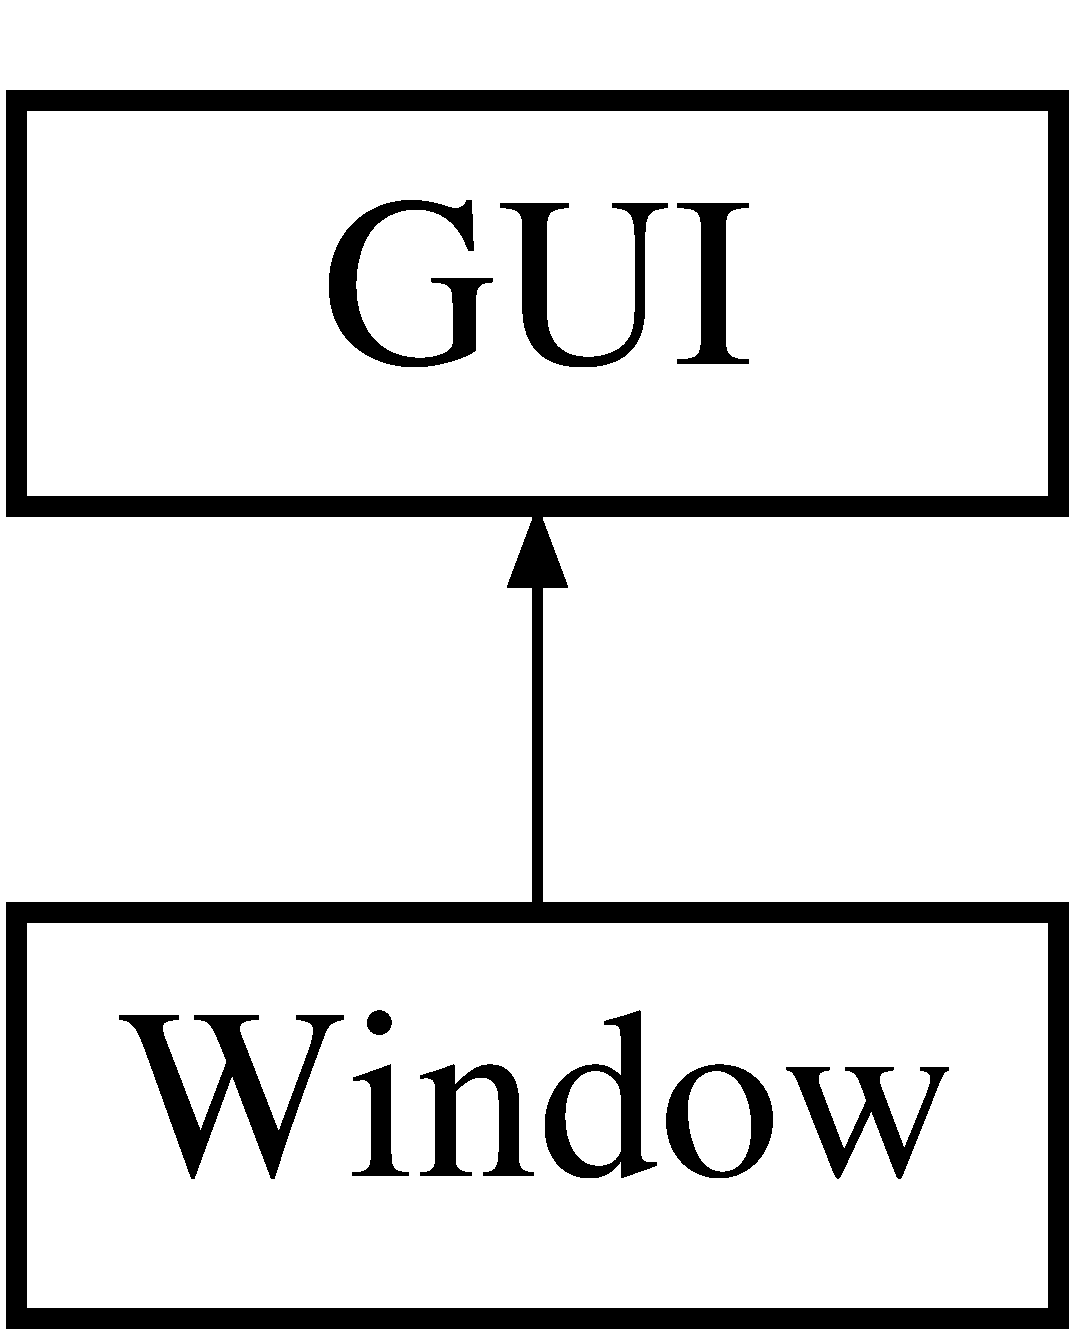
\includegraphics[height=2.000000cm]{class_window}
\end{center}
\end{figure}
\subsection*{Public Types}
\begin{DoxyCompactItemize}
\item 
\mbox{\Hypertarget{class_window_a2ca5739e956b8f5fec8f4e8a9fb1dd92}\label{class_window_a2ca5739e956b8f5fec8f4e8a9fb1dd92}} 
enum {\bfseries Swap\+Interval\+Type} \+: int \{ {\bfseries L\+A\+T\+E\+\_\+\+S\+W\+A\+P\+\_\+\+T\+E\+A\+R\+I\+NG} = -\/1, 
{\bfseries I\+M\+M\+E\+D\+I\+A\+T\+E\+\_\+\+U\+P\+D\+A\+T\+ES} = 0, 
{\bfseries V\+S\+Y\+NC} = 1
 \}
\item 
\mbox{\Hypertarget{class_window_a124fc3e2e9aaf01b362fac1f8896e532}\label{class_window_a124fc3e2e9aaf01b362fac1f8896e532}} 
enum {\bfseries Fullscreen\+Type} \+: Uint32 \{ {\bfseries V\+I\+D\+E\+O\+\_\+\+M\+O\+DE} = S\+D\+L\+\_\+\+W\+I\+N\+D\+O\+W\+\_\+\+F\+U\+L\+L\+S\+C\+R\+E\+EN, 
{\bfseries D\+E\+S\+K\+T\+O\+P\+\_\+\+M\+O\+DE} = S\+D\+L\+\_\+\+W\+I\+N\+D\+O\+W\+\_\+\+F\+U\+L\+L\+S\+C\+R\+E\+E\+N\+\_\+\+D\+E\+S\+K\+T\+OP, 
{\bfseries W\+I\+N\+D\+O\+W\+E\+D\+\_\+\+M\+O\+DE} = 0
 \}
\end{DoxyCompactItemize}
\subsection*{Public Member Functions}
\begin{DoxyCompactItemize}
\item 
\mbox{\Hypertarget{class_window_a0799cc50a89cc6d5e1cd98e71791200d}\label{class_window_a0799cc50a89cc6d5e1cd98e71791200d}} 
{\bfseries Window} (int w=800, int h=600, std\+::string title=\char`\"{}Untitled\char`\"{})
\item 
\mbox{\Hypertarget{class_window_a8ffc0093a40fa9c91f060818444ce4a1}\label{class_window_a8ffc0093a40fa9c91f060818444ce4a1}} 
{\bfseries Window} (const \mbox{\hyperlink{class_window}{Window}} \&copy)
\item 
\mbox{\Hypertarget{class_window_aa4086debceb557ecb6443cce32b41f9b}\label{class_window_aa4086debceb557ecb6443cce32b41f9b}} 
{\bfseries Window} (\mbox{\hyperlink{class_window}{Window}} \&\&move)=delete
\item 
\mbox{\Hypertarget{class_window_a96e2d69af0539f4a45c04cf54803f5ec}\label{class_window_a96e2d69af0539f4a45c04cf54803f5ec}} 
\mbox{\hyperlink{class_window}{Window}} \& {\bfseries operator=} (const \mbox{\hyperlink{class_window}{Window}} \&rhs)=delete
\item 
\mbox{\Hypertarget{class_window_aa63a9a2404cebe562174a851f2dc8a01}\label{class_window_aa63a9a2404cebe562174a851f2dc8a01}} 
virtual void {\bfseries update} () override
\item 
\mbox{\Hypertarget{class_window_ac11084e8bd2b61ba1a45266a9a4a0b57}\label{class_window_ac11084e8bd2b61ba1a45266a9a4a0b57}} 
virtual void {\bfseries destroy} () override
\item 
\mbox{\Hypertarget{class_window_af79c5fde03ed3825e0459a267ea01dee}\label{class_window_af79c5fde03ed3825e0459a267ea01dee}} 
virtual bool {\bfseries focused} () const override
\item 
\mbox{\Hypertarget{class_window_a43a34a3321d0a9bd30dbba747af14c6a}\label{class_window_a43a34a3321d0a9bd30dbba747af14c6a}} 
virtual bool {\bfseries is\+\_\+window} () const override
\item 
\mbox{\Hypertarget{class_window_ab2af2ee909ac87876fd043acfe7611ca}\label{class_window_ab2af2ee909ac87876fd043acfe7611ca}} 
virtual float {\bfseries get\+\_\+window\+\_\+pos\+\_\+x} () const override
\item 
\mbox{\Hypertarget{class_window_a950ef0cfbccf484315041162942c4ecc}\label{class_window_a950ef0cfbccf484315041162942c4ecc}} 
virtual float {\bfseries get\+\_\+window\+\_\+pos\+\_\+y} () const override
\item 
\mbox{\Hypertarget{class_window_ae70c9e2fddb5224f884291b6d8225fe4}\label{class_window_ae70c9e2fddb5224f884291b6d8225fe4}} 
virtual void {\bfseries set\+\_\+hidden} (bool hidden) override
\item 
\mbox{\Hypertarget{class_window_a95d3193d85c5f8ffed21eeef995602f7}\label{class_window_a95d3193d85c5f8ffed21eeef995602f7}} 
bool {\bfseries is\+\_\+close\+\_\+requested} () const
\item 
\mbox{\Hypertarget{class_window_a73b7959b6435d574d5ddbb6115153724}\label{class_window_a73b7959b6435d574d5ddbb6115153724}} 
Swap\+Interval\+Type {\bfseries get\+\_\+swap\+\_\+interval\+\_\+type} () const
\item 
\mbox{\Hypertarget{class_window_a86607cca316a63361a8e0546d7461496}\label{class_window_a86607cca316a63361a8e0546d7461496}} 
void {\bfseries set\+\_\+swap\+\_\+interval\+\_\+type} (Swap\+Interval\+Type type) const
\item 
\mbox{\Hypertarget{class_window_a56c2030999233ae438cb86229bbf1fa8}\label{class_window_a56c2030999233ae438cb86229bbf1fa8}} 
void {\bfseries set\+\_\+title} (const std\+::string \&new\+\_\+title)
\item 
\mbox{\Hypertarget{class_window_a2b9672924d8048d74098deeb4202dc76}\label{class_window_a2b9672924d8048d74098deeb4202dc76}} 
bool {\bfseries is\+\_\+fullscreen} () const
\item 
\mbox{\Hypertarget{class_window_aba76e9ee7a1fc05a26340154244bd967}\label{class_window_aba76e9ee7a1fc05a26340154244bd967}} 
Fullscreen\+Type {\bfseries get\+\_\+fullscreen} () const
\item 
\mbox{\Hypertarget{class_window_ae2ed6e396cf3dd2eb2636951192949cf}\label{class_window_ae2ed6e396cf3dd2eb2636951192949cf}} 
void {\bfseries set\+\_\+fullscreen} (Fullscreen\+Type type) const
\item 
\mbox{\Hypertarget{class_window_a4d69ff4818898cd74241214183f404f9}\label{class_window_a4d69ff4818898cd74241214183f404f9}} 
void {\bfseries set\+\_\+render\+\_\+target} () const
\item 
\mbox{\Hypertarget{class_window_a0df947eae50ea0565b4b5d826b94a394}\label{class_window_a0df947eae50ea0565b4b5d826b94a394}} 
void {\bfseries clear\+\_\+focus} ()
\item 
\mbox{\Hypertarget{class_window_a8ad58be4ce5aec15ad590ce151d4776a}\label{class_window_a8ad58be4ce5aec15ad590ce151d4776a}} 
void {\bfseries clear} (G\+Lbitfield mask=(G\+L\+\_\+\+C\+O\+L\+O\+R\+\_\+\+B\+U\+F\+F\+E\+R\+\_\+\+B\+IT$\vert$G\+L\+\_\+\+D\+E\+P\+T\+H\+\_\+\+B\+U\+F\+F\+E\+R\+\_\+\+B\+IT$\vert$G\+L\+\_\+\+S\+T\+E\+N\+C\+I\+L\+\_\+\+B\+U\+F\+F\+E\+R\+\_\+\+B\+IT), float r=0.\+0f, float g=0.\+0f, float b=0.\+0f, float a=1.\+0f) const
\item 
\mbox{\Hypertarget{class_window_ac5636a14c1078143a869821a07498cd5}\label{class_window_ac5636a14c1078143a869821a07498cd5}} 
void {\bfseries register\+\_\+listener} (\mbox{\hyperlink{class_listener}{Listener}} \&l)
\item 
\mbox{\Hypertarget{class_window_a184dd18eea525b2d4f85a42e33681951}\label{class_window_a184dd18eea525b2d4f85a42e33681951}} 
void {\bfseries deregister\+\_\+listener} (\mbox{\hyperlink{class_listener}{Listener}} \&l)
\item 
\mbox{\Hypertarget{class_window_af2f8beb54b28dc32d93f6b5f403d2152}\label{class_window_af2f8beb54b28dc32d93f6b5f403d2152}} 
\mbox{\hyperlink{class_g_u_i}{G\+UI}} $\ast$ {\bfseries get\+\_\+focused\+\_\+child} () const
\item 
\mbox{\Hypertarget{class_window_abed0ae68fac68c8d2191d4c7d7a82497}\label{class_window_abed0ae68fac68c8d2191d4c7d7a82497}} 
void {\bfseries set\+\_\+focused\+\_\+child} (\mbox{\hyperlink{class_g_u_i}{G\+UI}} $\ast$child)
\end{DoxyCompactItemize}
\subsection*{Additional Inherited Members}


\subsection{Detailed Description}
Topaz Windows used to draw on the screen. Topaz\textquotesingle{}s graphics module will not initialise fully until at least one instance of this class is instantiated. 

The documentation for this class was generated from the following files\+:\begin{DoxyCompactItemize}
\item 
src/graphics/gui.\+hpp\item 
src/graphics/gui.\+cpp\end{DoxyCompactItemize}

%--- End generated contents ---

% Index
\backmatter
\newpage
\phantomsection
\clearemptydoublepage
\addcontentsline{toc}{chapter}{Index}
\printindex

\end{document}
